%  ========================================================================
%  Copyright (c) 1985 The University of Washington
%
%  Licensed under the Apache License, Version 2.0 (the "License");
%  you may not use this file except in compliance with the License.
%  You may obtain a copy of the License at
%
%      http://www.apache.org/licenses/LICENSE-2.0
%
%  Unless required by applicable law or agreed to in writing, software
%  distributed under the License is distributed on an "AS IS" BASIS,
%  WITHOUT WARRANTIES OR CONDITIONS OF ANY KIND, either express or implied.
%  See the License for the specific language governing permissions and
%  limitations under the License.
%  ========================================================================
%

% This file is the doctoral dissertation of Dan Wang
% It is filed by Dan Wang on 11/19/2020 at the University of Washington
% The author can be reached at daw1230@uw.edu

% Template courtesy of Jim Fox at UW
%
 
\documentclass [11pt, proquest] {uwthesis}[2020/02/24]
 
%
% The following line would print the thesis in a postscript font 

% \usepackage{natbib}
% \def\bibpreamble{\protect\addcontentsline{toc}{chapter}{Bibliography}}

\setcounter{tocdepth}{1}  % Print the chapter and sections to the toc
 

% ==========   Local defs and mods

\usepackage{alltt}  % 
\newenvironment{demo}
  {\begin{alltt}\leftskip3em
     \def\\{\ttfamily\char`\\}%
     \def\{{\ttfamily\char`\{}%
     \def\}{\ttfamily\char`\}}}
  {\end{alltt}}

% metafont font.  If logo not available, use the second form
%
% \font\mffont=logosl10 scaled\magstep1
\let\mffont=\sf
% --- end-of-sample-stuff ---
 
\usepackage{tikz}
\usepackage{pgfplots}
\pgfplotsset{compat=1.11}
\usetikzlibrary{matrix,backgrounds,decorations.pathreplacing,positioning}
\tikzstyle{block} = [draw, rectangle, minimum height=2em, minimum width=4em]
\tikzstyle{sum} = [draw, circle]
\tikzstyle{input} = [coordinate] 
\tikzstyle{output} = [coordinate]
\tikzstyle{pinstyle} = [pin edge={to-,thin,black}]

\usepackage{amssymb}
\usepackage{amsmath}
\usepackage{amsthm}
\usepackage{graphicx}
\usepackage{epstopdf}
\usepackage{multirow,booktabs}

\usepackage{supertabular}
\usepackage{makecell}
\usepackage{textcomp}
\usepackage{cite}

\usepackage{txfonts}
\usepackage{subfig}
\usepackage{multirow,booktabs}

\usepackage{babel}
\usepackage{array}
\usepackage{mathrsfs}

\usepackage[active]{srcltx}
\usepackage{verbatim}
\usepackage{units}
\usepackage{cancel}
\usepackage{xargs}
\PassOptionsToPackage{normalem}{ulem}
\usepackage{ulem}
% \usepackage{etex}

\usepackage{pgfpages}
\usepackage{textcomp}

\ifdefined\d

\global\long\def\tf#1{\text{#1}}

\global\long\def\d{\mathrm{d}}

\global\long\def\e{\mathrm{e}}

\global\long\def\i{\mathrm{i}}

\global\long\def\tr{\operatorname{Tr}}

\global\long\def\pr{\operatorname{Pr}}

\global\long\def\mean{\operatorname{E}}

\global\long\def\E{\operatorname{E}}

\global\long\def\et{\operatorname{E}}

\global\long\def\var{\operatorname{Var}}

\global\long\def\cov{\operatorname{Cov}}

\global\long\def\std{\mathrm{std}}

\global\long\def\eig{\operatorname{eig}}

\global\long\def\re{\operatorname{Re}}

\global\long\def\im{\operatorname{Im}}

\global\long\def\iff{\text{if and only if}}

\global\long\def\adj{\mathrm{adj}}

\global\long\def\ol{\text{open-loop}}

\global\long\def\cl{\text{closed-loop}}

% FONTS

\global\long\def\bsf#1{\textsf{\textbf{#1}}}
 

\global\long\def\lbsf#1{\textsf{\large\textbf{#1}}}
 

\global\long\def\Lbsf#1{\textsf{\Large\textbf{#1}}}
 

\global\long\def\hbsf#1{\textsf{\huge\textbf{#1}}}

% XY MATRIX BLOCK DIAGRAM

\global\long\def\bblk#1{*+[F-]{#1}}
 

\global\long\def\bblkshaded#1{*+[F-,]{#1}}
 

\global\long\def\bblkdashed#1{*+[F--]{#1}}
 

\global\long\def\bblkdotted#1{*+[F.]{#1}}
 

\global\long\def\cblk{*[o]{\circ}}
 

\global\long\def\dotblk{*[F]{}}
 

\global\long\def\arline{\ar@{-}}

\global\long\def\arr{\ar[r]}

\global\long\def\arl{\ar[l]}

\global\long\def\aru{\ar[u]}

\global\long\def\ard{\ar[d]}

\global\long\def\ardashr{\ar@{-->}[r]}

\global\long\def\ardashd{\ar@{-->}[d]}

\global\long\def\ardashl{\ar@{-->}[l]}

\global\long\def\ardashu{\ar@{-->}[u]}

\global\long\def\ardotr{\ar@{..>}[r]}

\global\long\def\ardotu{\ar@{..>}[u]}

\global\long\def\ardotd{\ar@{..>}[d]}

\global\long\def\ardotl{\ar@{..>}[l]}

\global\long\def\arU{\ar@{=>}[u]}

\global\long\def\arL{\ar@{=>}[l]}

\global\long\def\arD{\ar@{=>}[d]}

\global\long\def\arR{\ar@{=>}[r]}

% XY MATRIX SCALING

\providecommand{\xyR}[1]{\xydef@\xymatrixrowsep@{#1}}

% scaling column

\providecommand{\xyC}[1]{\xydef@\xymatrixcolsep@{#1}}

%\newcommand{\xlab}[2]{^(#1){#2}}

\ifdefined\thickframe

\newcommandx\thickframe[2][usedefault, addprefix=\global, 1=1mm, 2=3mm]{\fboxrule#1 \fboxsep#2}

\fi

\ifdefined\thickframe

\renewcommandx\thickframe[2][usedefault, addprefix=\global, 1=1mm, 2=3mm]{\fboxrule#1 \fboxsep#2}

\fi

\global\long\def\deriv#1{\dot{#1}}

\global\long\def\dderiv#1{\ddot{#1}}

\ifdefined\cb

\newcommandx\cb[3][usedefault, addprefix=\global, 1=white]{\fcolorbox{#2}{#1}{$#3$}}

\fi

\fi


\usepackage{mathptmx}

\newtheorem{lemma}{Lemma}
\newtheorem{assumption}{Assumption}
\newtheorem{remark}{Remark}
\newtheorem{definition}{Definition}
\newtheorem{fact}{Fact}
\newtheorem{conjecture}{Conjecture}
\newtheorem{example}{Example}
\newtheorem{theorem}{Theorem}

\usepackage{microtype}


% Define the figures location
\graphicspath{{Figures/}}

\begin{document}
 
% ==========   Preliminary pages
%
% ( revised 2012 for electronic submission )
%

\prelimpages
 
%
% ----- copyright and title pages
%
\Title{Control-oriented Modeling and Multirate Feedback Control\\
        in Laser Powder Bed Fusion Additive Manufacturing}
\Author{Dan Wang}
\Year{2020}
\Program{Department of Mechanical Engineering}

\Chair{Xu Chen}{Assistant Professor}{Department of Mechanical Engineering}
\Signature{Santosh Devasia}
\Signature{Ramulu Mamidala}
\Signature{Behçet Açikmeşe}

\copyrightpage

\titlepage  

 
%
% ----- signature and quoteslip are gone
%

%
% ----- abstract
%


\setcounter{page}{-1}
\abstract{%
A high-precision additive manufacturing process, laser powder bed fusion (LPBF) has enabled unmatched agile manufacturing of a wide range of products from engine components to medical implants. While finite element modeling and closed-loop control have been identified key for predicting and engineering part qualities in LPBF, existing results in each realm are developed in opposite computational architectures wildly different in time scale. This proposal builds a first-instance closed-loop simulation framework by integrating high-fidelity finite element modeling with feedback controls originally developed for general mechatronics systems. By utilizing the output signals (e.g., melt pool width) retrieved from the finite element model (FEM) to directly update the control signals (e.g., laser power) sent to the model, the proposed closed-loop framework enables testing the limits of advanced controls in LPBF and surveying the parameter space fully to generate more predictable part qualities. Along the course of formulating the framework, we verify the FEM by comparing its results with experimental and analytical solutions and then use the FEM to understand the melt-pool evolution induced by the thermomechanical interactions. From there, we build a repetitive control (RC) algorithm and a multirate fractional-order RC to greatly attenuate variations in LPBF.
}
 
%
% ----- contents & etc.
%
\tableofcontents
\listoffigures
\listoftables  % I have no tables
 
%
% ----- glossary 
%
\chapter*{Glossary}      % starred form omits the `chapter x'
\addcontentsline{toc}{chapter}{Glossary}
\thispagestyle{plain}
%
\begin{glossary}
\item[argument] replacement text which customizes a \LaTeX\ macro for
each particular usage.
\item[back-up] a copy of a file to be used when catastrophe strikes
the original.  People who make no back-ups deserve
no sympathy.
\item[control sequence] the normal form of a command to \LaTeX.
\item[delimiter] something, often a character, that indicates
the beginning and ending of an argument.
More generally, a delimiter is a field separator.
\item[document class] a file of macros that tailors \LaTeX\ for
a particular document.  The macros described by this thesis
constitute a document class.
\item[document option] a macro or file of macros
that further modifies \LaTeX\ for
a particular document.  The option {\tt[chapternotes]}
constitutes a document option.
 
\end{glossary}
 
%
% ----- acknowledgments
%
\acknowledgments{
This material is based upon work supported in part by the National
Science Foundation under Grant No. 1953155. We would like to thank
all the reviewers and editors for their insightful comments and great
efforts towards improving this manuscript.
}

%
% ----- dedication
%
\dedication{\begin{center}to my family and friends\end{center}}

%
% end of the preliminary pages
 
 
 
%
% ==========      Text pages
%

\textpages

% =========================================== Part 1
\part{Introduction}
 
% ========== Chapter 1
 
\chapter{Introduction} \label{chap:Background-and-Introduction}

Distinct from conventional subtractive machining, additive manufacturing
(AM) builds a part directly from its digital model by joining materials
layer by layer. In particular, applying high-precision lasers as the energy source, laser powder bed fusion (LPBF) AM has enabled
unprecedented fabrication of complex parts from polymeric and metallic
powder materials. LPBF builds a typical part from many thousands of thin layers. Within
each layer (Fig. \ref{fig:Schematic-of-in-layer}), the laser beam is reflected by mirrors driven by periodic or near-periodic reference signals in a beam deflection mechanism (e.g., a dual-axis
galvo scanner) to follow trajectories predefined by the part geometry
in a ``slicing'' process (see, e.g., Fig. \ref{fig:Schematic-of-laser-scanning}). After the printing of one layer, a recoater
will spread a new thin layer of powder over the just-fused layer,
and then another cycle will begin.

Broader adoption of the technology remains
challenged by insufficient reliability and in-process variations.
These variations are induced by, for example, uncertain laser-material
interactions, environmental vibrations, powder recycling, imperfect
interactions of mechanical components, and complex thermal histories
of materials\cite{wang2018multirate,kruth2007feedback,seyda2012investigation}. Current researches employ finite
element modeling and feedback controls to understand the energy-deposition
mechanisms and to regulate the in-process variations in LPBF. For instance,
\cite{masoomi2017laser,hussein2013finite,foroozmehr2016finite,khairallah2016laser}
adopt finite element modeling to investigate how various scan patterns,
scan speeds, number of lasers, overhanging structures, and underlying
physics affect the thermal fields of the powder bed, the geometries
of the melt pool, and the mechanical properties of the printed parts.
Specially, \cite{debroy2017building} brings up the idea of building
digital twins of AM machines by integrating various high-fidelity
multiphysics models. Existing feedback control strategies usually
implement low-order system models obtained from system identification
techniques, such as \cite{kruth2007feedback,craeghs2010feedback,zheng2020distributed}
in LPBF and \cite{song2011feedback,cao2015control,sammons2014repetitive}
in laser metal deposition (LMD), an AM technology analogous to LPBF.
A nonlinear memoryless submodel \cite{fathi2008geometry,cao2015control}
and a spatial-domain Hammerstein model \cite{sammons2014repetitive}
are further built in LMD to cover more complicated process dynamics.
From there, PID control, sliding mode control, predictive control,
and iterative learning control have proved their efficiencies in improving
the dimensional accuracy of the printed parts in LPBF \cite{kruth2007feedback,craeghs2010feedback,vlasea2015development,fleming2020tracking}
and in LMD \cite{hofman2012camera,salehi2006melt,fathi2007clad,fathi2008geometry,song2011feedback,tang2011layer}.
\begin{figure}[!ht]
\begin{centering}
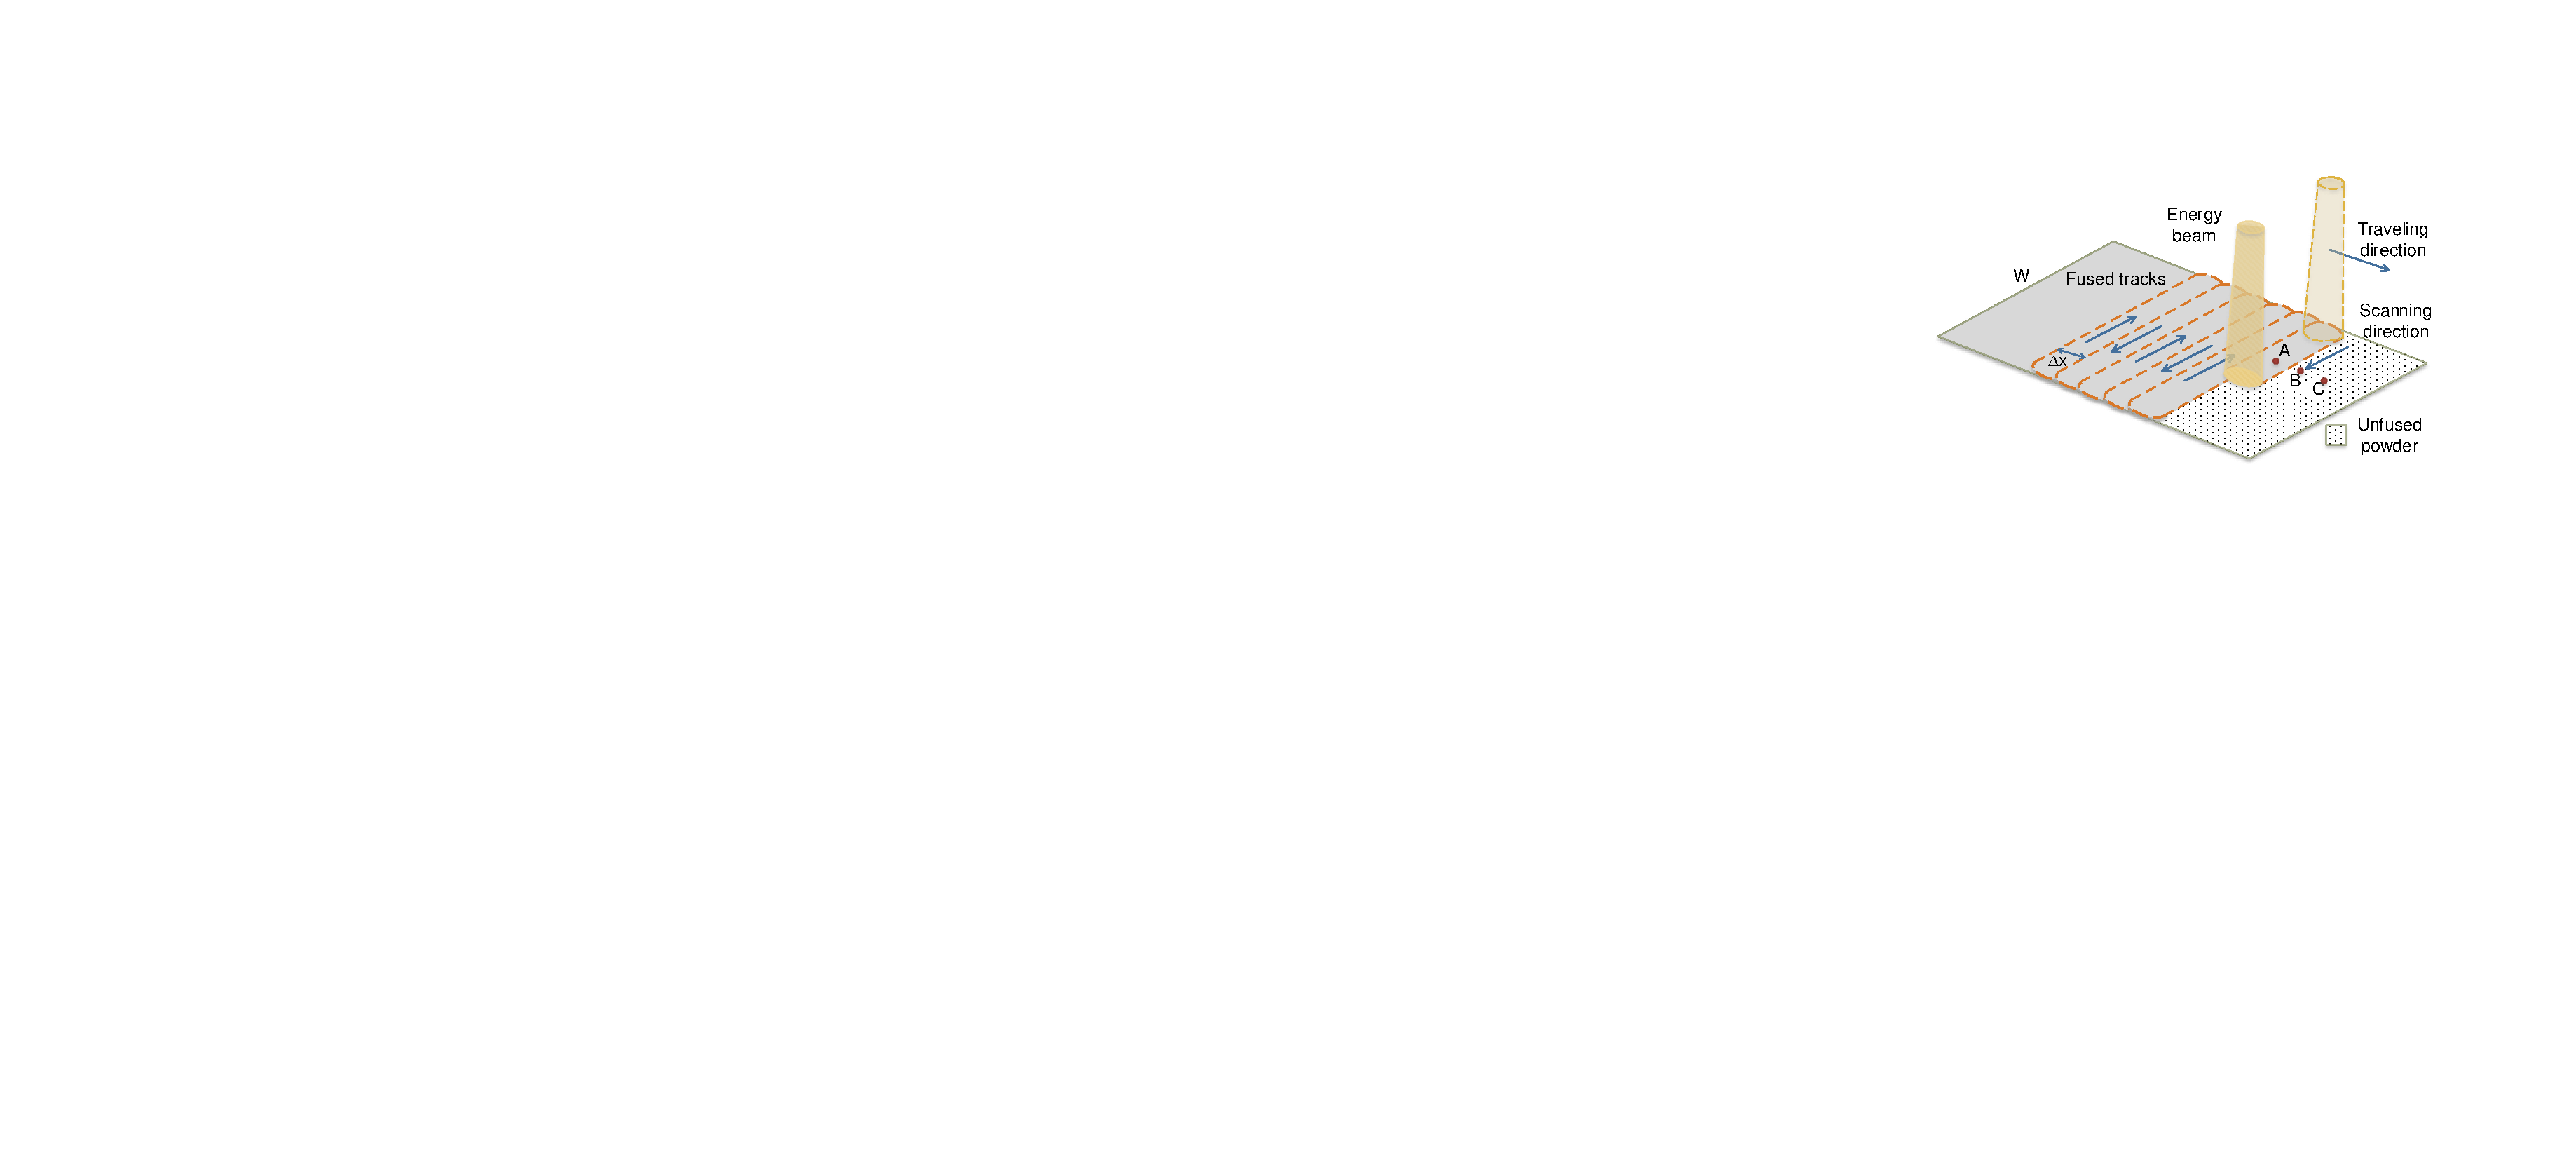
\includegraphics[clip,width=9cm]{Closed-loop-simulation/SLS schematic diagram-2}
\par\end{centering}
\centering{}\caption{\label{fig:Schematic-of-in-layer}Schematic of in-layer LPBF process.}
\end{figure}
\begin{figure}[!ht]
\begin{centering}
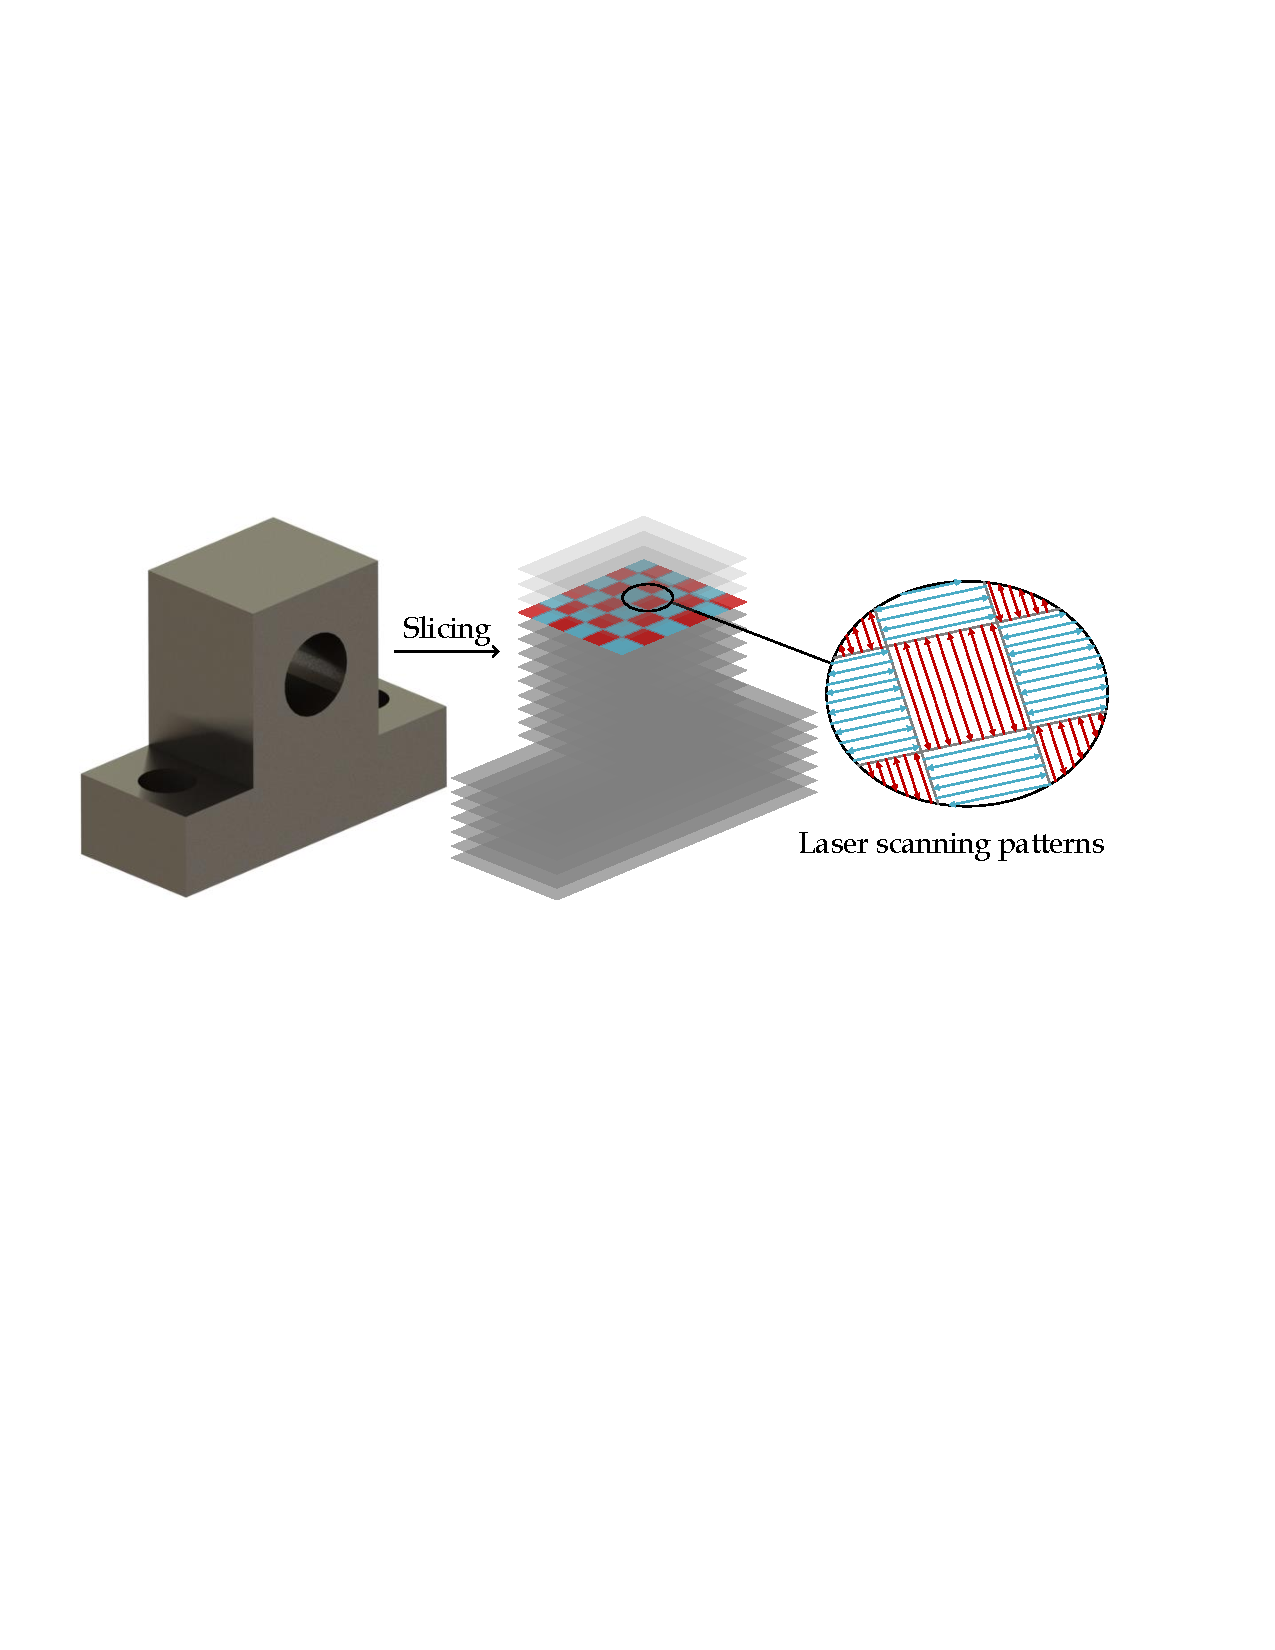
\includegraphics[width=13cm]{Fractional-order-RC/laser scanning patterns_dw}
\par\end{centering}
\caption{\label{fig:Schematic-of-laser-scanning}Schematic of laser scanning patterns
in LPBF. The example shows the most common ``island'' pattern in
LPBF of metallic objects.}
\end{figure}

Although finite element model (FEM) and feedback control have been
identified key for predicting and engineering part qualities in LPBF,
existing results in each realm are developed in separate computational
architectures due to their different time scales. Feedback controls
are implemented in real time, while FEM takes hours or even days to
simulate the printing of a few layers that finishes in seconds in
reality. If we can integrate FEM with feedback controls directly in
a closed loop, however, we can 1) combine aforementioned knowledge
from each realm, 2) test the limit of advanced control in LPBF, 3)
survey the parameter space fully to generate more predictable part
qualities, and 4) quickly design controllers and update parameters
for novel materials and printer settings. These benefits are more
prominent when the experiments are costly and time-consuming.

In pursuit of the above benefits, this dissertation builds, in the first
instance to our best knowledge, a closed-loop high-fidelity simulation
framework that leverages modern architectures of finite-element-modeling
tools and the power of data processing and advanced controls. In particular,
we build a bidirectional architecture so that the output signals (e.g.,
melt pool width or peak temperature) retrieved from the FEM can be
utilized to directly update the FEM process parameters (e.g., laser
power or scan speed) in external control toolboxes (e.g., MATLAB).
In this way, we design an interface that enables simulating closed-loop
controllers for LPBF thermal processes. Along the course of formulating
the framework, XXXXX

The major contributions of this chapter are:

\begin{itemize}
\item developing a closed-loop simulation architecture for implementing
and testing out feedback control strategies in FEM;
\item building an RC algorithm and an FEM of the LPBF thermal process, as
applications of the proposed architecture;
\item verifying the effectiveness of RC in regulating the periodic thermal
interactions in LPBF.
\end{itemize}
The remainder of this chapter is structured as follows. Section \ref{chap:Closed-loop-Simulation}
frames the main closed-loop high-fidelity simulation with the bidirectional
architecture between FEM and controller. As application examples,
Chapter \ref{chap:FEM} develops an FEM of the
thermal fields in LPBF, and Section xxx
builds an RC design to regulate the periodic thermal cycles. Under
the architecture of the closed-loop simulation, Section \ref{chap:RC-Closed-loop-Simulation}
evaluates the performance of RC. Section concludes
the chapter.

% Fractional-order Repetitive control
This chapter discusses fractional-order repetitive control (RC) to advance
the quality of periodic energy deposition in laser-based additive
manufacturing (AM). It addresses an intrinsic RC limitation when the
exogenous signal frequency cannot divide the sampling frequency of
the sensor, e.g., in imaging-based control of fast laser-material
interaction in AM. Three RC designs are proposed to address such fractional-order
repetitive processes. In particular, a new multirate RC provides superior
performance gains by generating high-gain control exactly at the fundamental
and harmonic frequencies of exogenous signals. Experimentation on
a galvo laser scanner in AM validates effectiveness of the designs.

% Closed-loop simulation
A high-precision additive manufacturing process, powder bed
fusion (PBF) has enabled unmatched agile manufacturing of a wide range
of products from engine components to medical implants. While finite
element modeling and closed-loop control have been identified key
for predicting and engineering part qualities in LPBF, existing results
in each realm are developed in opposite computational architectures
wildly different in time scale. This chapter builds a first-instance
closed-loop simulation framework by integrating high-fidelity finite
element modeling with feedback controls originally developed for general
mechatronics systems. By utilizing the output signals (e.g., melt
pool width) retrieved from the finite element model (FEM) to update
directly the control signals (e.g., laser power) sent to the model,
the proposed closed-loop framework enables testing the limits of advanced
controls in LPBF and surveying the parameter space fully to generate
more predictable part qualities. Along the course of formulating the
framework, we verify the FEM by comparing its results with experimental
and analytical solutions and then use the FEM to understand the melt-pool
evolution induced by the in- and cross-layer thermomechanical interactions.
From there, we build a repetitive control algorithm to attenuate variations
of the melt pool width.

% Model inversion
Stably inverting a dynamic system model is fundamental to subsequent
servo designs. Current inversion techniques have provided effective
model matching for feedforward controls. However, when the inverse
models are to be implemented in feedback systems, additional considerations
are demanded for assuring causality, robustness, and stability under
closed-loop constraints. To bridge the gap between accurate model
approximations and robust feedback performances, this chapter provides
a new treatment of unstable zeros in inverse design. We provide first
an intuitive pole-zero-map-based inverse tuning to verify the basic
principle of the unstable-zero treatment. From there, for general
nonminimum-phase and unstable systems, we propose an optimal inversion
algorithm that can attain model accuracy at the frequency regions
of interest while constraining noise amplification elsewhere to guarantee
system robustness. Along the way, we also provide a modern review
of model inversion techniques. The proposed algorithm is validated
on motion control systems and complex high-order systems.

% Spectral analysis
A fundamental challenge in sampled-data control arises when a continuous-time plant is subject to disturbances that possess significant frequency components beyond the Nyquist frequency of the feedback sensor. Such intrinsic difficulties create formidable barriers for fast high-performance controls in modern and emerging technologies such as additive manufacturing and vision servo, where the update speed of sensors is low compared to the dynamics of the plant. This chapter analyzes spectral properties of closed-loop signals under such scenarios, with a focus on mechatronic systems. We propose a spectral analysis method that provides new understanding of the time- and frequency-domain sampled-data performance. Along the course of uncovering spectral details in such beyond-Nyquist controls, we also report a fundamental understanding on the infeasibility of single-rate high-gain feedback to reject disturbances not only beyond but also below the Nyquist frequency. New metrics and tools are then proposed to systematically quantify the limit of performance. Validation and practical implications of the limitations are provided with experimental case studies performed on a precision mirror galvanometer platform for laser scanning.

% Loop shaping
Many servo systems require micro/nano level positioning accuracy. This requirement sets a number of challenges from the viewpoint of sensing, actuation, and control algorithms. This chapter considers control algorithms for precision positioning. We examine how prior knowledge about the parameterization of control structure and the disturbance spectrum should be utilized in the design of control algorithms. An outer-loop inverse-based Youla-Kucera parameterization is built in the chapter. The presented algorithms are evaluated on a tutorial example of a galvo scanner system.

% Hammerstein
Despite the advantages and emerging applications, broader adoption
of powder bed fusion (PBF) additive manufacturing is challenged by
insufficient reliability and in-process variations. Finite element
modeling and control-oriented modeling have been identified fundamental
for predicting and engineering part qualities in LPBF. This chapter first
builds a finite element model (FEM) of the thermal fields to look
into the convoluted thermal interactions during the LPBF process. Using
the FEM data, we identify a novel surrogate system model from the
laser power to the melt pool width. Linking a linearized model with
a memoryless nonlinear submodel, we develop a physics-based Hammerstein
model that captures the complex spatiotemporal thermomechanical dynamics.
We verify the accuracy of the Hammerstein model using the FEM and
prove that the linearized model is only a representation of the Hammerstein
model around the equilibrium point. Along the way, we conduct the
stability and robustness analyses and formalize the Hammerstein model
to facilitate the subsequent control designs.

% =========================================== Part 2

\part{Closed-loop High-fidelity Simulation} \label{part:Closed-loop-Simulation}

% ========== Chapter 2

\chapter{Architecture of Closed-loop High-fidelity Simulation} \label{chap:Closed-loop-Simulation}

We propose in this chapter the main closed-loop simulation that integrates
FEM with feedback controls directly in a closed loop. The key idea
is to use the output signals (e.g., melt pool width) retrieved from
the FEM to update through the controller the control signals (e.g.,
laser power) sent back to the FEM. The core of the FEM is the numerical
simulation of a partial differential equation (PDE) of the general
form:
\[
f(x_{1},\ldots,x_{n};u,\frac{\partial u}{\partial x_{1}},\ldots,\frac{\partial u}{\partial x_{n}};\frac{\partial^{2}u}{\partial x_{1}\partial x_{1}},\ldots,\frac{\partial^{2}u}{\partial x_{1}\partial x_{n}};\ldots)=0,
\]
where $u$ is the output signal predicted by the FEM and $x_{1},\ldots,x_{n}$
are the independent variables. Examples of PDEs in LPBF include the
governing equations for heat transfer, thermal stress, and fluid flow;
the output signals are hence the temperature, stress, and melt pool
velocity, respectively \cite{luo2018survey,mukherjee2018heat}. On
the other hand, in feedback control, an output signal is compared
with a reference signal to generate an error signal, which is then
filtered by a controller to produce a control signal. By reacting
to the in-process change of the output signal, feedback control compensates
for model inaccuracies and unmeasured disturbances.

Leveraging the power of FEM and feedback controls, we develop the
closed-loop simulation algorithm and outline its workflow as follows:
\begin{enumerate}
\item Designing and initializing the FEM in an FEM software (e.g., COMSOL) and the controller in a control-oriented scripting programming environment (abbreviated as programming 
environment, e.g., MATLAB). For the focused closed-loop FEM in this chapter, we set the computation time of the FEM as $t_{s}$, where $t_{s}$ is the sampling time of the discrete-time feedback loop;
\item Building an interface to connect the FEM software with the programming
environment. This interface enables simulating closed-loop controllers
for FEM and taking advantage of the programming environment in preprocessing,
model manipulation, statistical analysis, and post-processing; 
\item \label{enu:Through-the-interface,}Through the interface, the programming
environment retrieves the output signal from the FEM software. Thereafter,
the controller processes the output signal to get the new control
signal, which is then sent back to the FEM. With the updated control
signal, a new FEM computation begins;
\item Repeating step \ref{enu:Through-the-interface,} until the whole simulation
ends.
\end{enumerate}
With the bidirectional architecture between the FEM and controller,
the closed-loop simulation enables updating directly the control signals
of the FEM, retrieving signals hard to reach by experiments, and surveying
the parameter space fully before real LPBF experiments. Moreover, the
proposed architecture is agnostic to the types of programming environment
and FEM software, facilitating incorporating various control methods
into different multiphysics simulations (e.g., heat transfer and fluid
flow studies). As application examples, we choose COMSOL Multiphysics,
MATLAB, and \emph{LiveLink for MATLAB} to build the FEM, controller,
and interface, respectively. We provide in this chapter the skeletons
of an FEM of the thermal fields and a feedback control design. We
will build the detailed FEM and controller in Parts \ref{part:Control-oriented Modeling}
and \ref{part:Multirate-Feedback-Control}, respectively.

1) The governing equation for the conduction heat flow in LPBF is
\begin{equation}
\rho c_{p}\frac{dT(x,\,y,\,z,\,t)}{dt}=\nabla\cdot(k\nabla T(x,\,y,\,z,\,t))+q_{s},\label{eq:heat_conduction}
\end{equation}

\noindent where $k$ is the thermal conductivity, $c_{p}$ the specific
heat capacity, $\rho$ the effective density, $t$ the time, $T$
the temperature, and $q_{s}$ the rate of local internal energy generated
per unit volume \cite{kannatey2009principles}. When no confusion
would arise in the context, we abbreviate $T(x,\,y,\,z,\,t)$ to $T$
in the rest of this dissertation.

The initial condition is defined by setting $T(x,\,y,\,z,\,0)$ as
the ambient temperature $T_{0}$. When the substrate (Fig. \ref{fig:Mesh-and-scan})
is designed to be large enough compared to the heat-affected zone,
one boundary condition is established by assuming the bottom ($z=h$)
of the substrate has no heat loss \cite{masoomi2017laser,hussein2013finite,foroozmehr2016finite}:
$\left.-k\frac{\partial T}{\partial z}\right\vert _{z=h}=0$. A quantitative
way to test and validate the size of the substrate is that from the
FEM results, the bottom of the substrate should maintain the temperature
of $T_{0}$. The other boundary condition is established by considering
the top surface ($z=0$) of the powder bed with input heat flux, convection
heat loss, and radiation heat loss:

\begin{equation}
\left.-k\frac{\partial T}{\partial z}\right\vert _{z=0}=-Q+h_{c}(T-T_{0})+\varepsilon\sigma_{B}(T^{4}-T_{0}^{4}),\label{eq:first_one_boundary}
\end{equation}

\noindent where $Q$ is the input heat flux, $h_{c}$ the convection
heat transfer coefficient, $\varepsilon$ the emissivity, and $\sigma_{B}$
the Stefan-Boltzmann constant. Here, we assume $Q$ has a Gaussian
laser beam profile: $Q\thickapprox\frac{2q}{\pi R^{2}}\text{e}^{-\frac{2r^{2}}{R^{2}}}$,
where $q$ is the laser power, $R$ the effective laser beam radius,
and $r$ the radial distance from a certain point to the center of
the laser spot. From the temperature distribution predicted by the
FEM, melt pool width can be further calculated, as will be elaborated
in Section \ref{chap:FEM}. From here on, we select melt pool width
$w$ as the output signal and laser power $q$ as the control signal
for the subsequent feedback control design. 

\begin{figure}[!ht]
\begin{centering}
% \resizebox{10cm}{!}{%
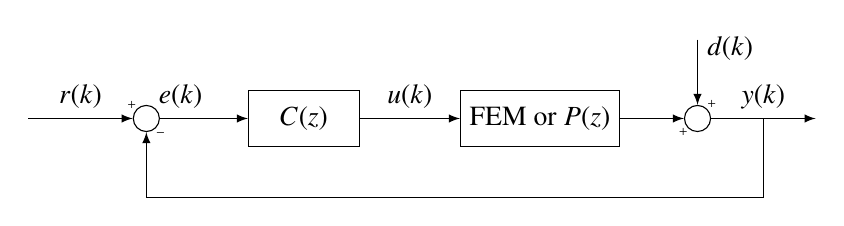
\begin{tikzpicture}[auto, node distance=2cm, >=latex] 

\node [input, name=input] {}; 
\node [sum, right of=input, node distance=1.5cm] (sum) {};
\node [coordinate, right of=sum, xshift = 0.4cm, node distance=0.3cm] (sumC) {};

\node [block, right of=sum] (controller) {$C(z)$}; 

\node [block, right of=controller, node distance=3cm] (plant) {FEM or $P(z)$};
\node [sum, right of=plant](sum3) {};
\node [output, right of=sum3, node distance=1.5cm] (output) {};

\node [coordinate, below of=controller, xshift = 0.2cm, node distance=1cm] (measurements) {};

\node [input, above of=sum3, node distance=1cm](disturbance) {};
\draw [->] (disturbance) -- node [yshift = 0.3cm]{$d(k)$} node[pos=0.99] {\tiny $+$} (sum3);

\draw [->] (input) -- node {$r(k)$} node[pos=0.99] {\tiny $+$} (sum); 
\draw (sum) -- node {$e(k)$} (sumC); 
\draw [->] (sumC) -- (controller);
\draw [->] (controller) -- node{$u(k)$} (plant);

\draw [->] (plant) -- node[below, pos=0.99] {\tiny $+$} (sum3);

\draw [->] (sum3) -- node (y) {$y(k)$}(output); 
\draw [-] (y) |- (measurements); 
\draw [->] (measurements) -| node[right, pos=0.99] {\tiny $-$}(sum);

\end{tikzpicture}
% }
\par\end{centering}
\caption{\label{fig:Block-diagram-of-fb}Block diagram of general feedback control.}
\end{figure}
2) A generic feedback system consists of a plant $P(z)$ and a controller
$C(z)$ (Fig. \ref{fig:Block-diagram-of-fb}). In this study, $P(z)$
is the plant model identified from the FEM simulation. The signal
$r(k)$ represents the system reference, which here is a desired melt
pool width; $u(k)$ represents the control signal, which here is the
laser power; $y(k)$ represents the system output, which here is the
melt pool width as calculated from FEM-predicted temperature fields;
$d(k)$ represents the input disturbance, which here is the in-process
melt-pool-width variations.

\begin{figure}[!ht]
\begin{centering}
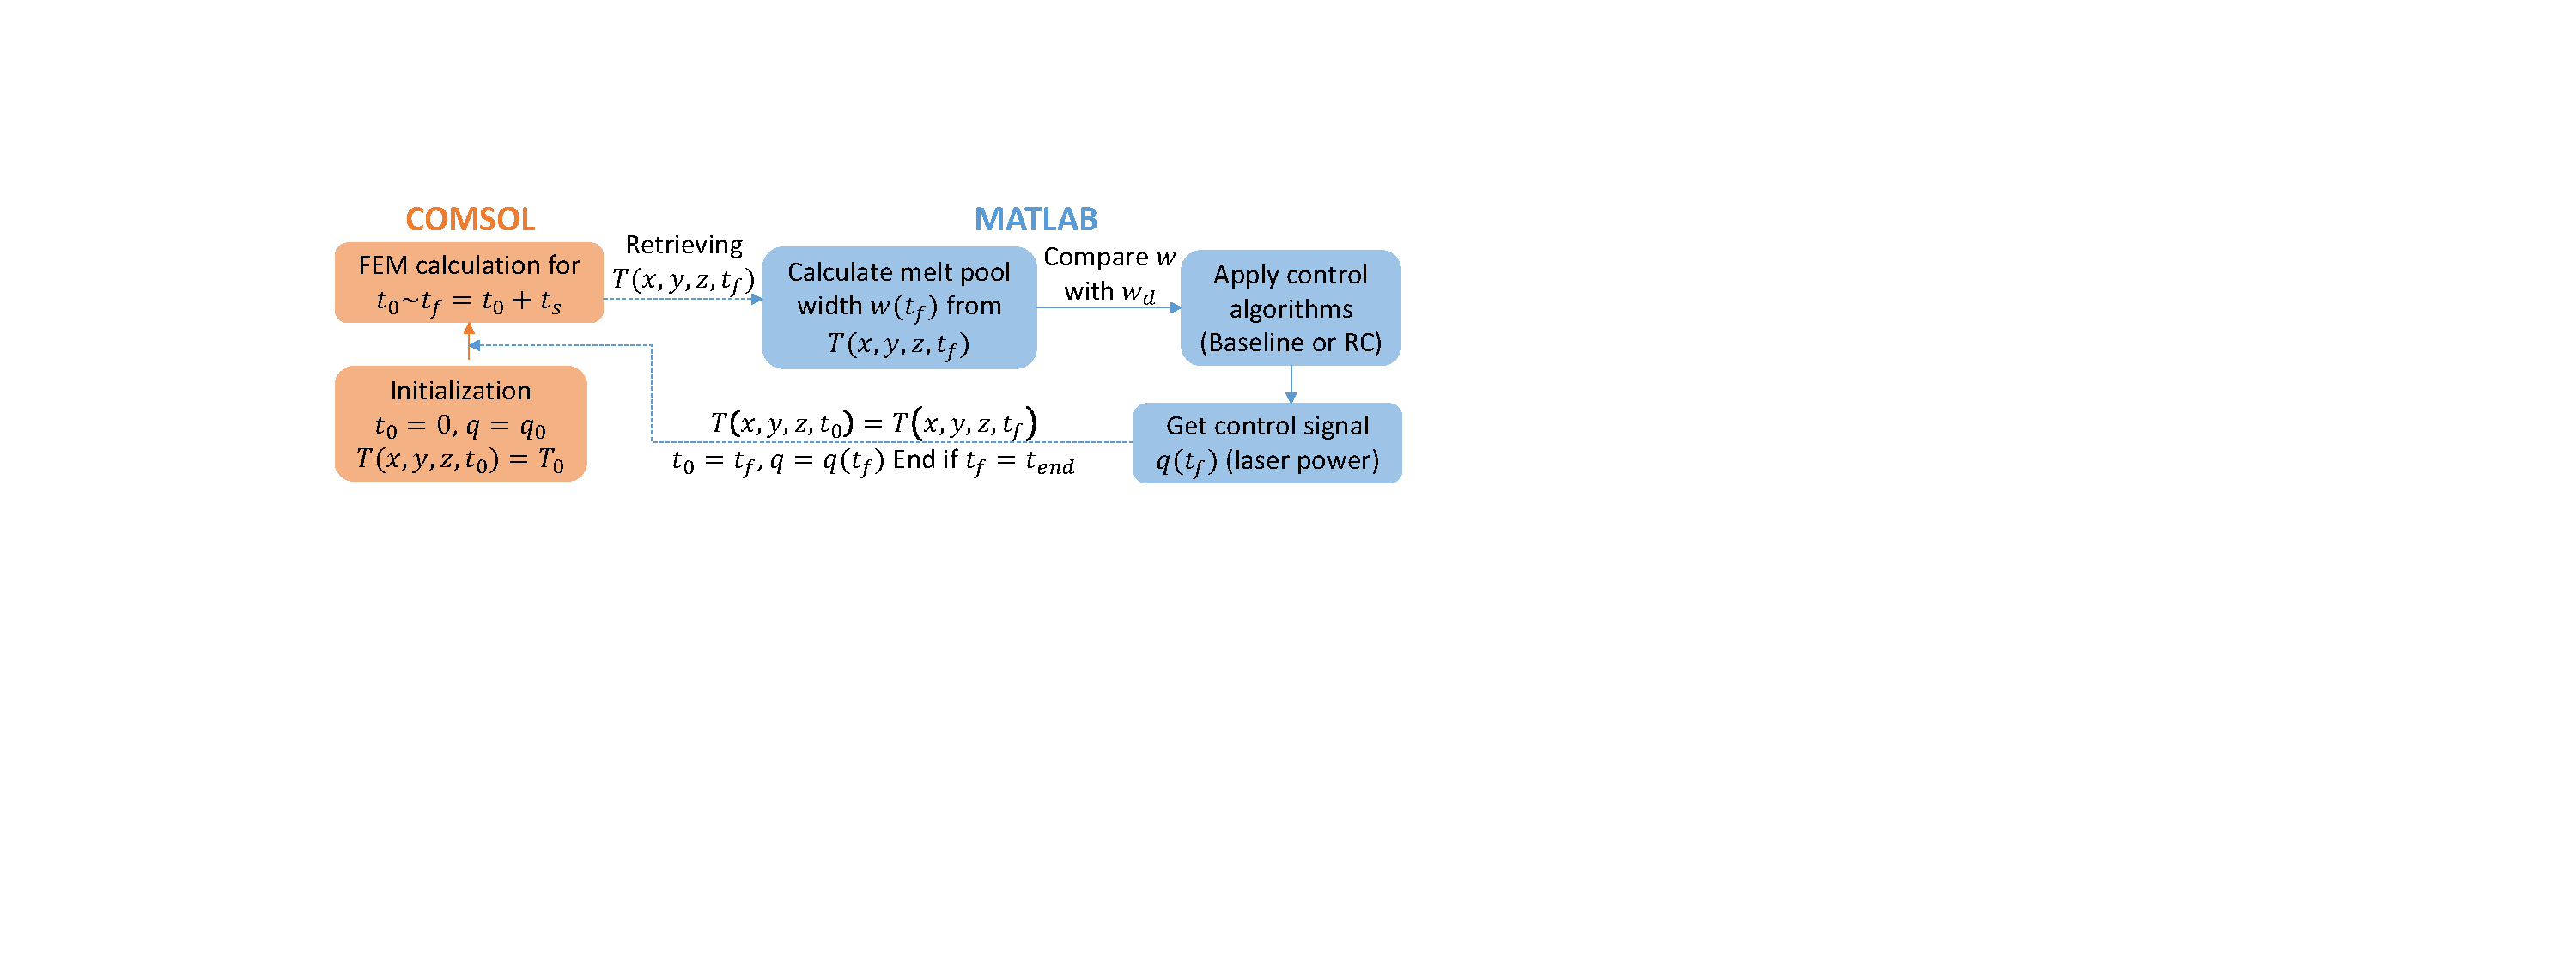
\includegraphics[clip,width=13cm]{Closed-loop-simulation/closedloop_comsol_matlab_2}
\par\end{centering}
\centering{}\caption{\label{fig:Schematic-of-proposed}Schematic of proposed closed-loop
simulation.}
\end{figure}
Fig. \ref{fig:Schematic-of-proposed} demonstrates the operating procedures
of the proposed closed-loop simulation architecture, taking as examples
the FEM of the LPBF thermal process and general feedback control. We
design and initialize the FEM in COMSOL while programming in MATLAB
the main file of the architecture that includes the interface establishment,
the controller design, and the recursive calls for COMSOL. First,
we initialize the FEM by setting the start time $t_{0}$ as 0, the
laser power $q$ as an initial value $q_{0}$, and the temperature
distribution $T(x,\,y,\,z,\,t_{0})$ as the ambient temperature $T_{0}$.
The computation time of the FEM is set as one time step from $t_{0}$
to $t_{f}=t_{0}+t_{s}$. After the initialization, MATLAB will call
COMSOL to start the FEM computation. After retrieving the FEM-predicted
temperature distribution $T(x,\,y,\,z,\,t_{f})$, the main file in
MATLAB calculates the melt pool width $w(t_{f})$ from $T(x,\,y,\,z,\,t_{f})$
and, based on the control algorithms, processes $w(t_{f})$ and its
historical values to obtain the control signal $q(t_{f})$. After
that, the FEM is updated by assigning the iterative variables $t_{0}$
as $t_{f}$, $T(x,\,y,\,z,\,t_{0})$ as $T(x,\,y,\,z,\,t_{f})$, and
the laser power as $q(t_{f})$. After passing all closed-loop computed
information, MATLAB will call COMSOL to start the FEM computation
with the updated variables, and a new cycle will begin. The closed-loop
simulation will stop when $t_{f}$ reaches to the whole simulation
time $t_{end}$ ($\gg t_{f}$ in general).

\begin{figure}[!ht]
\begin{centering}
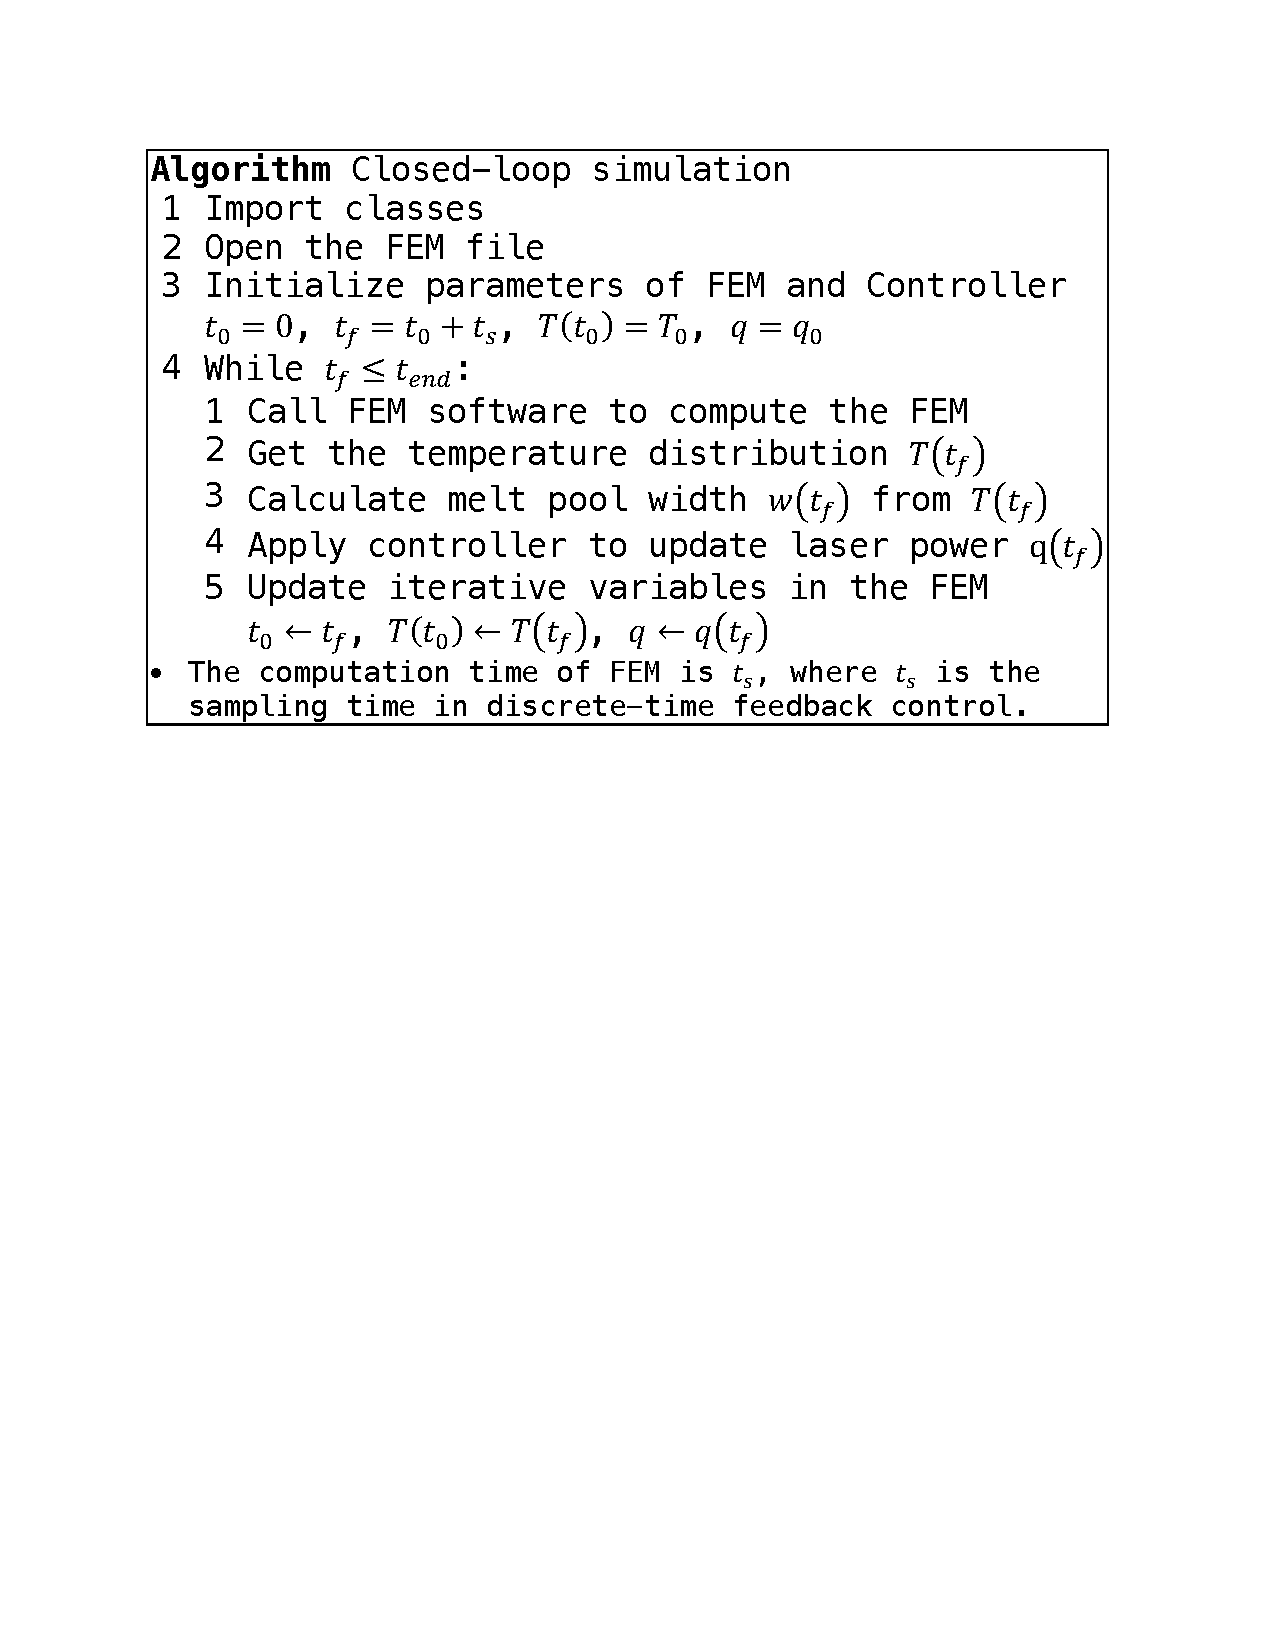
\includegraphics[clip,width=10cm]{Closed-loop-simulation/pseudocode_math}
\par\end{centering}
\centering{}\caption{\label{fig:Pseudocode-for-the}Pseudocode of closed-loop simulation
algorithm.}
\end{figure}
We provide in Fig. \ref{fig:Pseudocode-for-the} the pseudocode of
the main file in the closed-loop simulation algorithm. After importing
the necessary classes for building the FEM, controller, and interface,
the algorithm opens the FEM file and initializes the parameters of
the FEM and controller. Inside the \emph{while} loop, the main file
calls the FEM software to compute the FEM simulation and then retrieves
the predicted temperature distribution $T(x,\,y,\,z,\,t_{f})$. Based
on $T(x,\,y,\,z,\,t_{f})$, the algorithm calculates the melt pool
width $w(t_{f})$ and thereafter processes $w(t_{f})$ and its historical
values through the controller to get the new laser power. At last,
the algorithm updates the iterative variables of the start time, the
initial temperature, and the laser power to get prepared for a new
iteration. Appendix \ref{chapA:MATLAB-commands-closed-loop-simulation} provides the main MATLAB commands used in
the closed-loop simulation.

The proposed closed-loop simulation establishes not only a bidirectional
communication between FEM software and programming environment, but
also an interface specifically for the purpose of simulating feedback
controllers in FEM. The built architecture will benefit and guide
experiments by validating beforehand the effectiveness of the servo
designs. Next we will present the detailed FEM and controller designs
in Parts \ref{part:Control-oriented Modeling} and \ref{part:Multirate-Feedback-Control},
respectively.

% =========================================== Part 3

\part{Control-oriented Modeling} \label{part:Control-oriented Modeling}

% ========== Chapter 3

\chapter{Finite Element Modeling} \label{chap:FEM}

In this chapter, we use the COMSOL Multiphysics 5.3a software to build
and refine the FEM of the temperature response in LPBF, which serves
as an essential component of the proposed closed-loop simulation.
We verify the FEM configuration by comparing the numerical results
with the experimental and analytical solutions and then use the verified FEM to investigate
the periodic in- and cross-layer thermal interactions. The FEM developed
in this chapter considers conduction, latent heat of fusion, surface
convection, and surface radiation. The principal objective of this dissertation is not to create a new high-fidelity FEM at microscopic fluid
flow level but to develop and test the closed-loop simulation architecture.
Therefore, we omit the effects of evaporation, fluid flow, and Marangoni
force for easier testing in the general control community. The FEM
built in this chapter is intended as one application example of the
proposed architecture between FEM and controller. However, the physics
of complex melt flow (e.g., Marangoni and surface tension effects)
can be readily added to increase the model accuracy and provide more
microscopic details of the melt pool that are beyond the focus of
this dissertation.

\section{Finite Element Model} \label{sec:FEM}

\begin{figure*}[!ht]
\begin{centering}
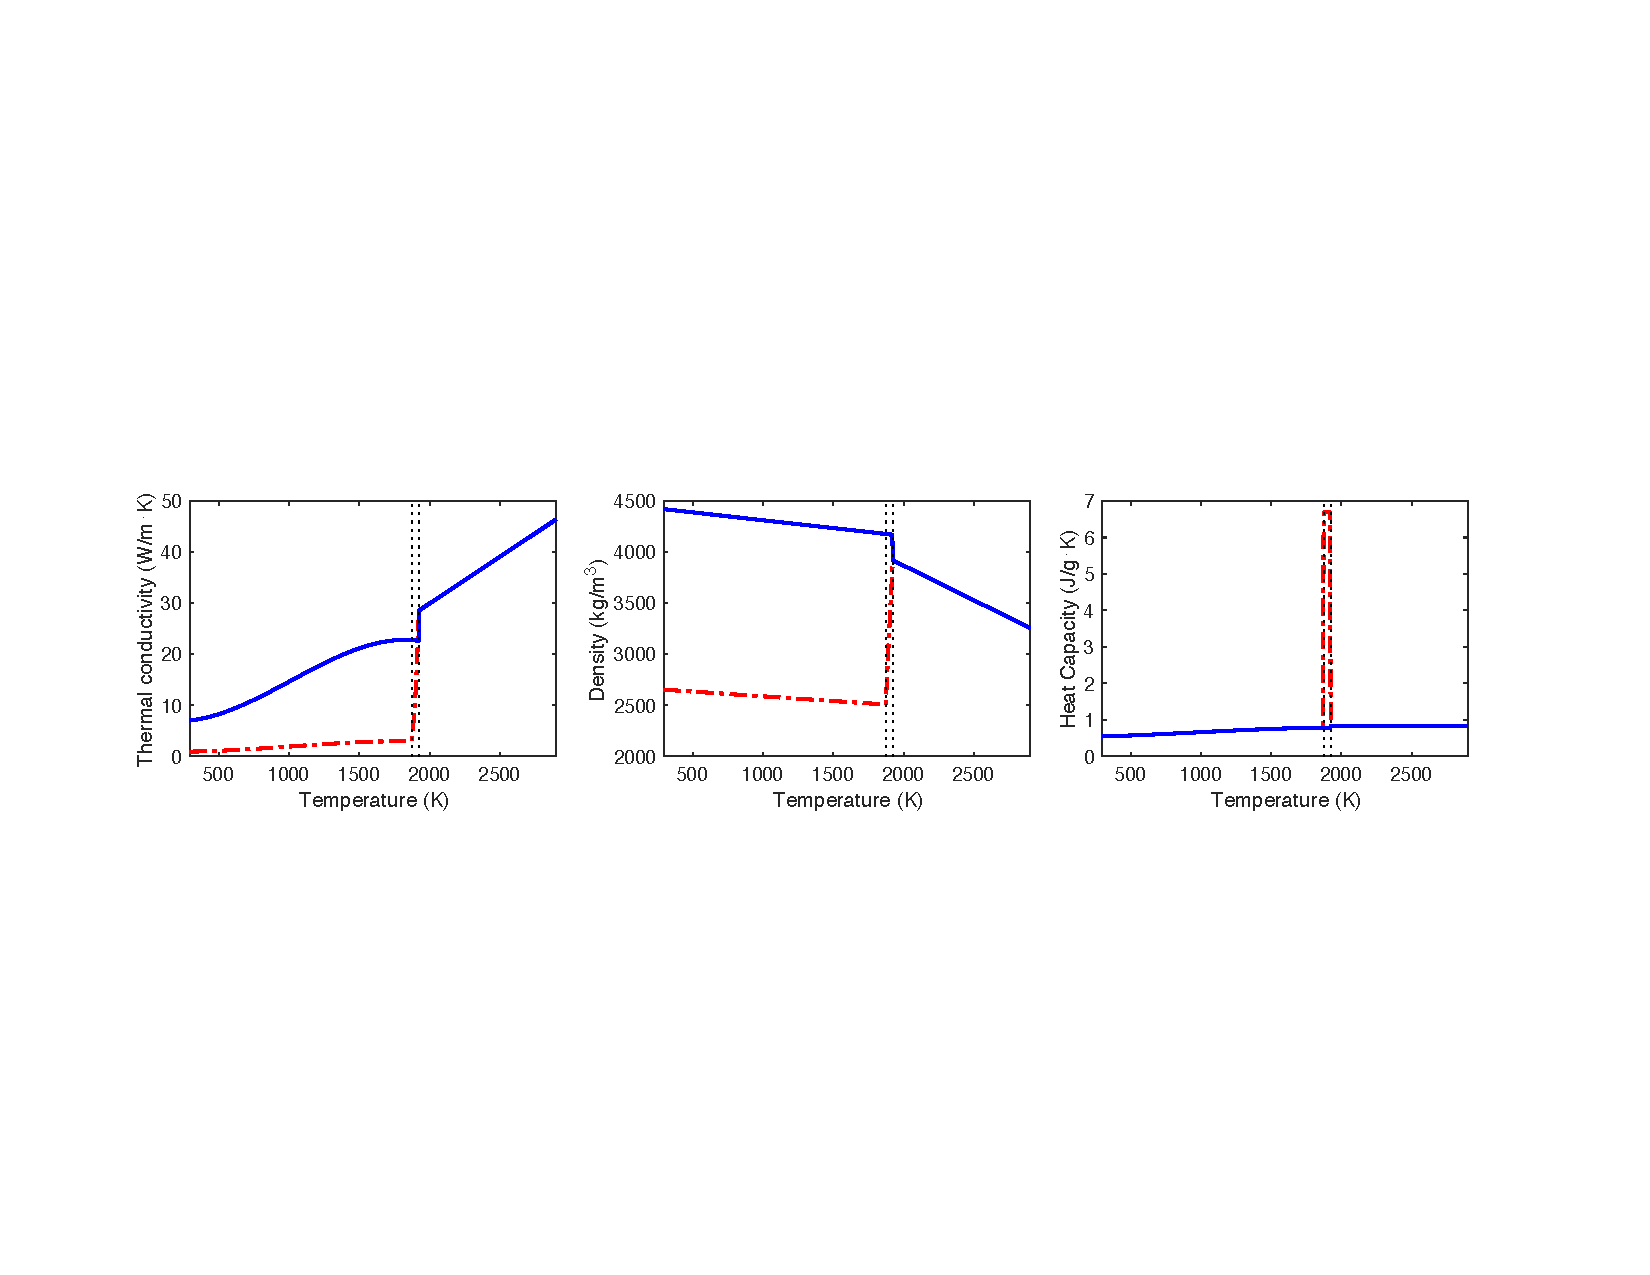
\includegraphics[clip,width=16cm]{Closed-loop-simulation/temp_dependent_thermal_properties}
\par\end{centering}
\centering{}\caption{\label{fig:Temperature-dependent-physical-p}Temperature-dependent
thermal properties of Ti6Al4V.
Solid line: solid and liquid materials. Dash-dotted line: powder material.
The two vertical dotted lines respectively indicate $T_{sol}$ and
$T_{m}$.}
\end{figure*}
We have elaborated the governing equation, initial condition, and
boundary conditions in Chapter \ref{chap:Closed-loop-Simulation}.
For the temperature-dependent thermal properties in (\ref{eq:heat_conduction}),
we adopt $k$, $c_{p}$, and $\rho$ in \cite{masoomi2017laser,arce2012thermal}
for the solid and liquid materials, as shown in Fig. \ref{fig:Temperature-dependent-physical-p}.
We generate the thermal properties of the powder material from those
of the solid material by considering the powder-bed porosity $\phi$
\cite{karayagiz2019numerical,yin2012simulation}:

\begin{align*}
k_{powder} & =k_{solid}(1-\phi)^{4}\quad\text{and}\quad\rho_{powder}=\rho_{solid}(1-\phi),
\end{align*}

\noindent where $\phi$ is expressed as
\begin{align*}
\phi(T) & =\begin{cases}
\phi_{0} & T_{0}<T\leq T_{sol}\\
\frac{\phi_{0}}{T_{sol}-T_{m}}(T-T_{m}) & T_{sol}<T<T_{m}\\
0 & T\geq T_{m}
\end{cases},
\end{align*}

\noindent with $\phi_{0}$ denoting the initial porosity. Here, the
heat capacity is assumed to be the same for the powder and solid materials
\cite{karayagiz2019numerical}. Especially, we account for the latent
heat of fusion $L_{f}$ by introducing the effective heat capacity
to the powder material \cite{Yadroitsev2009}:

\begin{equation}
c_{p,\,eff}(T)=\begin{cases}
c_{p1}(T) & T_{0}<T\leq T_{sol}\\
\frac{L_{f}}{T_{m}-T_{sol}}+\frac{c_{p1}(T_{sol})+c_{p2}(T_{m})}{2} & T_{sol}<T<T_{m}\\
c_{p2}(T) & T\geq T_{m}
\end{cases},\label{eq:effective_heat_cap}
\end{equation}

\noindent 
\begin{table}[ht]
\caption{\label{tab:Parameters-for-numerical}Parameters of the FEM. Note that
the laser spot diameter of $70\,$$\muup$m is for model verification
in Section \ref{sec:Model-Verification}.}

\centering{}\renewcommand{\arraystretch}{1}%
\begin{tabular*}{10cm}{@{\extracolsep{\fill}}>{\centering}m{5cm}c}
\hline 
Parameters & Value\tabularnewline
\hline 
Size of powder bed & $5\,\text{mm}\times10\,\text{mm}\times50\,$$\muup$m\tabularnewline
\multicolumn{1}{c}{Size of substrate} & $5\,\text{mm}\times10\,\text{mm}\times2\,\text{mm}$\tabularnewline
Powder/substrate material & Ti6Al4V\tabularnewline
Laser power $q$ & 60 W or varying \cite{yadroitsev2014selective}\tabularnewline
Scan speed $u_{x}$ & $100\,\text{mm/s}$ \cite{yadroitsev2014selective}\tabularnewline
Track length $L$ & $5\,\text{mm}$\tabularnewline
Laser spot diameter $2R$ & \multicolumn{1}{c}{$220\,$$\muup$m (or $70\,$$\muup$m \cite{yadroitsev2014selective})}\tabularnewline
Ambient/initial temp. & $293.15\,\text{K}$\tabularnewline
Initial porosity $\phi_{0}$ & 0.4 \cite{masoomi2017laser,arce2012thermal}\tabularnewline
Emissivity & 0.35 \cite{masoomi2017laser}\tabularnewline
Powder bed absorptance & 0.25 \cite{masoomi2017laser}\tabularnewline
Time step $t_{s}$ & $0.5\,\text{ms}$\tabularnewline
Melting point $T_{m}$ & $1923.15\,\text{K}$ \cite{mills2002recommended}\tabularnewline
Solidus temperature $T_{sol}$ & $1873\,\text{K}$ \cite{mills2002recommended}\tabularnewline
Latent heat of fusion $L_{f}$ & $295\,\text{kJ/kg}$ \cite{mills2002recommended}\tabularnewline
Convection h.t. coeff. $h_{c}$ & $12.7\,\text{W/(m}^{2}\cdotp\text{K)}$\cite{masoomi2017laser}\tabularnewline
$k$, $c_{p}$, and $\rho$ & See Fig. \ref{fig:Temperature-dependent-physical-p} \cite{arce2012thermal,masoomi2017laser,karayagiz2019numerical,yin2012simulation}\tabularnewline
\hline 
\end{tabular*}
\end{table}
where $T_{0}$ is the ambient temperature, $T_{sol}$ the solidus
temperature, $T_{m}$ the melting point, $c_{p1}$ the heat capacity
of the powder, and $c_{p2}$ the heat capacity of the liquid. Table
\ref{tab:Parameters-for-numerical} lists the process parameters used
in this study unless otherwise specified. To justify the parameter
values, we introduce here the volumetric energy density $E_{v}$,
which is a key factor in the LPBF process and directly impacts on the
properties of as-built parts. $E_{v}$ is defined as: $E_{v}=P/\left(vth\right)$,
where $P$ is the laser power, $v$ the laser scan speed, $t$ the
layer thickness, and $h$ the hatch spacing \cite{cepeda2020effect}.
During the in-layer multitrack printing (Sections \ref{subsec:In-layer-Effects}), $P=60\,\mathrm{W}$, $v=100\,\mathrm{mm/s}$,
$t=50\,$$\muup$m, and $h=60\,$$\muup$m, which gives $E_{v}=200\,\mathrm{J/mm}^{3}$.
This volumetric energy density is, for example, in the ranges of $71\sim373\,\mathrm{J/mm}^{3}$
as studied in \cite{thijs2010study} and $15\sim240\,\mathrm{J/mm}^{3}$
as in \cite{majumdar2019understanding}.

Fig. \ref{fig:Mesh-and-scan}a shows the bidirectional scan scheme
used in this study and the whole build with a substrate and a thin
layer of powder bed. Here, we use a selective meshing scheme to balance
model accuracy with computation time: a fine quad-and-swept mesh with
a maximum element size of $60\,$$\muup$m is applied to the central
powder bed region that directly interacts with the energy beam, whereas
less fine tetrahedral mesh ($3.5\,\text{mm}$) and triangular-and-swept
mesh ($2\,\text{mm}$) are applied to the substrate and the peripheral
powder bed, respectively. Fig. \ref{fig:Mesh-and-scan}b showcases
a surface temperature distribution, where the isotherm of $T=T_{m}$
indicates the melt pool geometry.

\begin{figure}[!ht]
\begin{centering}
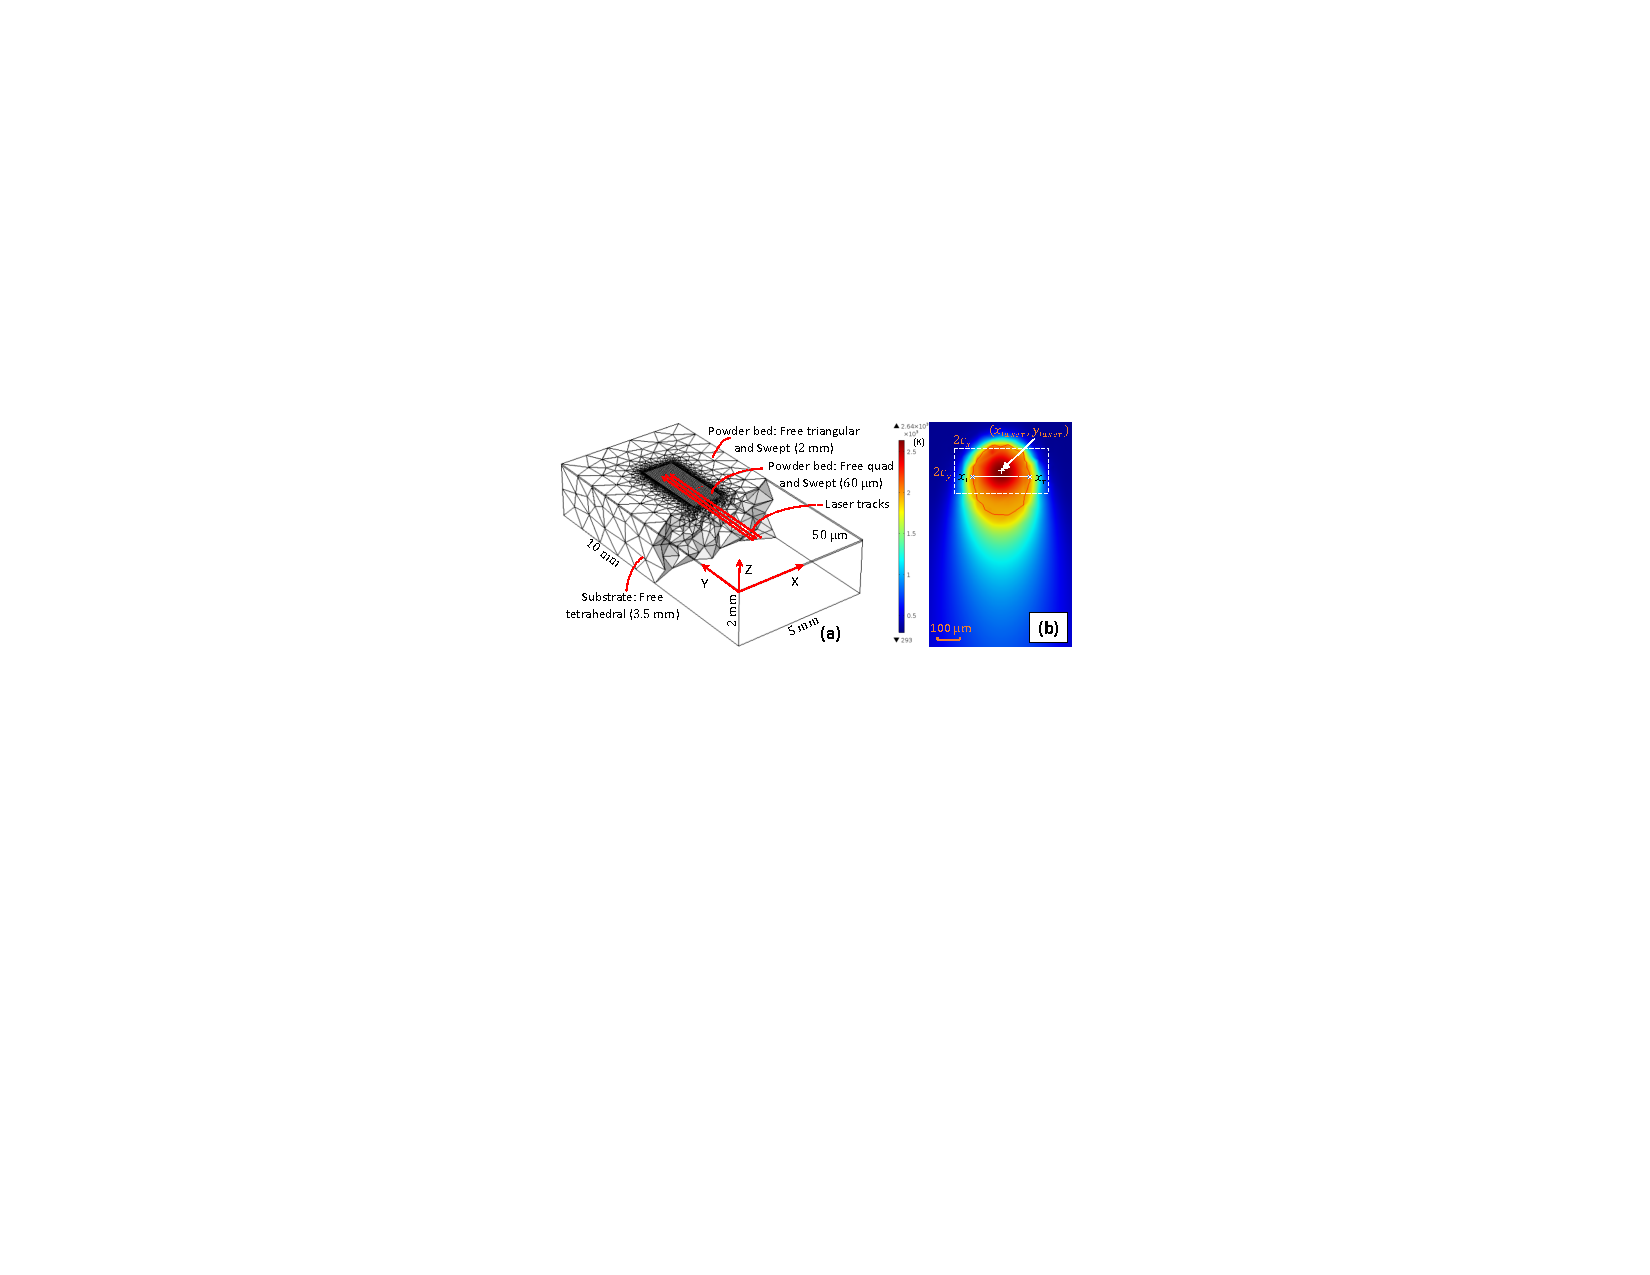
\includegraphics[clip,width=13cm]{Closed-loop-simulation/mesh_temp_distri}
\par\end{centering}
\centering{}\caption{\label{fig:Mesh-and-scan}(a): a thin layer of powder bed and the
substrate with selective meshing scheme. (b): surface temperature
distribution at $t=0.14\,\text{s}$. The lined isotherm indicates
$T=T_{m}$.}
\end{figure}
From the FEM-predicted temperature distribution, Fig. \ref{fig:Pseudocode-for-calculating}
shows the pseudocode of how to calculate the melt pool width. The
basic principle is to search around the position of the laser beam
to find the maximum width of the melt pool bounded by $T_{m}$. The
first step is to locate the position of the laser beam $(x_{laser},\,y_{laser})$,
as shown in Fig. \ref{fig:Mesh-and-scan}b. Then we identify the points
to traverse by testing and ensuring that the rectangle $2c_{x}\times2c_{y}$
be inclusive of anticipated melt pool widths (Fig. \ref{fig:Mesh-and-scan}b).
A set $X$ stores the $x$ coordinates of these points with an increment
$\Delta x$, and a set $Y$ stores the $y$ coordinates with $\Delta y$.
For each $y$ in $Y$, we search in $X$ to find the left boundary
$x_{l}$ and right boundary $x_{r}$ that have the temperature of
$T_{m}$. A width $w_{y}$ for a certain $y$ is given by $x_{r}-x_{l}$.
After going over all the points, we identify the melt pool width as
the maximum $w_{y}$. In this study, we choose $\Delta x=\Delta y=1\,$$\muup$m,
$c_{x}=150\,$$\muup$m, and $c_{y}=100\,$$\muup$m.
\begin{figure}[!ht]
\begin{centering}
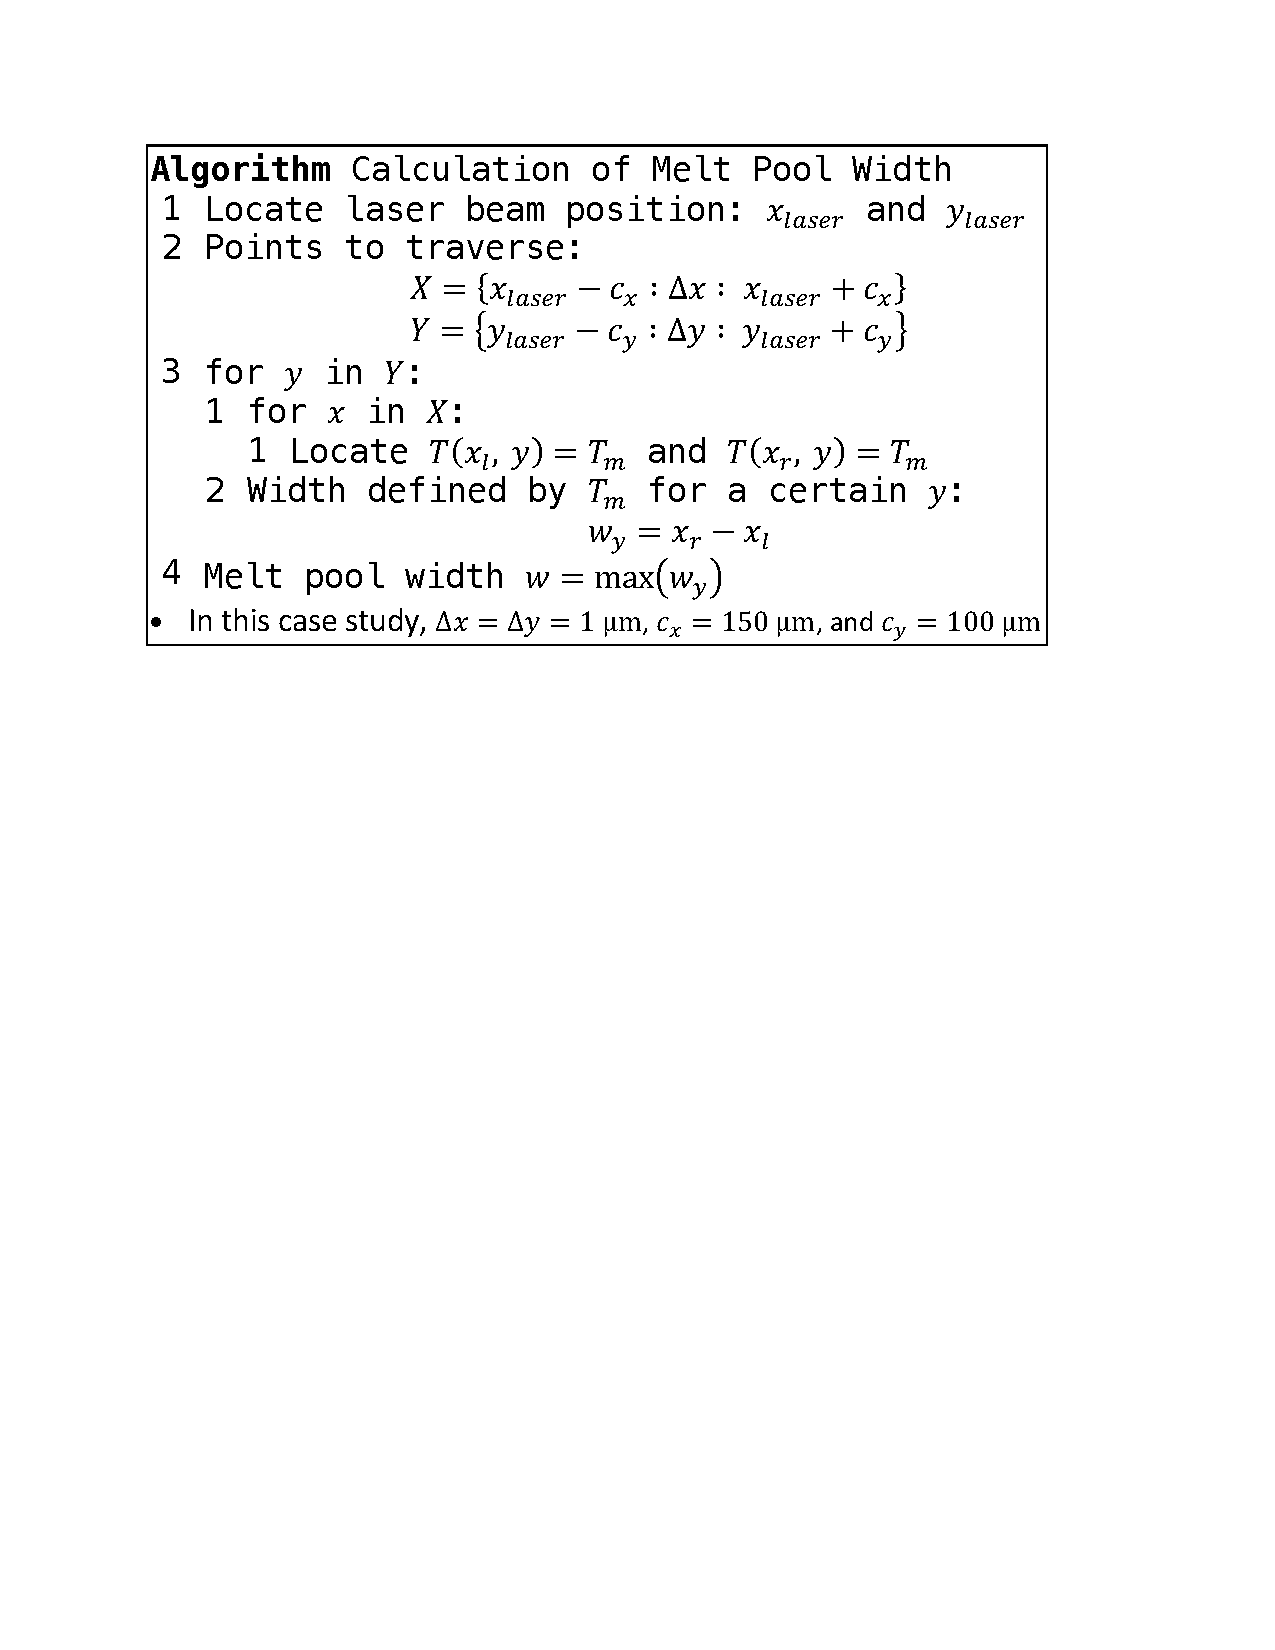
\includegraphics[clip,width=10cm]{Closed-loop-simulation/pseudocode_mpw}
\par\end{centering}
\centering{}\caption{\label{fig:Pseudocode-for-calculating}Pseudocode for calculating
melt pool width.}
\end{figure}

\section{Model Verification} \label{sec:Model-Verification}

\begin{table}[!ht]
\caption{\label{tab:Model-verification:-comparing}Melt pool widths from FEM
and experimental results with a fixed
laser power of 50 W and different scan speeds. Difference (Diff.)=FEM-Experiments
(Exper.). Error=|FEM-Exper.|/FEM.}

\centering{}\renewcommand{\arraystretch}{1}\begingroup\tabcolsep=1pt%
\begin{tabular*}{10cm}{@{\extracolsep{\fill}}ccccc}
\hline 
Scan speed & FEM($\muup$m) & Exper. ($\muup$m) & Diff. ($\muup$m) & Error (\%)\tabularnewline
\hline 
100 mm/s & 182 & 165.7$\sim$175.4 & 6.6$\sim$16.3 & 3.6$\sim$9.0\tabularnewline
200 mm/s & 152.6 & 140.7$\sim$142.9 & 9.7$\sim$11.9 & 6.4$\sim$7.8\tabularnewline
300 mm/s & 132.6 & 120.7$\sim$125.4 & 7.2$\sim$11.9 & 5.4$\sim$9.0\tabularnewline
\hline 
\end{tabular*}\endgroup
\end{table}
This section verifies the developed FEM by comparing the numerical
melt pool widths with the experimental and analytical solutions.
Table \ref{tab:Model-verification:-comparing} first compares the
melt pool widths obtained from the developed FEM with the experimental
results in \cite{yadroitsev2014selective}. The laser power is fixed
to be $50\,\text{W}$, the laser spot diameter is $70\,$$\muup$m,
and the scan speed is 100, 200, or $300\,\text{mm/s}$. The FEM gives
reasonable predictions of the melt pool widths with errors less than
10\%.

Then we compare the numerical melt pool widths with the analytical
solutions. When a moving point laser source is acting on a thick plate
and the thermal properties of the plate are constant, the analytical
solution of (\ref{eq:heat_conduction}) in the steady state is the
Rosenthal equation \cite{kannatey2009principles}:

\noindent 
\begin{equation}
T(\xi,\,y,\,z)-T_{0}=\frac{q}{2\pi kr}\text{e}^{-\frac{u_{x}(r+\xi)}{2\kappa}},\label{eq:Rosenthal}
\end{equation}

\noindent where $(\xi,\,y,\,z)$ is a coordinate system attached to
the moving laser source, $r=\sqrt{\xi^{2}+y^{2}+z^{2}}$, and $\kappa=k/(\rho c_{p})$.
For comparison, we adapt the FEM to accommodate the assumptions of
the Rosenthal equation, such as constant thermal properties ($k=5\:\text{W/(m}\cdotp\text{K)}$,
$c_{p}=1.1\:\text{J/(g}\cdotp\text{K)}$, and $\rho=4300\:\text{kg/m}^{3}$)
and point heat source. Fig. \ref{fig:Model-verification:-comparing}
compares the numerical and analytical solutions. From Fig. \ref{fig:Model-verification:-comparing}a,
we can tell that the melt pool widths obtained from the FEM and the
Rosenthal equation match well with each other under different combinations
of scan speeds and laser powers. Also, as shown in Figs. \ref{fig:Model-verification:-comparing}b
and \ref{fig:Model-verification:-comparing}c, after 27 samples, the
numerical melt pool geometry reaches to the steady state and matches
with the Rosenthal solution (the outline). 
\begin{figure}[!ht]
\begin{centering}
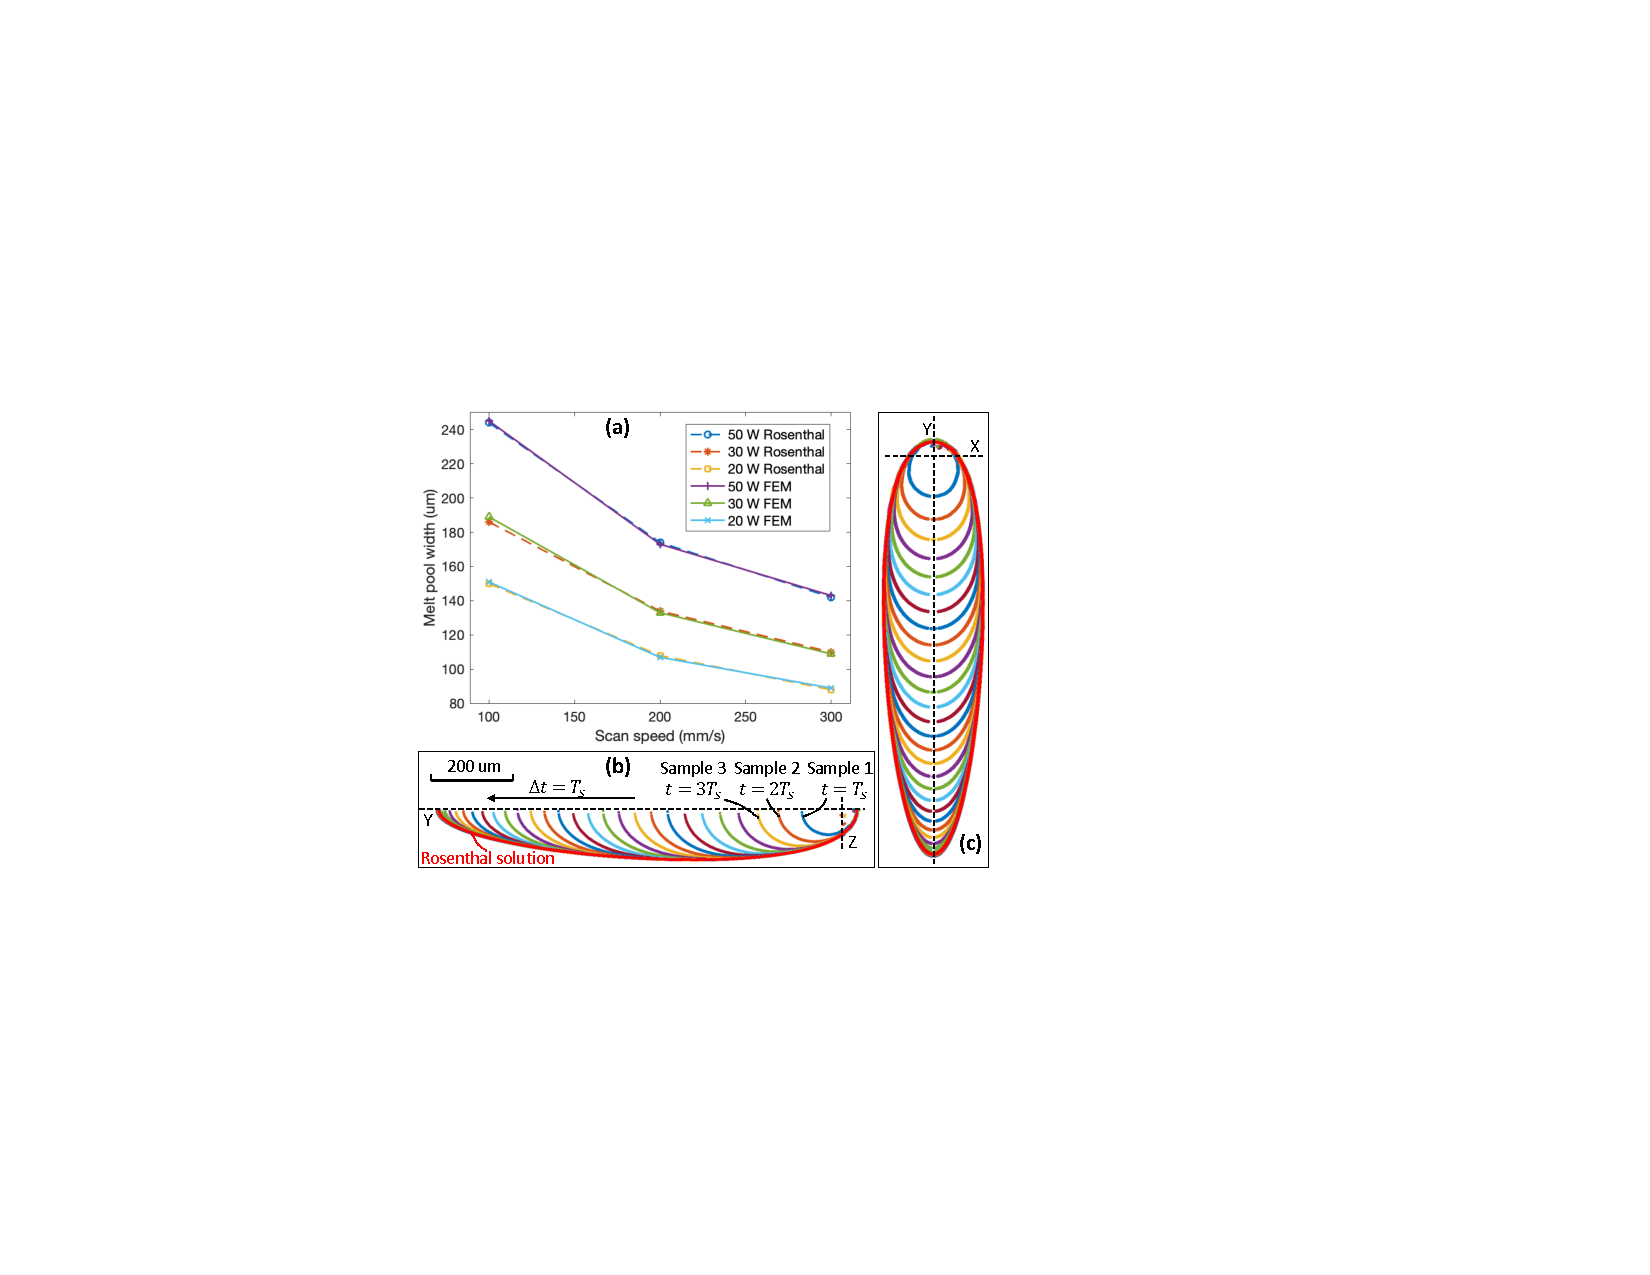
\includegraphics[clip,width=12cm]{Closed-loop-simulation/model_verification_rosenthal}
\par\end{centering}
\centering{}\caption{\label{fig:Model-verification:-comparing}Melt pool widths from the
FEM and analytical solutions. (b) and (c) share the same scale and
legend.}
\end{figure}

\section{Periodic Thermal Interactions} \label{sec:Periodic-Thermal-Interactions}

We adopt the verified FEM in Section \ref{sec:FEM} to investigate the periodic
LPBF thermal cycles and will then design a repetitive controller to regulate these cycles in Chapter \ref{chap:RC-Closed-loop-Simulation}.

\subsection{Periodic Thermal Interactions: Hatch Spacing} \label{subsec:Hatch-Spacing}

We first examine how hatch spacing affects the melt pool variation,
especially during the transition from the end of one track (named
P1) to the start of the adjacent track to be sintered (P2). Here,
hatch spacing is defined as the distance between two adjacent scan
vectors and denoted as $\Delta x$ in Fig. \ref{fig:Schematic-of-in-layer}.
When the hatch spacing (e.g., $47\,$$\muup$m in (a1)-(a4) of Fig.
\ref{fig:Melt-pool-variation}) is much less than half of the melt
pool width (around the laser spot radius $110\,$$\muup$m), the laser
spot at P2 will be centered inside the melt pool region of P1 and
thus can take advantage of the accumulated heat, yielding a well-developed
melt pool at $50.5\,\text{ms}$. When the hatch spacing (e.g., $100\,$$\muup$m
in (b1)-(b4) of Fig. \ref{fig:Melt-pool-variation}) is close to or
larger than half of the melt pool width, the laser spot at P2 will
be centered out of the melt pool region of P1, yielding a lower initial
temperature at P2. Besides, since the laser is turned off during the
transition, a larger hatch spacing ($100\,$$\muup$m) gives a longer
dwell time ($1\,\text{ms}$) with the same scan speed ($100\,\text{mm/s}$).
Hence, previously fused tracks would have more time to cool down,
which also yields a lower initial temperature at P2. Therefore, the
melt pool evolves slower at P2, and two immature states show up at
$550.5\,\text{ms}$ and $551\,\text{ms}$, which will cause more porosity
in the printed part. 

To get consistent part quality in LPBF, a stable melt pool is desired
during the transition. The immature melt pool states can be eliminated
by decreasing the hatch spacing. However, there is a trade-off between
melt pool stability and printing efficiency since simply shortening
the hatch spacing increases printing time. Next we will study periodic
melt pool variations that are intrinsic in the LPBF process and demand
much more involved solutions, such as advanced control algorithms.
\begin{figure}[!ht]
\begin{centering}
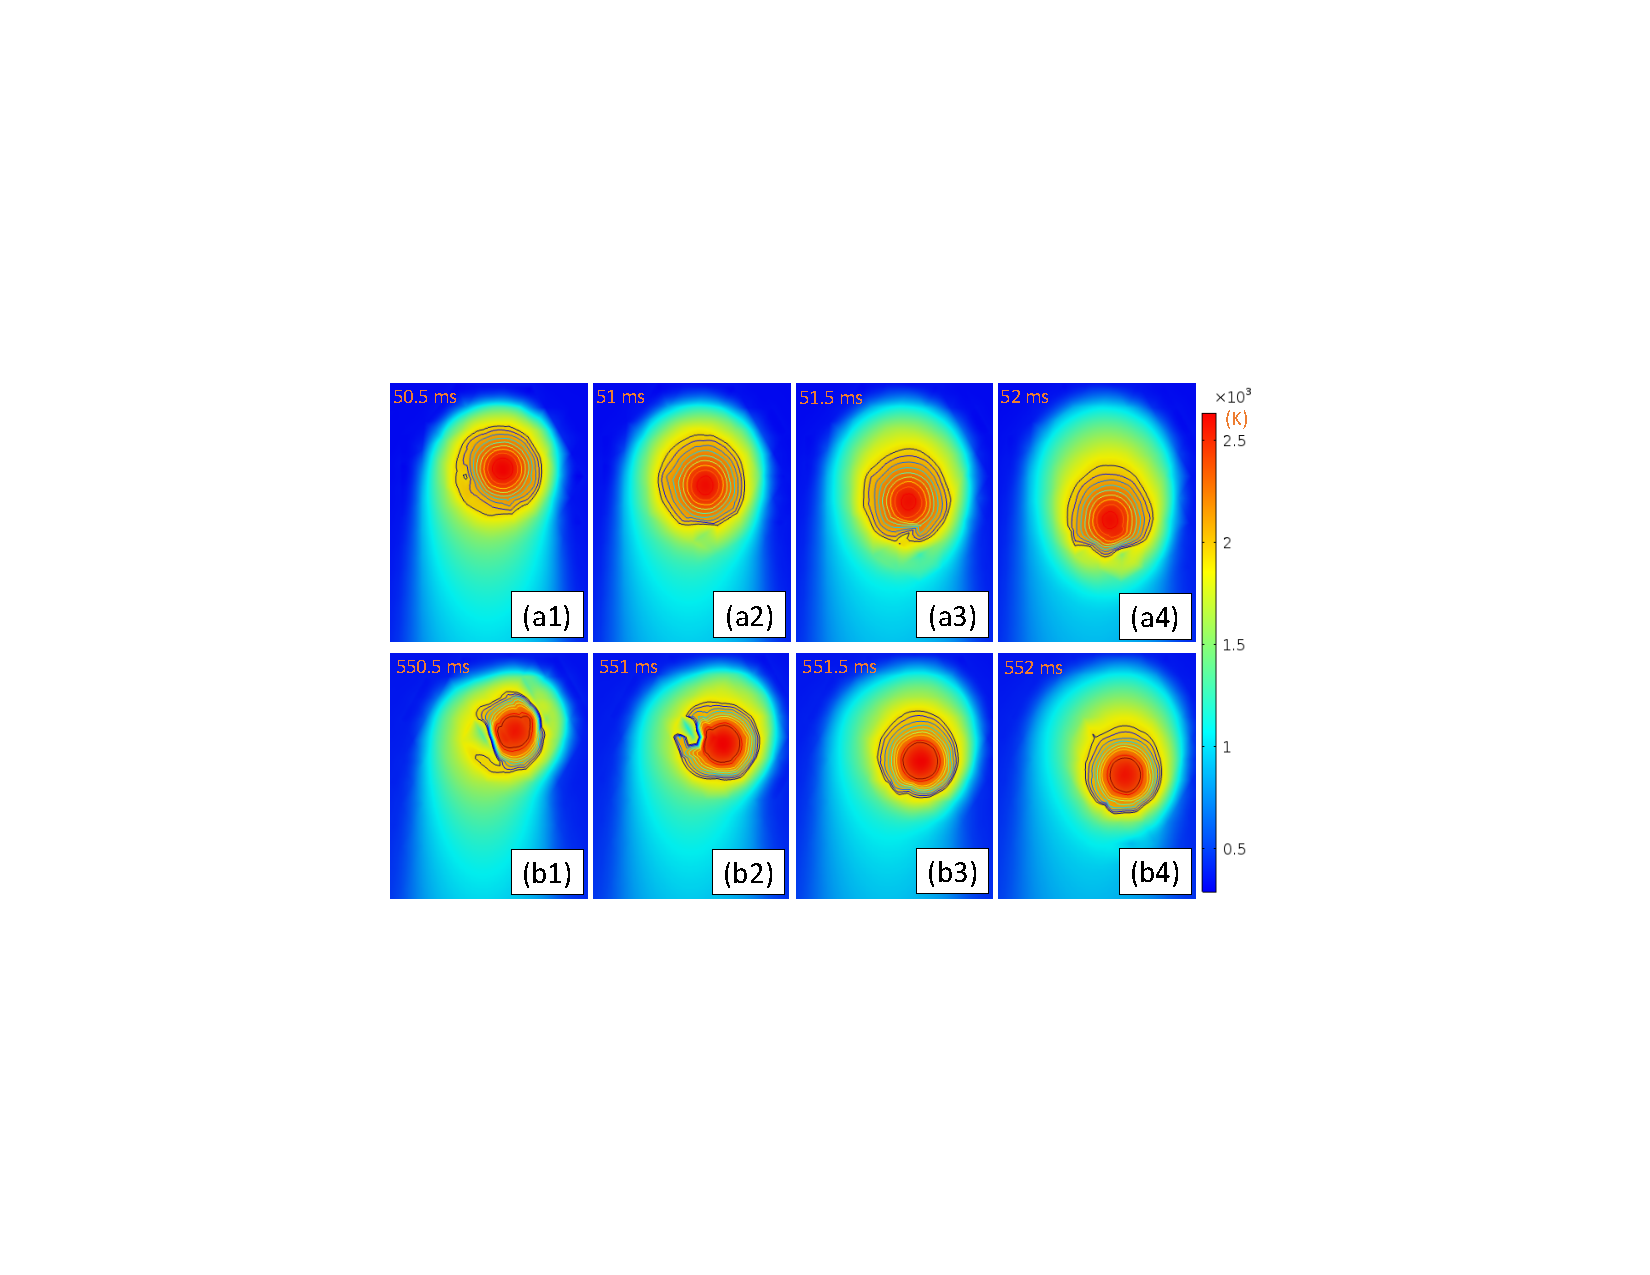
\includegraphics[clip,width=13cm]{Closed-loop-simulation/hatchspacing_smalllarge}
\par\end{centering}
\centering{}\caption{\label{fig:Melt-pool-variation}Melt pool variations at the start
of the 2nd track with hatch spacing of $47\,$$\muup$m (i.e., dwell
time of 0.47 ms) in (a1)-(a4) and the start of the 12th track with
hatch spacing of $100\,$$\muup$m (i.e., dwell time of 1 ms) in (b1)-(b4).}
\end{figure}

\subsection{Periodic Thermal Interactions: In-layer Effects} \label{subsec:In-layer-Effects}

\begin{figure}[!ht]
\begin{centering}
\subfloat[\label{fig:Evolution-of-melt-2}Evolution of melt pool width (time-domain)]{\begin{centering}
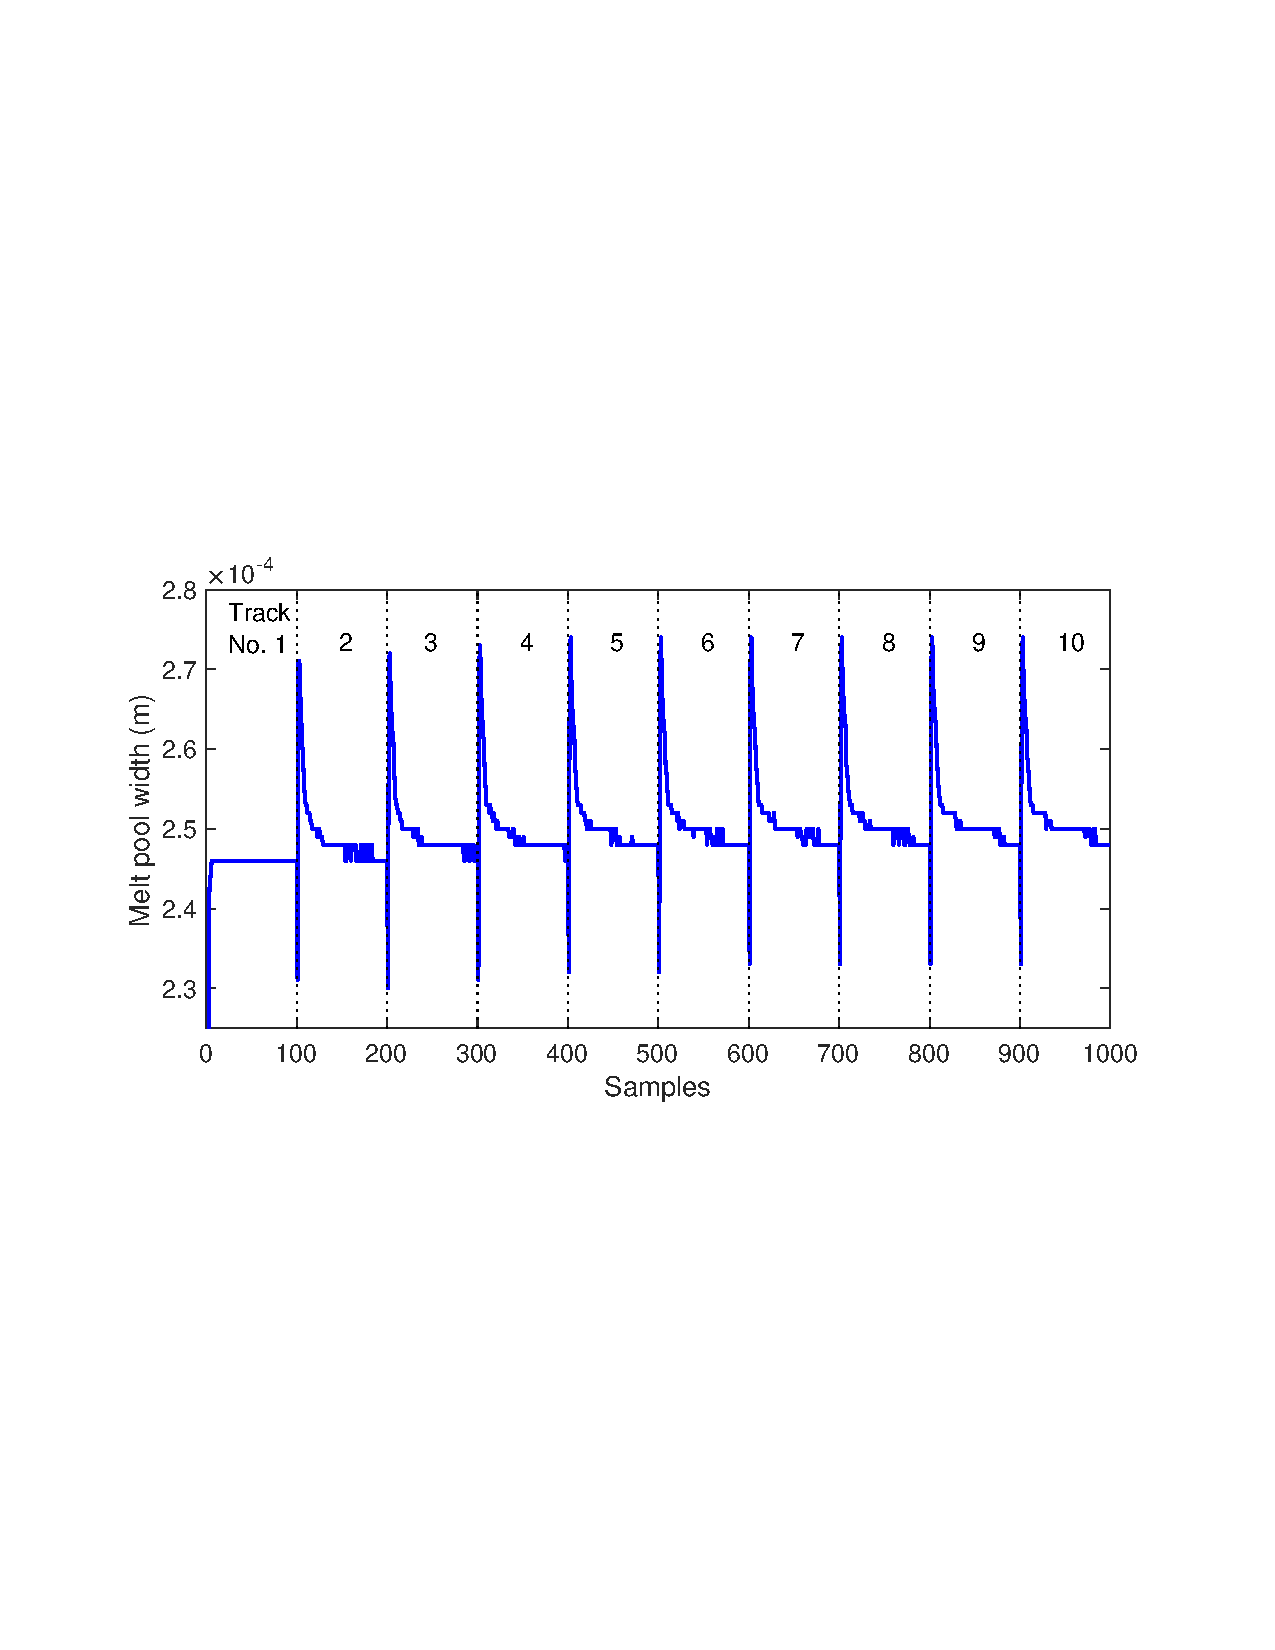
\includegraphics[clip,width=12cm]{Closed-loop-simulation/mpw_straight_20Hz_cnstq_2_time}
\par\end{centering}
}
\par\end{centering}
\begin{centering}
\subfloat[\label{fig:FFT-of-melt-pool-width-2}FFT of melt-pool-width evolution
(frequency-domain)]{\begin{centering}
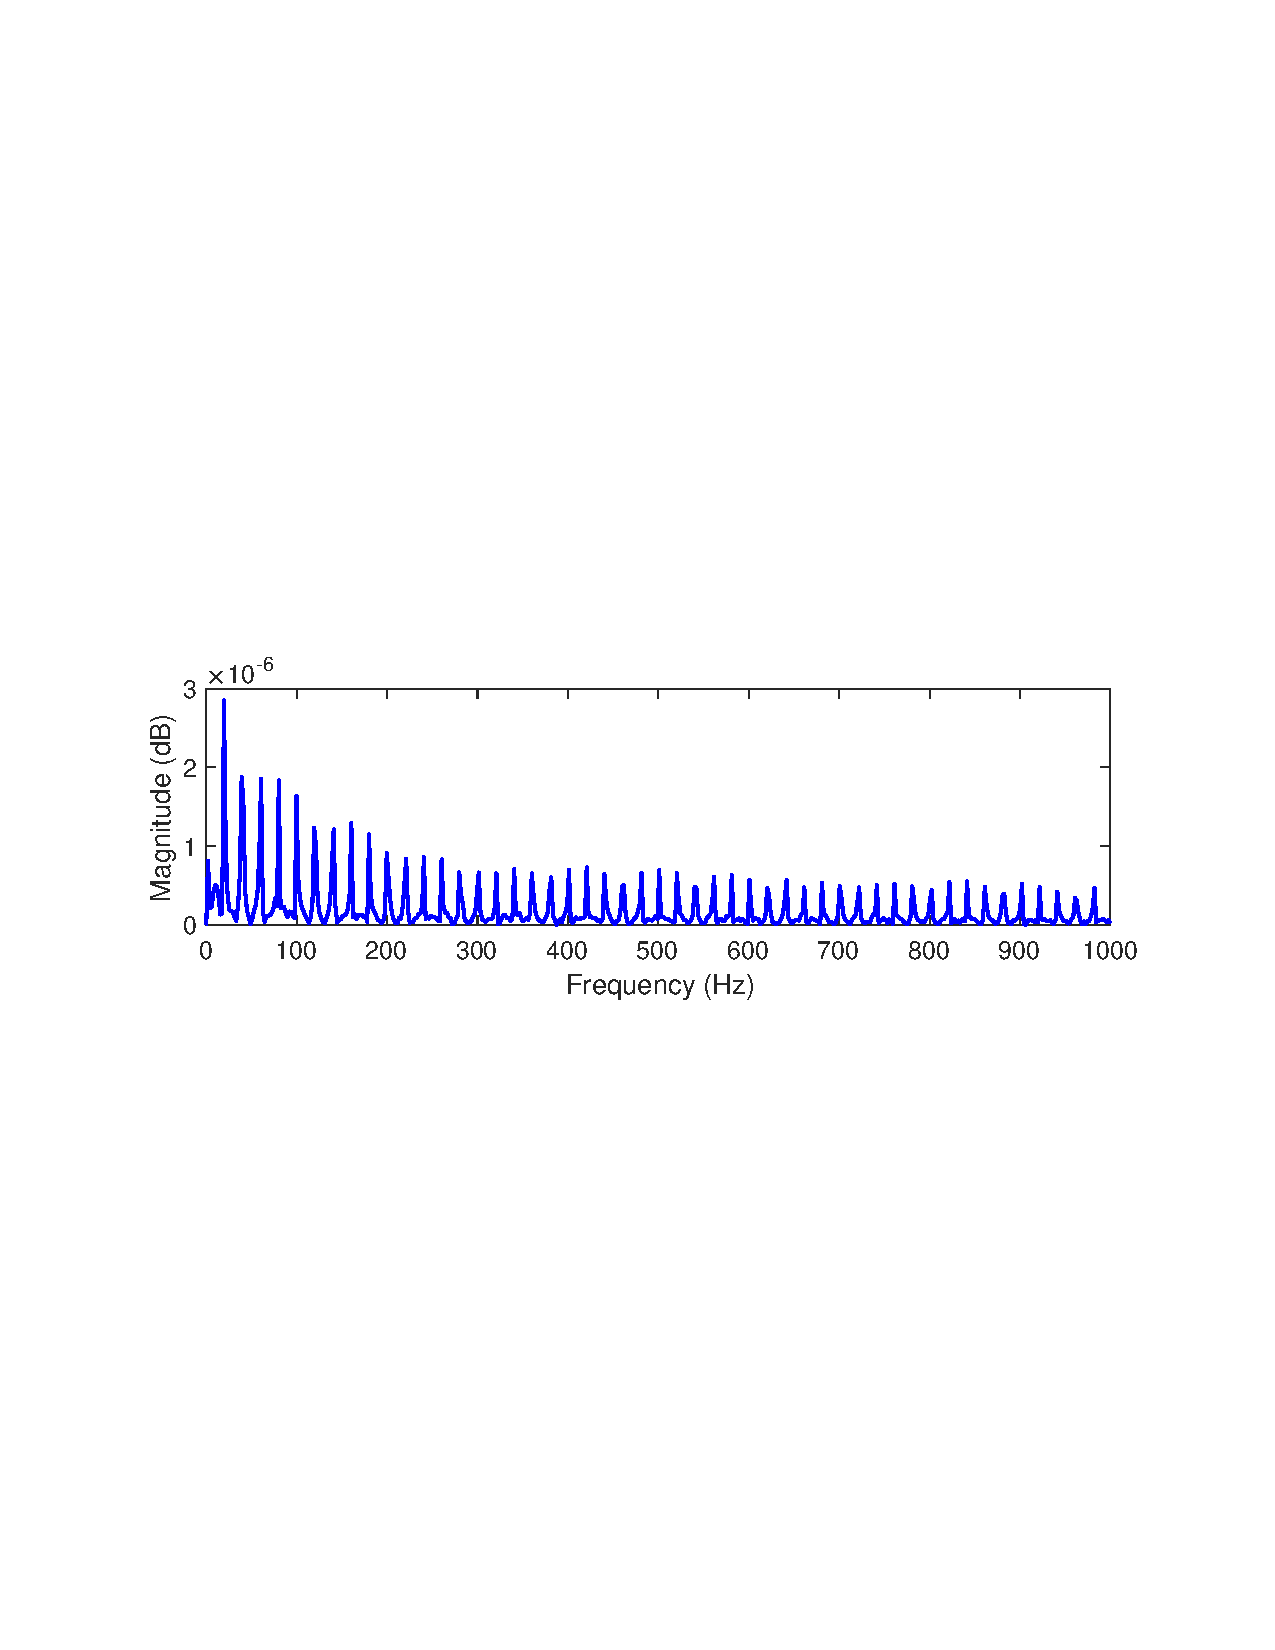
\includegraphics[clip,width=12cm]{Closed-loop-simulation/mpw_straight_cnstq_freq_onefig_2}
\par\end{centering}
}
\par\end{centering}
\centering{}\caption{\label{fig:In-layer-melt-pool-1}In-layer thermal disturbance with
constant laser power.}
\end{figure}
To investigate the in-layer thermal cycles, we bidirectionally print
10 tracks in the first layer with a hatch spacing of $60\,$$\muup$m
(Fig. \ref{fig:Mesh-and-scan}a). From Fig. \ref{fig:Evolution-of-melt-2}, we observe that the melt pool
width changes over time and structurally deviates from the steady-state
value $246\,$$\muup$m as extracted from the first track. Most importantly,
the start of each track has larger melt pool widths than the rest
of the track. This is because in bidirectional scanning, when the
energy beam approaches the end of one track, the large latent heat
does not have enough time to dissipate out before the next track starts.
The resulting increased melt pool widths at the beginning of each
track form a periodic disturbance with a repetitive spectrum in the
frequency domain (Fig. \ref{fig:FFT-of-melt-pool-width-2}). The fundamental
frequency $f_{0}$ of the disturbance is determined by the duration
of scanning one track $t_{0}$, that is, $f_{0}=1/t_{0}=u_{x}/L$,
where $u_{x}$ is the scan speed and $L$ is the track length. In
this example, $f_{0}=100/5=20\,\text{Hz}$, and frequency spikes at
${nf_{0}}\,$($n\in\mathbb{Z}^{+}$, the set of positive integers)
appear in the fast Fourier transform (FFT) of the disturbance.

The disturbance periodicity is closely related to the recurring laser
scanning trajectories and the repetitive in-layer thermomechanical
interactions. Besides the bidirectional scan, other scan patterns
yield similar repetitive disturbances (see, e.g., experimental results
in \cite{dunbar2017comparisons}). To deal with these undesired repetitive
spectra, we develop the closed-loop simulation in Chapter \ref{chap:Closed-loop-Simulation}
to bring automatic control algorithms \cite{chen2014new,wang2018multirate}
into FEM. More results and analyses will be elaborated in Part
\ref{part:Multirate-Feedback-Control}.

\subsection{Periodic Thermal Interactions: Combined In- and Cross-layer Effect} \label{subsec:In-and Cross-layer-Effects}

\begin{figure}[!ht]
\begin{centering}
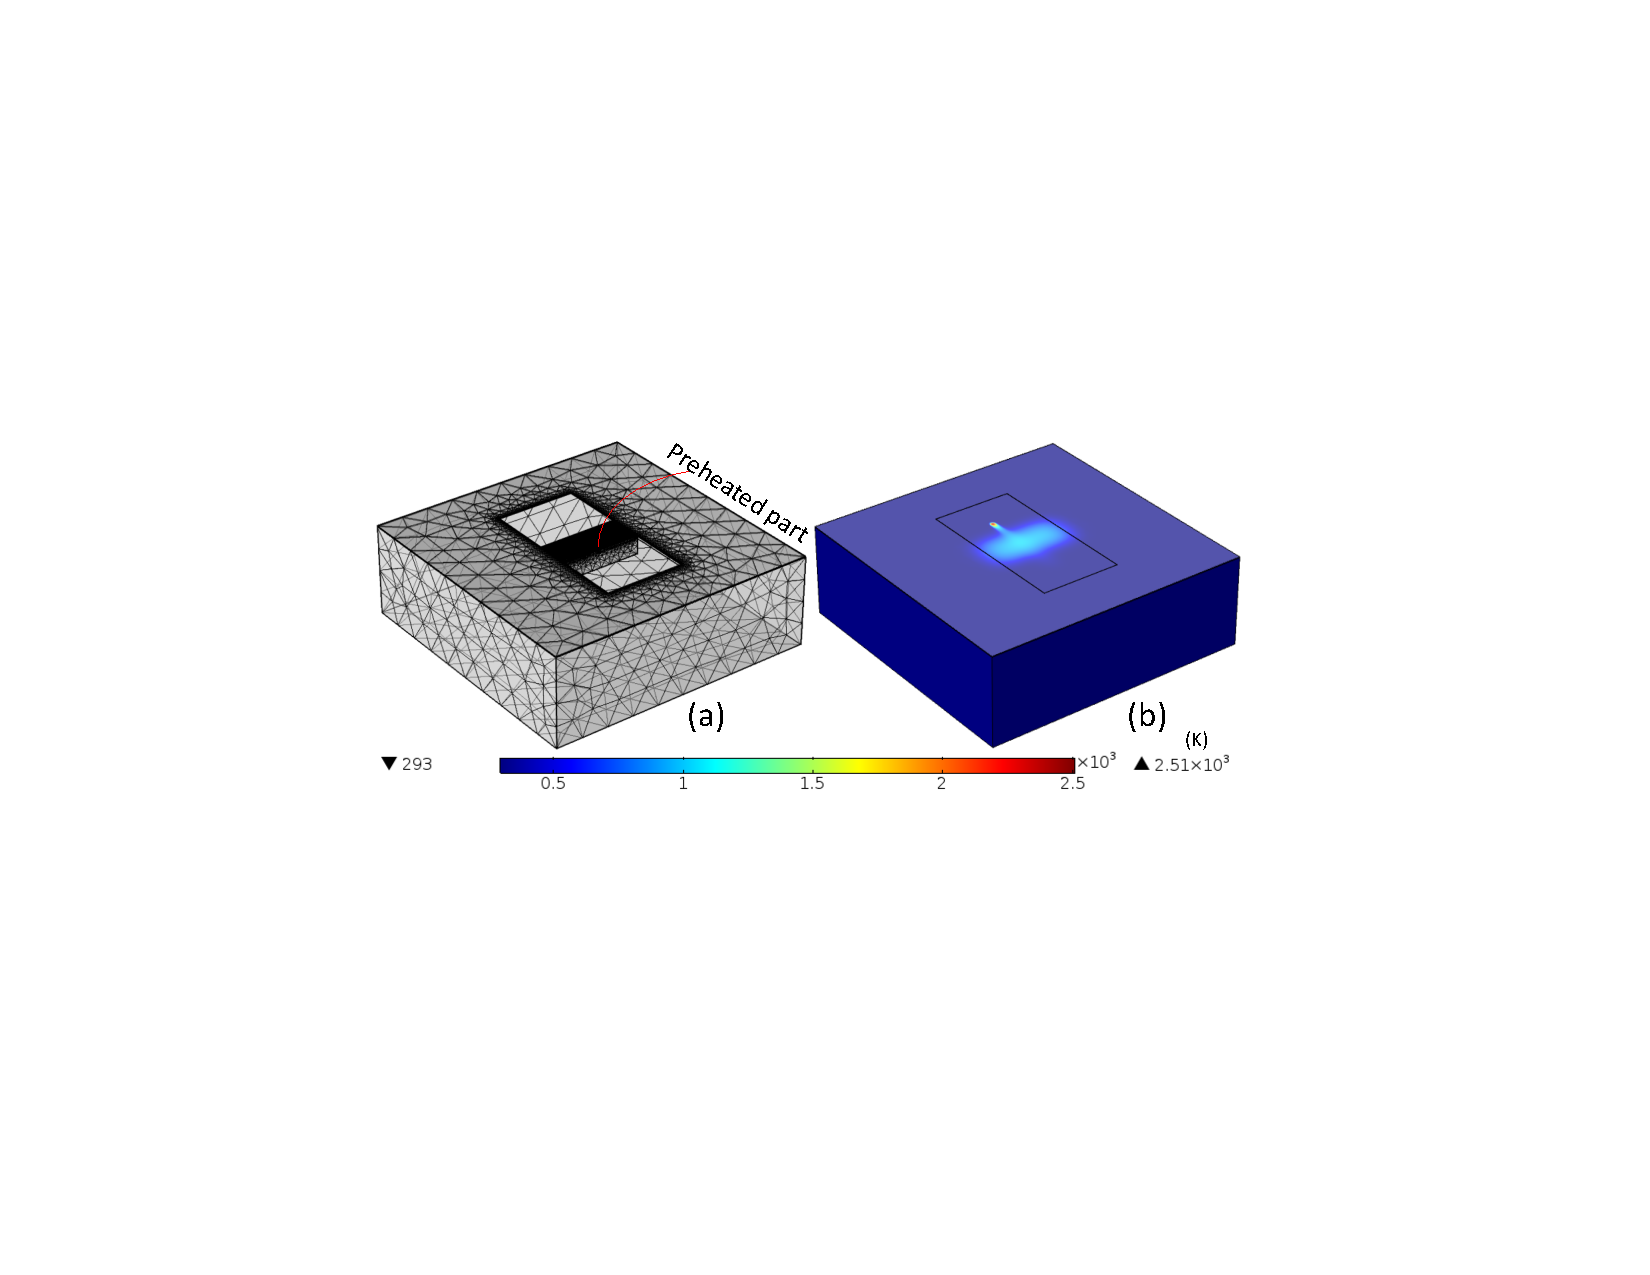
\includegraphics[clip,width=13cm]{Closed-loop-simulation/crosslayer_tem_mesh}
\par\end{centering}
\begin{centering}
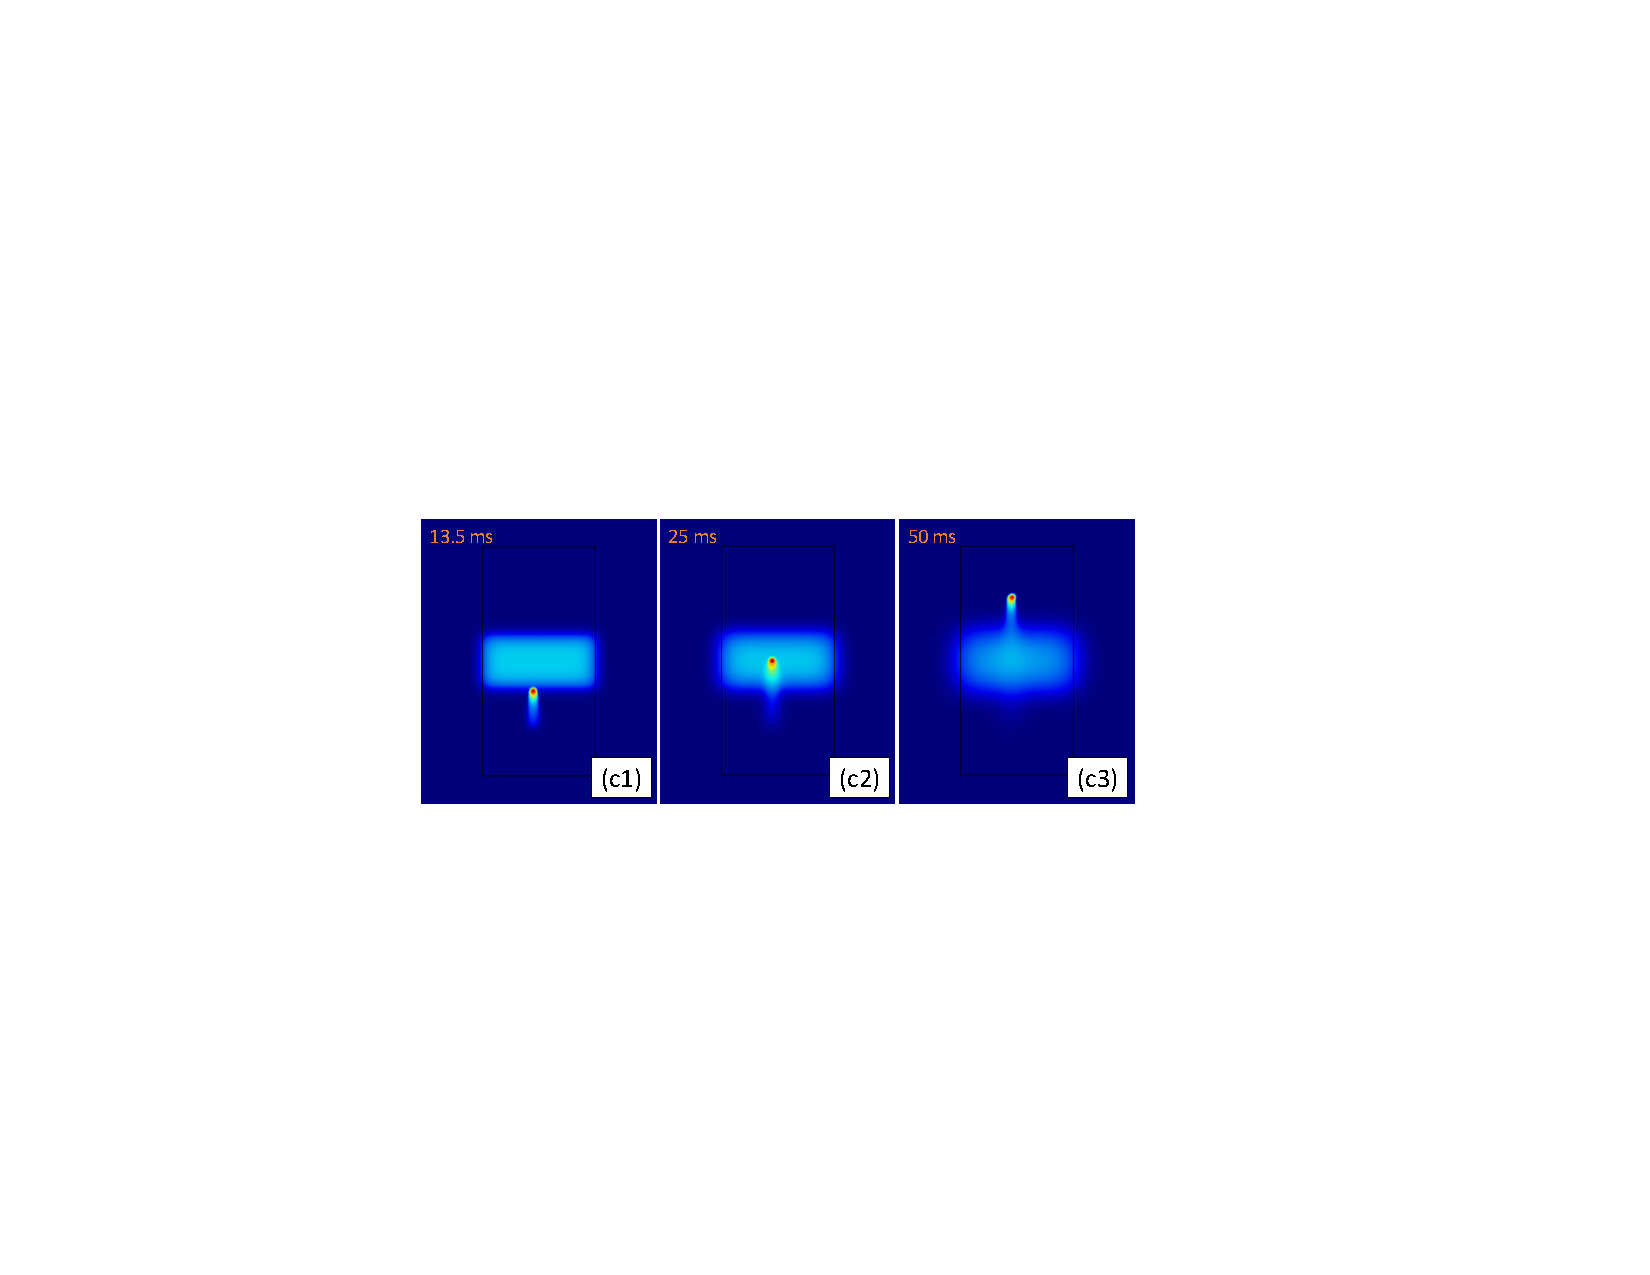
\includegraphics[clip,width=13cm]{Closed-loop-simulation/crosslayer_three}
\par\end{centering}
\centering{}\caption{\label{fig:Mesh-with-added}(a): mesh with added preheated part. (The
thin layer of powder bed is hidden to unveil the added part.) (b):
surface temperature distribution at $t=49\,\text{ms}$. (c1)-(c3):
surface temperature distributions (top view) during the printing of
the first track.}
\end{figure}
This section demonstrates the combined effect of periodic in- and
cross-layer thermal interactions. As shown in Fig. \ref{fig:Mesh-with-added},
we put under the powder bed a Ti6Al4V part ($4.45\times1\times1\,\text{mm}^{3}$)
that is preheated to $1200\,\text{K}$ \cite{liu2019additive}. Due
to the high initial temperature of the added part, the powder on top
of the part has a higher initial temperature than the powder elsewhere.
The scan strategy is the same as that in Fig. \ref{fig:Mesh-and-scan}a.
Eight tracks are scanned bidirectionally with the hatch spacing of
$50\,$$\muup$m. The length of the laser track ($5\,\text{mm}$)
is greater than that of the added part ($1\,\text{mm}$). This configuration
imitates the printing process of parts with overhang structures, where
the preheated Ti6Al4V part corresponds to the previously fused layers.
As in Fig. \ref{fig:Mesh-and-scan}, we also use the selective mesh
scheme (Fig. \ref{fig:Mesh-with-added}a): triangular-and-swept ($72.6\,$$\muup$m)
for the central powder bed, triangular-and-swept ($1.5\,\text{mm}$)
for the peripheral powder bed, and free tetrahedra ($2\,\text{mm}$)
for the substrate and the added part.

In Fig. \ref{fig:Mesh-with-added}, plots (c1)-(c3) illustrate the
top views of the surface temperature profiles during the first-track
printing from 0 to $50\,\text{ms}$. When the laser is passing over
the preheated powder at $25\,\text{ms}$, we get a larger melt pool
width, compared to when the laser is approaching ($t=13.5\,\text{ms}$)
or leaving ($t=50\,\text{ms}$) the preheated region. The larger melt
pool width is generated due to the higher initial temperature of powder
on top of the preheated part.

During the evolution of the melt pool width in Fig. \ref{fig:Evolution-of-melt},
at the beginning of each track, there is a large increase of the melt
pool width caused by the in-layer thermal interaction, as explained
in Section \ref{subsec:In-layer-Effects}. Besides, as indicated
by the arrows in Fig. \ref{fig:Evolution-of-melt}, larger melt pool
widths appear every time the laser passes over the powder on top of
the preheated part. These arrowed peaks caused by the cross-layer
thermal interaction get smaller as the heat accumulated by the preheated
part dissipates out (Tracks 7 and 8 in Fig. \ref{fig:Evolution-of-melt}).
This phenomenon can also be seen from the blurrier border of the preheated
region at $t=50\,\text{ms}$ in Fig. \ref{fig:Mesh-with-added} (c3).

\begin{figure}[!ht]
\begin{centering}
\subfloat[\label{fig:Evolution-of-melt}Evolution of melt pool width (time-domain).
An interval between two adjacent dashed lines indicates the printing
of one track, whereas inside one track, the interval between two adjacent
dotted lines denotes when the laser is passing over the preheated
part. ]{\begin{centering}
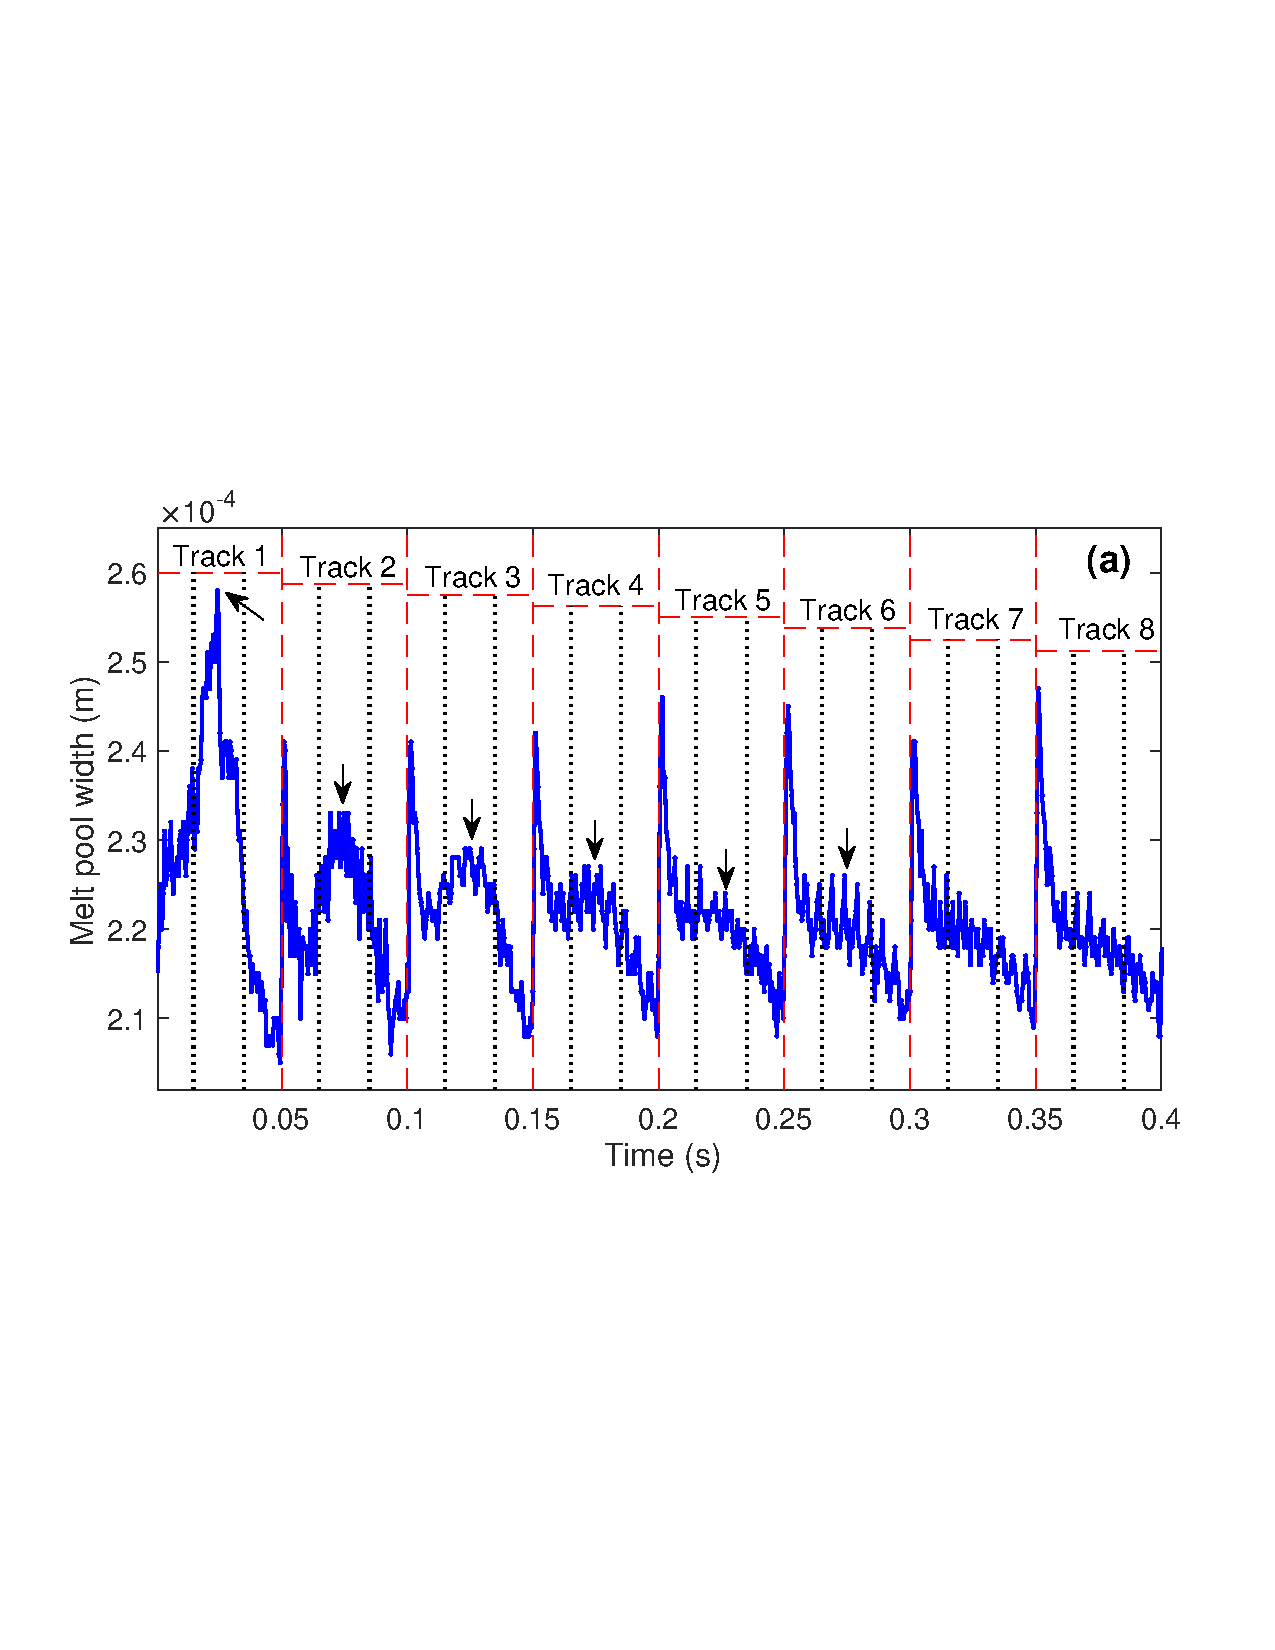
\includegraphics[clip,width=12cm]{Closed-loop-simulation/inandcrosslayerMPW}
\par\end{centering}
}
\par\end{centering}
\begin{centering}
\subfloat[\label{fig:FFT-of-melt-pool-width}FFT of melt-pool-width evolution
(frequency-domain)]{\begin{centering}
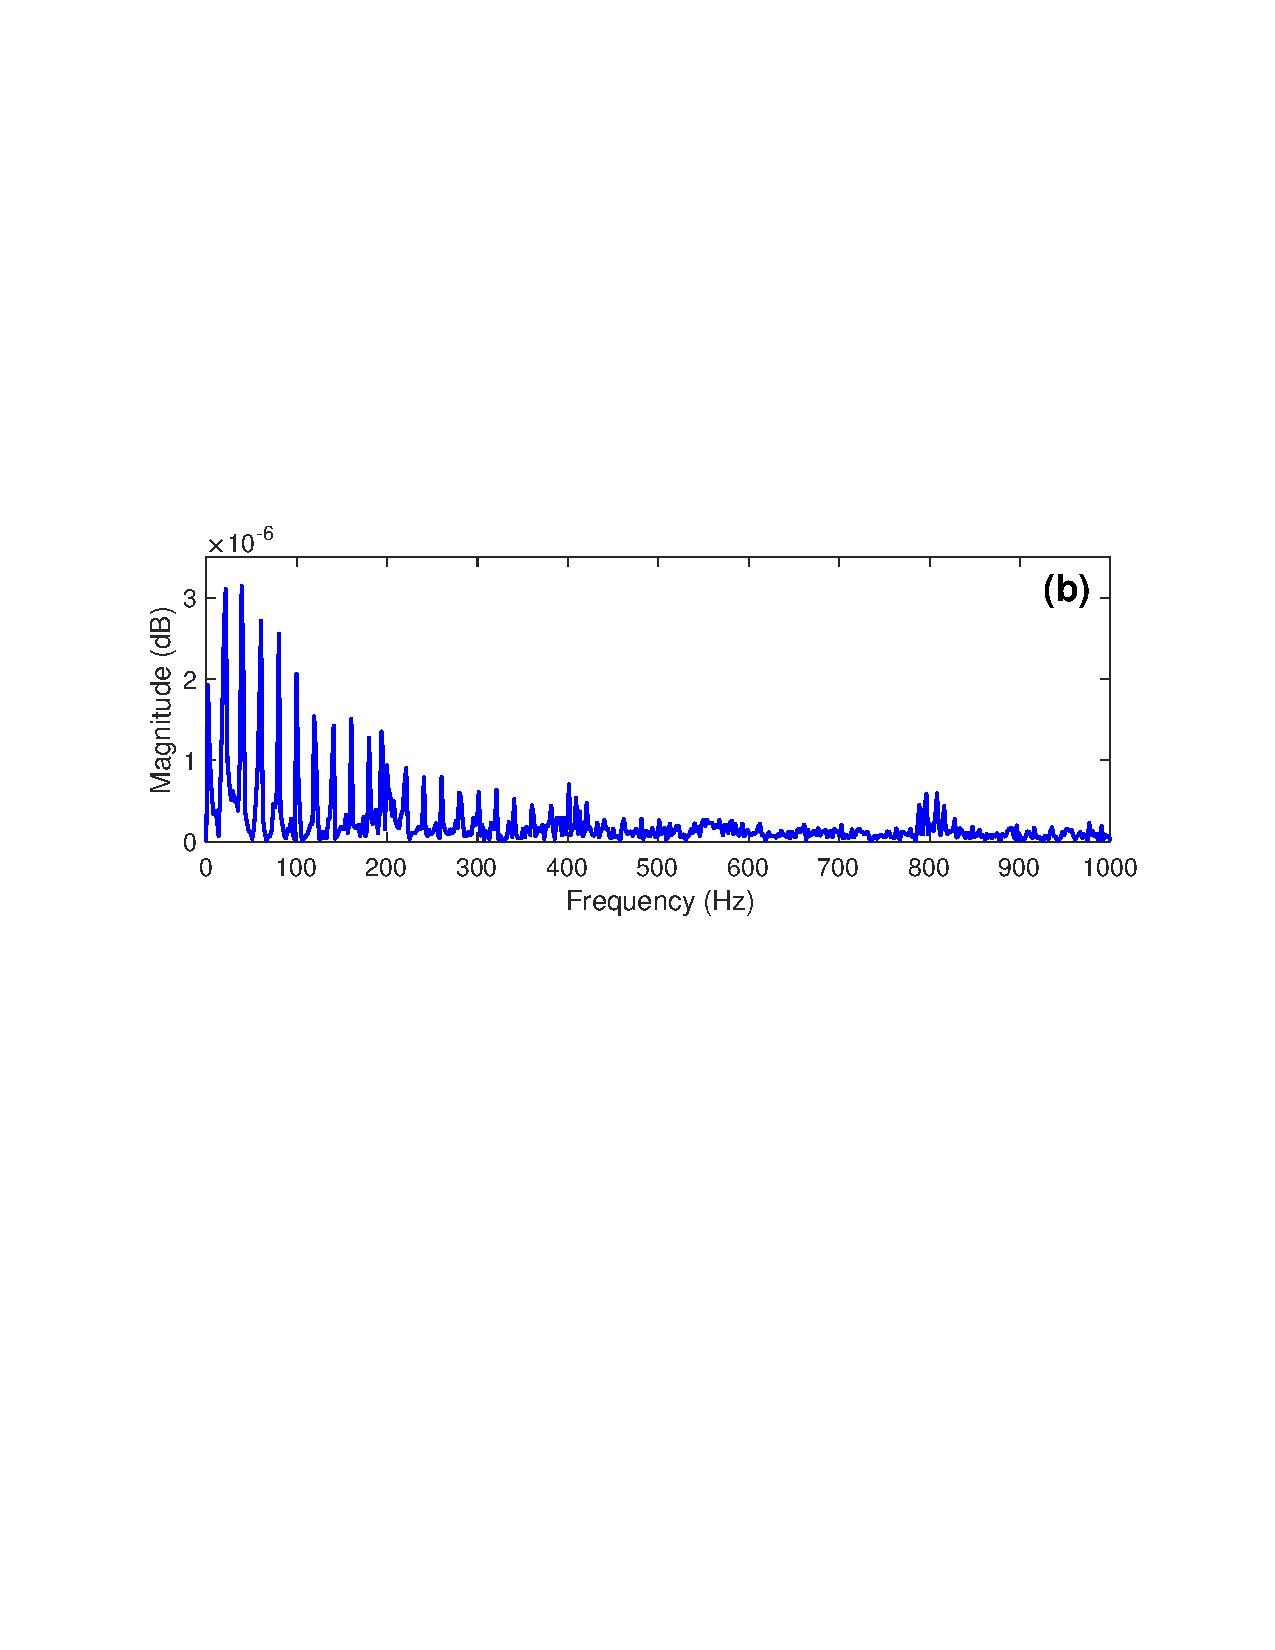
\includegraphics[clip,width=12cm]{Closed-loop-simulation/crosslayer_1200K}
\par\end{centering}
}
\par\end{centering}
\centering{}\caption{\label{fig:In-cross-layer-melt-pool}Combined in- and cross-layer
thermal disturbance. }
\end{figure}
We have demonstrated that the periodic evolution of the melt pool
width is a lumped output of the repetitive in- and cross-layer heat
transfer dynamics. When comparing the frequency spectra in Figs. \ref{fig:FFT-of-melt-pool-width-2}
and \ref{fig:FFT-of-melt-pool-width}, we can tell that the cross-layer
thermal interaction changes the magnitudes of the spectral peaks but
not the harmonic frequency values. These variations can thus be attenuated
by the same feedback control algorithms, such as the RC algorithm
to be introduced in Part \ref{part:Multirate-Feedback-Control}.


% ========== Chapter 4

\chapter{New Hammerstein Modeling} \label{chap:New-Hammerstein-Modeling}

\section{Introduction}

Appropriate modeling of this sophisticated
dynamic system plays a fundamental role in understanding and regulating
the LPBF and LPBF-related techniques such as LMD. This chapter establishes a new modeling and understanding of LPBF by
taking advantage of the FEM and control-oriented modeling. The FEM developed in Chapter \ref{chap:FEM} serves as a simulation platform to provide data for verifying and identifying
parameters of the proposed modeling schemes. In the control-oriented
modeling of LPBF, stepping beyond commonly used low-order system models  \cite{kruth2007feedback,craeghs2010feedback,zheng2020distributed,song2011feedback,cao2015control,sammons2014repetitive}, this chapter develops a physics-based Hammerstein model that accommodates
more of the convoluted spatiotemporal thermomechanical dynamics. The
Hammerstein model is formulated by concatenating a memoryless nonlinear
submodel derived from the Rosenthal equation to a linear model obtained
from standard system identification techniques with laser power as
the input and melt pool width as the output. We verify the accuracy
of the Hammerstein model using the FEM and prove that the identified
model is only a linear representation of the Hammerstein model around
the equilibrium point. Along the way, we analyze the stability and
robustness properties of the models and present a generic control
scheme of the Hammerstein model.

In the remainder of this chapter, Section \ref{sec:ANALYTICAL-SOLUTIONS-AND}
identifies the linear plant model from the FEM. Section \ref{sec:HAMMERSTEIN-MODEL-IN}
derives the closed-form expressions of the steady-state melt pool
width and furthermore develops and analyzes the main Hammerstein model.

\section{\label{sec:ANALYTICAL-SOLUTIONS-AND}Linear Model}

From the FEM developed in Chapter \ref{chap:FEM}, we identify the linear plant model as $P(s)=0.001671/(s+1055)$
from laser power changes $\delta q$ to melt pool width changes $\delta w$
around the equilibrium point at ($q_{0}=60\,\text{W},\,$$w_{0}=248.41\,$\textmu m).
Here, $q=q_{0}+\delta q$ and $w=w_{0}+\delta w$ are the actual laser
power fed to the FEM and the melt pool width generated from the FEM,
respectively. The input signals fed to the FEM include a pseudorandom
binary sequence (PRBS) signal and multiple sinusoidal signals (10$\sim$300
Hz), with a magnitude of 20 W and an add-on DC component of $q_{0}=60\,\text{W}$.
\begin{figure}[!ht]
\begin{centering}
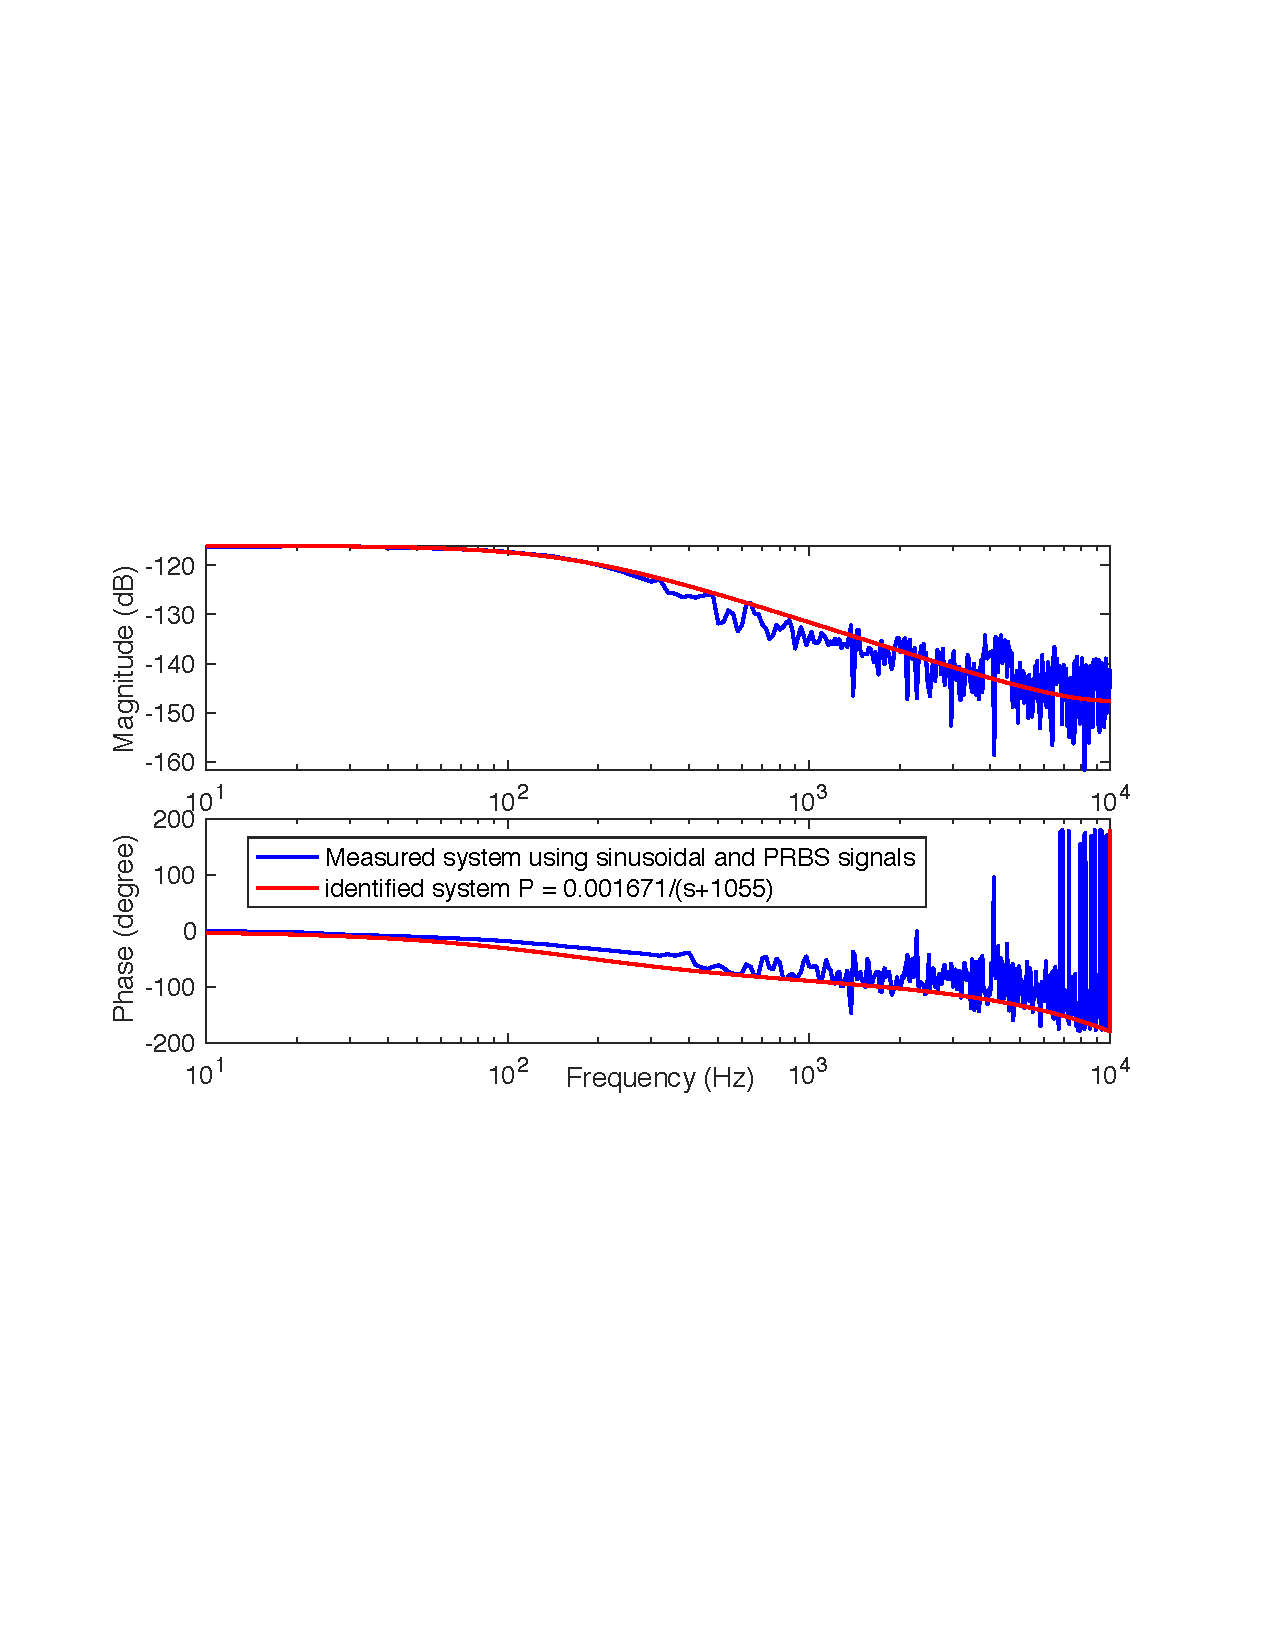
\includegraphics[clip,width=13cm]{Hammerstein/systemid_measured_identified_systems}
\par\end{centering}
\centering{}\caption{\label{fig:Measured-and-identified-H}Measured and identified system
responses.}
\end{figure}
The frequency responses of the measured and identified systems match
well with each other (Fig. \ref{fig:Measured-and-identified-H}). Under
the sampling time $t_{s}$ of $0.5\,\text{ms}$, the zero-order-hold
equivalent of the plant model is $P_{d}(z)=6.493\times10^{-7}/(z-0.5901)$.
As shown in the bottom plot of Fig. \ref{fig:Block-diagram-of-H}, $P_{d}(z)$
is further normalized to $P(z)=P_{d}(z)/c=0.4099/(z-0.5901)$ that
has unit DC gain, where $c$ is the DC gain of $P_{d}(z)$.

\section{\label{sec:HAMMERSTEIN-MODEL-IN}Hammerstein Model in LPBF}

In this section, we show the limit of the linear model subject to
the complicated nonlinear thermomechanical dynamics of LPBF and build
a new physics-based Hammerstein Model to address the limitations.
After that, we analyze the stability and robustness of the models.
The Hammerstein model is conventionally employed in system identification
for nonlinear systems, consisting of a nonlinear static element followed
by a linear dynamic element. Recent studies of the Hammerstein model
target at parameter estimation and neural network based solutions
\cite{rayouf2019new,doyle2002identification,ren2011identification}. 

\subsection{\label{subsec:Analytical-Solutions}Core Physics of Melt Pool at
Quasi Steady State}

When a moving point laser source is acting on a large thick plate,
the analytical solution of (\ref{eq:heat_conduction}) in the steady
state is the Rosenthal equation in \ref{eq:Rosenthal}.

Some assumptions and simplifications in deriving the Rosenthal equation
are:
\begin{enumerate}
\item \emph{The material\textquoteright s physical coefficients such as
$k$, $\rho$, and $c_{p}$ are independent of temperature. Using
an average value provides a reasonable approximation and enables a
closed-form solution to be obtained.}
\item The internal heat generation is neglected, i.e., $q_{s}=0$. 
\item The workpiece material is homogeneous and isotropic.
\item When the powder bed is processed long enough, a Quasistationary state
is reached, that is, the temperature undergoes no change with time
with respect to the coordinate system attached to the heat source,
i.e., $(\xi,\,y,\,z)$.
\item A point heat source rather than Gaussian distribution is used.
\item The effect of latent heat of fusion is negligible since the absorbed
latent heat evolves later on.
\end{enumerate}
From the Rosenthal equation in (\ref{eq:Rosenthal}), the closed-form
equation relating the steady-state melt pool width ($w_{ssi}$ or
$w_{ss}$) with the laser power $q$ is \cite{tang2017prediction}:

\noindent 
\begin{equation}
q=\pi k(T_{m}-T_{0})w_{ssi}+\text{e}\pi\rho c_{p}(T_{m}-T_{0})u_{x}w_{ssi}^{2}/8.\label{eq:analytical_sol_mpw}
\end{equation}

Assumptions in deriving (\ref{eq:analytical_sol_mpw}) are:
\begin{enumerate}
\item $-\frac{\text{ln}(r^{*}N)}{r^{*}M}\approx0$, that is, $r^{*}\approx\frac{1}{\text{e}N}$,
where $r^{*}$ is the values of $r$ at the melt pool width, $M=\frac{u_{x}}{2\kappa}$,
and $N=\frac{2\pi k(T_{m}-T_{0})}{q}$. 
\item $r^{*}M\gg1$.
\item The approximation of $q$ is found to be improved by accounting for
the zero-speed power in (\ref{eq:Rosenthal}), that is, the first
term on the right hand side of (\ref{eq:analytical_sol_mpw}). 
\end{enumerate}
The first two assumptions are reasonably valid for all alloys except
AlSi10Mg under typical LPBF configurations.

\subsection{Infrastructure of the Hammerstein Model}

We start to build the Hammerstein model by lumping the memoryless
nonlinear submodel in (\ref{eq:analytical_sol_mpw}) with the identified
linear dynamics $P(z)$ that has unit DC gain (see Section \ref{sec:ANALYTICAL-SOLUTIONS-AND}).
As shown in Fig. \ref{fig:Block-diagram-of-H}, the Hammerstein model
upgrades $P_{d}(z)$ by replacing the constant $c$ with the nonlinear
closed-form expression of the steady-state melt pool width $f(\cdot)$.
In (\ref{eq:analytical_sol_mpw}), the values of parameters $k$,
$\rho$, and $c_{p}$ are to be determined. Substituting the equilibrium point $(q_{0},\,w_{0})$ to (\ref{eq:analytical_sol_mpw})
gives $q_{0}=\pi k(T_{m}-T_{0})w_{0}+\text{e}\pi\rho c_{p}(T_{m}-T_{0})u_{x}w_{0}^{2}/8$,
that is,
\begin{figure}[!ht]
\begin{centering}
% \resizebox{7cm}{!}{%
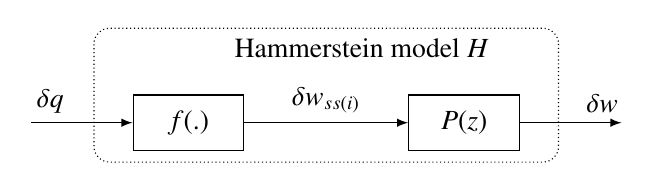
\begin{tikzpicture}[auto, node distance=2cm, >=latex] 

\node [input, name=input] {}; 
\node [block, right of=input] (nonlinear) {$f(.)$}; 
\node [block, right of=nonlinear, node distance=3.5cm] (plant) {$P(z)$};
\node [output, right of=plant] (output) {};

\draw [->] (input) -- node (deltaq) [xshift = -0.4cm]{$\delta q$} (nonlinear);
\draw [->] (nonlinear) -- node [above]{$\delta w_{ss(i)}$} (plant);
\draw [->] (plant) -- node (y) [xshift = 0.4cm] {$\delta w$} (output);

\node [coordinate, xshift = 1.2cm, yshift = 1.2cm] (upperrightcorner) at (plant) {};
\node [coordinate, xshift = -1.2cm, yshift = -0.5cm] (lowerleftcorner) at (nonlinear) {};
\draw [densely dotted, rounded corners=.2cm] (upperrightcorner) rectangle (lowerleftcorner) node [above, xshift = -2.5cm, yshift = -0.5cm, pos=0]  {Hammerstein model $H$};

\end{tikzpicture}
% }
\par\end{centering}
\begin{centering}
% \resizebox{7cm}{!}{%
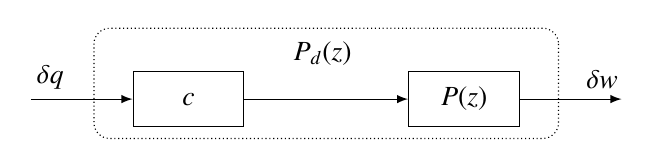
\begin{tikzpicture}[auto, node distance=2cm, >=latex] 

\node [input, name=input] {}; 
\node [block, right of=input] (nonlinear) {$c$}; 
\node [block, right of=nonlinear, node distance=3.5cm] (plant) {$P(z)$};
\node [output, right of=plant] (output) {};

\draw [->] (input) -- node (deltaq) [xshift = -0.4cm]{$\delta q$} (nonlinear);
\draw [->] (nonlinear) -- (plant);
\draw [->] (plant) -- node (y) [xshift = 0.4cm] {$\delta w$} (output);

\node [coordinate, xshift = 1.2cm, yshift = 0.9cm] (upperrightcorner) at (plant) {};
\node [coordinate, xshift = -1.2cm, yshift = -0.5cm] (lowerleftcorner) at (nonlinear) {};
\draw [densely dotted, rounded corners=.2cm] (upperrightcorner) rectangle (lowerleftcorner) node [above, xshift = -3cm, yshift = -0.6cm, pos=0]  {$P_{d}(z)$};

\end{tikzpicture}
% }
\par\end{centering}
\caption{\label{fig:Block-diagram-of-H}Block diagrams of the Hammerstein model
and the identified linear model.}
\end{figure}

\noindent 
\begin{equation}
\text{e}\rho c_{p}u_{x}=8(Bq_{0}-k)/w_{0}>0,\label{eq:e_rho_cp_ux}
\end{equation}

\noindent where $B=1/\text{[}\pi(T_{m}-T_{0})w_{0}]$ is a constant.
In (\ref{eq:analytical_sol_mpw}) and (\ref{eq:e_rho_cp_ux}), $\rho$
and $c_{p}$ are multiplied together and related to $k$. Based on
the first assumption in Section \ref{subsec:Analytical-Solutions},
we choose $k=40\,\text{W/(m}\cdot\text{k)}$ from Fig. \ref{fig:Temperature-dependent-physical-p}.
Substituting (\ref{eq:e_rho_cp_ux}) to (\ref{eq:analytical_sol_mpw})
yields

\noindent 
\begin{equation}
(Bq_{0}-k)w_{ssi}^{2}+kw_{0}w_{ssi}-Bw_{0}^{2}q=0.\label{eq:w_0}
\end{equation}

\noindent Omitting the negative root, we get

\noindent 
\begin{equation}
w_{ssi}=\frac{\sqrt{k^{2}+4(Bq_{0}-k)Bq}-k}{2(Bq_{0}-k)}w_{0}.\label{eq:w}
\end{equation}

With all parameters determined, the Hammerstein model in Fig. \ref{fig:Block-diagram-of-H}
is thus formalized around the equilibrium point by connecting (\ref{eq:w})
with $P(z)$ and letting $\delta w_{ssi}=w_{ssi}-w_{0}$ and $\delta q=q-q_{0}$.
Certainly, due to simplifications in deriving (\ref{eq:analytical_sol_mpw}),
its direct solution (\ref{eq:w}) only works at specific input conditions.
Under the input signal of $\delta q_{10}=20\text{W}\sin(2\pi ft_{s}t)$,
where $f=10\text{Hz}$ and $t_{s}$ is the sampling time, 
\begin{figure}[!ht]
\begin{centering}
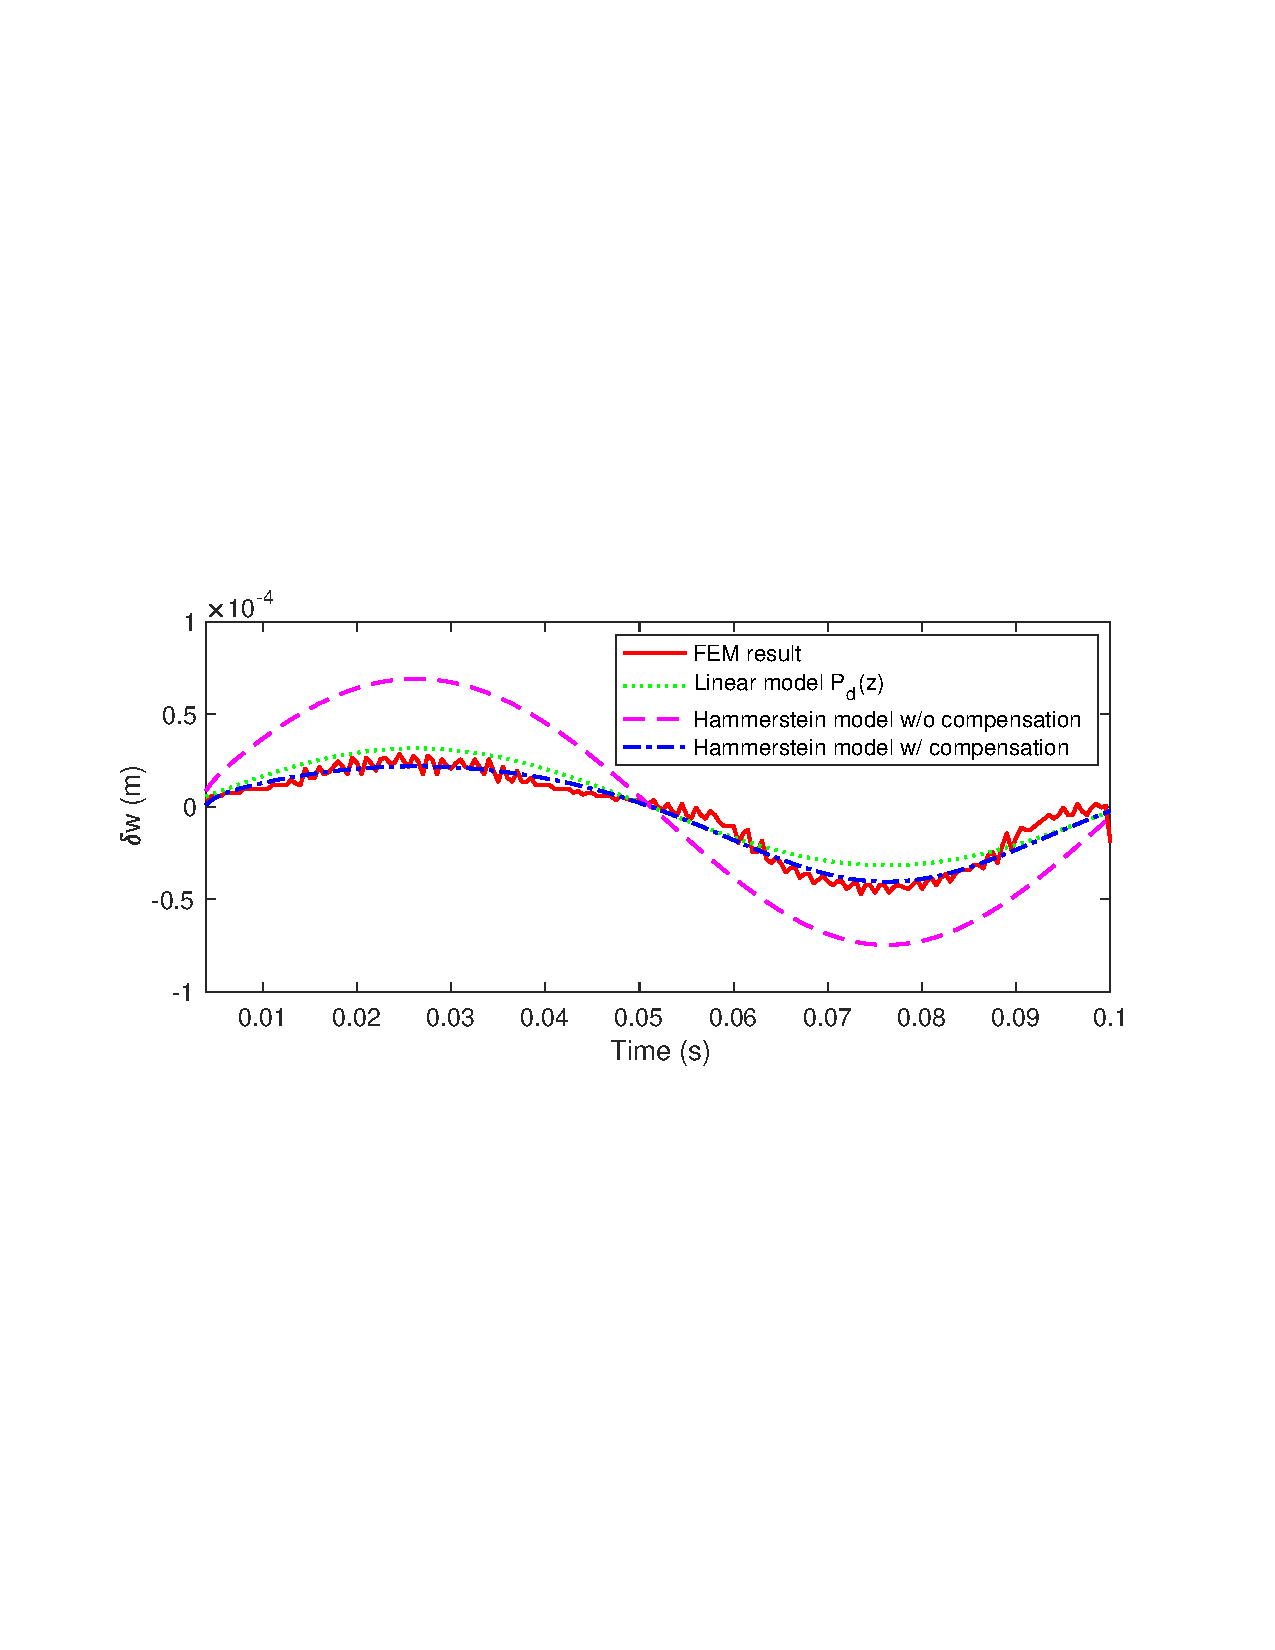
\includegraphics[clip,width=13cm]{Hammerstein/parameterID}
\par\end{centering}
\centering{}\caption{\label{fig:Parameter-identification-of}Parameter identification of
the Hammerstein model with input signal of 10 Hz.}
\end{figure}
we can tell from Fig. \ref{fig:Parameter-identification-of} that
the output of the Hammerstein model (dashed line) deviates greatly
from the FEM result (solid line).

To add more flexibility to the nonlinear block, we multiply $w_{ssi}$
in (\ref{eq:w}) with a compensation factor $\alpha(q)$:

\begin{equation}
w_{ss}=\frac{\sqrt{k^{2}+4(Bq_{0}-k)Bq}-k}{2(Bq_{0}-k)}w_{0}\alpha(q),\label{eq:w-1}
\end{equation}
where $\alpha(q)$ is a quadratic function that passes through three
points $(60\,\text{W},\,1)$ (i.e., no compensation at the equilibrium
point), $(80\,\text{W},\,\alpha_{1})$ (i.e., the maximum laser power),
and $(40\,\text{W},\,\alpha_{2})$ (i.e., the minimum laser power).
We identify the parameters $\alpha_{1}$ and $\alpha_{2}$, respectively,
as 0.8507 and 1.1973 using the Parameter Estimation tool in MATLAB.
The nonlinear least square regression is used to minimize the sum
of squared errors between the FEM data and the output of the updated
Hammerstein model with compensation (solid and dash-dotted lines in
Fig. \ref{fig:Parameter-identification-of}).

The compensated Hammerstein model is achieved by using (\ref{eq:w-1})
instead of (\ref{eq:w}) and letting $\delta w_{ss}=w_{ss}-w_{0}$.
From Fig. \ref{fig:Parameter-identification-of}, we can also tell
that this Hammerstein model (dash-dotted line) gives a better approximation
(41\% increasing) of the system dynamics (solid line) than the identified
linear model $P_{d}(z)$ (dotted line). 
\begin{figure}[!ht]
\begin{centering}
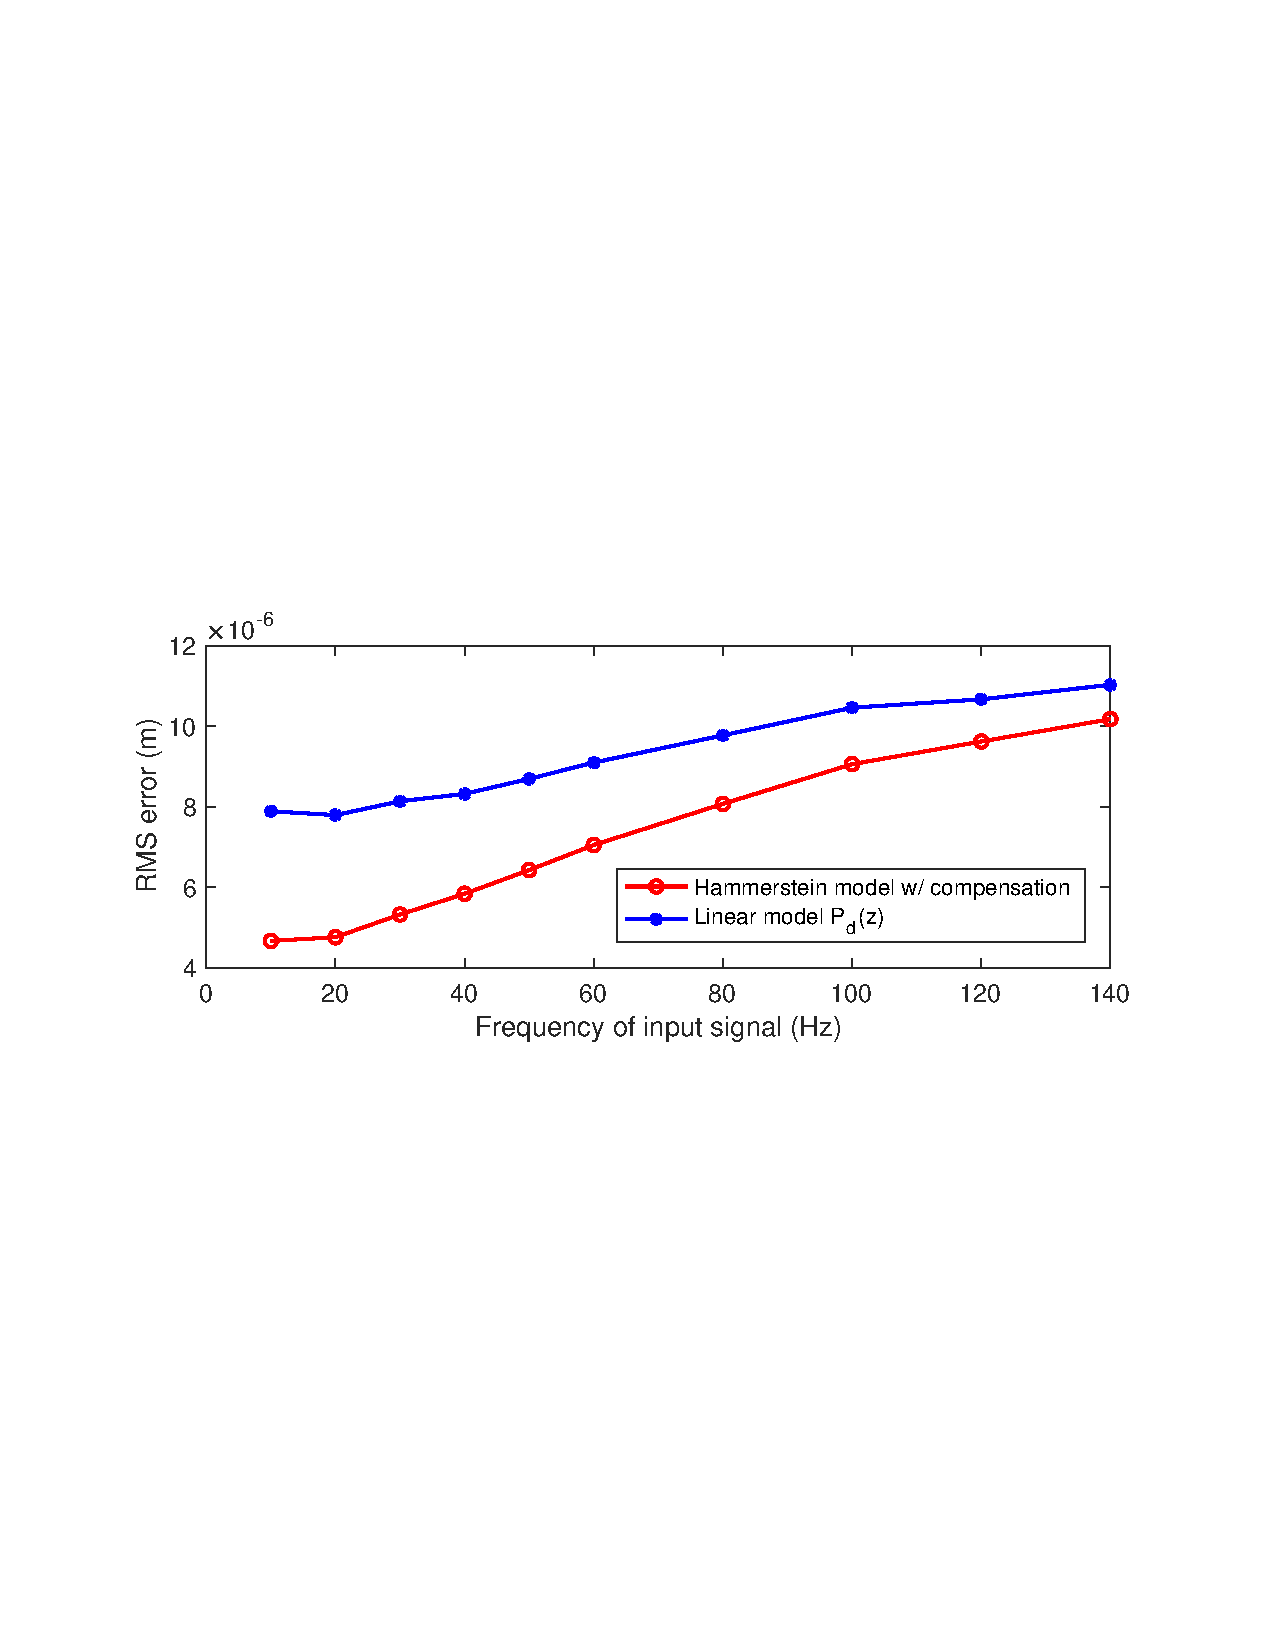
\includegraphics[clip,width=13cm]{Hammerstein/RMS_error_All_freq}
\par\end{centering}
\centering{}\caption{\label{fig:Root-mean-squared}Root mean squared (RMS) errors with
respect to different input frequencies.}
\end{figure}
More generally, as shown in Fig. \ref{fig:Root-mean-squared}, under
different input frequencies, the compensated Hammerstein model yields
smaller root mean squared errors (e.g., 4.67 \textmu m at 10 Hz)
with respect to the FEM result than the linear model (7.89 \textmu m
at 10 Hz) and achieves increasing model accuracies (41\% increasing
at 10 Hz). 
\begin{figure}
\begin{centering}
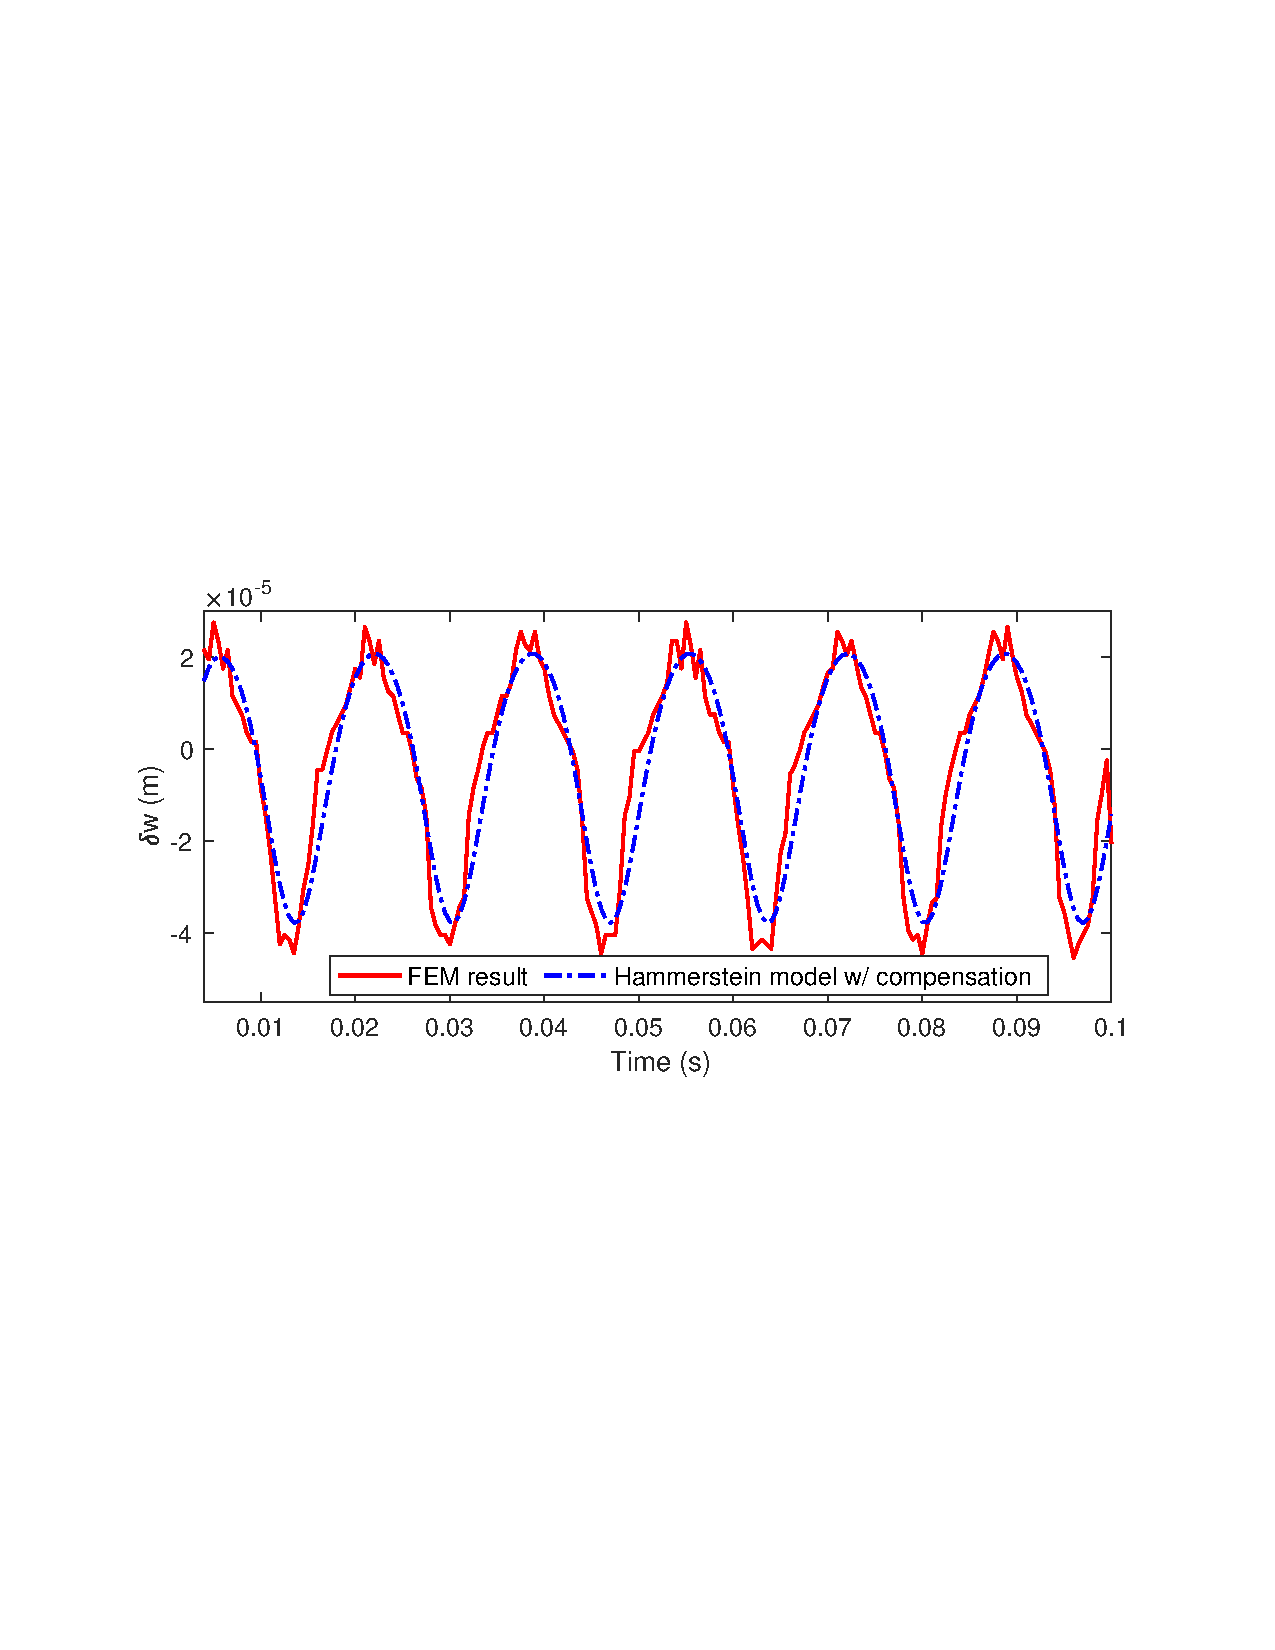
\includegraphics[clip,width=13cm]{Hammerstein/60Hz_demo}
\par\end{centering}
\centering{}\caption{\label{fig:60Hz}Melt pool width changes with input signal of 60 Hz.}
\end{figure}
Fig. \ref{fig:60Hz} illustrates the results of the compensated Hammerstein
model and the FEM under the input frequency of 60 Hz. Following the
procedures from (\ref{eq:e_rho_cp_ux}) to (\ref{eq:w-1}), we can
adaptively build the Hammerstein model for each specific equilibrium
point and structurally draw the complete model map for the entire
task space of LPBF.

We compare in Fig. \ref{fig:Steady-state-melt-pool} how $\delta w_{ss}$
changes with respect to $\delta q$ under different modeling schemes.
In the identified linear model $P_{d}(z)$, the gradient of the dash-dotted
line that links $\delta w_{ss}$ with $\delta q$ is the constant
$c$ (Fig. \ref{fig:Block-diagram-of-H}). 
\begin{figure}[!ht]
\begin{centering}
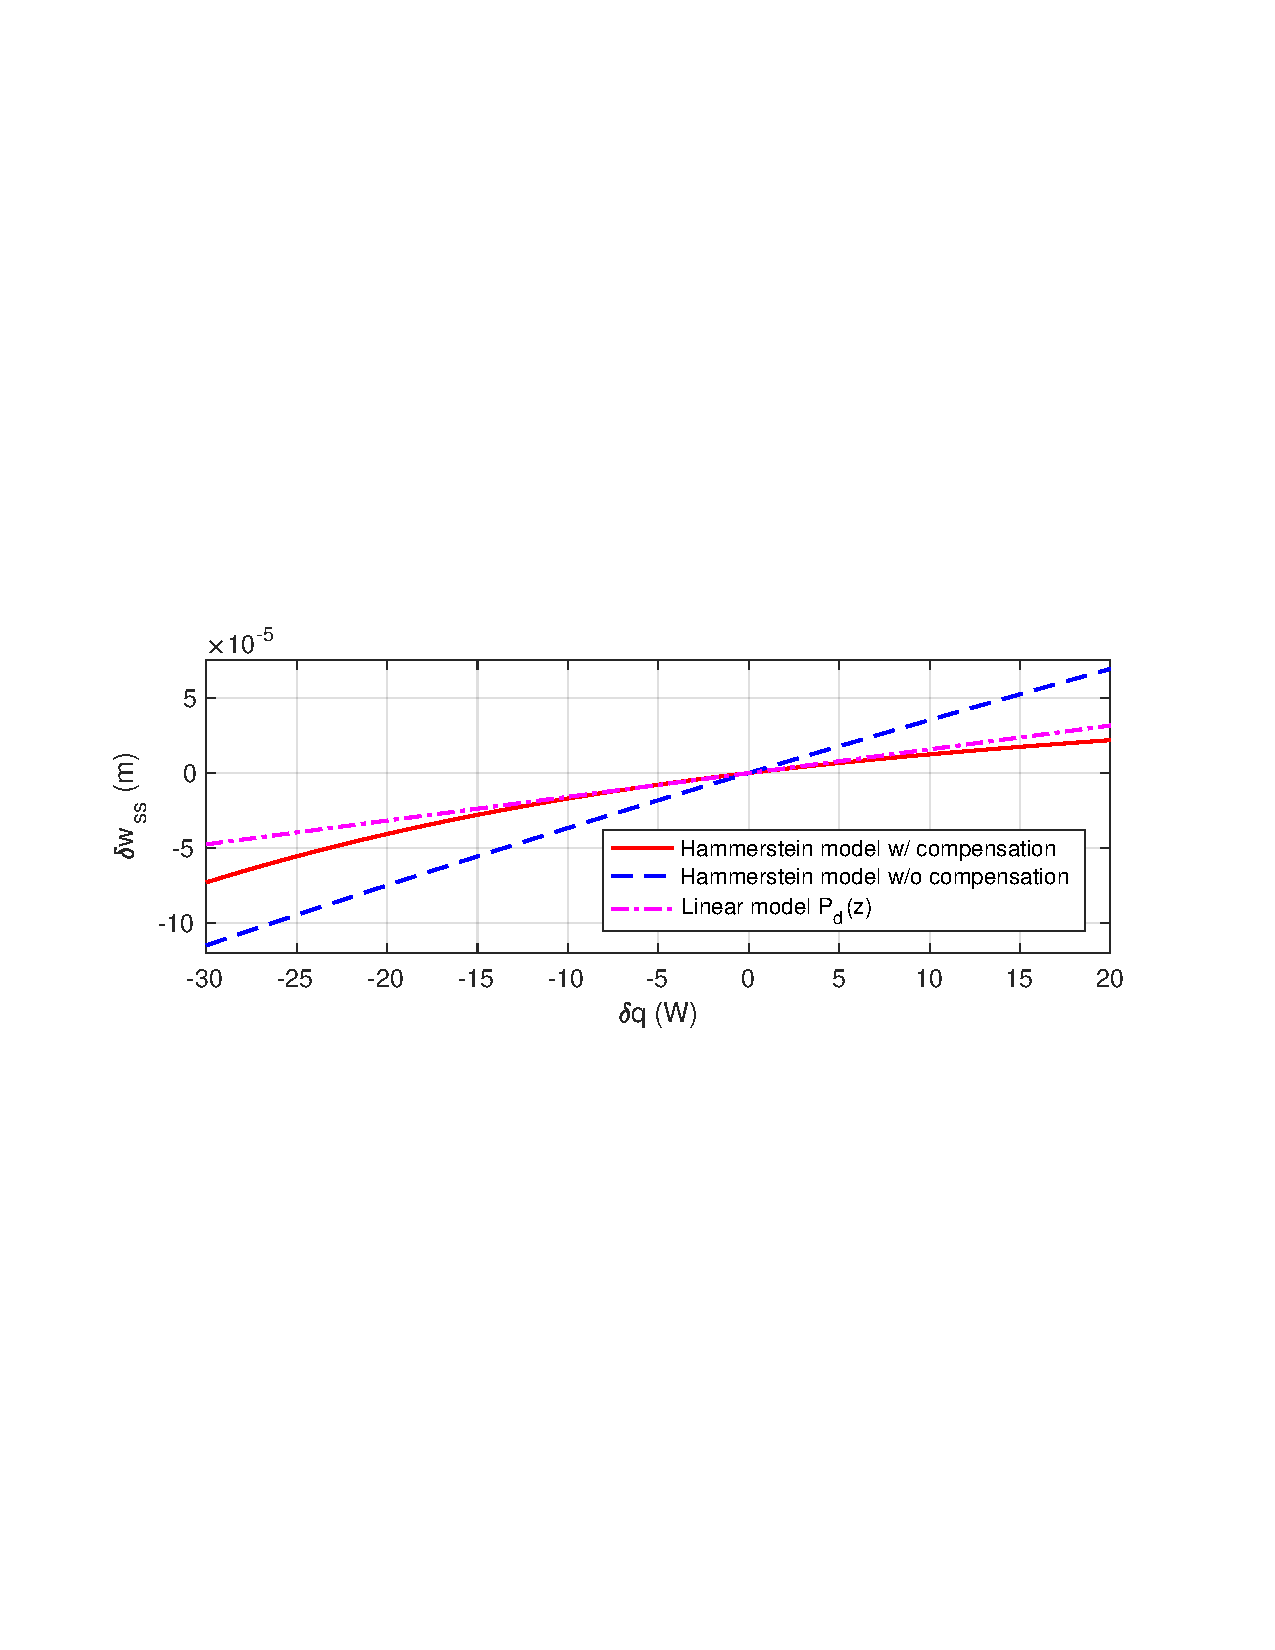
\includegraphics[clip,width=13cm]{Hammerstein/deltaWss}
\par\end{centering}
\centering{}\caption{\label{fig:Steady-state-melt-pool}Steady-state melt pool width changes
of different models.}
\end{figure}
From Fig. \ref{fig:Steady-state-melt-pool}, we can tell that $P_{d}(z)$
is only a linear representation of the nonlinear Hammerstein model
(solid line) near the equilibrium point. It is remarkable how $P_{d}(z)$
identified from the FEM data coincides tangentially with the Hammerstein
model derived from the governing equation. Next we will conduct the
stability and robustness analyses to investigate when $P_{d}(z)$
would fail in representing the Hammerstein model.

\subsection{Stability and Robustness} \label{subsec:Stability-and-Robustness}

Based on the Hammerstein model, we evaluate the robustness and stability
properties of the linear models $P_{d}(z)$ that are commonly used
in practice. Let $H=P_{d}(z)(1+\Delta)$, where $H$ is the Hammerstein
model and $\Delta$ is the bounded model uncertainty. From Fig. \ref{fig:Block-diagram-of-H},
we have $\delta w_{ss}\cdot P(z)=\delta q\cdot cP(z)(1+\Delta)$,
which gives
\begin{equation}
\left|\Delta\right|=\left|\frac{\delta w_{ss}}{c\delta q}-1\right|\label{eq:Delta}
\end{equation}

\noindent that is specified by the distance between the dash-dotted
and solid lines in Fig. \ref{fig:Steady-state-melt-pool}.

\begin{theorem} \label{thm:small-gain-theorem}
When there is (stable and bounded) model uncertainty $\Delta(z)$
such that $\hat{P}(z)=P(z)(1+\Delta(z))$, standard robust-stability
analysis\cite{chen2013selective} gives that the closed-loop system is stable if and only if both of the following
hold:
\begin{enumerate}
\item Nominal stability condition is satisfied, that is, the closed loop
is stable when $\Delta=0$.
\item Robust stability requirement is met by applying the small gain theorem
\cite{doyle2013feedback}: for any frequency $\Omega$ in Hz, $\left|\Delta\cdot T(e^{j\Omega T_{s}})\right|<1$,
that is, $\left|\Delta\right|<1/\left|T(e^{j\Omega T_{s}})\right|$,
where $T(z)$ is the complementary sensitivity function \cite{wang2018multirate}.
\end{enumerate}
\end{theorem}

Note that $\left|\Delta\right|$ in (\ref{eq:Delta}) is positively
correlated to the control signal $\delta q$, that is, more laser
power deviation from the equilibrium point yields a larger $\left|\Delta\right|$.
Under a certain frequency $\Omega$, we need to make sure the maximum
$\left|\Delta\right|$ is less than $1/\left|T(e^{j\Omega T_{s}})\right|$.
When the condition is violated, $P_{d}(z)$ will no longer be a valid
representation of the Hammerstein model.

A sufficient condition for the stability of the Hammerstein model
is the BIBO stability of the linear model $P(z)$ (Fig. \ref{fig:Block-diagram-of-H})
\cite{doyle2002identification}. In practice, the linear model is
typically a rational transfer function, whose stability can be easily
examined.

\subsection{Control Implementation}

Although the focus of this chapter is on the modeling of the complex
physics in LPBF, we have additionally presented in Fig. \ref{fig:Block-diagram-RC-H} a typical
feedback loop when applying the Hammerstein model.
\begin{figure}[!ht]
\begin{centering}
% \resizebox{8.5cm}{!}{%
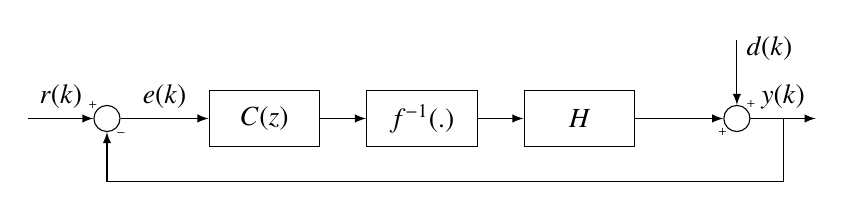
\begin{tikzpicture}[auto, node distance=2cm, >=latex] 

\node [input, name=input] {}; 
\node [sum, right of=input, node distance=1cm] (sum) {};
\node [block, right of=sum] (controller) {$C(z)$};
\node [block, right of=controller] (inv) {$f^{-1}(.)$};
\node [block, right of=inv] (plant) {$H$};
\node [sum, right of=plant](sum3) {};
\node [output, right of=sum3, node distance=1cm] (output) {};

\node [input, above of=sum3, node distance=1cm](disturbance) {};
\draw [->] (disturbance) -- node [yshift = 0.3cm]{$d(k)$} node[pos=0.99] {\tiny $+$} (sum3);

\node [coordinate, below of=controller, xshift = 0.2cm, node distance=0.8cm] (measurements) {};

\draw [->] (input) -- node {$r(k)$} node[pos=0.99] {\tiny $+$} (sum); 
\draw [->] (sum) -- node {$e(k)$} (controller);
\draw [->] (controller) -- (inv);
\draw [->] (inv) -- (plant);
\draw [->] (plant) -- node[below, pos=0.99] {\tiny $+$} (sum3);
\draw [->] (sum3) -- node (y) {$y(k)$}(output);

\draw [-] (y) |- (measurements); 
\draw [->] (measurements) -| node[right, pos=0.99] {\tiny $-$}(sum);

\end{tikzpicture}
% }
\par\end{centering}
\caption{\label{fig:Block-diagram-RC-H}Block diagram of feedback control for
a Hammerstein model.}
\end{figure}
 An $f^{-1}(\cdot)$ block is prepended with the block of
the Hammerstein model. Combining these two blocks together yields
the linear model $P(z)$. It is thereafter standard practice to design
the control algorithms for $P(z)$. To find the inverse of the nonlinear
element, we can use a high-order polynomial to approximate $f$ (solid
line in Fig. \ref{fig:Steady-state-melt-pool}). Besides, \cite{rayouf2019new}
proposes an approximate method for the cases when $f$ is not invertible.

\section{\label{sec:CONCLUSION}Summary}

In the chapter, using
the FEM data, we identify around the equilibrium point the linear
system model from the laser power to the melt pool width. In addition,
deriving from the Rosenthal equation, we reach a nonlinear closed-form
expression of the steady-state melt pool width. Concatenating the
nonlinear expression to the identified linear model, we develop the
main Hammerstein model that captures more of the convoluted thermomechanical
dynamics of LPBF. We prove that the Hammerstein mode gives a better
approximation (e.g., 41\% increasing at 10 Hz) of the FEM result than
the linear model. From there, we analyze the stability and robustness
properties of the models and present a generic control scheme for
the Hammerstein Model.

% ========== Chapter 5

\chapter{An Analytical Model of Melt Pool Width} \label{chap:Analytical-Model-MPW}

% =========================================== Part 3

\part{Multirate Feedback Control} \label{part:Multirate-Feedback-Control}

% ========== Chapter 6
 
\chapter{Loop-shaping Control} \label{chap:Loop-shaping-Control}

\section{Introduction}

A precision servo system aims at accurately positioning the controlled
object(s) to follow the desired trajectories. The controlled object
here, for instance, can be a galvo scanner for deflecting
a laser beam in LPBF \cite{wang2016spectral}, a read/write head for accessing data in
a commercial hard disk drive (HDD) \cite{atsumi2014compensating},
or a stage for carrying wafers (called wafer stage) in semiconductor
lithography \cite{oomen2014connecting}. In all examples, the required position accuracies
are quite high. Such ultra-high precision is achieved by careful
consideration of various disciplines in mechanical engineering. From
the viewpoint of system integration, the design elements are classified
to the following four categories.
\begin{itemize}
\item \emph{hardware and sensing components}: such as fluid or air bearings
for reduced friction, laser interferometers or high-precision encoders
for accurate measurements, and piezo-electronic actuators for fine
positioning;
\item \emph{operation environment}: for example, friction-isolation tables,
clean room, and thermostatic chambers;
\item \emph{task plans and arrangements}: well-designed trajectories, repetitive
tasks in a manufacturing process, etc.;
\item \emph{servo control algorithms}: adaptive control, repetitive control,
predictive control, optimal control, and so on.
\end{itemize}
A well-designed precision system needs optimized considerations in
all the above categories. Servo control, as the final step, is responsible
for compensating as much as possible the imperfections from the previous
three design processes. Such imperfections include:\emph{ }1)\emph{
hardware imperfection}, such as system resonances, delays in motor
drivers, and delays in signal acquisition; 2)\emph{ environmental
disturbance}, such as turbulent airflow, periodic disturbance from
cooling fans in HDD, and structural coupling between mirrors in the
galvo scanner; 3)\emph{ special errors due to the task nature}, such
as repeated trajectories in the wafer scanner and LPBF.

Errors from the above sources present great challenges in reaching
position accuracies at the micro/nano scale. Fortunately, part of
them\textemdash for example, imperfect motor rotation, repeated trajectories,
and fan noises\textemdash are repeatable once the hardware and the
trajectory are fixed. Other errors\textemdash such as environmental
vibrations\textemdash although may vary case by case, are at least
structured and can be compensated by carefully designed servo controllers. 

In this chapter, the loop shaping of the feedback control in precision
positioning systems is considered. In the presence of various aforementioned
error sources, the feedback loop needs to have the flexibility of
providing different closed-loop features for error reduction and guarantee
the stability under different loop modifications. To satisfy this
requirement, enhanced control at selected frequencies has been adopted
by many researchers. Based on the location of servo enhancement, enhanced
control can be categorized into three groups to deal with: (i) independent
disturbance frequencies by, for instance, peak filters \cite{li2011reset,sievers1992comparison},
adaptive feedforward cancellation \cite{Bodson1997,chen2016multirate},
disturbance observers \cite{XuChen_TCST2012,zheng2017design,chen2013selective},
and Youla-Kucera (YK) parameterization \cite{landau2005adaptive,landau2013benchmark,youla1976modern,kucera1975stability};
(ii) a fundamental frequency and its integer multiples by means of
repetitive control and its variants \cite{chen2014new,steinbuch2007design};
(iii) broadband frequencies through adaptive disturbance rejection
\cite{de2013adaptive}, adaptive noise cancellation \cite{widrow1975adaptive},
and so on. This chapter discusses recent results in enhanced control
to reach the desired servo goals. 

The main contributions of the chapter are:
\begin{itemize}
\item building flexible feedback loop-shaping schemes to compensate various
error sources in precision positioning;
\item formulating a new outer-loop inverse-based Youla-Kucera (YK) parameterization;
\item presenting a detailed case study on the galvo scanner system to validate
the proposed control algorithm.
\end{itemize}
The remainder of the chapter will unfold and discuss several feedback
control algorithms including add-on designs for precision positioning.
Section \ref{sec:FB} reviews some fundamental feedback controller
parameterizations. From there, Section \ref{sec:Instead-of-a} discusses
the proposed controller factorizations, that is, inverse-based YK
parameterization and its variant. A case study is conducted on a galvo
scanner control in Section \ref{sec:A-case-study}, and several comments
on feedforward designs are provided in Section \ref{sec:comments}.

\section{Feedback controller parameterization}

\label{sec:FB}This section briefly reviews several fundamental concepts
in feedback control and introduces YK parameterization for flexible
servo designs.

A precision positioning system is designed to have an accurate plant
dynamics $P$ which is usually linear and time-invariant. For a single-input
single-output plant controlled by linear controllers (at least at
the steady state), the position servo design can essentially be cast
as a loop shaping problem. Consider the block diagram of a standard
feedback design in Fig. \ref{fig:Block-diagram-of-fb}.
The closed-loop transfer function from the disturbance $d$ to
the plant output $y$ is defined as the sensitivity function $S\triangleq1/(1+PC)$.
The complementary sensitivity function is given by $T\triangleq1-S=PC/(1+PC)$,
that is, $T$ is the transfer function from the reference $r$ to
$y$. The sensitivity function measures the closed-loop disturbance-attenuation
property, while the complementary sensitivity function defines how
the system responds to the reference input as well as the sensor noise.
Consider a typical magnitude response of $S$ in Fig. \ref{fig:A-typical-magnitude}.
Below the bandwidth $\Omega_{c}=2\pi\omega_{c}$, the magnitude of
$S(j\Omega)$ is less than 1, which infers the attenuation of $d$
in Fig. \ref{fig:Block-diagram-of-fb}. Due to the fundamental
relationship $S+T=1$, wherever the magnitude of $S(j\Omega)$ is
small, $T(j\Omega)$ is close to unity, which means that at frequencies
where good disturbance rejection is achieved, improved reference tracking
is also obtained.

The bandwidth in Fig. \ref{fig:A-typical-magnitude} cannot be pushed
to be arbitrarily large. From the practical perspective, a mechanical
system cannot respond to arbitrarily fast control inputs due to hardware
(such as motors, gears, etc.) limitations. It is common practice to
keep the gain of the controller small at high frequencies. From the
theoretical perspective, under mild conditions,\footnote{For continuous-time systems, the waterbed effect holds if the relative
degree of the loop transfer function $L=PC$ is no less than 2. In
the discrete-time case, the waterbed effect always holds.} it is inevitable to have $|S(j\Omega^{'})|>1$ at certain frequencies
if $|S(j\Omega)|<1$ holds over some other frequency intervals, namely,
when certain disturbance components are attenuated, some others are
amplified. This is the ``waterbed'' effect which comes from Bode's
Integral Theorem, a fundamental result of linear control design. 

\begin{figure}[!ht]
\begin{centering}
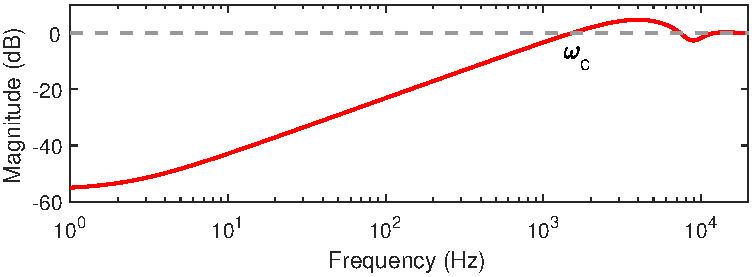
\includegraphics[width=10cm]{Loop-shaping/baseline_SISO_S_mag_3}
\par\end{centering}
\caption{\label{fig:A-typical-magnitude}Magnitude response of the sensitivity
function in Section \ref{subsec:Experimentation}}
\end{figure}

Well formulated tools such as PID, lead-lag, and $H_{\infty}$ controllers
are available to achieve a loop shape that is similar to the one in
Fig. \ref{fig:A-typical-magnitude}. We focus next on how to perform
safe and flexible add-on modifications to such a standard baseline
loop shape.

A foundational tool suitable for achieving the design goal is the
YK parameterization \cite{youla1976modern,kucera1975stability}, also
known as all-stabilizing controller parameterization. If a plant $P=N/D$
can be stabilized by a negative-feedback controller $C=X/Y$ with
($N$, $D$) and ($X$, $Y$) being coprime pairs over the set $\mathcal{S=\left\{ \text{stable, proper, and rational transfer functions}\right\} }$,
then any stabilizing feedback controller can be represented by means
of the YK parameterization as
\begin{equation}
C_{all}=\frac{X+DQ}{Y-NQ}:\ Q\in\mathcal{S},\ Y(\infty)-N(\infty)Q(\infty)\neq0.\label{eq:youla}
\end{equation}

Here a pair $\left(N,D\right)$ is called coprime over $\mathcal{S}$,
if $N,\,D\in\mathcal{S}$ and there exists $U,\,V\in\mathcal{S}$
such that $UN+VD=1$.\footnote{The inequality $Y(\infty)-N(\infty)Q(\infty)\neq0$ makes the closed
loop to be well-posed. This condition is usually easy to satisfy for
practical problems. Consider, for example, the case where $P=z^{-1}$
and $C=0.8$. We have $N=z^{-1}$, $D=1$, $X=0.8$, $Y=1$, and $Y(z=\infty)-N(z=\infty)Q(z=\infty)=1$.} 

The sensitivity function with controller (\ref{eq:youla}) in the
loop is
\begin{equation}
\tilde{S}=\frac{1}{1+PC_{all}}=\frac{1}{1+PC}\left[1-\frac{N}{Y}Q\right],\label{eq:generalYoula_S}
\end{equation}
which is affine in $Q$. Therefore, changing $Q$ can directly shape
$\tilde{S}$, which is much more convenient compared to redesigning
$C$ in the denominator of $\tilde{S}$.

For stable $P$ and $C$, one can simply choose $N=P$, $D=1$, $X=C$,
and $Y=1$ in (\ref{eq:youla}). Thus, ($N$, $D$) and ($X$, $Y$)
are valid coprime factorizations since we can pick, for example, $U=C/(1+PC)\in\mathcal{S}$
and $V=1/(1+PC)\in\mathcal{S}$ to make $UN+VD=1$. In this case,
a simplified and easier-to-use version of (\ref{eq:youla}) and (\ref{eq:generalYoula_S})
can be obtained

\begin{equation}
\tilde{C}=\frac{C+Q}{1-PQ}:\ Q\in\mathcal{S}.\label{eq:youla-simplified}
\end{equation}

\begin{equation}
\tilde{S}=\frac{1}{1+P\tilde{C}}=\frac{1-PQ}{1+PC}.\label{eq:generalYoula_S-simplified}
\end{equation}

The remaining design task about choosing $Q$ in (\ref{eq:generalYoula_S-simplified})
depends on the plant $P$ and the desired closed-loop response. For
example, candidate $Q$-filter designs can be found by using a linear
combination of some basis transfer functions (e.g., $\sum_{i=0}^{k_{Q}}\theta_{i}z^{-i}$
in discrete-time schemes), and adaptive/$H_{\infty}$ control can
be applied to find the scaling coefficients for the combination \cite{chen2013selective}.
Regardless of what tools are used, to achieve good disturbance attenuation,
$\tilde{S}$ in (\ref{eq:generalYoula_S-simplified}) is required
to be small, and hence $PQ$ should be close to 1 at the desired frequencies.
Consider a block-diagram realization in Fig. \ref{fig:A-forward-model-Youla}\footnote{In reality, $d$ is usually generated in front of the plant. When
the frequency response of the plant is known, $d$ in Fig. \ref{fig:A-forward-model-Youla}
can be mapped to $d_{0}$ in Fig. \ref{fig:Block-diagram-of-fb}
by $D_{0}(e^{j\omega})=D(e^{j\omega})P(e^{j\omega})$.}. In the inner loop marked by $\star$, $Q$ should then approximate
$P^{-1}$ to make $PQ\approx1$.
\begin{figure}[!ht]
\begin{centering}
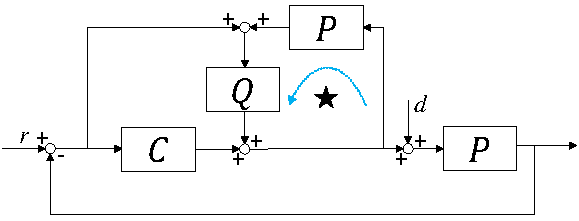
\includegraphics[width=9cm]{Loop-shaping/block diagram-2}
\par\end{centering}
\caption{\label{fig:A-forward-model-Youla}A forward-model YK parameterization}
\end{figure}

\section{Proposed controller factorization} \label{sec:Proposed0-controller-factorization}

\label{sec:Instead-of-a}Instead of a direct inversion of $P$ by
$Q$, this section discusses an alternative scheme that brings additional
simplifications to (\ref{eq:generalYoula_S-simplified}). Although
a general analysis can be made, we focus on precision servo systems
and assume that the baseline controller $C$ is stable. 

Consider designing inverse-based YK parameterization in two steps:
first to perform a stable model inversion $P^{-1}$ and second to
use $Q$ for controlling the amount of loop shaping and disturbance
rejection. Of course, a perfect inversion of the plant dynamics is
practically impossible, and a nominal version $\hat{P}^{-1}$ has
to be adopted. In addition, during discrete-time implementation, the
sampled-data transfer function $\hat{P}^{-1}(z)$ is possibly not
causal/realizable since a practical plant $P$ usually has delays
(suppose $m$ steps of delays) that become $z^{m}$ when inverted, where $z$ is the complex indeterminate in $z$-transform.
For realizability, consider using instead $z^{-m}\hat{P}^{-1}(z)$.
For the moment, $\hat{P}^{-1}(z)$ is assumed to be stable. This is
not difficult to achieve for precision positioning systems. Chapter \ref{chap:Model-Inversion} will discuss more about this model inversion topic. A block
diagram of the alternative scheme is shown in Fig. \ref{fig:Block-diagram-RC}.
Compared to Fig. \ref{fig:A-forward-model-Youla}, this discrete-time
scheme is closer to actual implementation, and modifications have
been made to reduce the dependence of the plant information in the
($\star$) loop in Fig. \ref{fig:A-forward-model-Youla}. 
\begin{figure}[!ht]
\begin{centering}
% \resizebox{8.4cm}{!}{%
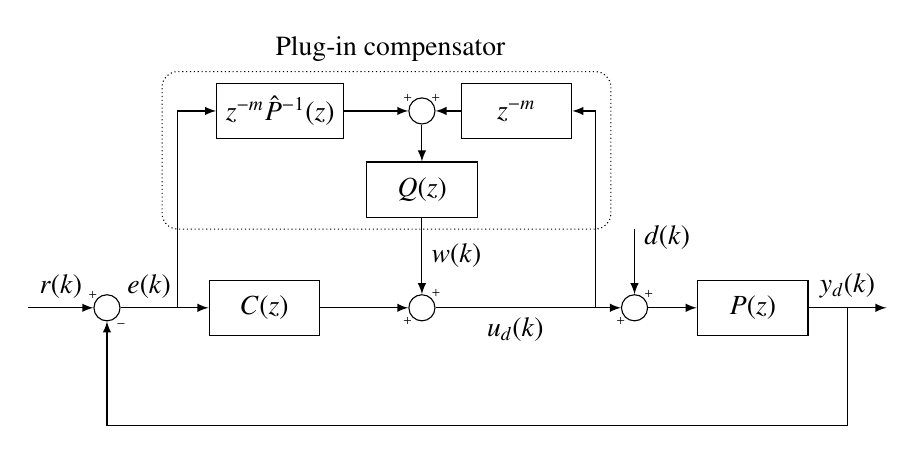
\begin{tikzpicture}[auto, node distance=2cm, >=latex] 

\node [input, name=input] {}; 
\node [sum, right of=input, node distance=1cm] (sum) {};
\node [coordinate, right of=sum, xshift = 0.4cm, node distance=0.5cm] (sumC) {};

\node [block, right of=sum] (controller) {$C(z)$}; 
\node [sum, right of=controller] (sum2) {};
\node [coordinate, right of=sum2, xshift = 0.2cm] (sum2sum3) {};

\node [sum, right of=sum2sum3, node distance=0.5cm] (sum3) {};
\node [block, right of=sum3, node distance=1.5cm] (plant) {$P(z)$};
\node [output, right of=plant, node distance=1.7cm] (output) {};
\node [block, above of=sum2, node distance=1.5cm] (Q) {$Q(z)$};
\node [sum, above of=Q, node distance=1cm] (sum4) {};
\node [block, xshift = 0.2cm, left of=sum4] (Phat) {$z^{-m}\hat{P}^{-1}(z)$};
\node [block, right of=sum4, node distance=1.2cm] (Zm) {$z^{-m}$};

\node [coordinate, below of=controller, xshift = 0.2cm, node distance=1.5cm] (measurements) {};

\node [input, above of=sum3, node distance=1cm](disturbance) {};
\draw [->] (disturbance) -- node [yshift = 0.3cm]{$d(k)$} node[pos=0.99] {\tiny $+$} (sum3);

\draw [->] (input) -- node {$r(k)$} node[pos=0.99] {\tiny $+$} (sum); 
\draw (sum) -- node {$e(k)$} (sumC); 
\draw [->] (sumC) -- (controller);
\draw [->] (controller) -- node[below, pos=0.99] {\tiny $+$} (sum2);
\draw (sum2) -- node [below] {$u_{d}(k)$} (sum2sum3);
\draw [->] (sum2sum3) -- node[below, pos=0.99] {\tiny $+$} (sum3);
\draw [->] (sum3) -- (plant);
\draw [->] (plant) -- node (y) {$y_{d}(k)$}(output); 
\draw [-] (y) |- (measurements); 
\draw [->] (measurements) -| node[right, pos=0.99] {\tiny $-$}(sum);

\draw [->] (sumC) |- (Phat);
\draw [->] (Phat) -- node[pos=0.99] {\tiny $+$} (sum4);
\draw [->] (sum4) -- (Q);
\draw [->] (Q) -- node {$w(k)$} node[pos=0.99] {\tiny $+$} (sum2);
\draw [->] (Zm) -- node[above, pos=0.99] {\tiny $+$} (sum4);
\draw [->] (sum2sum3) |- (Zm);

\node [coordinate, xshift = 1.2cm, yshift = 0.5cm] (upperrightcorner) at (Zm) {};
\node [coordinate, xshift = -0.2cm, yshift = 1cm] (lowerleftcorner) at (sumC) {};

\draw [densely dotted, rounded corners=.2cm] (upperrightcorner) rectangle (lowerleftcorner) node [above, xshift = -2.8cm, pos=0]  {Plug-in compensator};

\end{tikzpicture}
% }
\par\end{centering}
\caption{\label{fig:Block-diagram-RC}Block diagram of a plug-in RC design.}
\end{figure}

The transfer function of the overall feedback controller from $e(k)$ to $y_d(k)$ in Fig. \ref{fig:Block-diagram-RC}
is
\begin{equation}
C_{all}(z)=\frac{C(z)+z^{-m}\hat{P}^{-1}(z)Q(z)}{1-z^{-m}Q(z)},\label{eq:proposedYoula}
\end{equation}
where high-gain control (increased control effort) is directly provided
by $1/(1-z^{-m}Q(z))$ instead of $1/(1-PQ)$ in (\ref{eq:youla-simplified}).
This reduced dependence on $P$ is also reflected in the frequency
sensitivity function $\tilde{S}(e^{j\omega})=\left.\tilde{S}(z)\right|_{z=e^{j\omega}}$.
If $\hat{P}(e^{j\omega})=P(e^{j\omega})$, (\ref{eq:proposedYoula})
gives
\begin{align}
\tilde{S}(e^{j\omega}) & =\frac{1}{1+P(e^{j\omega})C_{all}(e^{j\omega})}=\frac{1-e^{-mj\omega}Q(e^{j\omega})}{1+P(e^{j\omega})C(e^{j\omega})}\nonumber \\
 & =\left.S_{0}(z)(1-z^{-m}Q(z))\right|_{z=e^{j\omega}}.\label{eq:proposedYoula_S_S0}
\end{align}

In some practices, when the plant and built-in controller (e.g.,
designed by manufacturers in the factory) are lumped together, only
signals $v$ and $y$ in Fig. \ref{fig:A-discrete-time-inverse-based-1-1}
are accessible, and separating the plant model $P_{e}$ is infeasible.
In this circumstance, an outer loop can be designed by adding one
positive feedback loop and, at the same time, one negative feedback
loop outside the original loop shaping, as shown in Fig. \ref{fig:A-discrete-time-inverse-based-1-1}.
With $C=1$, the servo performance of the original feedback loop keeps
unchanged. Take $L(z)\triangleq P_{e}C_{e}$ as the new plant. This
augmented plant model $L(z)$ can be computed from $T_{e}(z)$, the
transfer function from $v$ to $y$, by $L(z)=T_{e}(z)/(1-T_{e}(z))$.
Then the controller $C(=1)$ can be extended to obtain the desired
closed-loop response. In Fig. \ref{fig:A-outer-loop-inverse-based},
the inverse-based YK parameterization is added on $C$. With $C(e^{j\omega})=1$
as well as $P(e^{j\omega})$ replaced by $L(e^{j\omega})$ in (\ref{eq:proposedYoula})
and (\ref{eq:proposedYoula_S_S0}), the outer-loop inverse-based YK
parameterization gives

\begin{equation}
C_{all}(z)=\frac{1+z^{-m}\hat{L}^{-1}(z)Q(z)}{1-z^{-m}Q(z)}.\label{eq:outer_loop_Youla}
\end{equation}

\begin{align}
\tilde{S}(e^{j\omega}) & =\left.\frac{1}{1+L(e^{j\omega})}(1-z^{-m}Q(z))\right|_{z=e^{j\omega}}.\label{eq:L_S_frequency response}
\end{align}

Nominal stability of the closed-loop system can be guaranteed given
proper coprime factorizations. Summarizing the requirements in each
of the four introduced YK schemes yields Table \ref{tab:Nominal-stability-conditions}.
\begin{figure}[!ht]
\begin{centering}
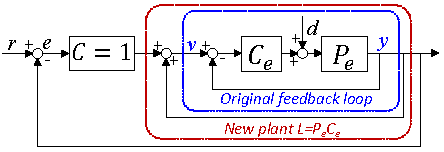
\includegraphics[width=9cm]{Loop-shaping/block diagram-BL}
\par\end{centering}
\caption{\label{fig:A-discrete-time-inverse-based-1-1}An outer-loop block
diagram}
\end{figure}
\begin{figure}[!ht]
\begin{centering}
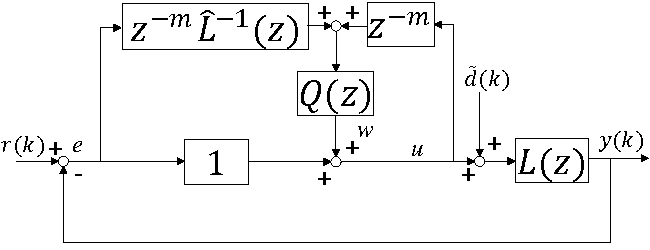
\includegraphics[width=9cm]{Loop-shaping/L-YK parameterization}
\par\end{centering}
\caption{\label{fig:A-outer-loop-inverse-based}An outer-loop inverse-based
YK parameterization}
\end{figure}
\begin{table}[!ht]
\caption{\label{tab:Nominal-stability-conditions}Nominal stability conditions
for the four add-on designs.}
\begin{centering}
% \footnotesize

\setlength\tabcolsep{1.5pt}

\begin{tabular}{cccc} 

\toprule

\makecell{YK \\ parameterization} & \makecell{Simplified YK \\ parameterization} & \makecell{inverse-based YK \\ parameterization} & \makecell{Outer-loop YK \\ parameterization}\\

\midrule

$Q\in\mathcal{S}$ & $P$, $C$, $Q\in\mathcal{S}$ & $\hat{P}^{-1}$, $C$, $Q\in\mathcal{S}$ & $\hat{L}^{-1}$, $Q\in\mathcal{S}$\\

\bottomrule
\end{tabular}
\par\end{centering}
\end{table}

\noindent \begin{remark}The robust stability requirement in Theorem \ref{thm:small-gain-theorem} in Section \ref{subsec:Stability-and-Robustness} is
not difficult to satisfy. Take the inverse-based YK parameterization
in (\ref{eq:proposedYoula_S_S0}) as an example, where $\tilde{T}(e^{j\omega})$
is given by

\begin{align}
\tilde{T}(e^{j\omega}) & =\frac{\hat{P}(e^{j\omega})C(e^{j\omega})+e^{-mj\omega}Q(e^{j\omega})}{1+\hat{P}(e^{j\omega})C(e^{j\omega})}.\label{eq:L_S_frequency response-1}
\end{align}

If $Q(e^{j\omega})=0$, $\tilde{T}(e^{j\omega})$ reduces to the original
complementary sensitivity function $T_{0}(e^{j\omega})$ without the
add-on design. We thus have $\left|\Delta(e^{j\omega})T_{0}(e^{j\omega})\right|<1$,
which is the robust stability condition of the baseline feedback loop.
If $e^{-mj\omega}Q(e^{j\omega})=1$, $\tilde{T}(e^{j\omega})=1$.
At these frequencies, $\left|\Delta(e^{j\omega})\right|<1$ is required,
that is, the mismatch between $P(e^{j\omega})$ and $\hat{P}(e^{j\omega})$
has to be less than 100\%.\end{remark}

In (\ref{eq:proposedYoula_S_S0}) and (\ref{eq:L_S_frequency response}),
the add-on design narrows down to the design of $1-z^{-m}Q(z)$, which
is much simpler than $1-PQ$ in (\ref{eq:generalYoula_S-simplified})
and $1-NQ/Y$ in (\ref{eq:generalYoula_S}). Several general design
guides for $Q(z)$ can now be made.

\subsection{Low-frequency Servo Enhancement}

An intuitive choice for $Q(z)$ is a low-pass filter. In this case,
if the delay of the plant is not very large, then the frequency transfer
function $1-e^{-j\omega m}Q(e^{j\omega})$ would be small when $Q(e^{j\omega})$
is approximately one at low frequencies and be close to unity when
$|Q(e^{j\omega})|\ll1$ at high frequencies. A direct result is that
any bias disturbance can be rejected. This is because under the low-pass
assumption, $1-e^{-jm\times0}Q(e^{j\times0})=1-Q(e^{j\times0})=0$
at $\omega=0$. Therefore, an integral action is built into the closed-loop
controller.

\subsection{Narrow-band Disturbance Rejection}

\label{subsec:NarrowBand_loopShaping}Vibrations are frequency-dependent
signals by nature. Since the closed-loop bandwidth cannot be arbitrarily
increased, vibrations at frequencies above the servo bandwidth are
fundamentally more difficult to handle. Actually, such band-limited
disturbances, if strong enough, significantly limit the servo performance.
To compensate for such vibrations, some special feedback adjustments
are needed. Meantime, we commonly want to keep as much as possible
the original loop shape because it is often achieved by means of careful
baseline design. A candidate add-on design is to use the proposed
inverse-based YK parameterization and design a notch shape for $1-z^{-m}Q(z)$
such as the one shown in the bottom plot of Fig. \ref{fig:A-loop-shaping}.
To demonstrate the flexibility, five notches are introduced in the
magnitude of $1-z^{-m}Q(z)$. The first three notches are very close
to each other, and the other two are separated at higher frequencies.
When $1-e^{-mj\omega}Q(e^{j\omega})$ is close to unity, $\tilde{S}(e^{j\omega})=\left.S_{0}(z)(1-z^{-m}Q(z))\right|_{z=e^{j\omega}}$
is close to $S_{0}(e^{j\omega})$, and hence the original loop shape
is maintained. At frequencies where $1-z^{-m}Q(z)$ has very small
gains in Fig. \ref{fig:A-loop-shaping}, the overall controller (\ref{eq:proposedYoula})
then has high gain, $\tilde{S}(e^{j\omega})$ is very small, and hence
vibrations can be attenuated.

An example about disturbance attenuation in a HDD benchmark problem
\cite{sun2016enhanced} is presented in Fig. \ref{fig:Frequency-spectra-of-1}.
This benchmark has been used in a number of publications on information
storage systems. The compensation scheme is implemented for rejecting
two strong vibrations at around 1100 Hz and 1500 Hz. Both vibrations
occur at frequencies above the baseline servo bandwidth (1060 Hz)
and cannot be attenuated in the standard feedback setting. After compensation,
the two originally sharp spectral peaks are actually visually not
detectable due to the deep notch shape of $1-z^{-m}Q(z)$ in Fig.
\ref{fig:A-loop-shaping}.
\begin{figure}[!ht]
\begin{centering}
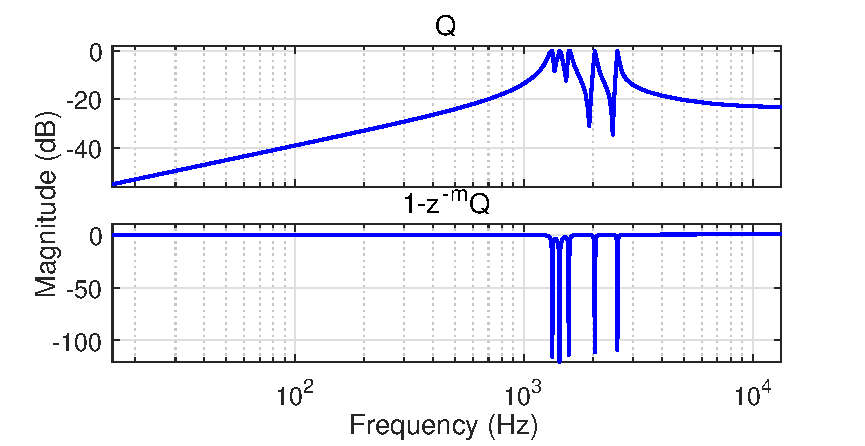
\includegraphics[width=13cm]{Loop-shaping/Q1minusQ}
\par\end{centering}
\caption{\label{fig:A-loop-shaping}A Q-design example for narrow-band disturbance
rejection}
\end{figure}
\begin{figure}[!ht]
\begin{centering}
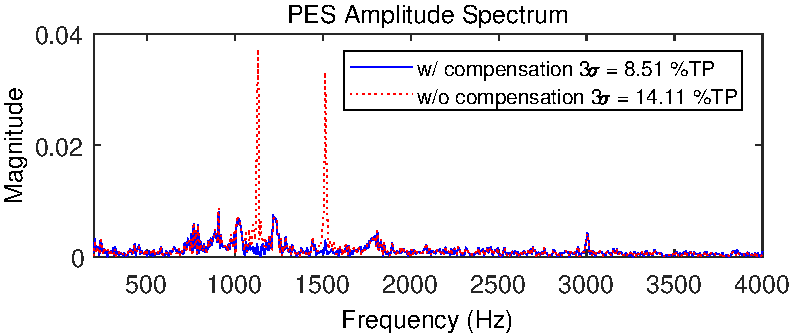
\includegraphics[width=13cm]{Loop-shaping/freqDomain_specPES_compare_iter8_linear}
\par\end{centering}
\caption{\label{fig:Frequency-spectra-of-1}Frequency spectra of the position
error signals in a simulated HDD benchmark: $1$ TP (Track Pitch)
= 254nm in this example.}
\end{figure}

Take the example of $m=1$. The key concept of Q design is to have
a notch shape of $1-z^{-1}Q(z)$ at certain disturbance frequency
$\omega_{0}=2\pi f_{0}T_{s}$, where $T_{s}$ is the sampling time
and $f_{0}$ is in Hz. Designing $1-z^{-1}Q(z)=\frac{1-2\cos\omega_{0}z^{-1}+z^{-2}}{1-2\alpha\cos\omega_{0}z^{-1}+\alpha^{2}z^{-2}}$
and solving for $Q(z)$ gives
\begin{equation}
Q(z)=\frac{a(\alpha-1)+(\alpha^{2}-1)z^{-1}}{1+a\alpha z^{-1}+\alpha^{2}z^{-2}},\ a=-2\cos(\omega_{0}).\label{eq:singleQ}
\end{equation}

Extending (\ref{eq:singleQ}), if multiple notches are desired, with
$1-z^{-1}Q(z)=A(z^{-1})/A(\alpha z^{-1})$, $A(\alpha z^{-1})=\prod_{i=1}^{n}(1-2\cos(\Omega_{i}T_{s})\alpha z^{-1}+\alpha^{2}z^{-2})$,
and $A(z^{-1})=\left.A(\alpha z^{-1})\right|_{\alpha=1}$, letting
$Q(z)=B_{Q}(z^{-1})/A_{Q}(z^{-1})$ gives the general solution
\begin{align}
A_{Q}(z^{-1}) & =1+\sum_{i=1}^{n-1}a_{i}(\alpha^{i}z^{-i}+\alpha^{2n-i}z^{-2n+i})+a_{n}\alpha^{n}z^{-n}+\alpha^{2n}z^{-2n}.\nonumber \\
B_{Q}(z^{-1}) & =\sum_{i=1}^{2n}(\alpha^{i}-1)a_{i}z^{-i+1}.\ a_{i}=a_{2n-i}.\label{eq:mQ}
\end{align}


Here $\alpha(<1)$ controls the width of the attenuation regions and
can be taken very close to 1 for narrow-band disturbance rejection.
The coefficients $a_{i}$'s in (\ref{eq:singleQ}) and (\ref{eq:mQ})
determine the notch frequencies of $Q(z)$. In (\ref{eq:mQ}), $a_{i}$
and the desired notch frequency $\Omega_{i}$ in rad/s are connected
by the mapping $A_{Q}(z^{-1})=A(\alpha z^{-1})$. 

When $m>1$, several additional steps are needed since $1-z^{-m}Q(z)=A(z^{-1})/A(\alpha z^{-1})$
would not have a realizable solution. An approach that uses Diophantine
identity to address this issue is provided in the reference \cite{XuChen_TCST2012}.
Specifically, when $m=2$, the expression of $Q(z)$ is
\begin{equation}
Q(z)=\frac{\left[\alpha^{2}-1-a^{2}(\alpha-1)\right]-a(\alpha-1)z^{-1}}{1+a\alpha z^{-1}+\alpha^{2}z^{-2}},\label{eq:singleQ_m_2}
\end{equation}
where $\alpha$ and $a$ have the same meanings as those in (\ref{eq:singleQ}).

\subsection{Repetitive Control} \label{subsec:repetitive-control}

An example application of repetitive control is for addressing the
problem involved in wafer-scanning process, one key step for circuit
fabrication in the semiconductor industry. To print the circuit, the
wafer is exposed to patterned ultraviolet lights that come through
a mask carried by a reticle stage. The wafer stage and the reticle
stage move the wafer and the mask in a synchronized manner. Due to
the limited size of the lens, only a small part of the wafer is exposed
at each scan, and the wafer is moved from one field to another between
the scans. The scanning process is repeated until all required areas
on the wafer have been exposed under the light. An intuition about
repetitive control is that if the same type of disturbance occurs
after a fixed period of time, that is, $d(k)=d(k-N_{d})$ where $N_{d}$
is the period of the disturbance, then at the next occurrence of $d(k)$,
we can learn and reduce the resulting error, no matter how it behaves
within one period of time. From the spectral perspective, the magnitude
response of $1-z^{-m}Q(z)$ in Fig. \ref{fig:Q_wideband}
provides a typical loop shape for repetitive control that $|1-e^{-jm\omega}Q(e^{j\omega})|$
gives low gains to $|\tilde{S}(e^{j\omega})|$ at the fundamental
frequency and its integer multiples. Meanwhile, at other frequencies
$|1-e^{-jm\omega}Q(e^{j\omega})|$ is approximately unity yielding
no change to $|\tilde{S}(e^{j\omega})|$. More details will be provided in Chapter \ref{chap:Fractional-RC}.

\subsection{General Band-limited Vibration Compensation}

The loop shaping in Section \ref{subsec:NarrowBand_loopShaping} is
for narrow-band disturbance rejection. When excitation sources are
rich in frequency, a wider attenuation bandwidth of $1-z^{-m}Q(z)$
is needed and can be achieved by changing the design parameter $\alpha$
in (\ref{eq:singleQ}) and (\ref{eq:mQ}), which is related to the
width of the $-3\,\text{dB}$ passband for $1-z^{-m}Q(z)$ by $BW\approx(1-\alpha^{2})/[(\alpha^{2}+1)(\pi T_{s})]$
(Hz) \cite{chen2013inverse}. As the disturbance attenuation is pushed
further, the trade-off amplification due to the waterbed effect also
increases. Additional design considerations are therefore necessary
for a safe implementation. Fig. \ref{fig:The-control-of} shows the
loop-shaping result on a HDD benchmark example. No large sensitivity
amplifications are observed due to: (i) a gain scheduling in the $Q$-filter
with $Q_{\text{implement}}=k_{Q}Q(z)$ ($k_{Q}\leq1$); (ii) the use
of a damped notch filter $F_{nf}(z)=A(\beta z^{-1})/A(\alpha z^{-1})$
($\alpha<\beta<1$) in the design of $Q(z)$. Auxiliary zeros and
convex optimization can be applied for specific magnitude constraints
on $Q(z)$ \cite{chen2014optimal}.
\begin{figure}[!ht]
\begin{centering}
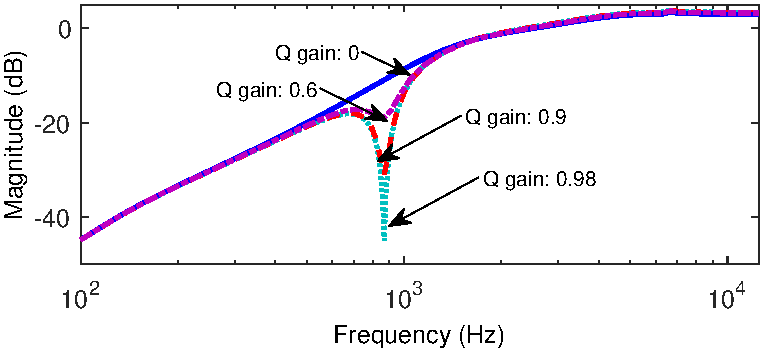
\includegraphics[width=13cm]{Loop-shaping/bandlimited_bode_S_Qgian_scheduling}
\par\end{centering}
\caption{\label{fig:The-control-of}The control of attenuation efforts by means
of gain scheduling on $Q$}
\end{figure}

\section{A Case Study on a Galvo Scanner System} \label{sec:A-Case-Study-on-a-Galvo-Scanner-System}

\label{sec:A-case-study} In this section, we provide the design and
analysis steps for implementing the (outer-loop) inverse-based YK
parameterization on a galvo scanner platform to verify the effectiveness
of the proposed servo design. In LPBF, laser beams are controlled to melt the powder materials
following pre-designed trajectories. Rather than moving the laser
source, LPBF efficiently applies a galvo scanner platform to reflect
the laser beams. Besides LPBF, the galvo scanner platform is also widely
used in other laser-related applications, such as laser scanning, laser
engraving, and laser welding.
\begin{figure}[!ht]
\begin{centering}
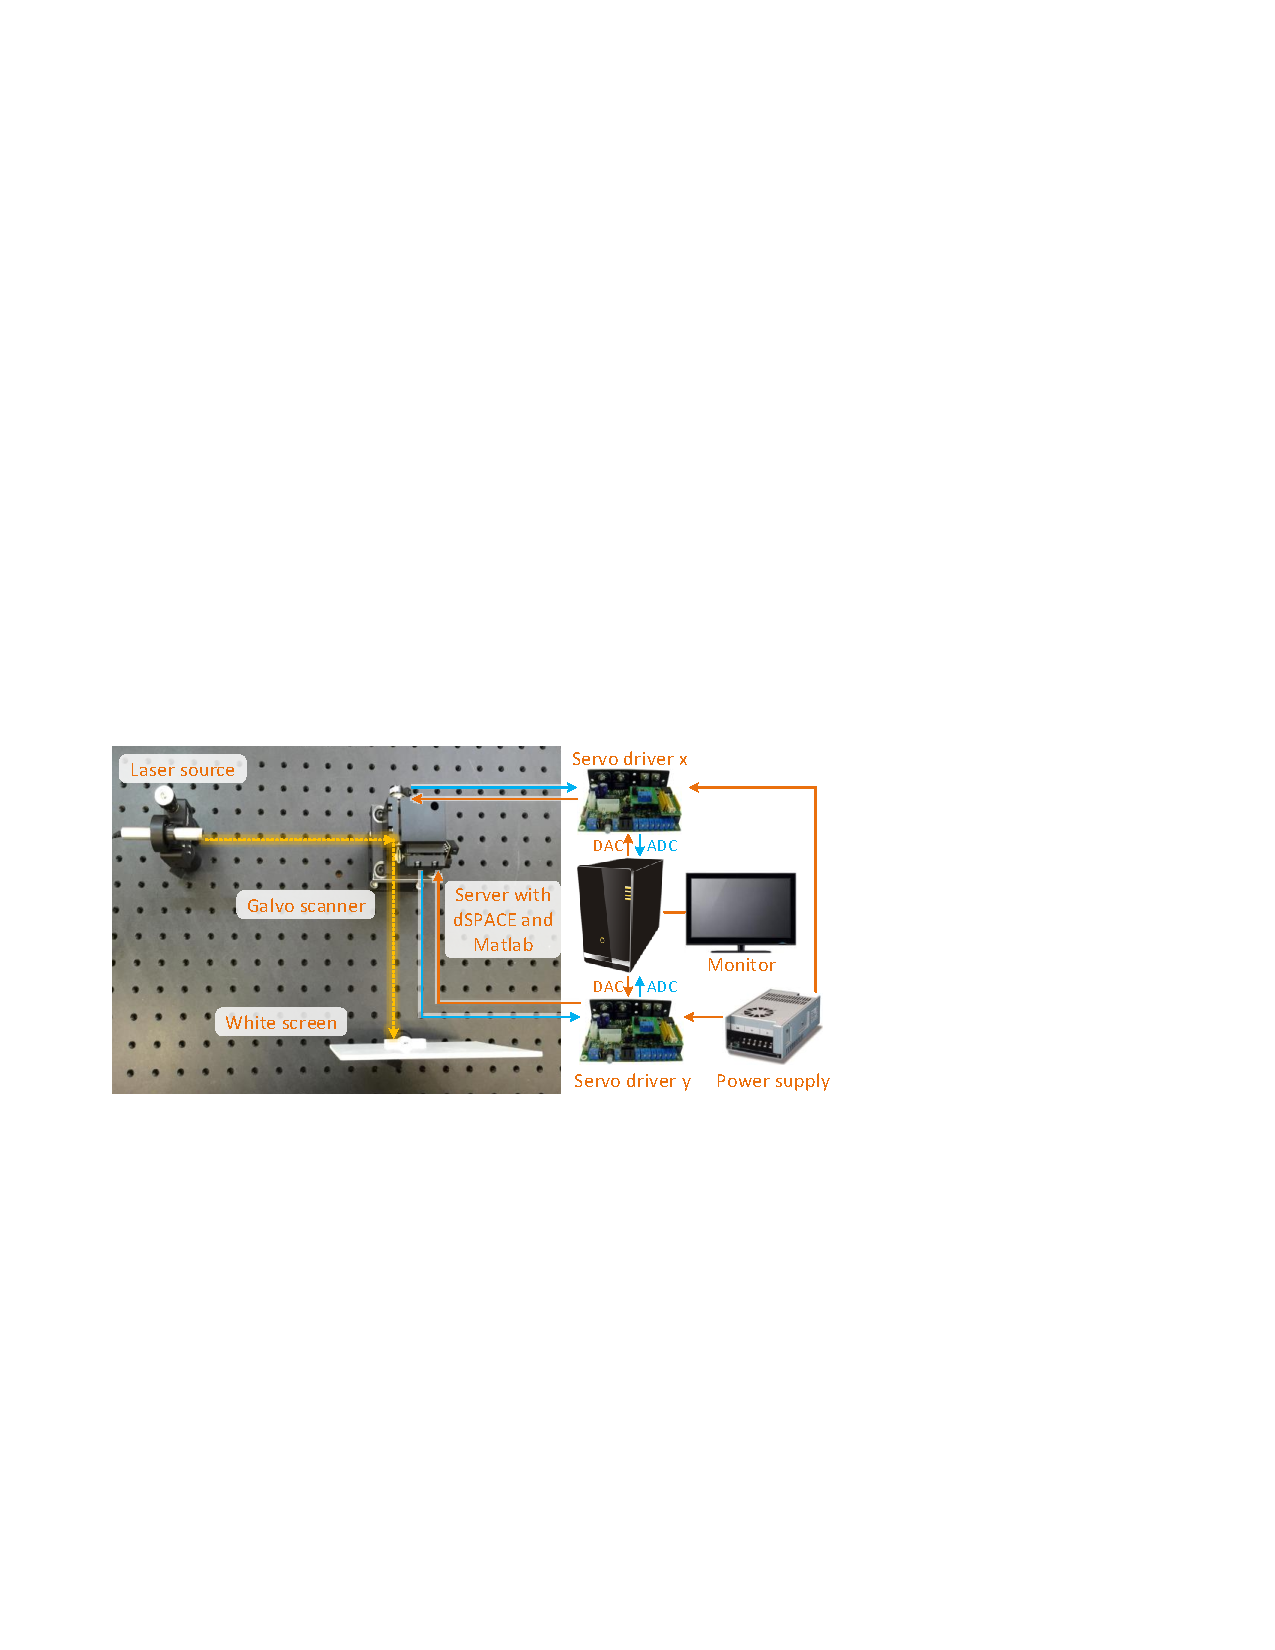
\includegraphics[width=13cm]{Fractional-order-RC/system setup}
\par\end{centering}
\caption{\label{fig:Schematic-of-hardware-LS}Schematic of the galvo scanner platform}
\end{figure}

A typical galvo scanner platform is composed of two sets of mirrors,
galvanometers, and control systems, as shown in Fig. \ref{fig:Schematic-of-hardware-LS}. The galvanometer consists of motors to rotate the mirrors and encoders
to feedback the mirror position information. A dSPACE DS1104 board connects control system designs in MATLAB with the servo drivers. The mirror assembly is
attached to the end of the motors in a coaxial manner and deflects
the laser beam over the angular range of the motor shaft, as shown
in Fig. \ref{fig:Schematic-diagram-of-G}. $O_{1}$ and $O_{2}$ indicate
the centers of the two mirrors, and the corresponding rotation angles
are denoted as $\gamma$ and $\delta$, respectively. $L_{1}$ is
the distance between the two mirror centers, and $L_{2}$ represents
the distance between mirror $O_{2}$ and the image field $O$.
\begin{figure}[!ht]
\begin{centering}
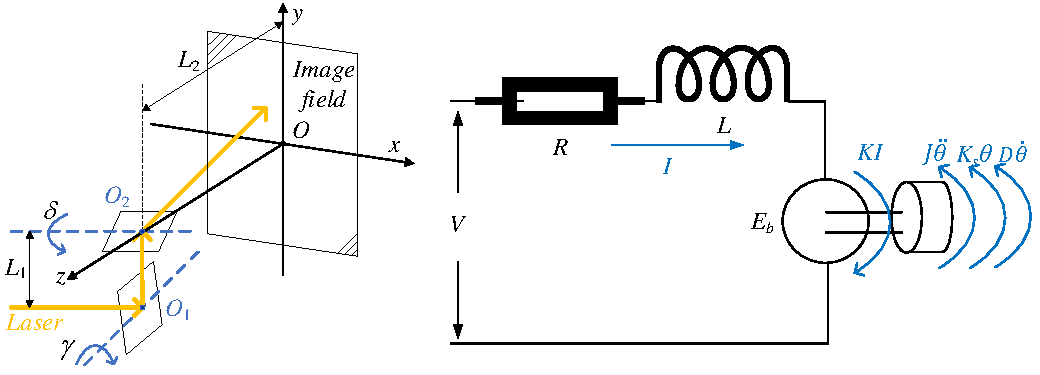
\includegraphics[width=13cm]{Loop-shaping/Drawing1}
\par\end{centering}
\caption{\label{fig:Schematic-diagram-of-G}Schematic diagram and electrical
model of glavo scanner}
\end{figure}

\subsection{Plant Identification, PID Tuning, and Discretization}

In the electrical model (Fig. \ref{fig:Schematic-diagram-of-G}) of
a generalized galvo scanner platform, the open-loop transfer function
\cite{keane1994full,mirtchev2010optimizing} relating the input drive
current $I(s)$ to the output position $\varTheta(s)$ is
\begin{gather}
\frac{\varTheta(s)}{I(s)}=\frac{K}{K_{s}+Ds+Js^{2}},\label{eq:plant_model}
\end{gather}
where $s$ is the complex indeterminate in the Laplace transform, $K$ the torque constant, $K_{s}$ the spring constant
of the galvo, $D$ the damping constant, and $J$ the rotor
and mirror inertia.

In addition, we have
\begin{gather}
\begin{cases}
L\frac{dI}{dt}+RI+E_{b}=V\\
E_{b}=K_{b}\frac{d\varTheta}{dt} & ,
\end{cases}\label{eq:electrical_model}
\end{gather}

\noindent where $E_{b}$ is the back electromotive force (EMF), $K_{b}$
the back EMF constant, $L$ the lumped inductance, and $R$ the lumped resistance.

Combining (\ref{eq:plant_model}) with (\ref{eq:electrical_model}),
one can obtain the transfer function from the input voltage $V$ to
the output position $\varTheta$
\begin{gather}
\frac{\varTheta}{V}=\frac{K}{(LJ)s^{3}+(RJ+DL)s^{2}+(RJ+K_{s}L+K_{b}K)s+K_{s}R}.\label{eq:trans_func_Vtheta}
\end{gather}

With $K_{s}=0.02\,$$\text{Nm}\cdot\text{rad}^{-1}$, $D=1.74\times10^{-6}\,\text{Ns\ensuremath{\cdotp}m}$,
$J=0.028\,$$\text{kg}\cdot\text{m}^{2}$, $K_{b}=0.005\,\text{Nm\ensuremath{\cdotp}A}$,
$R=2.3\,\Omega$, $L=0.001\,\text{H}$, and $K=0.005\,$$\text{Nm}\cdot\text{A}^{-1}$,
the plant model in (\ref{eq:trans_func_Vtheta}) reduces to a second-order
model \cite{keane1994full}
\begin{gather}
P(s)=\frac{0.005}{0.0644s^{2}+0.0644s+0.0460},\label{eq:second_order_plantmodel}
\end{gather}
where the term $s^{3}$ in (\ref{eq:trans_func_Vtheta}) is ignored
as the coefficient $LJ$ is several orders of magnitude smaller than
the other coefficients.

To build a baseline feedback loop, a PID controller, based on the
Ziegler-Nichols tuning, is designed as \cite{ziegler1942optimum}
\begin{gather}
C(s)=17760(1+\frac{1}{0.0650s}+0.0163s).\label{eq:PID controller}
\end{gather}

To implement the discrete-time YK scheme, by means of the zero-order-hold
(ZOH) discretization and the bilinear transformation, the continuous-time
plant and controller are, respectively, discretized as 
\begin{gather}
C(z)|_{s=\frac{2}{T_{s}}\frac{1-z^{-1}}{1+z^{-1}}}=10{}^{4}\frac{4.243z^{2}-7.767z+3.56}{z^{2}-1.667z+0.6667}.\label{eq:discrete_time_C}
\end{gather}

\begin{gather}
P_{d}(z)=(1-z^{-1})\mathcal{Z}\left\{ \mathcal{L}^{-1}\left.\left[\frac{P(s)}{s}\right]\right|_{t=kT_{s}}\right\} .\label{eq:zero_order-hold}
\end{gather}

The transfer function of the discrete-time plant with the sampling
time $T_{s}=0.004\,\text{s}$ is
\begin{gather}
P_{d}(z)=10^{-7}\frac{6.203z+6.195}{z^{2}-1.996z+0.996}.\label{eq:discrete_time_P}
\end{gather}

\subsection{YK Parameterization Implementation}

The inverse-based YK parameterization (Fig. \ref{fig:Block-diagram-RC}
and (\ref{eq:proposedYoula})) is applied to reject disturbances in
the galvo scanner platform, such as channel crosstalk, atmospheric
turbulence, and environmental vibration. Such disturbances are narrow-band
by nature. For demonstration, a proof-of-concept single-frequency
disturbance $d(k)=A\sin(2\pi f_{0}T_{s}k)$ is considered. 

Here, $P^{-1}(z)$ and $C(z)$ are stable, which means that the prerequisites
to implement the inverse-based YK scheme are satisfied. The relative
degree $m$ of $P(z)$ in (\ref{eq:discrete_time_P}) is 1. Hence
the Q design in (\ref{eq:singleQ}) is applied. Substituting $f_{0}=12.5\,\text{Hz}$,
$A=1\,\text{V}$, $T_{s}=0.004\,\text{s}$, and $\alpha=0.999$ into
(\ref{eq:singleQ}) gives
\begin{equation}
Q(z)=\frac{0.001902-0.001999z^{-1}}{1-1.9z^{-1}+0.998z^{-2}}.\label{eq:singleQ-1}
\end{equation}

As shown in Fig. \ref{fig:Magnitude-responses-of-LS}, by applying high-gain
control of (\ref{eq:proposedYoula}), a notch shape is introduced
for $\left|1-z^{-1}Q(z)\right|$ at $12.5\,\text{Hz}$, where $\left|C_{all}(z)\right|\rightarrow\infty$
and $\left|\tilde{S}(z)\right|$ in (\ref{eq:proposedYoula_S_S0})
is thus very small, yielding the time-domain output $y(kT_{s})=0$
at $12.5\,\text{Hz}$. At the other frequencies, $\left|1-z^{-1}Q(z)\right|$
is close to unity, that is, $\left|\tilde{S}(z)\right|$ approximates
$\left|S_{0}(z)\right|$, and hence the original loop shape is maintained.

In regulation control, the $Q(z)$ output $w$ acts as a window to
check if the $Q$-filter works well. A good Q design yields $w$ to
cancel the disturbance, that is, $w(k)\thickapprox-d(k)$. Hence the
inverse-based YK structure acts as an input-disturbance observer.
Discussions on this point are provided in the reference \cite{chen2014new}.
\begin{figure}[!ht]
\begin{centering}
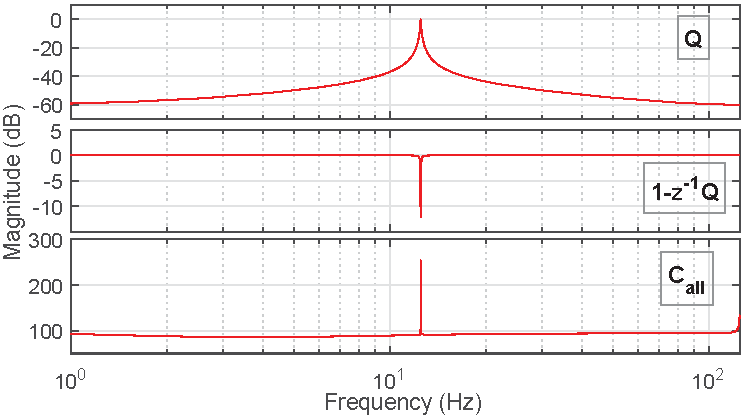
\includegraphics[width=13cm]{Loop-shaping/Q_and_one_minus_zinvQ_2}
\par\end{centering}
\caption{\label{fig:Magnitude-responses-of-LS}Magnitude responses of $Q(z)$,
$1-z^{-m}Q(z)$, and $C_{all}(z)$}
\end{figure}

Fig. \ref{fig:Output-of-the} shows the simulated outputs and control
efforts with the $Q$-filter and the baseline PID controller. The
results verify that compared with the baseline controller, the inverse-based
YK scheme can fully reject the disturbance at $12.5\,\text{Hz}$ with
increased control efforts.
\begin{figure}[!ht]
\begin{centering}
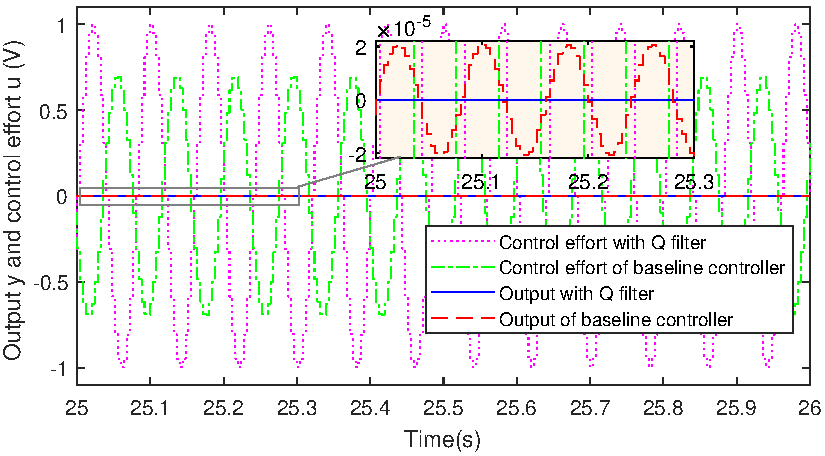
\includegraphics[width=13cm]{Loop-shaping/Q_output_3}
\par\end{centering}
\caption{\label{fig:Output-of-the}Outputs and control efforts of the baseline
controller and $Q$-filter}
\end{figure}

\subsection{\label{subsec:Experimentation}Experimentation}

Experiments are conducted on the galvo scanner platform \cite{wang2016spectral}
in Fig. \ref{fig:Schematic-of-hardware-LS}. During implementation,
nonlinearity effects such as slew rate limit and input saturation
are insignificant compared with the external disturbance and are thus
omitted. The control signal is limited to \textpm 10 V. The
system is subjected to broad-band random disturbances at a magnitude
of about 10 mV. The sampling time $T_{s}$ is $0.025\,\text{ms}$,
that is, the Nyquist frequency is $20\,\text{kHz}$. 

A pseudorandom binary sequence signal is used as an input to estimate
the plant model. Magnitude responses of the measured and identified
plants are shown in Fig. \ref{fig:Magnitude-response-of}. The identified
plant model is expressed as
\begin{gather}
P_{d}(z)=\frac{-0.001945z+0.03172}{z^{2}-1.955z+0.9703}.\label{eq:identified_P}
\end{gather}

One can observe that (\ref{eq:discrete_time_P}) and (\ref{eq:identified_P})
share the same structure and similar poles with some gain normalization,
which attests to the validity of the identified plant model. 
\begin{figure}[!ht]
\begin{centering}
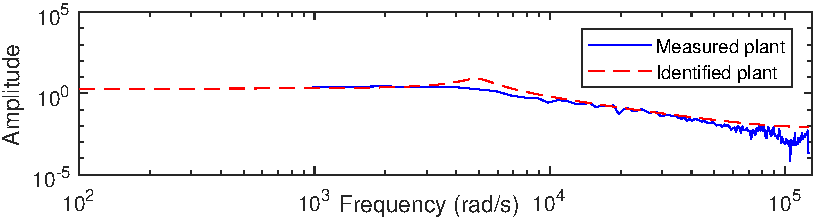
\includegraphics[width=13cm]{Loop-shaping/plant_estimation_tf_reduced}
\par\end{centering}
\caption{\label{fig:Magnitude-response-of}Magnitude response of the measured
and identified plant}
\end{figure}

Next, we take the galvo scanner and the servo drivers, namely, the
lumped plant and controller, as the new augmented plant $L(z)$ to
apply the outer-loop inverse-based YK parameterization in Fig. \ref{fig:A-outer-loop-inverse-based}.
The bandwidth $\omega_{c}$ of the baseline feedback loop is $1526\,\text{Hz}$,
as shown in Fig. \ref{fig:A-typical-magnitude}.
\begin{figure}[!ht]
\begin{centering}
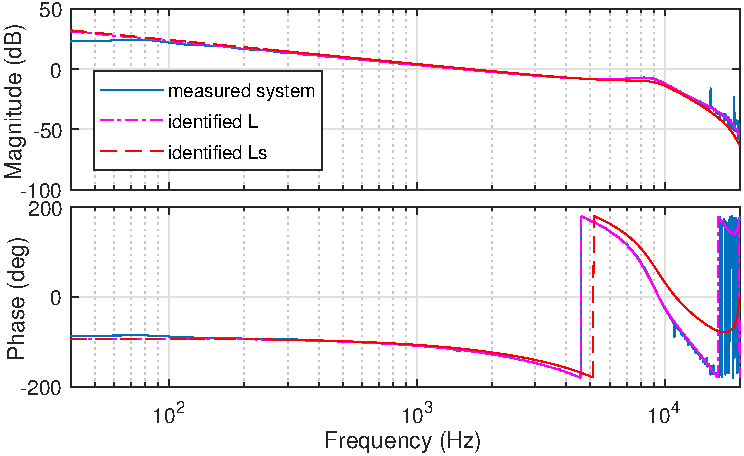
\includegraphics[width=13cm]{Loop-shaping/integrated_L_Ls_tf}
\par\end{centering}
\caption{\label{fig:Magnitude-response-of-1}Magnitude responses of the measured
system, and identified $\hat{L}(z)$, $\hat{L}_{s}(z)$ }
\end{figure}

The identified $\hat{L}(z)$ is
\begin{equation}
\hat{L}(z)=\frac{0.02816z^{2}+0.1504z+0.1146}{z^{4}-1.319z^{3}+0.929z^{2}-0.6073z-0.0035}.\label{eq:integrated_L}
\end{equation}

Moving the unstable zero of $\hat{L}(z)$ at $-4.419$ to $-0.6$
inside the unit circle and keeping the other zeros and poles unchanged
generates a new plant $\hat{L}_{s}(z)$ with a stable inverse $\hat{L}_{s}^{-1}(z)$
\begin{equation}
\hat{L}_{s}(z)=\frac{z^{2}+1.521z+0.5526}{10.49z^{4}-13.83z^{3}+9.037z-6.312z+0.6124}.\label{eq:integrated_L_stable}
\end{equation}

The magnitude responses of the measure system, the identified $\hat{L}(z)$,
and $\hat{L}_{s}(z)$ are very close to each other, as illustrated
in Fig. \ref{fig:Magnitude-response-of-1}. The $Q$-filter in Fig.
\ref{fig:A-outer-loop-inverse-based} is then designed based on the
inverse-stable plant $\hat{L}_{s}(z)$. The relative degree $m$ of
$\hat{L}_{s}(z)$ is 2. A disturbance with $f_{0}=5\,\text{kHz}$
and $A=0.1\,\text{V}$ is introduced to the system. $f_{0}$ at $5\,\text{kHz}$
is beyond the bandwidth $\omega_{c}$ ($1526\,\text{Hz}$) and cannot
be attenuated by the baseline feedback loop. Also, the Nyquist frequency
of $20\,\text{kHz}$ is large enough to obtain the frequency response
of the system at 5 kHz. Substituting $\alpha=0.9$ into (\ref{eq:singleQ_m_2})
gives
\begin{equation}
Q(z)=\frac{0.01-0.1414z^{-1}}{1-1.273z^{-1}+0.81z^{-2}}.\label{eq:singleQ_L}
\end{equation}

As shown in Fig. \ref{fig:System-output-with}, the control effort
with the $Q$-filter is larger than that with the baseline controller.
The disturbance is attenuated remarkably with the outer-loop inverse-based
YK parameterization turned on. The performance gain is also clear
in the frequency domain that as shown in Fig. \ref{fig:Spectrum-of-ooutput},
the spectral peak at 5 kHz is completely removed without visible amplification
of disturbances at the other frequencies.
\begin{figure}[!ht]
\begin{centering}
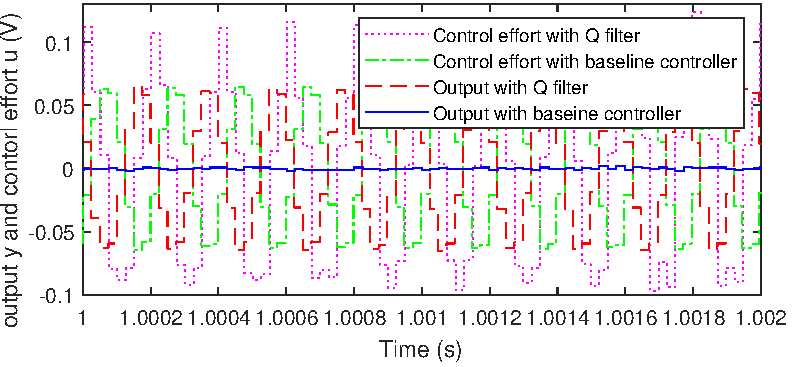
\includegraphics[width=13cm]{Loop-shaping/output_Q_baseline_2}
\par\end{centering}
\caption{\label{fig:System-output-with}System outputs and control efforts
with/without YK parameterization}
\end{figure}
\begin{figure}[!ht]
\begin{centering}
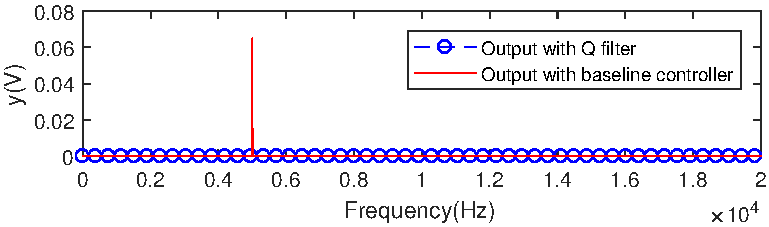
\includegraphics[width=13cm]{Loop-shaping/spectrum}
\par\end{centering}
\caption{\label{fig:Spectrum-of-ooutput}Spectrum of output $y(k)$}
\end{figure}

\section{Remarks}

\label{sec:comments}\emph{The plant model and its inverse}: The
(inverse) model information is essential in the discussed control
schemes since it not only provides convenience for feedback design
but also is beneficial for tasks such as fault detection and disturbance
isolation. Such a model is usually available in industries. By the
physical construction, the input to actuators in a precision positioning
system is usually a voltage/current signal that is approximately linear
with respect to motor torque, and the measurement is commonly an angular
or linear position. The inverse system dynamics thus usually has a
double-differentiator type of frequency response due to Newton's law.
It is thus not difficult to obtain a stable nominal $\hat{P}^{-1}(z)$
that accurately presents the low-frequency dynamics.\footnote{Friction can also be approximated by a second-order mode with damping
and spring.} Direct differentiation at high frequencies is not practical due to
high-frequency resonances. High-frequency unstable zeros, if any,
can be addressed by, for instance, shifting them inside the unit circle. A more systematic model inversion technique will be presented in Chapter \ref{chap:Model-Inversion}.

\emph{Robust stability}:\emph{ }Strictly speaking, after $\hat{P}$
is applied in the controller design, we are implementing a robust
version of YK parameterization. Notice that in the examples in Figs.
\ref{fig:A-loop-shaping} and \ref{fig:Q_wideband}, the $Q$-filters
are designed such that their magnitudes are small at high frequencies,
namely, the loop behavior at ultra-high frequencies does not change.
This is important for implementation, since it is practically impossible
to have an exact mathematical model for mechanical systems. The robust
stability analysis can give us upper bounds of the plant uncertainties
for the closed-loop system to maintain stable. Intuitively, flexible
loop shaping can be readily achieved at frequency regions where the
model $\hat{P}^{-1}(z)$ accurately reflects the actual system dynamics.
At high frequencies where the plant behavior itself cannot be well
predicted, the magnitude of $Q(z)$ (and hence the add-on control
efforts) is recommended to be kept small for robust stability. 

\emph{Feedforward control}: The feedback perspective for precision
servo has been discussed. Necessity
of FF control comes from the simple fact that feedback designs have
bandwidth limitations. In the FF class of control algorithms, model-based
design is also of essential importance. Inverse complementary sensitivity
and inverse plant dynamics are two common approaches for FF design.
When the process is repetitive, iterative learning control (ILC) is
another powerful tool for error correction in the iteration domain.\emph{}

\emph{Adaptive configuration}: When the disturbance spectra is not
known (but with known structure), adaptive control can be applied
to update the parameters of $Q(z)$ online. Investigation for the
case of narrow-band disturbance rejection is provided in the references
\cite{XuChen_TCST2012,chen2010unknown}.

\emph{Reference of YK parameterization}: For additional materials
about YK parameterization, readers can refer to references \cite{landau2005adaptive,doyle2013feedback,ANDERSON19981485}.
In the discrete-time case, the simplest example of $Q$ design is
using $Q(z)=\theta_{0}+\theta_{1}z^{-1}+\theta_{2}z^{-2}+...+\theta_{k_{Q}}z^{-k_{Q}}$,
namely, a finite impulse response (FIR) filter and then applying parameter
adaptation algorithms to find a set of $\theta_{i}$ that minimizes
the feedback error. This idea is also used in adaptive inverse control
\cite{Widrow2007}.

\section{Summary}

\label{sec:conclu}In this chapter, the control methodologies for precision
positioning systems have been studied. The central concept is that
flexible loop shaping is a convenient tool for addressing various
servo problems. Multiple simulation and experimental results on actual
engineering problems (e.g., the galvo scanner platform) are used to validate the presented designs. Besides
the examples given in this dissertation, the control structure has also
been tested under other systems, such as electrical power steering
in automotive vehicles \cite{chen2013inverse} and active suspension
systems \cite{chen2013selective,landau2005adaptive}. 

% ========== Chapter 7

\chapter{Fractional-order Repetitive Control} \label{chap:Fractional-RC}

\section{Introduction} \label{sec:Fractional-RC-Introduction}

Repetitive control (RC) \cite{inoue1981highpower} is designed to
track/reject periodic exogenous signals in applications with repetitive
tasks, as mentioned in Section \ref{subsec:repetitive-control}. By learning from memories of previous iterations in the repetitive
task, RC can drastically enhance current control performance in the
structured task space. Application examples include tracking controls
in magnetic and optical disk drives \cite{chew1989digital,doh2006design},
wafer scanners \cite{XuChen_TCST_RC2013}, and robotic manipulators
\cite{cosner1990plug,meng2017robust}, as well as regulation controls
in wind turbines \cite{navalkar2014subspace,castro2017variable},
power converters \cite{nazir2015analysis}, and unmanned aerial vehicles
\cite{he2017repetitive}.

This chapter studies RC in LPBF process (see, e.g., Figs. \ref{fig:Schematic-of-laser-scanning} and \ref{fig:Schematic-of-laser-scanning})
contains highly repetitive thermomechanical interactions \cite{carter2014influence,kruth2004selective,simchi2003effects}.
As a result, periodic errors are introduced in the laser-material
interaction and path planning. Indeed, such periodicity has been validated
and leveraged upon to improve control processes in other laser-based
AM technologies \cite{hoelzle2016spatial,lim2017multi,heralic2012height}. To fully release the capability of RC to fundamentally improve the
repetitive laser scanning in LPBF AM, the internal model principle
\cite{francis1975internal,hara1988repetitive} must be carefully
configured in the control design. In digital RC, an internal model
$1/(1-z^{-N})$ is implemented in the controller, where $N$ is the period
of the disturbance/reference. $N$ equals the sampling frequency (denoted
in this chapter as $1/T_{s}$ or $f_{s}$) divided by the fundamental
frequency ($f_{0}$) of the periodic signal. When $N$ is an integer,
the repetitive controller can generate high gains at the fundamental
frequency and its harmonics, yielding small gains in the error-rejection
dynamics to create the desired servo performances. When $f_{s}$ is
not divisible by $f_{0}$, that is, $N$ is not an integer, RC with
the rounded $N$ cannot target the aimed harmonic frequencies exactly,
resulting in degraded performances.

Several strategies exist to potentially address problems related to
fractional-order periods in RC. \cite{steinbuch2007design} and \cite{ramos2012power}
introduce high-order repetitive controllers with delay elements to
widen the high-gain regions around the harmonic frequencies. \cite{nakano1996elimination},
\cite{yao2013implementation}, and \cite{chen2013linear} employ
spatial repetitive controllers in a spatial domain to obtain time-invariant
disturbance periods. \cite{cao2002adaptive} and \cite{kurniawan2011adaptive}
propose adaptive RC schemes where the sampling rate is adjusted adaptively
to get an integer $N$. \cite{merry2011delay} proposes a delay-varying
repetitive controller that uses knowledge of the repetitive variable
to continuously adjust the time-varying delay. \cite{nazir2015analysis},
\cite{liu2017universal}, and \cite{zou2015frequency} design different
filters to approximate the fractional orders of delays. \cite{liu2016high}
uses a correction factor to correct the deviated poles of the fractional-order
repetitive controller.

Despite the existing literature, it remains not well understood how
to create RC \emph{exactly} at the harmonic frequencies in the presence
of fractional-order periods and how to systematically analyze the
closed-loop performances. To bridge these knowledge gaps, this chapter
aims at generating enhanced control efforts exactly at desired frequencies
in the fractional-order RC. The main result is the development of
a multirate RC algorithm and two indirect RC schemes. First, a wide-band
RC is achieved by applying the nearest integer of $N$ while widening
the attenuation width of each frequency notch in the error-rejection
dynamics. In the second indirect RC, a fictitious fundamental frequency
is introduced to get an integer $N$, which creates an overdetermined
rejection of the original repetitive errors. The proposed new multirate
RC designs the internal model under a second divisible fast sampling
frequency $f_{s}^{'}$ such that $N=f_{s}^{'}/f_{0}$ is an integer,
and embeds a new zero-phase low-pass filter design to address multirate
closed-loop robustness.

Along the course of formulating the multirate RC, an unexpected selective
loop-shape modulation is discovered in the intrinsic multirate digital
control design. This fundamental behavior, prone to be neglected in
the design phase, inspires in the first instance a closed-loop analysis
method that exhibits the complete disturbance-attenuation properties
of the multirate RC. This analysis method also enables a new design
space for applying RC to general systems with mismatched sampling
and task periodicity. The remainder of this chapter will discuss the
theoretical benefits, implementation guidance, and performance comparison
of the proposed algorithms. Theoretical analyses are verified by a
case study on a galvo scanner in LPBF.

The remainder of this chapter is structured as follows. Section \ref{sec:Repetitve-Control}
 reviews a RC design. Two examples in Section \ref{sec:Fractional-order-Disturbances}
elucidate the existence
of fractional-order disturbances in LPBF. Section \ref{sec:Proposed-Fractional-order-RC}
builds the proposed fractional-order RC algorithms. Section \ref{sec:Verification-Galvo-Scanner}
provides the numerical and experimental verification of the algorithms.

\section{Preliminaries of Repetitive Control} \label{sec:Repetitve-Control}

The proposed fractional-order RC algorithms are based on a plug-in
RC design in Fig. \ref{fig:Block-diagram-RC} \cite{XuChen_TCST_RC2013}.
Consider a baseline feedback system composed of the plant $P(z)$
and the baseline controller $C(z)$ (Fig. \ref{fig:Block-diagram-RC}
without the dotted box). $C(z)$ can be designed by means of common
servo algorithms, such as PID, $H_{\infty}$, and lead-lag compensation.
The signals $r(k)$, $e(k)$, $d(k)$, and $y_{d}(k)$ represent,
respectively, the reference, the tracking error, the input disturbance,
and the system output. Throughout the chapter, it is assumed that 1)
the coefficients of all transfer functions are real; 2) both $P(z)$
and $C(z)$ are rational, proper, linear, and time-invariant; 3) the
baseline feedback loop consisting of $P(z)$ and $C(z)$ is stable.

The plug-in compensator utilizes the internal signals $e(k)$ and
$u_{d}(k)$ to generate a compensation signal $w(k)$. Let $m$ denote
the relative degree of $P(z)$, whose nominal model is $\hat{P}(z)$.
With the plug-in compensator, the transfer function of the overall
controller from $e(k)$ to $u_{d}(k)$ is (\ref{eq:proposedYoula})

If $Q=(1-\alpha^{N})z^{m-N}/(1-\alpha^{N}z^{-N})$, that is,
\begin{equation}
1-z^{-m}Q(z)=\frac{1-z^{-N}}{1-\alpha^{N}z^{-N}},\label{eq:internal model}
\end{equation}

\noindent where $\alpha\in[0,\,1)$ is a tuning factor that determines
the attenuation bandwidth of $1-z^{-m}Q(z)$, then at the harmonic
frequencies ($\omega_{k}=k2\pi f_{0}T_{s}$, $k\in\mathbb{Z}^{+}$,
the set of positive integers), the magnitude responses of $1-z^{-m}Q(z)$
are zero because $1-\text{e}^{-j\omega_{k}N}=1-\text{e}^{-jk2\pi f_{0}T_{s}/(f_{0}T_{s})}=1-\text{e}^{-jk2\pi}=0$.
Hence, $|C_{all}(z)|\rightarrow\infty$ and $G_{d\rightarrow y_{d}}(z)=\frac{P(z)[1-z^{-m}Q(z)]}{1+P(z)C(z)}=0$
when $z=\text{e}^{j\omega_{k}}$. At the intermediate frequencies,
$Q(\text{e}^{j\omega})\approx0$, and $|1-z^{-m}Q(z)|_{z=\text{e}^{j\omega}}\approx1$
when $\alpha$ is close to 1; thus $C_{all}(z)\approx C(z)$, and
the original loop shape is maintained. Choosing a smaller $\alpha$
can yield a wider attenuation bandwidth, at the cost of deviating
from the baseline loop shape, as shown in Fig. \ref{fig:Q_wideband}.

Note that for $Q(z)$ in (\ref{eq:internal model}) to be implementable,
the disturbance period $N$ should be greater than the relative degree
$m$, which is commonly satisfied in sampled-data regulation control.
For instance, in the multirate RC example in Section \ref{sec:Verification-Galvo-Scanner},
$N=40>m=3$. Indeed, since the closed-loop bandwidth ($B_{p}$) is
designed to cover the fundamental disturbance frequency $f_{0}$ and
$B_{p}$ is no less than 10\% of the Nyquist frequency ($f_{s}/2$)
from principles of feedback design, common control practice thus renders
$N=f_{s}/f_{0}$ to be greater than 20. That is, $N$ is at least
one order of magnitude larger than the relative degree of the plant
model under principles of feedback design.

During implementation, zero-phase pairs $q_{j}(z^{-1})q_{j}(z)$ ($j\in\mathbb{Z}$)
are additionally incorporated into $Q(z)$ for robustness against
plant uncertainties at high-frequency regions:
\begin{equation}
Q(z)=\frac{(1-\alpha^{N})z^{-(N-m)}}{1-\alpha^{N}z^{-N}}\prod_{j=0}^{M}q_{j}(z^{-1})q_{j}(z),\label{eq:Qz_q0}
\end{equation}

\noindent where $M\in\mathbb{Z}$ is determined according to the design
requirements. For instance, the following design of $q_{i}(z)$ ($i\in\mathbb{Z}^{+}$)
places four zeros of $Q(z)$ at $\text{e}^{\pm j\Omega_{i}T_{s}^{'}}$
to make its frequency response equal zero at $\Omega_{i}$: 

\noindent 
\begin{equation}
q_{i}(z)=\frac{1-2\cos(\Omega_{i}T_{s})z+z^{2}}{2-2\cos(\Omega_{i}T_{s})}.\label{eq:q}
\end{equation}

\noindent 
\begin{equation}
q_{0}(z)=\frac{(1+z)^{n_{0}}}{2^{n_{0}}},\quad i=0.\label{eq:q-1}
\end{equation}

\noindent Here, $n_{0}\in\mathbb{Z}$ is the number of the added zero
pairs at the Nyquist frequency (Fig. \ref{fig:Magnitude-responses-of-2}). Note that the $Q$-filter in (\ref{eq:Qz_q0}),
(\ref{eq:q}), and (\ref{eq:q-1}) is designed assuming an integer
$N$ under the sampling time of $T_{s}$.

\begin{figure}[!ht]
\begin{centering}
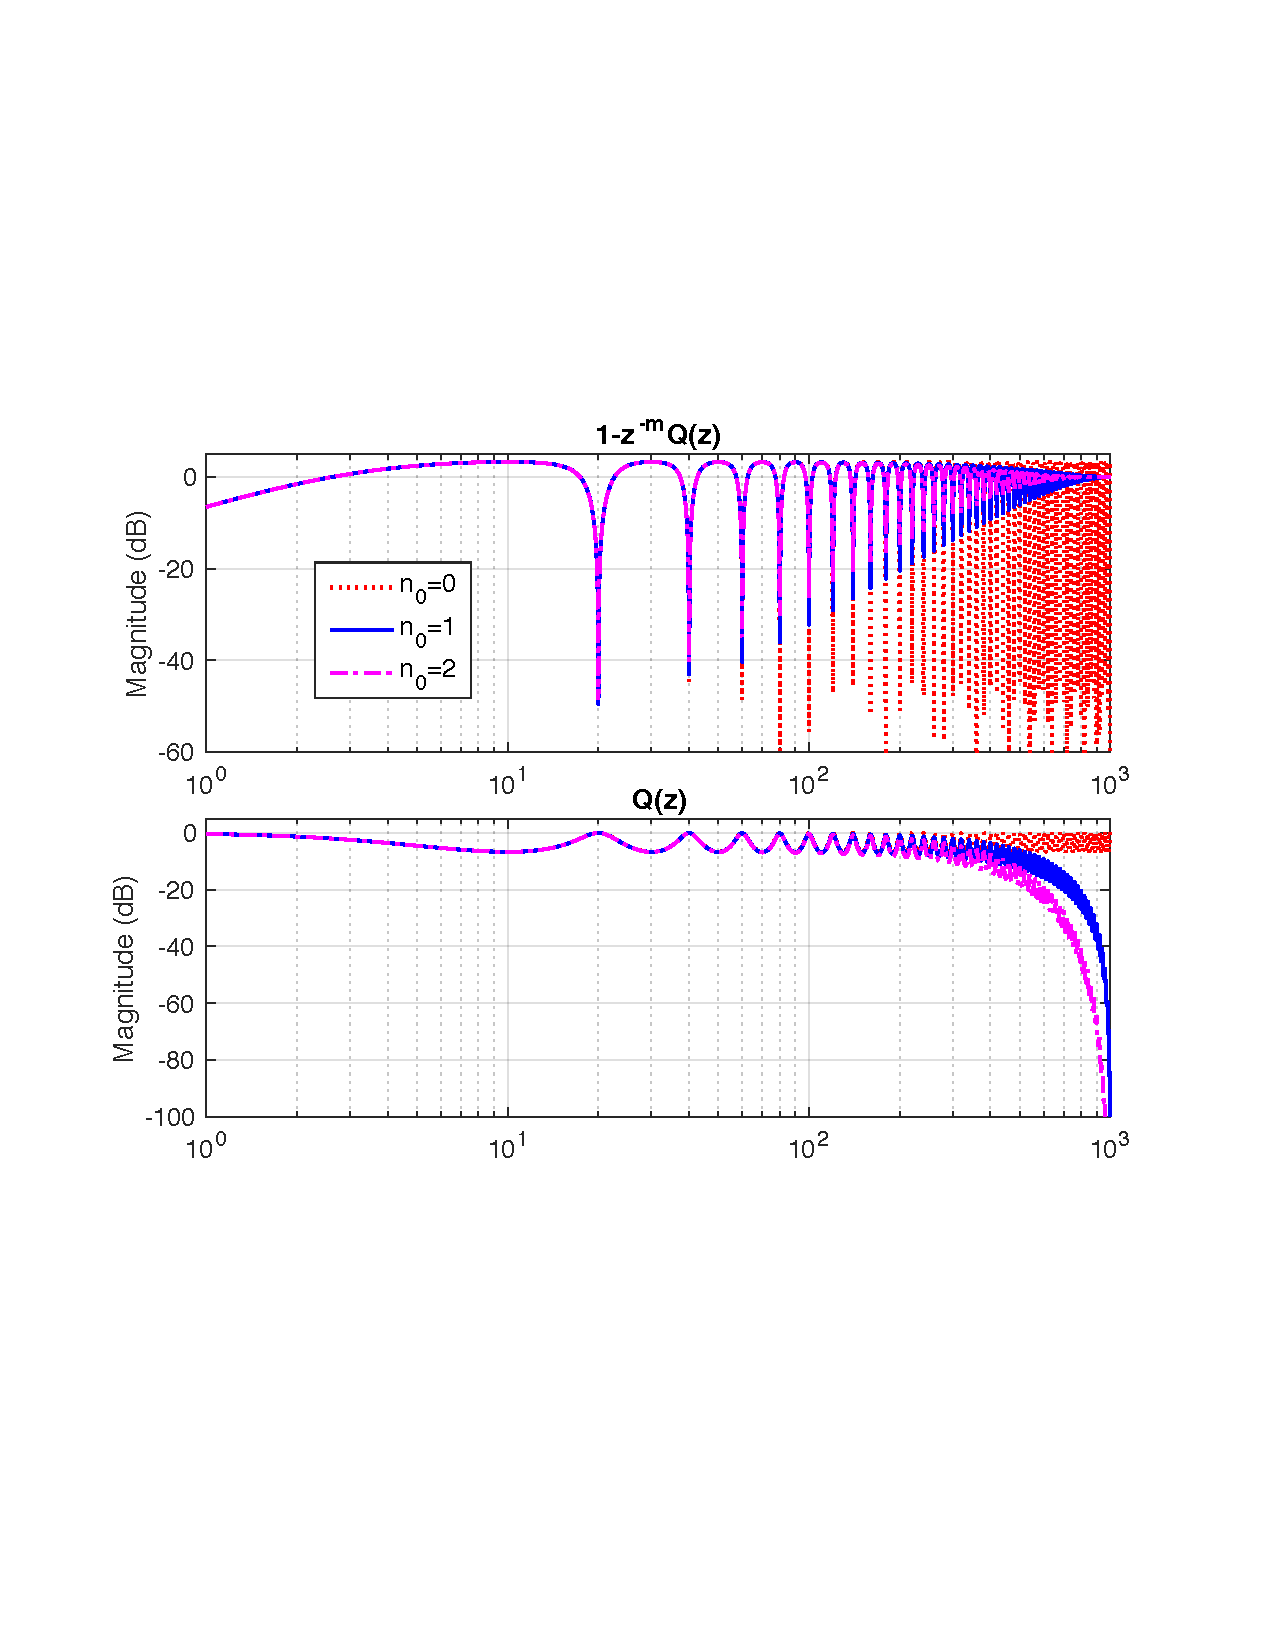
\includegraphics[clip,width=12cm]{Closed-loop-simulation/n0_threevalues_99}
\par\end{centering}
\centering{}\caption{\label{fig:Magnitude-responses-of-2}Magnitude responses of $1-z^{-m}Q(z)$
and $Q(z)$ with different $n_{0}$ (and $\alpha=0.99$) in an example
of Section \ref{chap:RC-Closed-loop-Simulation}.}
\end{figure}

\section{Fractional-order Disturbances in LPBF} \label{sec:Fractional-order-Disturbances}

This section motivates and justifies the application of fractional-order
RCs to the field of LPBF. In the first
example, fractional-order disturbances are observed to arise from
the laser scanning mechanism. Based on the periodic thermal cycles during the LPBF process, the second example verifies the existence of the fractional-order disturbances. 

\subsection{Collaborative Control in Galvo Scanner} \label{subsec:Collaborative-control-galvo-scanner}

The dual-axis galvo scanner in Fig. \ref{fig:Schematic-of-hardware-LS} is a
key component in LPBF for laser path planning. Typically, the dual-axis
galvo scanner consists of two sets of mirrors, motors, and control
systems, here referred to as the X channel and the Y channel, respectively.
With the collaborative rotation of the two mirrors, the input laser
beam is reflected to generate a predefined scanning trajectory at
high speed with high precision. The rotation angles of the mirrors
are measured by encoders mounted coaxially with the motor shaft in
the scanner enclosure.

In practice, periodic disturbances appear in the dual-axis galvo sets.
First, examine one single channel (e.g., Y channel) with a simple
harmonic signal $A\sin(2\pi f_{0}t+\phi)$. Frequency spikes at odd
multiples of $f_{0}$, instead of a single spike at $f_{0}$, show
up in the FFT of the channel output (Fig. \ref{fig:FFT-of-the-2}).
This is because signal conditioning boards in the servo driver limit
the rate of change in the output signal when the slope of the input
signal is faster than the predefined slew rate \cite{jung2005op}.
The slewed output waveform is thus not a pure sine waveform and results
in harmonics at odd multiples of the fundamental frequency.
\begin{figure}[!ht]
\begin{centering}
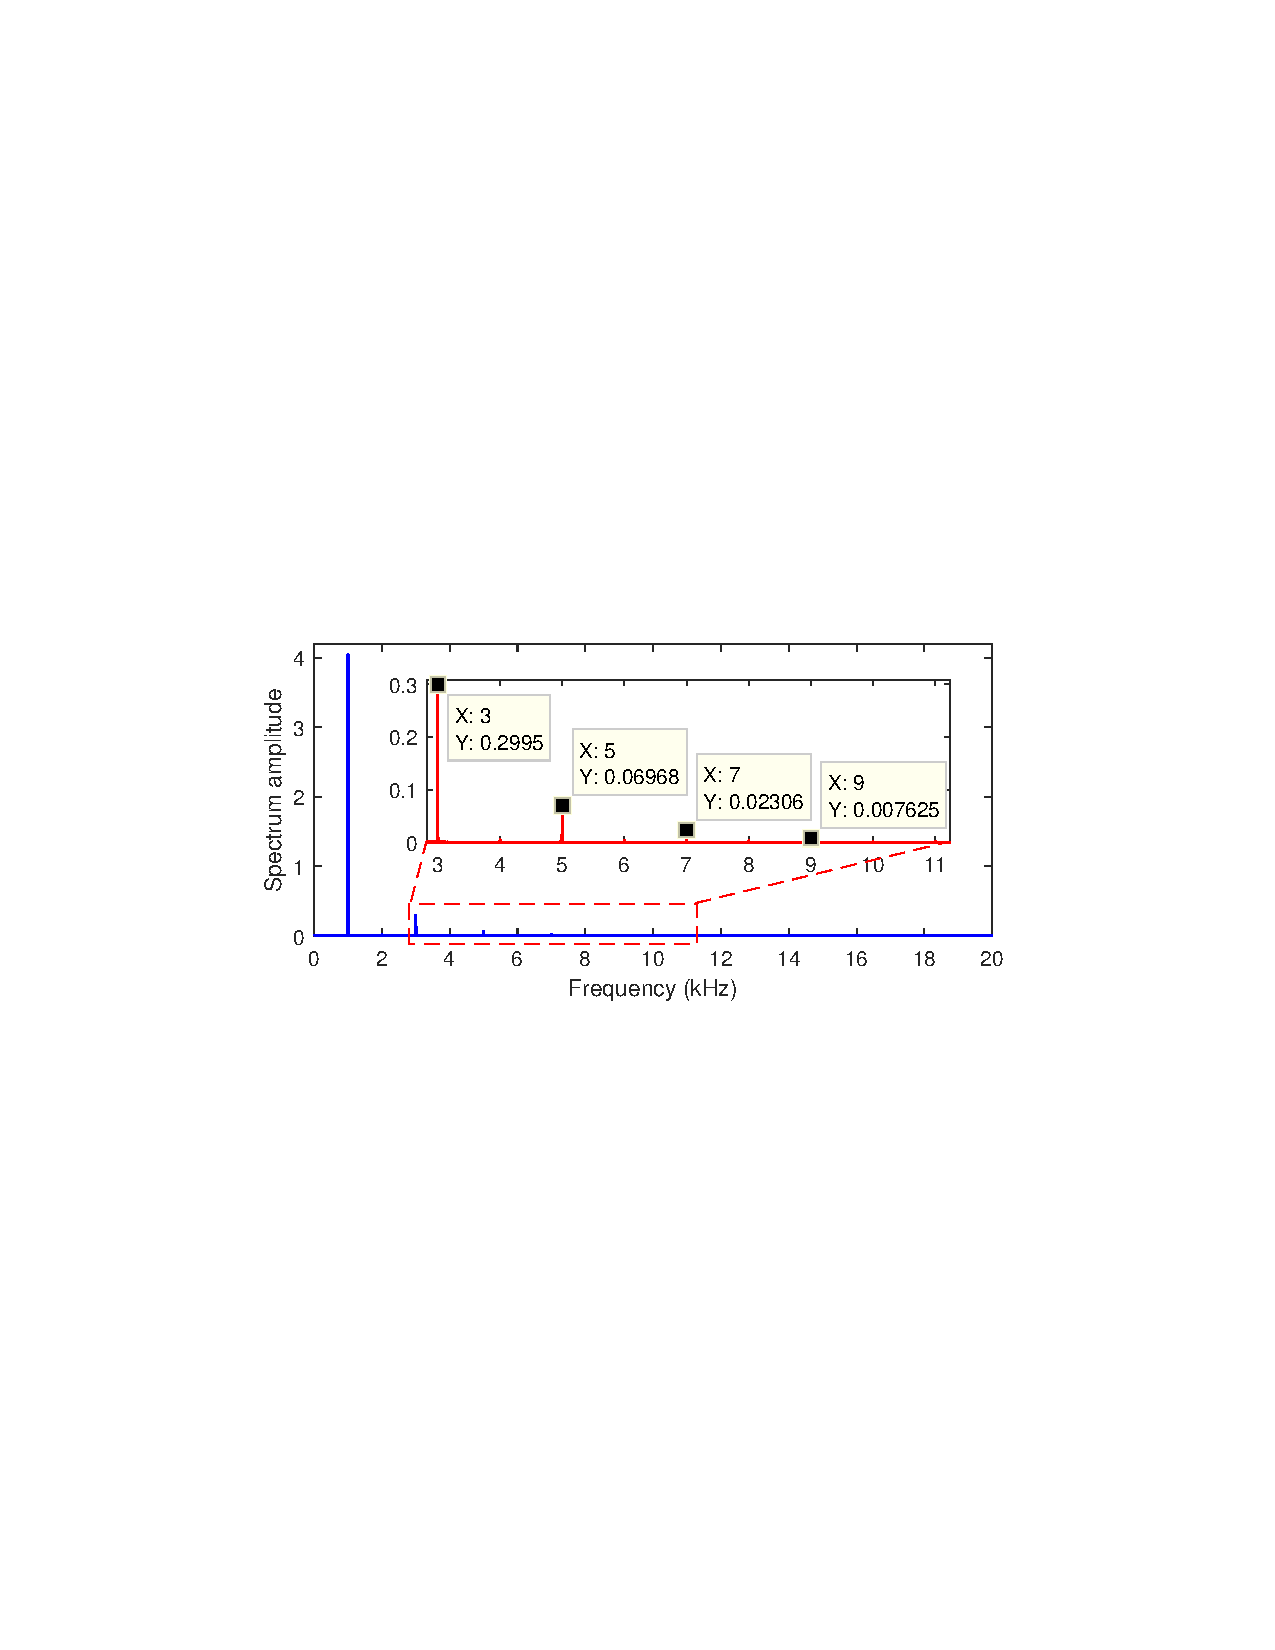
\includegraphics[width=13cm]{Fractional-order-RC/y_output}
\par\end{centering}
\caption{\label{fig:FFT-of-the-2}(Experimental result) FFT of the Y output
with a simple harmonic input.}
\end{figure}

Second, the collaborative control of the two channels also introduces
periodic disturbances. The mechanical motion of one rotating mirror
can transmit to the other mirror as disturbances. In addition, high
currents in the ground lines of the two servo drivers can cause the
channels to crosstalk \cite{Cambridge2008}. When actuating one channel
with a simple harmonic signal at $f_{0}$, the FFT of the non-actuated
channel output was observed to contain a frequency spike at $f_{0}$
caused by mechanical vibrations and frequency spikes at $2nf_{0}$
($n\in\mathbb{Z}^{+}$) due to crosstalk. Numerically, if the Y channel
is driven with a sine wave at 600 Hz and the X channel has no input,
frequency spikes at $1200\,\text{Hz}$, $2400\,\text{Hz}$, $3600\,\text{Hz}$,
etc arise at the FFT of the X output when the crosstalk is unaccounted
for. The crosstalk is more obvious with increased amplitudes $A$
and frequencies $f_{0}$ of the input signals (Fig. \ref{fig:FFT-of-the}).
\begin{figure}[!ht]
\begin{centering}
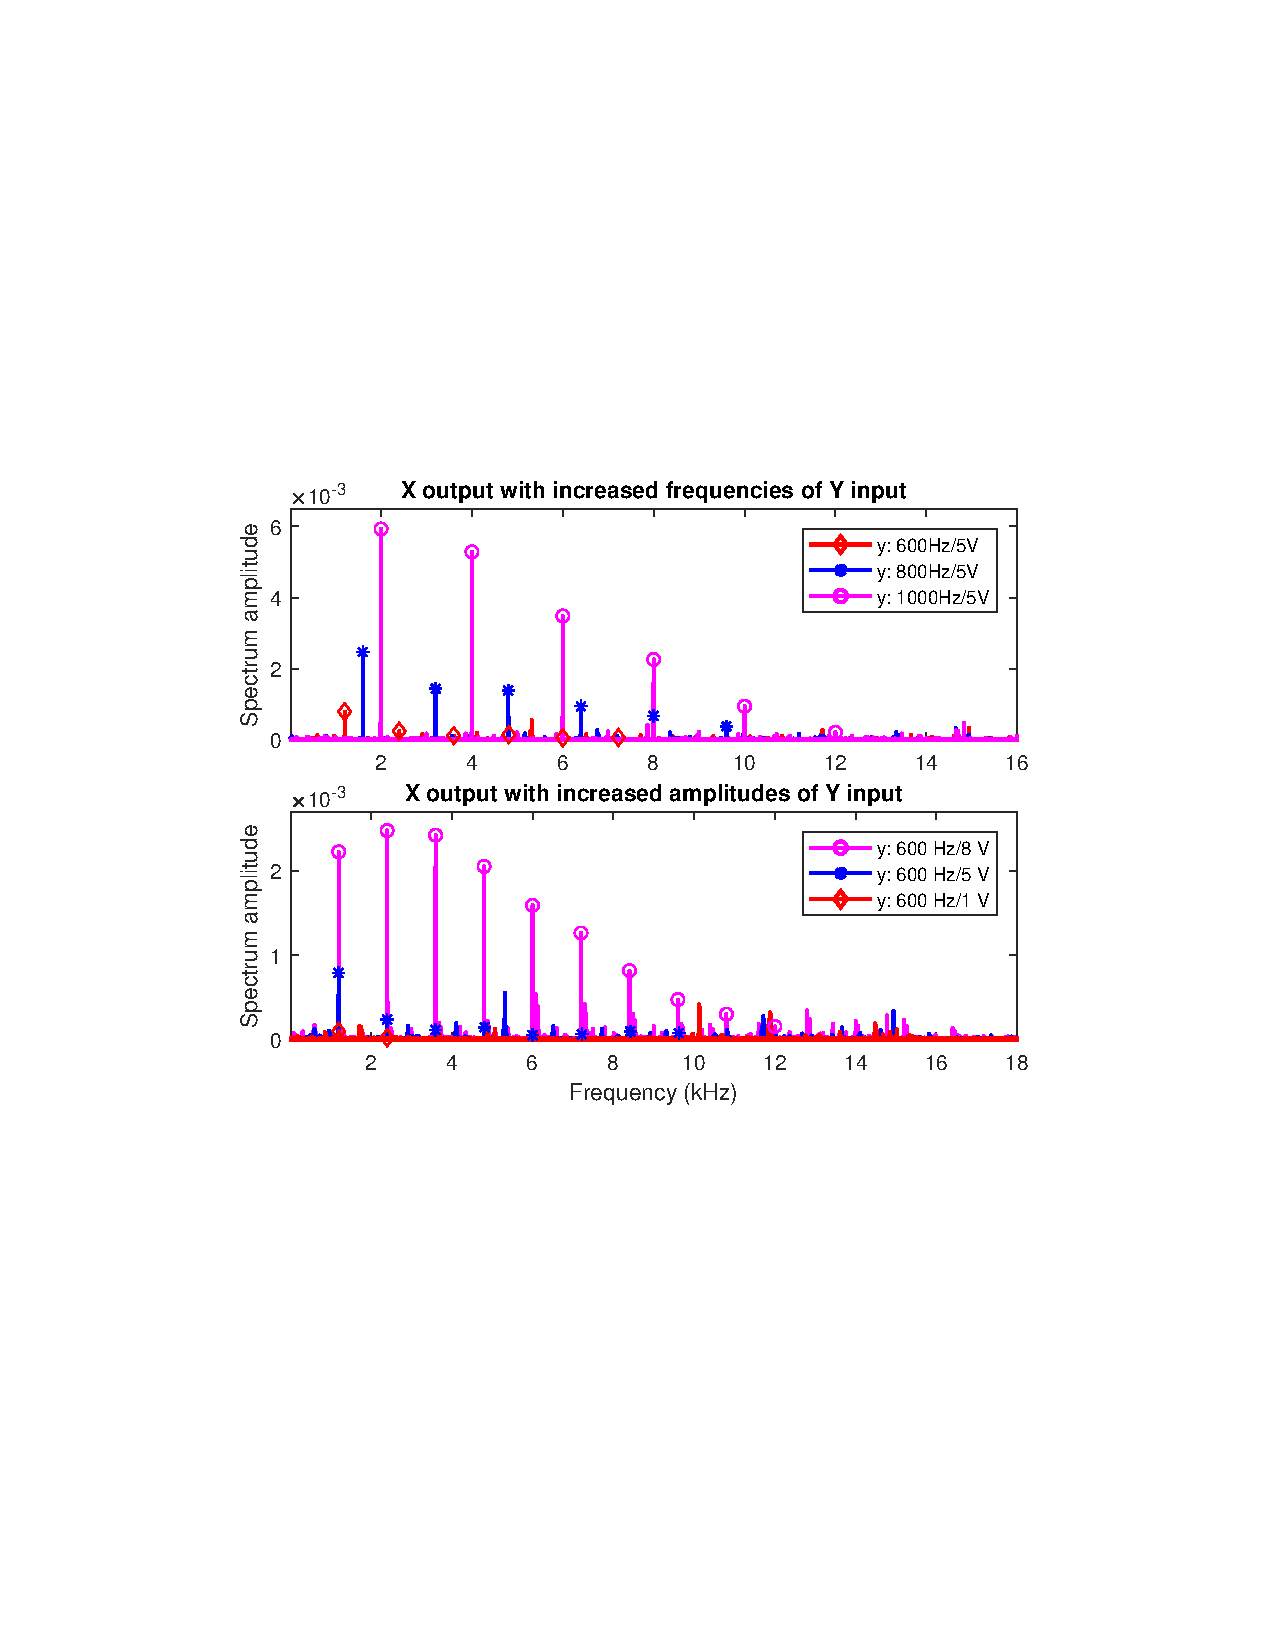
\includegraphics[width=13cm]{Fractional-order-RC/Increase_frequency_mag}
\par\end{centering}
\caption{\label{fig:FFT-of-the}(Experimental result) FFT of the X output with
increased frequencies and amplitudes of Y input.}
\end{figure}

For both single- and cross-channel disturbances, the disturbance frequencies
vary with the input signal frequencies and are not guaranteed to divide
the sampling frequency of the galvo scanner. For instance, when $T_{s}=1/16\,\text{ms}$,
conventional RC fails in eliminating the crosstalk-induced harmonics
at $\left\{ 1200i\,\text{Hz}\right\} \,(i\in\mathbb{Z}^{+})$ since
$N=16000/1200$ in the internal model is not an integer. Without loss
of generality, in this chapter, the proposed fractional-order RC algorithms
are evaluated on the dual-axis galvo scanner as a case study to reduce
the channel crosstalk.

\subsection{Periodic Thermal Cycles in LPBF} \label{subec:Periodic-thermal-cycles}

The LPBF is built upon repeated scanning of laser beam on a bed of
powder feedstock. The scan trajectories determine the periodicity
of the laser-material interactions (see, e.g., Fig. \ref{fig:Schematic-of-laser-scanning}).
Here, the laser beam melts the powder material following predefined
tracks, and monitoring sensors, such as cameras and imaging systems,
are applied to obtain the molten pool information. To get a uniform
part quality, the molten pool width is desired to be kept at a user-defined
reference value \cite{hofman2012camera}. On the one hand, periodic
disturbances are introduced into the LPBF process by the complex, repetitive
thermomechanical interactions, as shown in Section \ref{sec:Periodic-Thermal-Interactions}. On the other hand, because vision sensors
are restricted in changing sampling rates, the disturbance frequencies,
defined by laser path plannings, cannot always divide the sampling
frequencies of the monitoring sensors.

In the sample simulation in Section \ref{subsec:In-layer-Effects}, period $N(=f_{s}/f_{0}=50)$ is an integer
because $v/L$ divides $1/T_{s}$. However, the scan speed $v$ and
the track length $L$ are tailored to the required energy density
but not the speed of the monitoring sensors (which is restricted for
cameras and general integrated imaging systems). For instance, if
$T_{s}=3\,\text{ms}$, $N=100/3$ will become a non-integer. Therefore,
the disturbance periodicity—defined by the scan speed, the part geometry,
and the laser path planning—has no guarantees to be an integer multiple
of the sampling rate of the molten pool sensors. It is also important
to recognize that besides the proof-of-concept bidirectional trajectory,
other scanning patterns yield repetitive disturbance components in
a similar fashion (see, e.g., experimental results in \cite{dunbar2017comparisons}).
These fractional-order disturbances challenge conventional RC and
demand new algorithmic designs for RC to maximize performance in LPBF.

\section{Proposed Fractional-order RC Algorithms} \label{sec:Proposed-Fractional-order-RC}

Three algorithms are proposed to tackle a non-integer $N$ in the
RC internal model. Two indirect schemes, a wide-band RC and a quasi
RC, are first explored. Then the analyses and applications of the
main new multirate RC are developed. For concreteness, this section
will use the collaborative control example in Sections \ref{subsec:Collaborative-control-galvo-scanner}
and \ref{sec:Verification-Galvo-Scanner} throughout the discussions and
generalize the algorithms along the course of design and analysis.

\subsection{Wide-band and Quasi Repetitive Control} \label{subsec:Wide-band-and-quasi-RC}

The wide-band and quasi RC algorithms are two variants for directly
applying the conventional RC in (\ref{eq:proposedYoula}) and Fig. \ref{fig:Block-diagram-RC}
to the fractional-order cases. Both of them are implemented at the
baseline sampling time, namely, $T_{s}$. In the wide-band RC, $N$
is rounded to the nearest integer. Thus, high-control gains are generated
near the desired disturbance frequencies. To include these frequencies,
the wide-band RC chooses a smaller $\alpha$ to widen the attenuation
width of each frequency notch in $1-z^{-m}Q(z)$ , as shown in Fig.
\ref{fig:Q_wideband}. With $\alpha$ decreasing from 0.99 to 0.8,
the magnitude response of $1-z^{-m}Q(z)$ in Fig. \ref{fig:Zoom-in-magnitude-responses}
(a zoom-in view of Fig. \ref{fig:Q_wideband}) decreases from $-1.7\,\text{dB}$
to $-13\,\text{dB}$ at $1200\,\text{Hz}$, yielding increased control
efforts at the aimed frequencies. Although the wide-band RC cannot
perfectly reject the aimed disturbances, attenuation can be achieved
to some extent. As the attenuation width increases further, so does
the amplification of intermediate frequencies due to the waterbed
effect \cite{Bode1945}.
\begin{figure}[!ht]
\begin{centering}
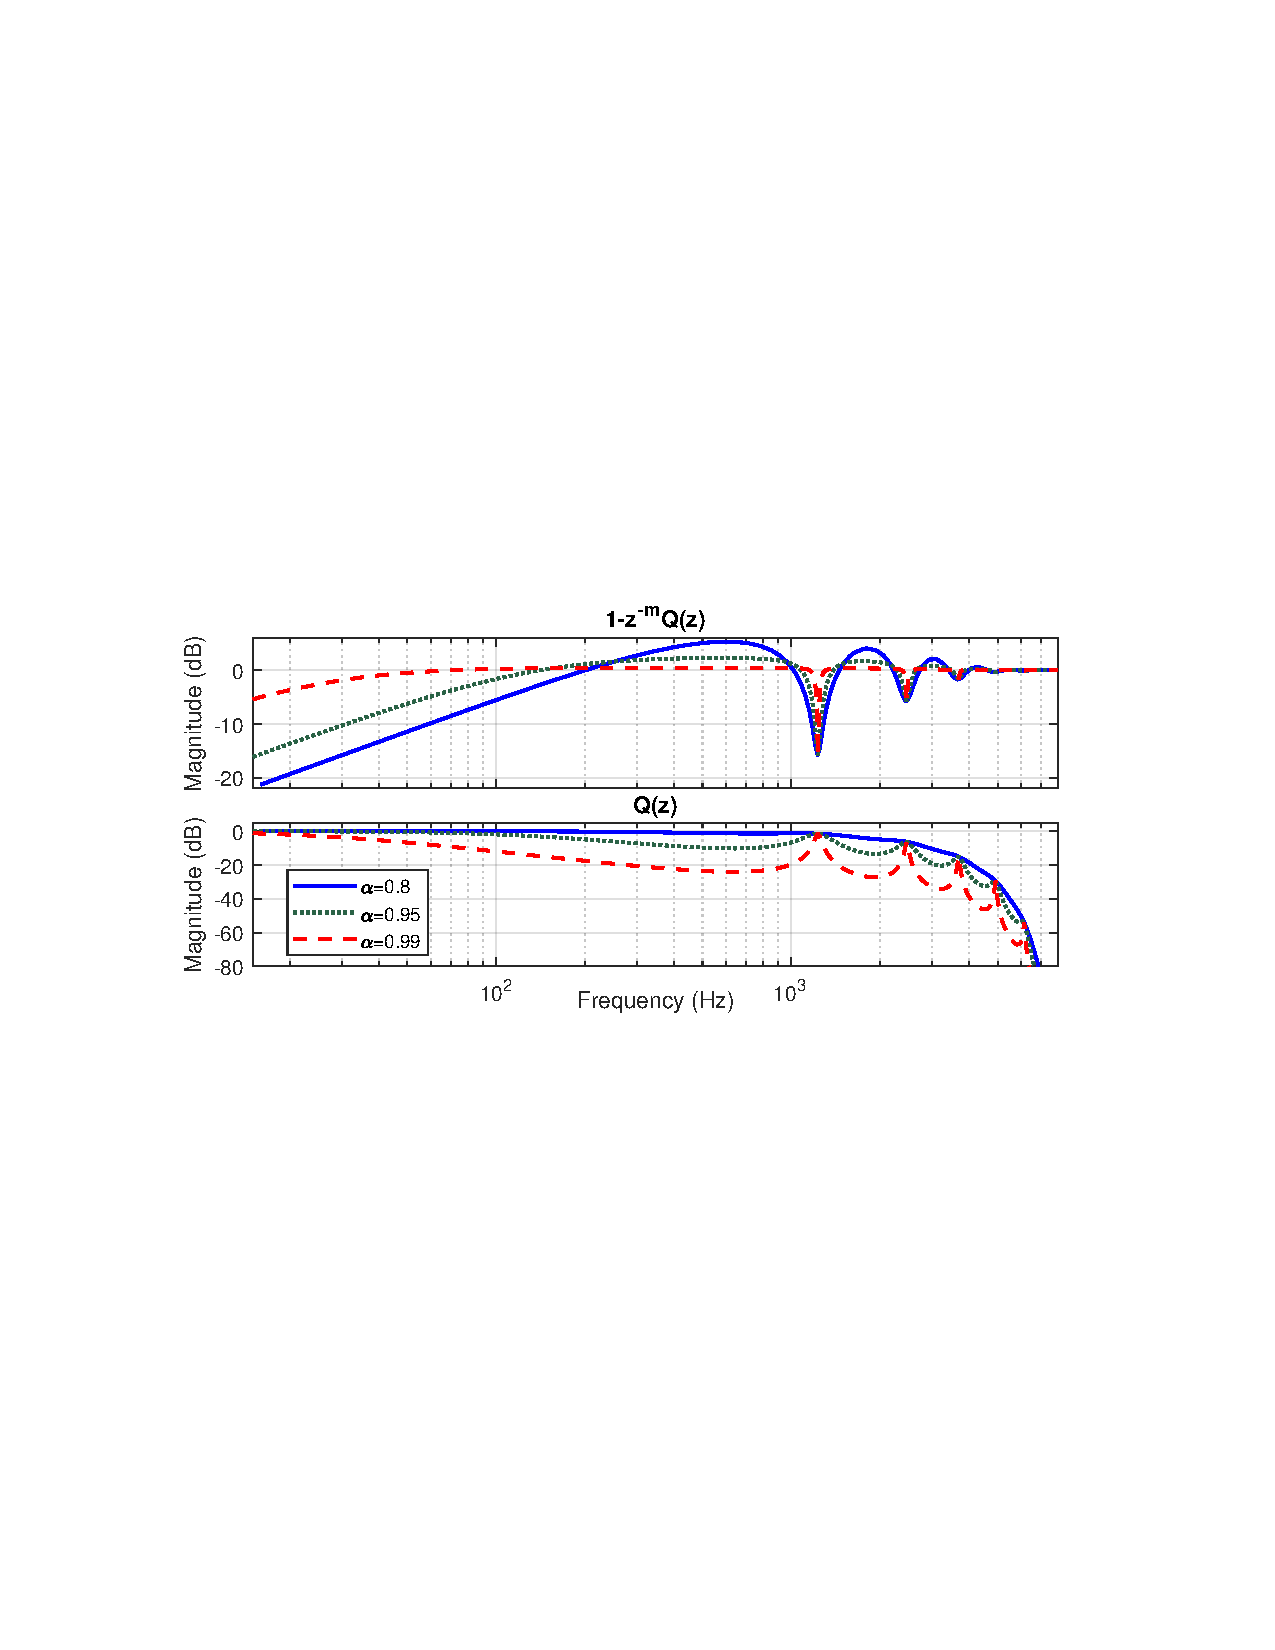
\includegraphics[width=14cm]{Fractional-order-RC/Q_wideband}
\par\end{centering}
\caption{\label{fig:Q_wideband}Magnitude responses of $1-z^{-m}Q\left(z\right)$
and $Q\left(z\right)$ in wide-band RC.}
\end{figure}
\begin{figure}[!ht]
\begin{centering}
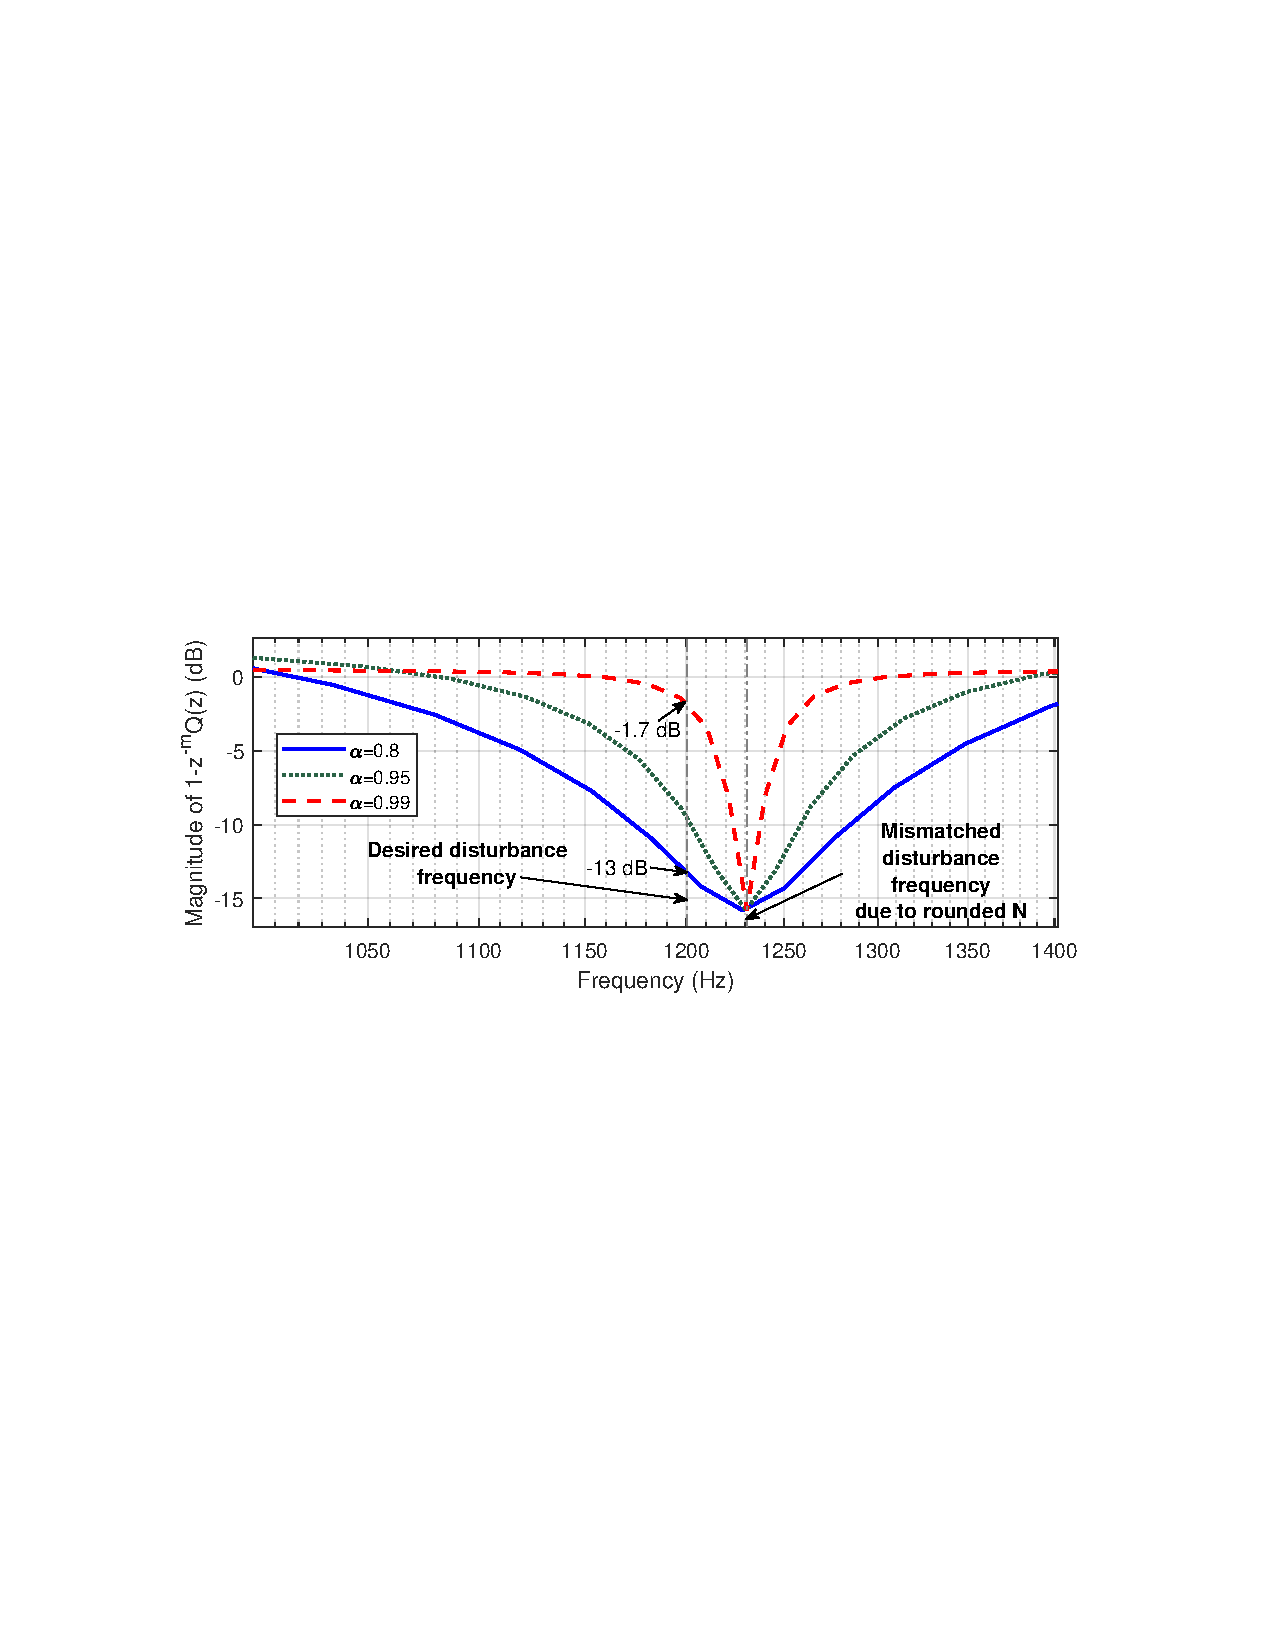
\includegraphics[width=14cm]{Fractional-order-RC/Q_wideband_zoomin}
\par\end{centering}
\caption{\label{fig:Zoom-in-magnitude-responses}Zoom-in magnitude responses
of $1-z^{-m}Q\left(z\right)$ in Fig. \ref{fig:Q_wideband}.}
\end{figure}

The proposed quasi RC designs an integer $N$ by introducing a fictitious
fundamental frequency that is the greatest common divisor (GCD) of
the fundamental and the sampling frequencies, namely, $N=f_{s}/\text{GCD}(f_{s},\,f_{0})$
and $f_{0}^{'}=\text{GCD}(f_{s},\,f_{0})=f_{s}/N$. In the example
from Section \ref{sec:Verification-Galvo-Scanner}, with $T_{s}=1/16\,\text{ms}$
and $f_{0}=1200\,\text{Hz}$, $N=16000/\text{GCD}(16000,\,1200)=40$,
and the fictitious fundamental frequency $f_{0}^{'}$ is $16000/40=400\,\text{Hz}$.
Quasi RC designed at $\left\{ 400i\,\text{Hz}\right\} \,(i\in\mathbb{Z}^{+})$
thus covers the desired harmonics at $\left\{ 1200i\,\text{Hz}\right\} \,(i\in\mathbb{Z}^{+})$
(with extra servo enhancement at $\left\{ 400i\,\text{Hz}\right\} \,(i,\,k\in\mathbb{Z}^{+}\,\text{and}\,i\neq3k$)),
as shown in Fig. \ref{fig:Q_quasi}. Note that $f_{0}^{'}$ must be
applicable for the quasi RC to work. For an example of $f_{0}=1220\,\text{Hz}$,
$f_{0}^{'}=\text{GCD}(16000,\,1220)=20$, and the control efforts
are largely wasted by generating high gains at many undesired frequencies
at $\left\{ 20i\,\text{Hz}\right\} \,(i,\,k\in\mathbb{Z}^{+}\,\text{and}\,i\neq61k$)).
\begin{figure}[!ht]
\begin{centering}
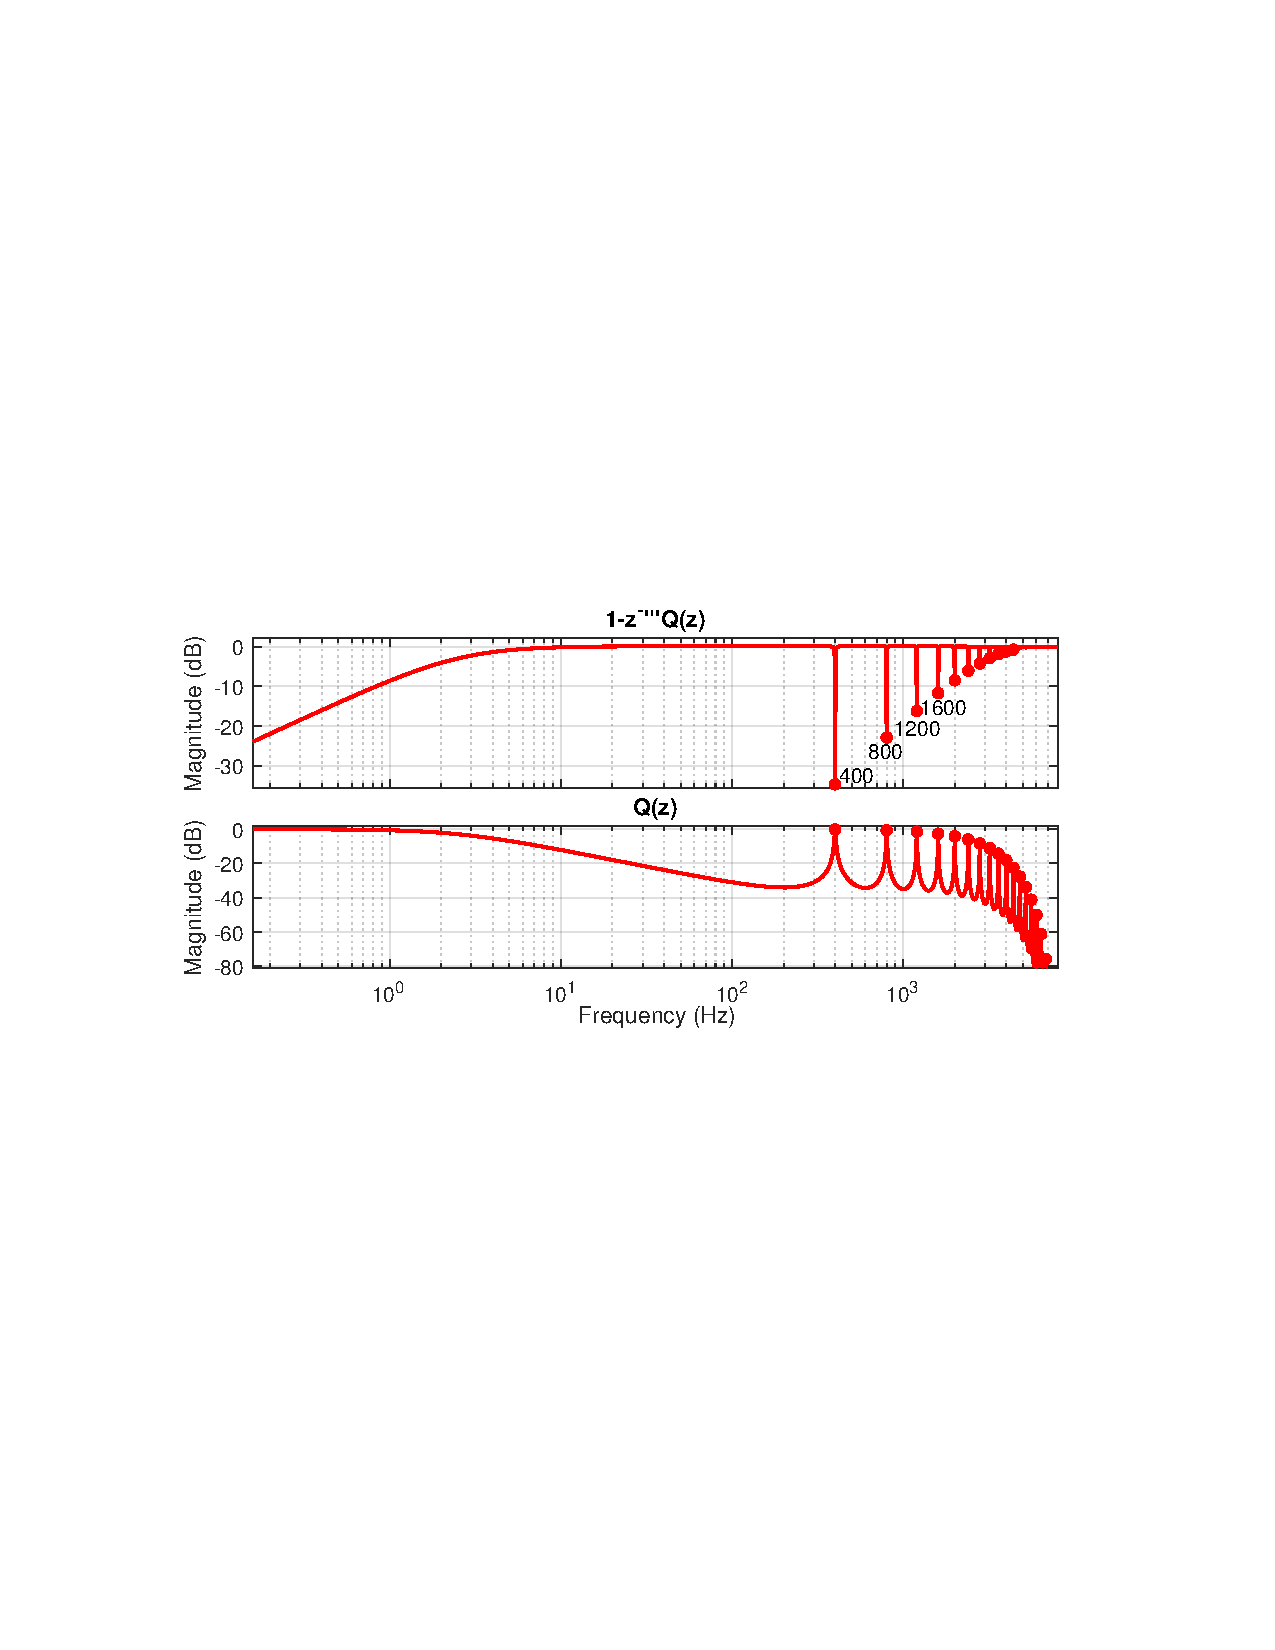
\includegraphics[width=14cm]{Fractional-order-RC/Q_quasi_RC}
\par\end{centering}
\caption{\label{fig:Q_quasi}Magnitude responses of $1-z^{-m}Q(z)$ and $Q(z)$
in quasi RC.}
\end{figure}

Inheriting from the plug-in RC design, the stability conditions for
the wide-band and quasi RCs are: $\hat{P}^{-1}(z),\,Q(z),\,\text{and }C(z)$
belong to the set of stable, proper, and rational transfer functions
\cite{XChen_ACC2013_tutorial}.

The wide-band RC and quasi RC are indirect solutions, only partially
attenuating the disturbances. For applications that require stronger
servo enhancement, more fundamental structural changes in the controller
design will be discussed next.

\subsection{Multirate Repetitive Disturbance Attenuation} \label{subsec:Multirate-RC}

The proposed multirate RC directly addresses the fractional-order
period by introducing a second divisible sampling frequency $f_{s}^{'}$.
Let $f_{s}^{'}$ equal the least common multiple (LCM) of the sampling
and fundamental frequencies, namely, $f_{s}^{'}=\text{LCM}(f_{s},\,f_{0})$.
Without changing the sampling frequency of the plant, the multirate
RC algorithm designs the repetitive controller with the internal
model under the newly introduced fast sampling frequency. Since $N=f_{s}^{'}/f_{0}$
is now an integer, the multirate repetitive controller can thus generate
high-gain control signals exactly at the fundamental frequency and
its harmonics.
\begin{figure}[!ht]
\begin{centering}
% \resizebox{12cm}{!}{%
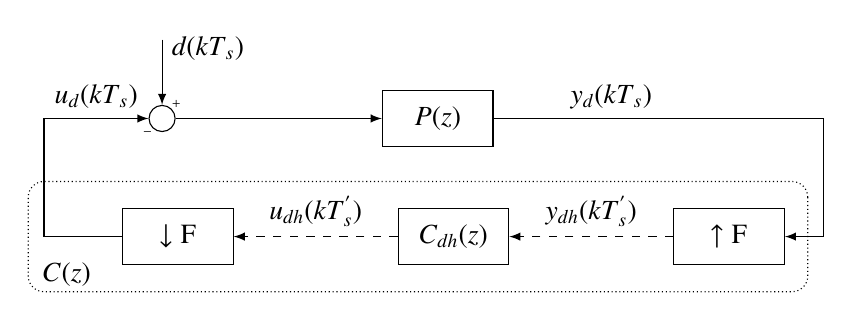
\begin{tikzpicture}[auto, node distance=3.5cm, >=latex] 

\node [input, name=input, xshift = 0.2cm] {}; 
\node [sum, right of=input, node distance=1.5cm] (sum) {}; 
\node [block, right of=sum] (plant) {$P(z)$};

\node [input, above of=sum, node distance=1cm](disturbance) {};
\draw [->] (disturbance) -- node [yshift = 0.3cm]{$d(kT_{s})$} node[pos=0.99] {\tiny $+$} (sum);

\node [coordinate, right of=plant, xshift = 0.2cm] (measurement1) {};
\node [block, below of=measurement1, node distance=1.5cm] (upsampling) {\text{$\uparrow$ F}};
\node [block, left of=upsampling] (controller) {$C_{dh}(z)$};
\node [block, left of=controller] (downsampling) {\text{$\downarrow$ F}};

\node [output, right of=measurement1, node distance=1cm, xshift = 0.2cm] (measurement2) {};

\draw [->] (input) -- node {$u_{d}(kT_{s})$} node[pos=0.99,below] {\tiny $-$} (sum);
\draw [->] (sum) -- (plant); 
\draw (plant) -- node {$y_{d}(kT_{s})$}(measurement1); 
\draw (measurement1) -- (measurement2);
\draw [->] (measurement2) |- (upsampling);
\draw [dashed, ->] (upsampling) -- node [above] {$y_{dh}(kT_{s}^{'})$}(controller);
\draw [dashed, ->] (controller) -- node [above] {$u_{dh}(kT_{s}^{'})$}(downsampling);
\draw (downsampling) -| (input);

\node [coordinate, xshift = -0.2cm, yshift = -0.8cm] (upperrightcorner) at (measurement2) {};
\node [coordinate, xshift = -0.2cm, yshift = -2.2cm] (lowerleftcorner) at (input) {};

\draw [densely dotted, rounded corners=.2cm] (upperrightcorner) rectangle (lowerleftcorner) node [above, pos = 0.9, xshift = -0.5cm, yshift = -0.2cm] {$C(z)$};
\end{tikzpicture}
% }
\par\end{centering}
\caption{\label{fig:Block-diagramPCH-with-1}Block diagram for multirate sampled-data
analysis.}
\end{figure}

Consider first a multirate sampled-data regulation control in Fig.
\ref{fig:Block-diagramPCH-with-1}, where the solid and dashed lines
represent the slow and fast signals sampled by $T_{s}$ and $T_{s}^{'}$($\triangleq1/f_{s}^{'}$),
respectively. $T_{s}^{'}$ and $T_{s}$ are related by $T_{s}^{'}=T_{s}/F$
($F>1$ and $F\in\mathbb{Z}^{+}$). The main elements here include
the plant $P(z)$, the controller $C_{dh}(z)$, the upsampler $\uparrow\text{F}$,
and the downsampler $\downarrow\text{F}$. Based on multirate signal
processing (see Appendix \ref{secA:Multirate-Signal-Processing}), the frequency response of the equivalent
feedback controller $C(z)$ in Fig. \ref{fig:Block-diagramPCH-with-1}
is
\begin{equation}
C(\text{e}^{j\Omega T_{s}})=\frac{1}{F}\sum_{k=0}^{F-1}C_{dh}(\text{e}^{j(\Omega T_{s}^{'}-\frac{2\pi k}{F})}).\label{eq:C}
\end{equation}

The proposed multirate RC (Fig. \ref{fig:Block-diagram-RC-1}) is
configured by inserting the upsampling and downsampling blocks into
Fig. \ref{fig:Block-diagram-RC} before and after the all-stabilizing
controller.
\begin{figure}[!ht]
\begin{centering}
% \resizebox{8.4cm}{!}{%
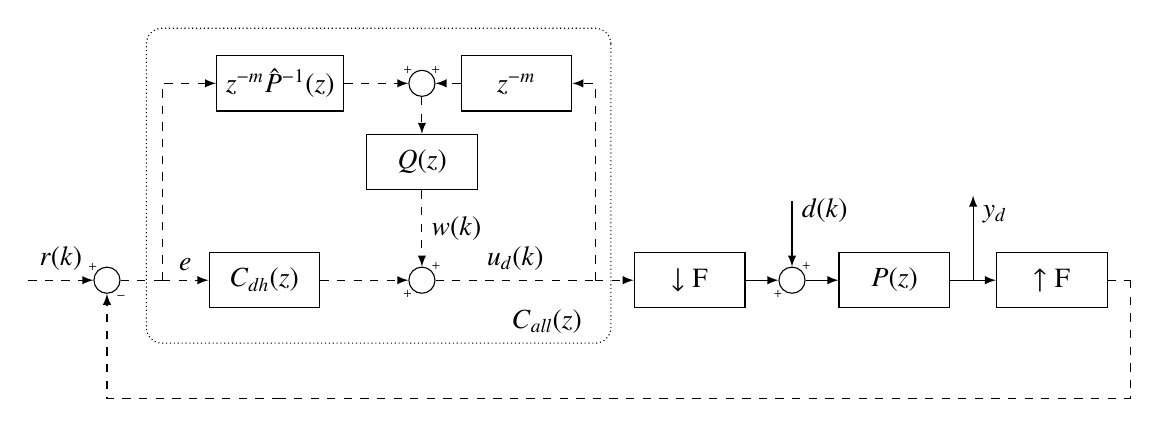
\begin{tikzpicture}[auto, node distance=2cm, >=latex] 
\node [input, name=input] {}; 
\node [sum, right of=input, node distance=1cm] (sum) {};
\node [coordinate, right of=sum, xshift = 0.2cm, node distance=0.5cm] (sumC) {};

\node [block, right of=sum] (controller) {$C_{dh}(z)$}; 
\node [sum, right of=controller] (sum2) {};
\node [coordinate, right of=sum2, xshift = 0.2cm] (sum2sum3) {};
\node [block, right of=sum2sum3, node distance=1.2cm] (downsampling) {$\downarrow$ F}; 

\node [sum, right of=downsampling, node distance=1.3cm] (sum3) {};
\node [block, right of=sum3, node distance=1.3cm] (plant) {$P(z)$};
\node [block, right of=plant] (upsampling) {$\uparrow$ F};

\node [output, right of=upsampling, node distance=1.0cm] (output) {};

\node [block, above of=sum2, node distance=1.5cm] (Q) {$Q(z)$};
\node [sum, above of=Q, node distance=1cm] (sum4) {};
\node [block, xshift = 0.2cm, left of=sum4] (Phat) {$z^{-m}\hat{P}^{-1}(z)$};
\node [block, right of=sum4, node distance=1.2cm] (Zm) {$z^{-m}$};

\node [coordinate, below of=controller, xshift = 0.2cm, node distance=1.5cm] (measurements) {};

\node [input, above of=sum3, node distance=1cm](disturbance) {};
\draw [->] (disturbance) -- node [yshift = 0.3cm]{$d(k)$} node[pos=0.99] {\tiny $+$} (sum3);

\draw [dashed, ->] (input) -- node {$r(k)$} node[pos=0.99] {\tiny $+$} (sum); 
\draw [dashed] (sum) -- (sumC); 
\draw [dashed, ->] (sumC) -- node {$e$} (controller);
\draw [dashed, ->] (controller) -- node[below, pos=0.99] {\tiny $+$} (sum2);
\draw [dashed](sum2) -- node {$u_{d}(k)$} (sum2sum3);
\draw [dashed, ->] (sum2sum3) -- (downsampling);

\draw [ ->] (downsampling) -- node[below, pos=0.99] {\tiny $+$} (sum3);

\draw [->] (sum3) -- (plant);
\draw [->] (plant) -- node [below] (PF) {} (upsampling);
\node [input, above of=PF, node distance=1.2cm](yd) {};
\draw [->] (PF) -- node [right, yshift = 0.3cm]{$y_{d}$}(yd);

\draw [dashed] (upsampling) -- (output);
\draw [dashed] (output) |- (measurements);
\draw [dashed, ->] (measurements) -| node[right, pos=0.99] {\tiny $-$}(sum);

\draw [dashed, ->] (sumC) |- (Phat);
\draw [dashed, ->] (Phat) -- node[pos=0.99] {\tiny $+$} (sum4);
\draw [dashed, ->] (sum4) -- (Q);
\draw [dashed, ->] (Q) -- node {$w(k)$} node[pos=0.99] {\tiny $+$} (sum2);
\draw [dashed, ->] (Zm) -- node[above, pos=0.99] {\tiny $+$} (sum4);
\draw [dashed, ->] (sum2sum3) |- (Zm);

\node [coordinate, xshift = 1.2cm, yshift = 0.7cm] (upperrightcorner) at (Zm) {};
\node [coordinate, xshift = -0.2cm, yshift = -0.8cm] (lowerleftcorner) at (sumC) {};

\draw [densely dotted, rounded corners=.2cm] (upperrightcorner) rectangle (lowerleftcorner) node [above, pos = 0.9, xshift = 4.5cm, yshift = -0.4cm] {$C_{all}(z)$};

\end{tikzpicture}
% }
\par\end{centering}
\caption{\label{fig:Block-diagram-RC-1}Block diagram for multirate RC.}
\end{figure}

The transfer functions inside the $C_{all}(z)$ block are implemented
at $T_{s}^{'}$. With the plug-in RC applied on top of $C_{dh}(z)$,
from (\ref{eq:C}), the frequency response of the open-loop transfer
function from $y_{d}$ to the summing junction before $P(z)$ is
\begin{equation}
\tilde{C}(\text{e}^{j\Omega T_{s}})=\frac{1}{F}\sum_{k=0}^{F-1}C_{all}(\text{e}^{j(\Omega T_{s}^{'}-\frac{2\pi k}{F})}),\label{eq:Yd-1}
\end{equation}

\noindent
\begin{equation}
C_{all}(\text{e}^{j\Omega T_{s}^{'}})=\frac{C_{dh}(\text{e}^{j\Omega T_{s}^{'}})+\text{e}^{-jm\Omega T_{s}^{'}}\hat{P}^{-1}(\text{e}^{j\Omega T_{s}^{'}})Q(\text{e}^{j\Omega T_{s}^{'}})}{1-\text{e}^{-jm\Omega T_{s}^{'}}Q(\text{e}^{j\Omega T_{s}^{'}})}.\label{eq:C-all-fre}
\end{equation}

Thus, when the reference $r(k)$ is zero (i.e., in regulation problems),
block diagram manipulations in Fig. \ref{fig:Block-diagram-RC-1}
give the Fourier transform of the plant output $y_{d}(k)$
\begin{eqnarray}
Y_{d}(\text{e}^{j\Omega T_{s}}) & = & \frac{P(\text{e}^{j\Omega T_{s}})D(\text{e}^{j\Omega T_{s}})}{1+\frac{1}{F}P(\text{e}^{j\Omega T_{s}})\sum_{k=0}^{F-1}C_{all}(\text{e}^{j(\Omega T_{s}^{'}-\frac{2\pi k}{F})})}\nonumber \\
 & = & \frac{P(\text{e}^{j\Omega T_{s}})D(\text{e}^{j\Omega T_{s}})}{1+P(\text{e}^{j\Omega T_{s}})\tilde{C}(\text{e}^{j\Omega T_{s}})}.\label{eq:Yd}
\end{eqnarray}

Before discussing the detailed full multirate closed-loop properties,
the authors provide a conceptual example and an overall disturbance-attenuation
principle. Consider again $T_{s}=1/16\,\text{ms}$ and $f_{0}=1200\,\text{Hz}$.
Multirate RC gives $T_{s}^{'}=\text{1/LCM}(16000,\,1200)=1/48\,\text{ms}$.
The plug-in compensator is designed under the sampling time of $T_{s}^{'}$
such that small gains of $1-z^{-m}Q(z)$ are generated at the harmonic
frequencies of $\Omega_{0}=2\pi n\times1200\,\text{rad/s}$ ($n\in\mathbb{Z}^{+}$),
as shown in Fig. \ref{fig:Q_multirate}. For disturbances at $\Omega_{0}$,
since the $Q$-filter design in Section \ref{sec:Repetitve-Control} gives
$C_{all}(\text{e}^{j\Omega_{0}T_{s}^{'}})\rightarrow\infty$, the
summation form of $C_{all}$ in (\ref{eq:Yd-1}) also goes to infinity.
Thus, in (\ref{eq:Yd}), $Y_{d}(\text{e}^{j\Omega_{0}T_{s}})\rightarrow0$,
yielding $y_{d}(kT_{s})=0$ at $\Omega_{0}$.
\begin{figure}[!ht]
\begin{centering}
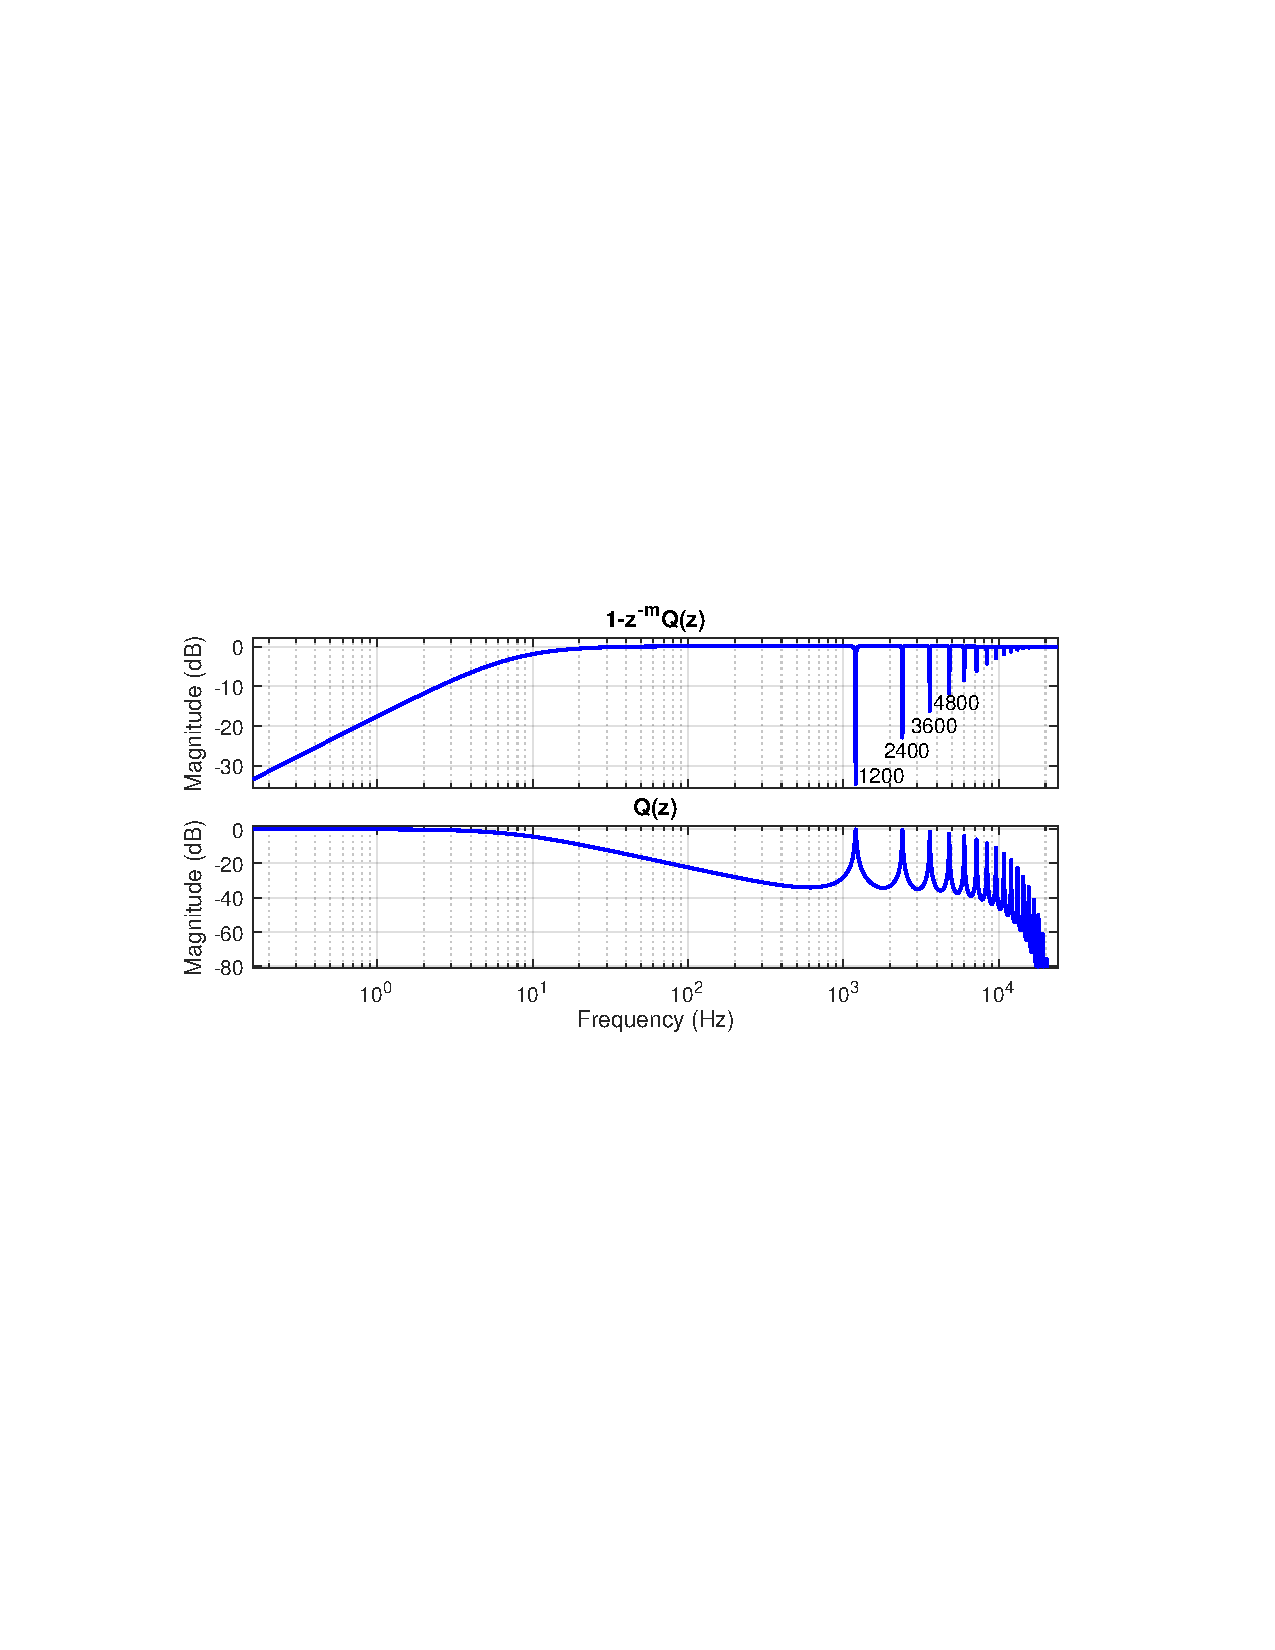
\includegraphics[width=13cm]{Fractional-order-RC/Q_multirate_RC}
\par\end{centering}
\caption{\label{fig:Q_multirate}Magnitude responses of $1-z^{-m}Q(z)$ and
$Q(z)$ in multirate RC.}
\end{figure}

\emph{Remark}: The proposed algorithm targets exact transformation
of the closed loop to formulate an integer parameter of the disturbance
period in the internal model, and thereby generates high control gains
exactly at the disturbance frequencies. As a trade-off, additional
computation is required to facilitate the multirate signal processing.
Under certain pairs of disturbance frequency and sampling rate of
the system, previous approximate RCs may work more economically under
the available computation budget. For instance, when $f_{0}=1199\,\text{Hz}$
and $T_{s}=1/16\,\text{ms}$, then $\text{LCM}(1/T_{s},\,f_{0})=\text{LCM}(16000,\,1199)=1918.4\,\text{kHz}$
is orders of magnitude larger than the original sampling rate, resulting
in high computation load that may be cost prohibitive on certain embedded
platforms.

\subsubsection{Multirate Closed-loop Analysis} \label{sssec:Multirate-closed-loop-analysis}

In Fig. \ref{fig:Block-diagram-RC-1}, the transfer function from
the disturbance $d(k)$ to the output $y_{d}(k)$ equals $S(z)=S_{0}(z)P(z)$,
where $S_{0}(z)$ is the closed-loop sensitivity function:
\begin{equation}
S_{0}(\text{e}^{j\Omega T_{s}})=\frac{1}{G(\text{e}^{j\Omega T_{s}})},\label{eq:S}
\end{equation}

\noindent and
\begin{equation}
G(\text{e}^{j\Omega T_{s}})=1+\frac{1}{F}P(\text{e}^{j\Omega T_{s}})\sum_{k=0}^{F-1}C_{all}(\text{e}^{j(\Omega T_{s}^{'}-\frac{2\pi k}{F})}).\label{eq:G}
\end{equation}

To reject disturbances at $\Omega_{0}$, when the plant dynamics
is fixed, $|S_{0}(\text{e}^{j\Omega_{0}T_{s}})|$ in the multirate
RC is desired to be small at $\Omega_{0}$, that is, $|G(\text{e}^{j\Omega_{0}T_{s}})|\rightarrow\infty$.
With the direct $Q$-filter design under the sampling time of $T_{s}^{'}$
(Fig. \ref{fig:Q_multirate}), $|S_{0}(\text{e}^{j\Omega T_{s}})|$
has the desired small gains at the target frequencies, as discussed
in the paragraph after (\ref{eq:Yd}). However, small spikes also
appear in $|S_{0}(\text{e}^{j\Omega T_{s}})|$, that is, decreasing
notches show up in $|G(\text{e}^{j\Omega T_{s}})|$ (Fig. \ref{fig:Sensitivity_func}).
The undesired selective small gains imply potential amplification
of other error sources. The complete disturbance-attenuation properties
of the proposed multirate RC will be deciphered next to assist in
eliminating those error amplifications.
\begin{figure}[!ht]
\begin{centering}
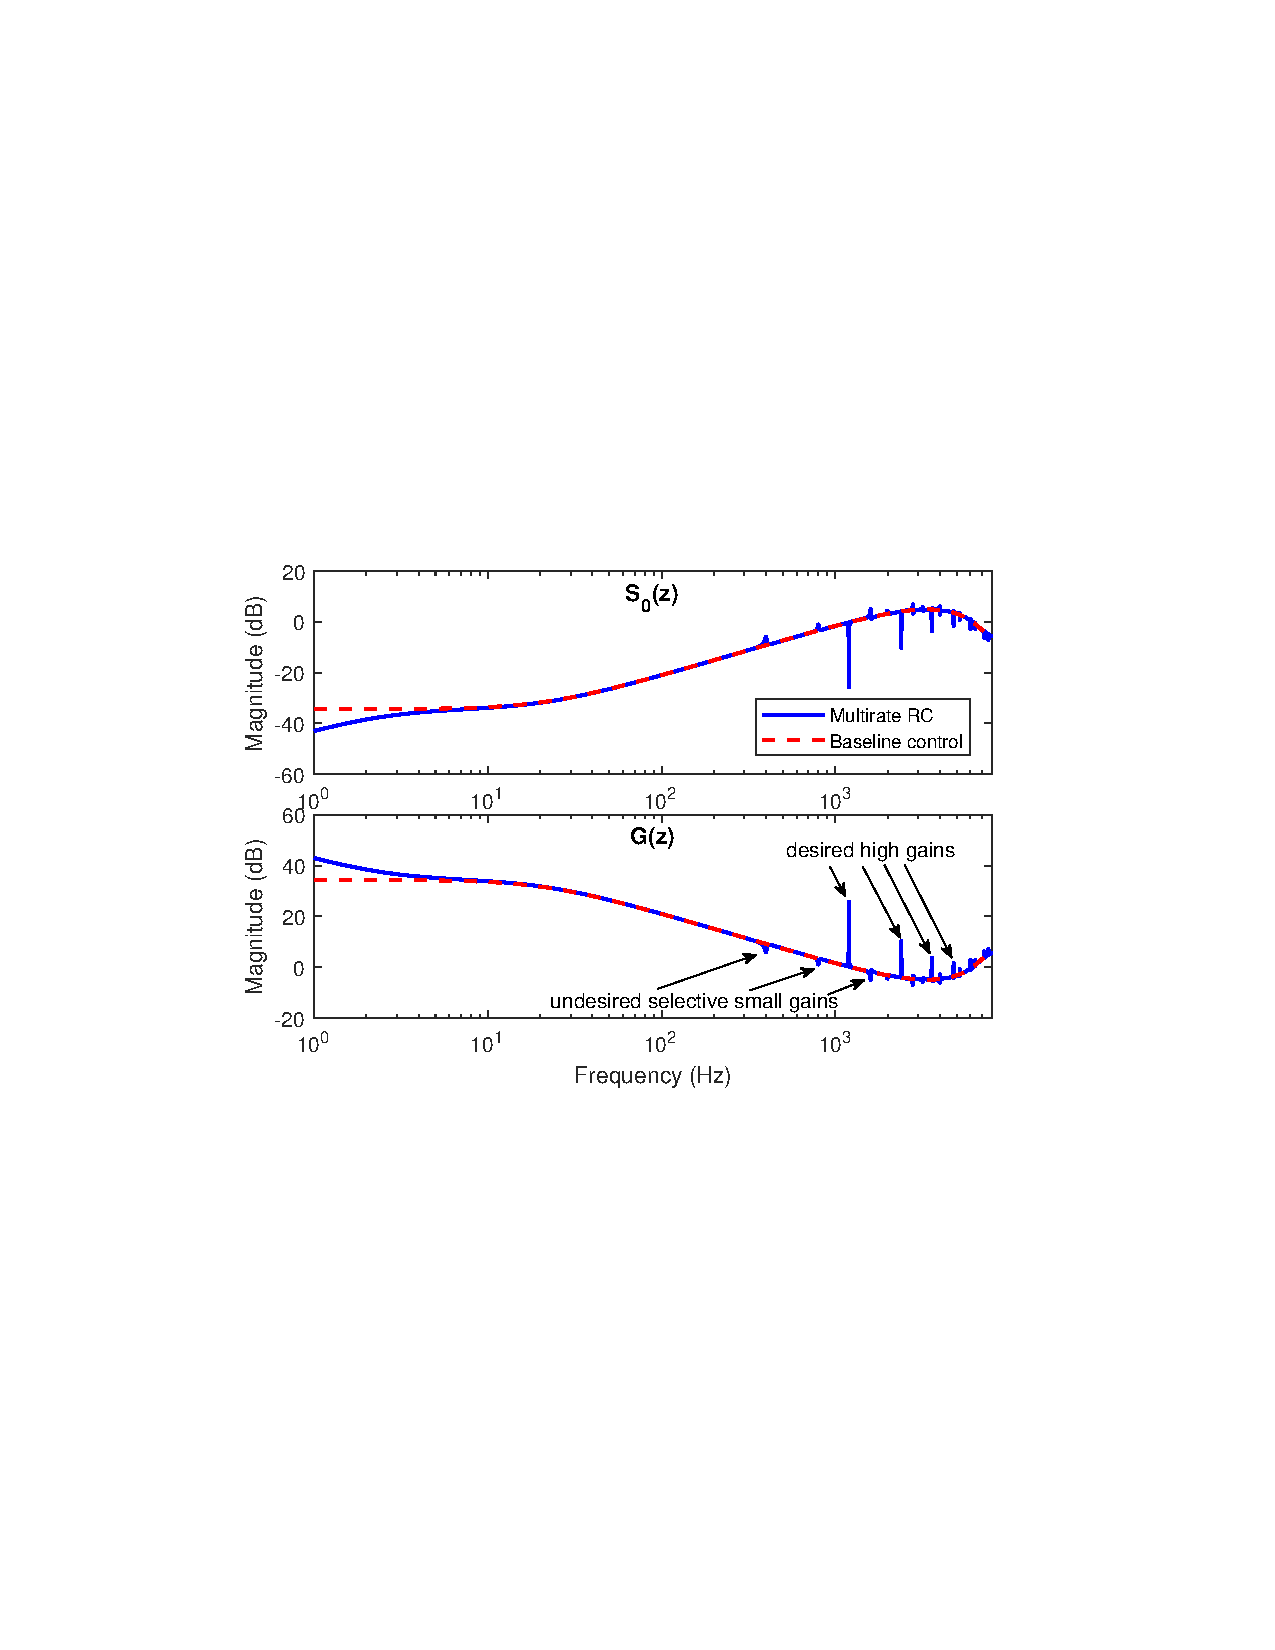
\includegraphics[width=11cm]{Fractional-order-RC/sensitivity_func_G_normalized}
\par\end{centering}
\caption{\label{fig:Sensitivity_func}Frequency responses of $S_{0}(z)$ and
$G(z)$ in Multirate RC with $T_{s}=1/16\,\text{ms}$, $T_{s}^{'}=1/48\,\text{ms}$,
$F=3$, and $f_{0}=1200\,\text{Hz}$. }
\end{figure}

Note that $G(\text{e}^{j\Omega T_{s}})$ in (\ref{eq:G}) contains
hybrid frequency responses of $P(z)$ under the sampling time of $T_{s}$
and $C_{all}(z)$ under $T_{s}^{'}$, and the frequency index satisfies
the periodicity property:
\begin{equation}
\text{e}^{j(\Omega T_{s}^{'}-\frac{2\pi k}{F})}=\text{e}^{j(\Omega-\frac{2\pi k}{T_{s}})T_{s}^{'}}=\text{e}^{j2\text{\ensuremath{\pi}}(f-\frac{k}{T_{s}})T_{s}^{'}},\label{eq:G-1}
\end{equation}

\noindent where $f=\Omega/(2\pi)$ is in Hz. Take the previous example
($T_{s}=1/16\,\text{ms}$, $T_{s}^{'}=1/48\,\text{ms}$, and $F=T_{s}/T_{s}^{'}=3$).
Then
\begin{equation}
G(\text{e}^{j2\pi fT_{s}})=1+\frac{1}{3}P(\text{e}^{j2\pi fT_{s}})\sum_{k=0}^{2}C_{all}(\text{e}^{j2\text{\ensuremath{\pi}}(f-\frac{k}{T_{s}})T_{s}^{'}}).\label{eq:G_F_3}
\end{equation}

Let $G_{k}(\text{e}^{j2\pi fT_{s}^{'}})=1+P(\text{e}^{j2\pi fT_{s}})C_{all}(\text{e}^{j2\text{\ensuremath{\pi}}(f-\frac{k}{T_{s}})T_{s}^{'}})$.
Then (\ref{eq:G_F_3}) is decomposed to
\begin{equation}
G(\text{e}^{j2\pi fT_{s}})=\frac{1}{3}\left[G_{0}(\text{e}^{j2\pi fT_{s}^{'}})+G_{1}(\text{e}^{j2\pi fT_{s}^{'}})+G_{2}(\text{e}^{j2\pi fT_{s}^{'}})\right].\label{eq:G_F_3_sim}
\end{equation}

With $\text{e}^{j2\pi fT_{s}}=\text{e}^{j2\pi(f-\frac{k}{T_{s}})T_{s}}$,
the relationship between $G_{0}$ and $G_{1}$ is:
\begin{equation}
G_{1}(\text{e}^{j2\pi fT_{s}^{'}})=G_{0}(\text{e}^{j2\text{\ensuremath{\pi}}(f-\frac{1}{T_{s}})T_{s}^{'}}),\label{eq:G1_G0}
\end{equation}

\noindent and similarly
\begin{equation}
G_{2}(\text{e}^{j2\pi fT_{s}^{'}})=G_{0}(\text{e}^{j2\text{\ensuremath{\pi}}(f+\frac{1}{T_{s}})T_{s}^{'}}).\label{eq:G2_G0}
\end{equation}

$G_{1}(\text{e}^{j2\pi fT_{s}^{'}})$ and $G_{2}(\text{e}^{j2\pi fT_{s}^{'}})$
are thus shifted versions of $G_{0}(\text{e}^{j2\pi fT_{s}^{'}})$.
Note $S_{0}(\text{e}^{j2\pi fT_{s}})$ in (\ref{eq:S}) and $G(\text{e}^{j2\pi fT_{s}})$
in (\ref{eq:G}) are evaluated from 0 to the slower Nyquist frequency
corresponding to $T_{s}$, namely, $f\in\left[0,\,8\,\text{kHz}\right]$
in this example. Based on (\ref{eq:G1_G0}), $G_{1}(\text{e}^{j2\pi fT_{s}^{'}})$
at $f\in\left[0,\,8\right]\,\text{kHz}$ maps to $G_{0}(\text{e}^{j2\pi fT_{s}^{'}})$
at $f\in\left[-16,\,-8\right]\,\text{kHz}$, which is symmetric to
$G_{0}(\text{e}^{j2\pi fT_{s}^{'}})$ at $f\in\left[8,\,16\right]\,\text{kHz}$
with respect to the line $f=0$. Similarly, based on (\ref{eq:G2_G0}),
$G_{2}(\text{e}^{j2\pi fT_{s}^{'}})$ with $f\in\left[0,\,8\right]\,\text{kHz}$
maps to $G_{0}(\text{e}^{j2\pi fT_{s}^{'}})$ with $f\in\left[16,\,24\right]\,\text{kHz}$.
Therefore, $G_{0}(\text{e}^{j2\pi fT_{s}^{'}})$ evaluated at $f\in\left[0,\,24\right]\,\text{kHz}$
(0 to $0.5/T_{s}^{'}$, the faster Nyquist frequency corresponding
to $T_{s}^{'}$) includes all the desired information of $G_{0}(\text{e}^{j2\pi fT_{s}^{'}})$,
$G_{1}(\text{e}^{j2\pi fT_{s}^{'}})$, and $G_{2}(\text{e}^{j2\pi fT_{s}^{'}})$
under $f\in\left[0,\,8\,\text{kHz}\right]$, as shown in Fig. \ref{fig:The-relationship-between}. 

It can now be understood that because $G(\text{e}^{j2\pi fT_{s}})$
in (\ref{eq:G_F_3_sim}) is the average of $G_{0}(\text{e}^{j2\pi fT_{s}^{'}})$,
$G_{1}(\text{e}^{j2\pi fT_{s}^{'}})$, and $G_{2}(\text{e}^{j2\pi fT_{s}^{'}})$,
the undesired small gains of $G(\text{e}^{j2\pi fT_{s}})$ in the
bottom plot of Fig. \ref{fig:Sensitivity_func} are inherited from
$G_{1}(\text{e}^{j2\pi fT_{s}^{'}})$ and $G_{2}(\text{e}^{j2\pi fT_{s}^{'}})$
or, equivalently, from $G_{0}(\text{e}^{j2\pi fT_{s}^{'}})$ at frequencies
larger than $8\,\text{kHz}$ (Fig. \ref{fig:The-relationship-between}).
\begin{figure}[!ht]
\begin{centering}
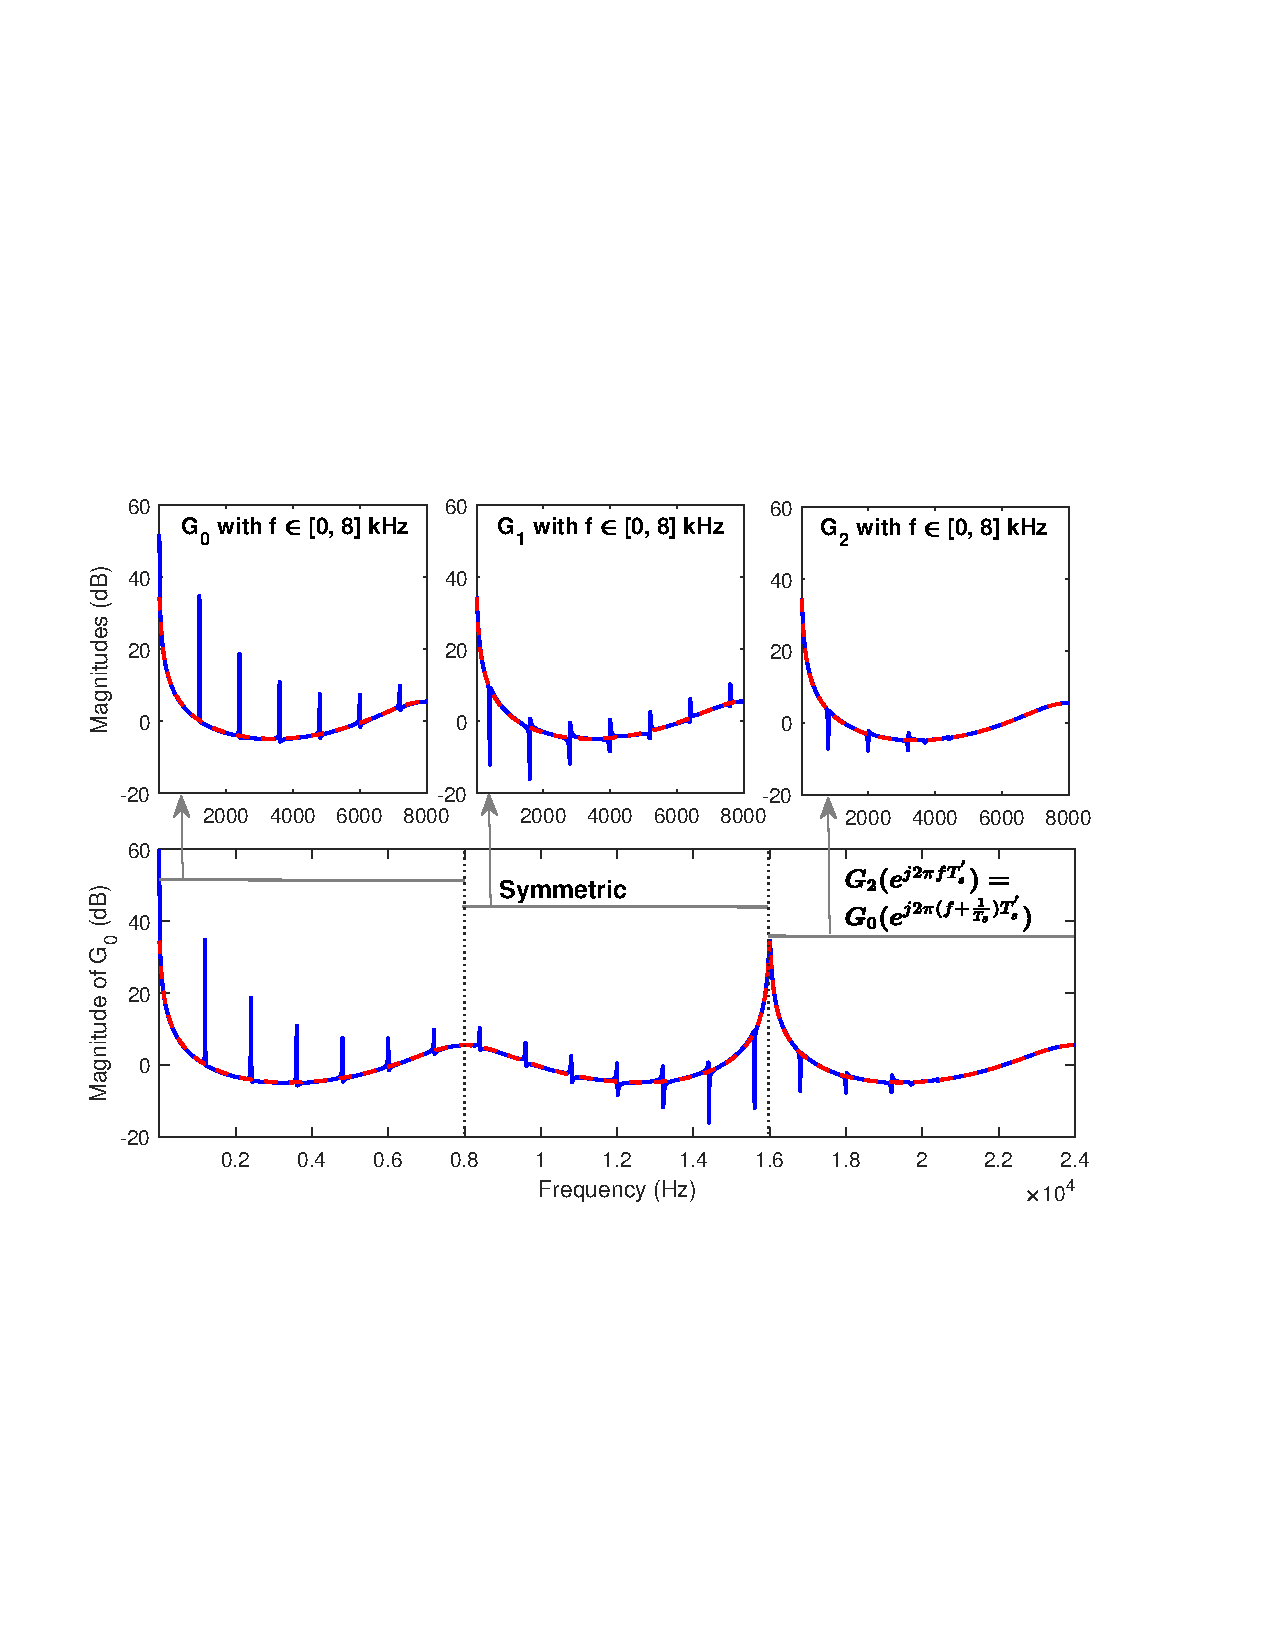
\includegraphics[width=13cm]{Fractional-order-RC/G_all}
\par\end{centering}
\caption{\label{fig:The-relationship-between}The relationships between $G_{0}(\text{e}^{j2\pi fT_{s}^{'}})$,
$G_{1}(\text{e}^{j2\pi fT_{s}^{'}})$, and $G_{2}(\text{e}^{j2\pi fT_{s}^{'}})$.}
\end{figure}
 

It will be shown next that the undesired magnitude characteristics
of $G_{0}(\text{e}^{j2\pi fT_{s}^{'}})$ arise from an implicit model
mismatch. Recall that
\begin{equation}
G_{0}(\text{e}^{j2\pi fT_{s}^{'}})=1+P(\text{e}^{j2\pi fT_{s}})C_{all}(\text{e}^{j2\text{\ensuremath{\pi}}fT_{s}^{'}}).\label{eq:G_0}
\end{equation}

Substituting (\ref{eq:C-all-fre}) into (\ref{eq:G_0}) gives
\begin{equation}
\begin{array}{c}
G_{0}(\text{e}^{j\Omega T_{s}^{'}})=\frac{[P(\text{e}^{j\Omega T_{s}})\hat{P}^{-1}(\text{e}^{j\Omega T_{s}^{'}})-1]\text{e}^{-jm\Omega T_{s}^{'}}Q(\text{e}^{j\Omega T_{s}^{'}})}{1-\text{e}^{-jm\Omega T_{s}^{'}}Q(\text{e}^{j\Omega T_{s}^{'}})}\\
+\frac{1+P(\text{e}^{j\Omega T_{s}})C_{dh}(\text{e}^{j\Omega T_{s}^{'}})}{1-\text{e}^{-jm\Omega T_{s}^{'}}Q(\text{e}^{j\Omega T_{s}^{'}})}.
\end{array}\label{eq:G_0-1}
\end{equation}

\begin{figure}[!ht]
\begin{centering}
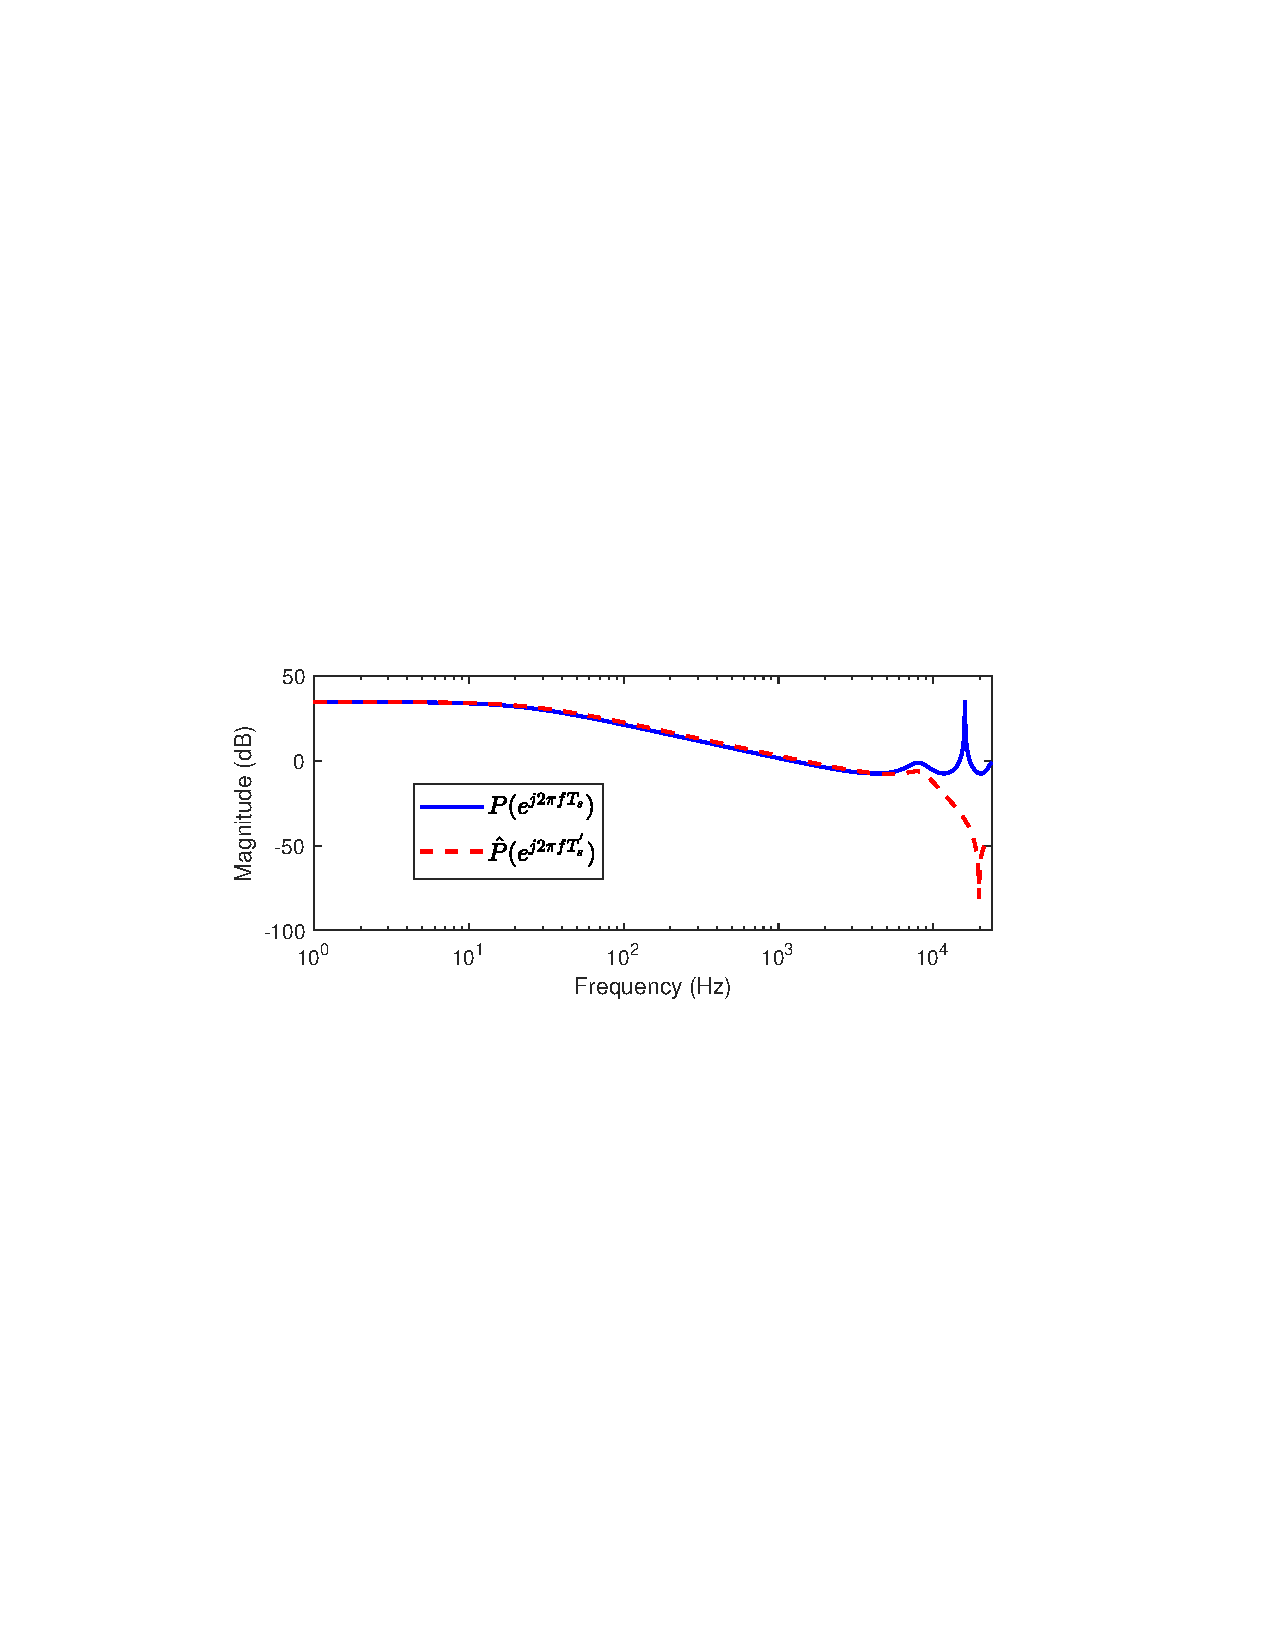
\includegraphics[width=11cm]{Fractional-order-RC/P_Ts_P_Ts_prime}
\par\end{centering}
\caption{\label{fig:The-relationship-between-1}Magnitude responses of $P(\text{e}^{j\Omega T_{s}})$
and $\hat{P}(\text{e}^{j\Omega T_{s}^{'}})$ .}
\end{figure}
Fig. \ref{fig:The-relationship-between-1} presents the frequency
responses of $P(\text{e}^{j\Omega T_{s}})$ and $\hat{P}(\text{e}^{j\Omega T_{s}^{'}}).$
At low frequencies, $P(\text{e}^{j\Omega T_{s}})\thickapprox P(\text{e}^{j\Omega T_{s}^{'}})\thickapprox\hat{P}(\text{e}^{j\Omega T_{s}^{'}})$,
and (\ref{eq:G_0-1}) reduces to
\begin{equation}
G_{0}(\text{e}^{j\Omega T_{s}^{'}})=\frac{1+P(\text{e}^{j\Omega T_{s}})C_{dh}(\text{e}^{j\Omega T_{s}^{'}})}{1-\text{e}^{-jm\Omega T_{s}^{'}}Q(\text{e}^{j\Omega T_{s}^{'}})}.\label{eq:G_0_low}
\end{equation}

$G_{0}(\text{e}^{j\Omega T_{s}^{'}})$ thus generates high gains where
the magnitude responses of the denominator $1-z^{-m}Q(z)$ are designed
to be small (Fig. \ref{fig:Q_multirate}). At high frequencies, intrinsic
model mismatches exist between $P(\text{e}^{j\Omega T_{s}})$ and
$\hat{P}(\text{e}^{j\Omega T_{s}^{'}})$ due to different sampling
frequencies. Even though the magnitude response of $\left.1-\text{e}^{-jm\omega}Q(\text{e}^{j\omega})\right|_{\omega=\Omega T_{s}^{'}}$
is small, the first term of (\ref{eq:G_0-1}) must be carefully considered.
To eliminate the undesired magnitude shapes, $Q(\text{e}^{j\Omega T_{s}^{'}})$
should be designed small enough at high frequencies to reduce the
effect of the model mismatches in $[P(\text{e}^{j\Omega T_{s}})\hat{P}^{-1}(\text{e}^{j\Omega T_{s}^{'}})-1]\text{e}^{-jm\Omega T_{s}^{'}}Q(\text{e}^{j\Omega T_{s}^{'}})$.
\begin{figure}[!ht]
\begin{centering}
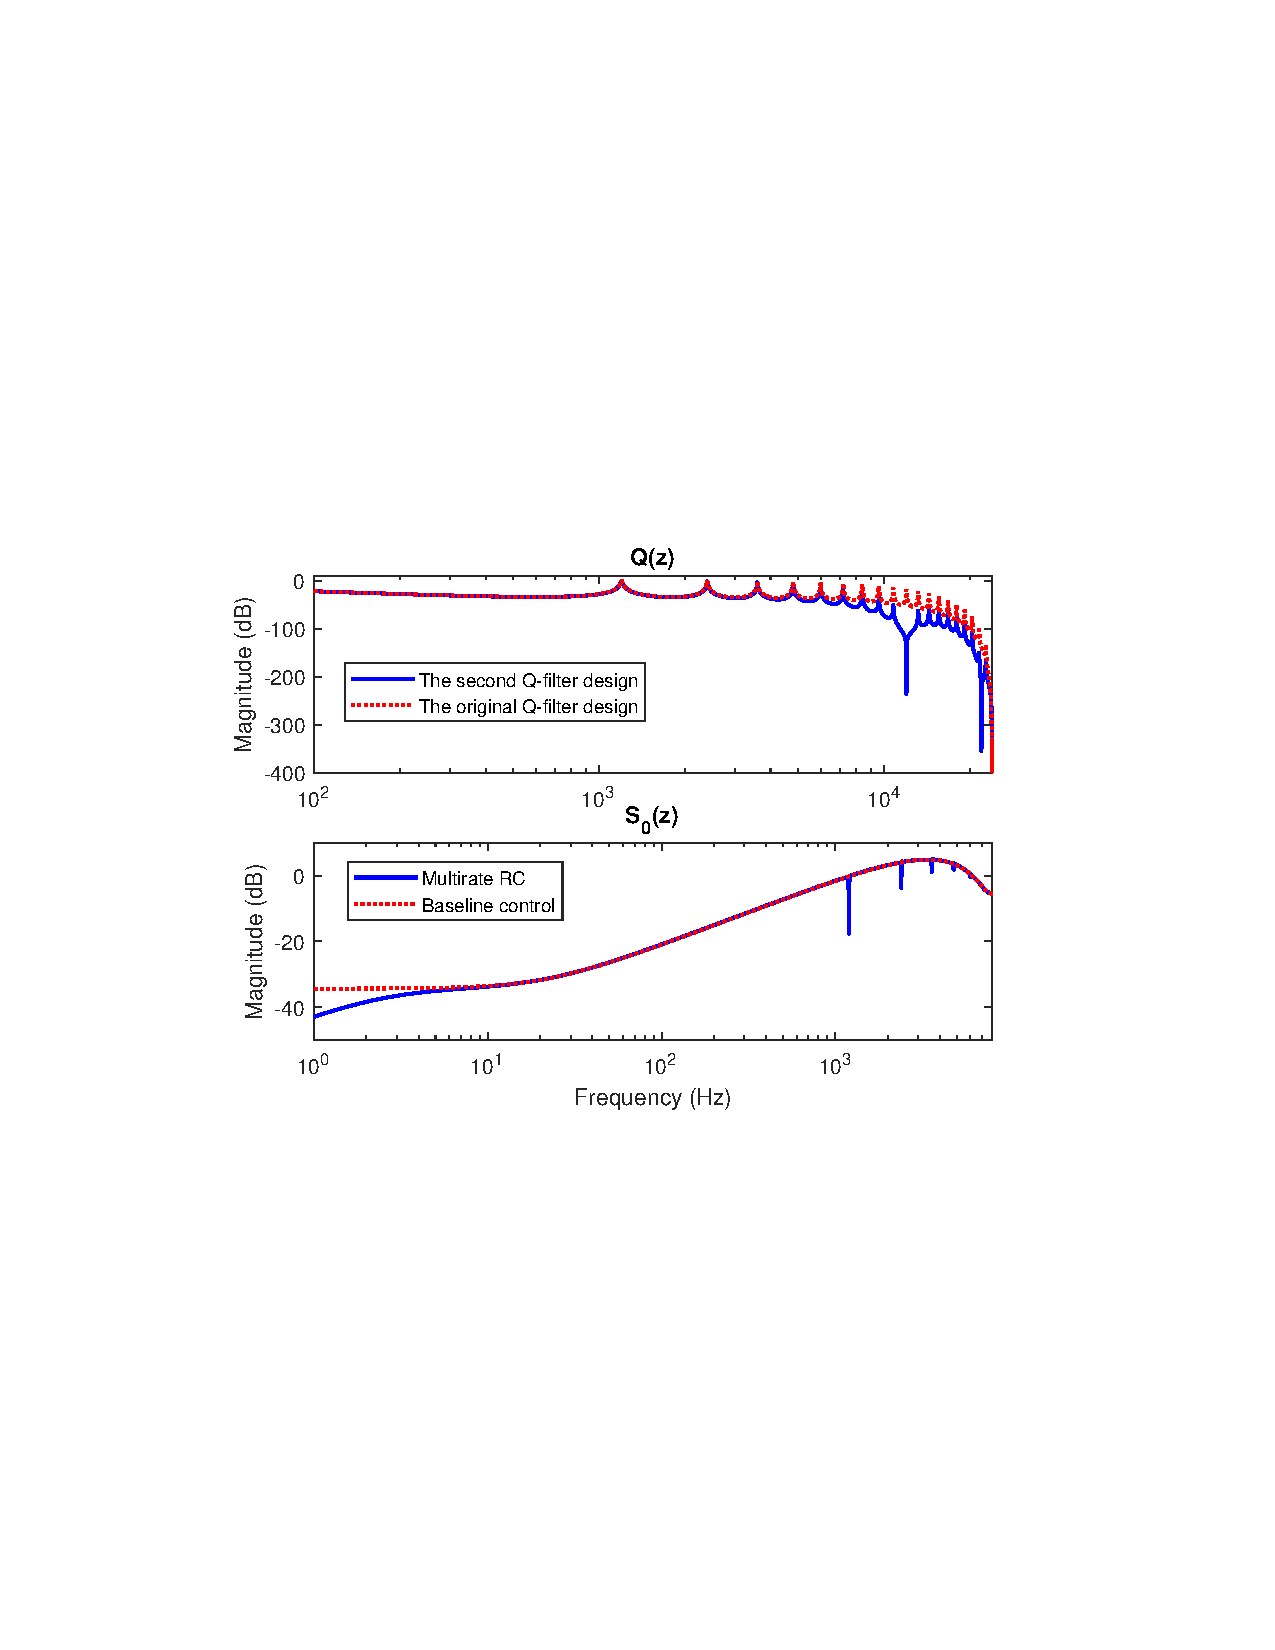
\includegraphics[width=10cm]{Fractional-order-RC/Q_S_another_Q}
\par\end{centering}
\caption{\label{fig:Magnitude-responses-of}Magnitude responses of the second
$Q$-filter design.}
\end{figure}

Compared with the original $Q$-filter design used in Fig. \ref{fig:Sensitivity_func},
the multirate RC thus demands an enhanced design with reduced $Q(\text{e}^{j\Omega T_{s}^{'}})$
at high frequencies (the top plot in Fig. \ref{fig:Magnitude-responses-of}).
This second $Q$-filter is designed with $\alpha=0.999$, $n_{0}=2$,
$\Omega_{1}=2\pi\times(12\,\text{kHz})$, and $\Omega_{2}=2\pi\times(22\,\text{kHz})$
(see Section \ref{sec:Repetitve-Control}). As a result, in the multirate
RC using the second $Q$-filter design, the undesired selective small
gains of $|G_{0}(\text{e}^{j2\pi fT_{s}^{'}})|$ disappear (the bottom
plot of Fig. \ref{fig:The-relationship-between-2}), which yields
a clear magnitude response of the closed-loop sensitivity function
with no visible error amplifications, as shown in the bottom plot
in Fig. \ref{fig:Magnitude-responses-of}.
\begin{figure}[!ht]
\begin{centering}
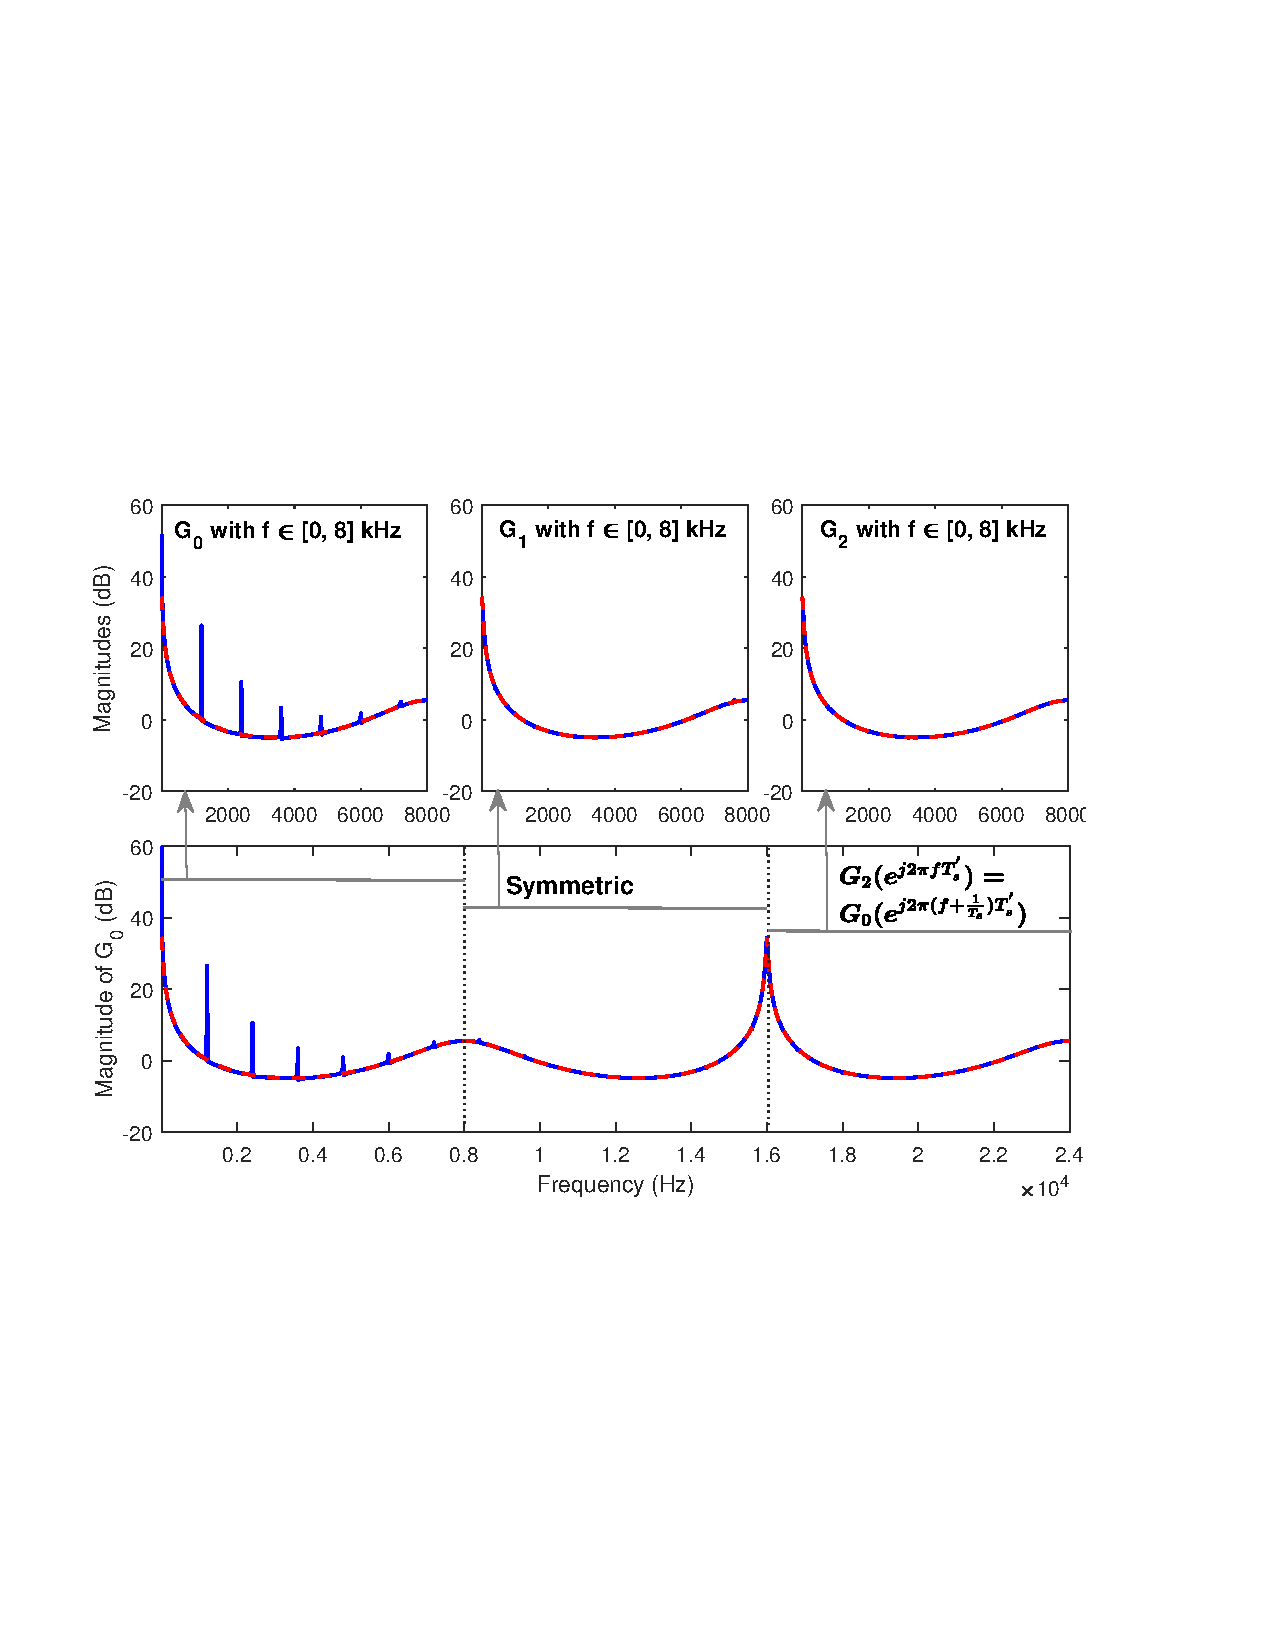
\includegraphics[width=13cm]{Fractional-order-RC/G_all_another_Q}
\par\end{centering}
\caption{\label{fig:The-relationship-between-2}$G_{0}(\text{e}^{j2\pi fT_{s}^{'}})$,
$G_{1}(\text{e}^{j2\pi fT_{s}^{'}})$, and $G_{2}(\text{e}^{j2\pi fT_{s}^{'}})$
of the second $Q$-filter design.}
\end{figure}

For more general cases in the multirate RC, the analysis steps are:
\begin{enumerate}
\item Given $f_{s}$ and $f_{0}$, identify the second sampling frequency
$f_{s}^{'}=\text{LCM}(f_{s},\,f_{0})$ for multirate RC design. Let
$F=T_{s}/T_{s}^{'}=f_{s}^{'}/f_{s}$.
\item Design the repetitive controller in (\ref{eq:C-all-fre}) under the
deviated sampling frequency to get desired disturbance-attenuation
properties.
\item Calculate and plot the closed-loop sensitivity function $S_{0}(\text{e}^{j\Omega T_{s}})$
and $G(\text{e}^{j\Omega T_{s}})$ in (\ref{eq:S}) to check if undesired
selective small gains show up.
\item Look into $G_{k}(\text{e}^{j2\pi fT_{s}^{'}})$ ($k=0,\,1,\,2,\,\cdots,\,F-1$)
with $f\in[0,\,f_{s}/2]$ to disentangle $G(\text{e}^{j\Omega T_{s}})$
in the summation form. Since all $G_{k}(\text{e}^{j2\pi fT_{s}^{'}})$'s
map into $G_{0}(\text{e}^{j2\pi fT_{s}^{'}})$, it suffices to analyze
$G_{0}(\text{e}^{j2\pi fT_{s}^{'}})$ under $f\in[0,\,f_{s}^{'}/2]$
to identify the frequencies of the undesired notches.
\item Redesign the $Q$-filter in the repetitive controller, and repeat
steps 2–4 to reduce the undesired selective small gains until the
design requirements are satisfied. 
\end{enumerate}

\subsubsection{Stability and Robustness} \label{sssec:Stability-and-robustness}

For stability and robustness analysis, the second condition in Theorem \ref{thm:small-gain-theorem} in Section \ref{subsec:Stability-and-Robustness} translates to $|\Delta(e^{j\Omega T_{s}})|<1/|T(e^{j\Omega T_{s}})|$, where $T(z)=\frac{P(z)C(z)}{1+P(z)C(z)}$ is the complementary sensitivity
function.

\begin{figure}[!ht]
\begin{centering}
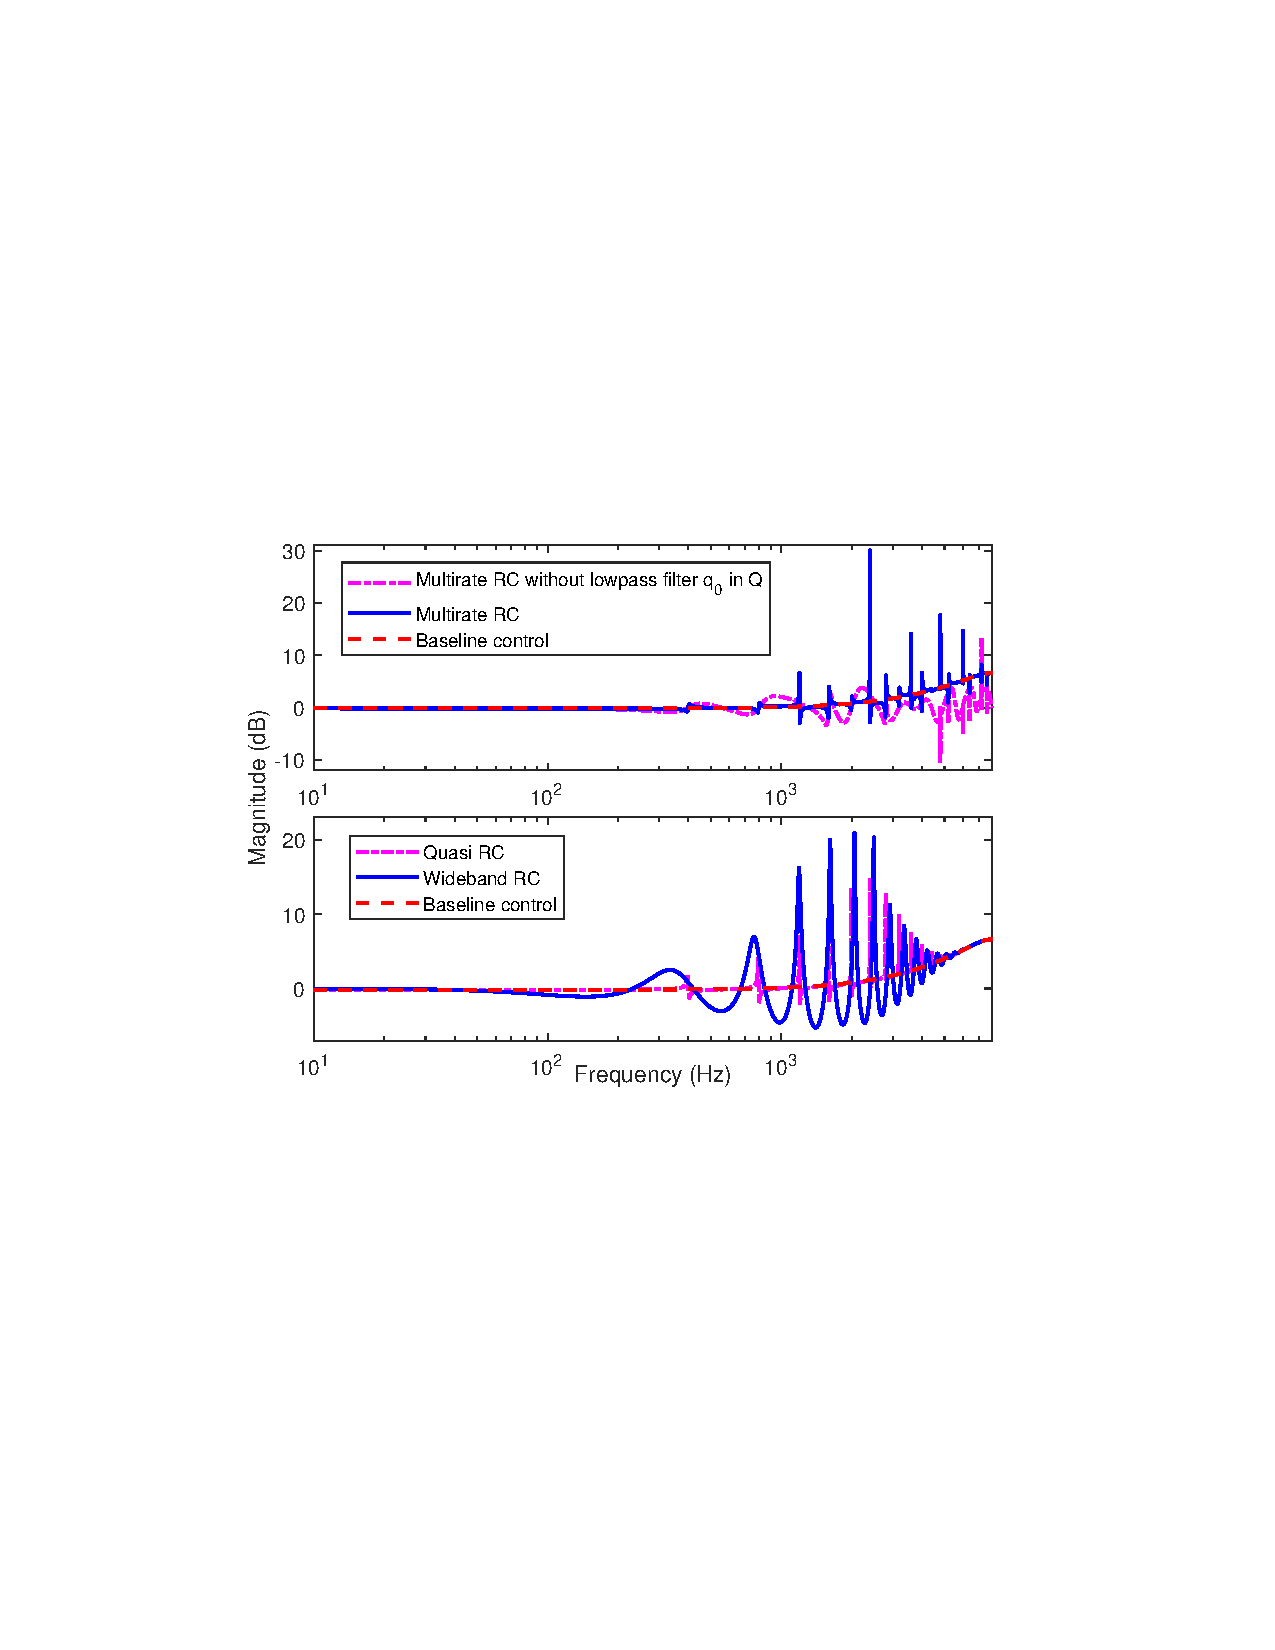
\includegraphics[width=11cm]{Fractional-order-RC/stability_all}
\par\end{centering}
\caption{\label{fig:invT-multirate-RC}Magnitude responses of $1/T(z)$, which
specify the upper bounds of the plant uncertainties to keep robustness.}
\end{figure}

Thus, $1/|T(e^{j\Omega T_{s}})|$ specifies the upper bound of the
plant uncertainty at all frequencies. Fig. \ref{fig:invT-multirate-RC}
shows the magnitude responses of $1/T(z)$ from the example in Section
\ref{sec:Verification-Galvo-Scanner}. Compared with the baseline control
(PID control in this example), the introduction of the multirate RC
extensively preserves and increases the robust stability bounds, especially
at high frequencies. With the multirate RC (solid line in the top
plot of Fig. \ref{fig:invT-multirate-RC}), the minimal $1/|T(e^{j\Omega T_{s}})|$
is $-2.9$ dB at 1203 Hz, which requires the magnitude response of
the uncertainty not to be greater than 71.6\% of the magnitude response
of the plant at this frequency. Without the lowpass filter $q_{0}(z^{-1})q_{0}(z)$
(dash-dot line in the top plot), the minimal $1/|T(e^{j\Omega T_{s}})|$
of the multirate RC decreases to $-10.6$ dB (29.5\%) at 4801 Hz.
Thus, the lowpass filter improves the robustness of the multirate
repetitive controller.

The minimal $1/|T(e^{j\Omega T_{s}})|$ of the wide-band RC (solid
line in the bottom plot) is $-5.25$ dB at 1404 Hz, that is, the uncertainty
magnitude at this frequency should be less than 54.6\% of the frequency
response of the plant. In the quasi RC (dash-dot line in the bottom
plot), the upper bound of the plant uncertainties is -2.16 dB (78\%)
(located at 1203 Hz). The quasi RC is more robust than the wide-band
RC, although as shall be discussed in the next section, these two
RCs have similar disturbance-attenuation performances. 

\section{Numerical and Experimental Verification in a Dual-axis Galvo Scanner} \label{sec:Verification-Galvo-Scanner}

This section provides implementation guidance and performance comparison
of the theoretical analyses. As a case study, the proposed fractional-order
RC algorithms are employed to reduce the crosstalk in the collaborative
control of the galvo scanner (see Section \ref{subsec:Collaborative-control-galvo-scanner}).

To attenuate crosstalk-induced disturbances with fractional-order
periods in the X channel, the wide-band, quasi, and multirate RC designs
in Section \ref{sec:Proposed-Fractional-order-RC} are implemented on top of the baseline
X-channel controller.

The identified plant model with the sampling time $T_{s}^{'}=1/48\,\text{ms}$
is
\begin{equation}
P^{'}(z)=\frac{0.061z^{2}+0.103z+0.061}{z^{5}-1.485z^{4}+1.032z^{3}-0.433z^{2}-0.057z-0.061}.\label{eq:P_z}
\end{equation}

A stable plant model under the sampling time $T_{s}=1/16\,\text{ms}$
is:
\begin{equation}
P(z)=\frac{0.061z^{4}+0.737z^{3}+0.351z^{2}+0.034z+0.0001}{z^{5}+0.144z^{4}-0.773z^{3}-0.359z^{2}-0.034z-0.0001}.\label{eq:P_z-1}
\end{equation}

Fig. \ref{fig:Bode-plot-of} shows the frequency responses of the
measured and identified $P^{'}(z)$ of the X channel in (\ref{eq:P_z}).
\begin{figure}[!ht]
\begin{centering}
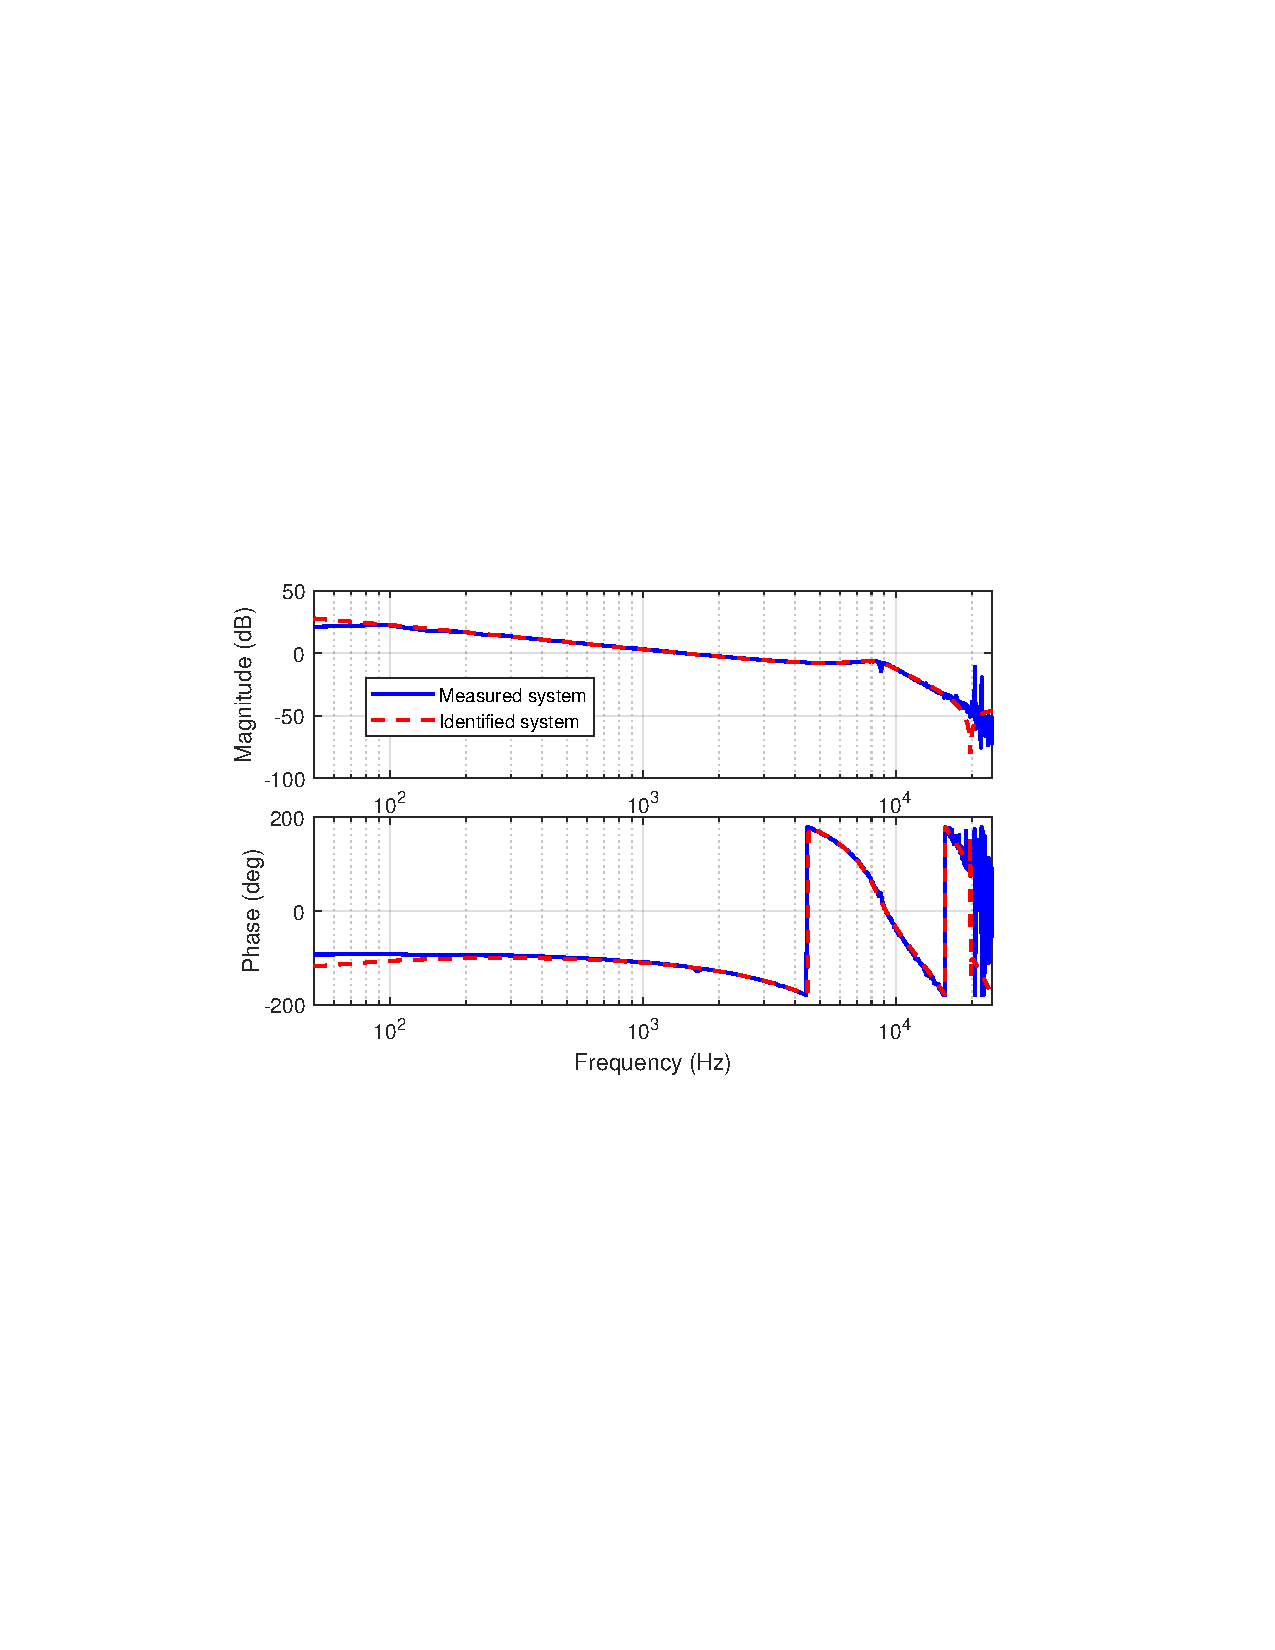
\includegraphics{Fractional-order-RC/bode_plant}
\par\end{centering}
\caption{\label{fig:Bode-plot-of}Bode plot of $P^{'}(z)$ sampled at $T_{s}^{'}$.}
\end{figure}

The plant models already contain a factory built-in PID-type controller.
The baseline feedback loop (Fig. \ref{fig:Block-diagram-RC} without
the plug-in compensator) is thus designed under the sampling time
of $T_{s}=1/16\,\text{ms}$ by applying $P(z)$ in (\ref{eq:P_z-1})
and by letting $C(z)=1$ (see Section \ref{sec:Proposed0-controller-factorization} or \cite{wang2017tutorial}). Such a design
provides a $4400\,\text{Hz}$ bandwidth in the complementary sensitivity
function $T(z)$. Throughout Sections \ref{subsec:Numerical-Verification-Galvo-Scanner}
and \ref{subsec:Experimental-Verification-Galvo-Scanner}, $n_{0}$ in (\ref{eq:q-1})
is chosen to be 3, and $M$ in (\ref{eq:Qz_q0}) equals zero.

\subsection{Numerical Verification} \label{subsec:Numerical-Verification-Galvo-Scanner}

In numerical verification, the same periodic disturbance with five
frequency components is introduced into the X-channel loop (Figs.
\ref{fig:Block-diagram-RC} and \ref{fig:Block-diagram-RC-1}): $d(k)=A\sum_{n=1}^{5}\sin(2\pi nf_{0}T_{s}k)$
with $A=4\,\text{mV}$ (corresponding to $0.006^{\circ}$ of the Y-channel
mirror rotation) and $f_{0}=1200\,\text{Hz}$. As shown in Fig. \ref{fig:Schematic-diagram-of},
the position mismatch of the laser hitting the powder bed is $L\tan2\theta=1\text{m}\times\tan(2\times0.006^{\circ})\approx0.21\,\text{mm}$.
When the length of the track to be sintered is 1 mm, this mismatch
causes an error of 21\%. 
\begin{figure}[!ht]
\begin{centering}
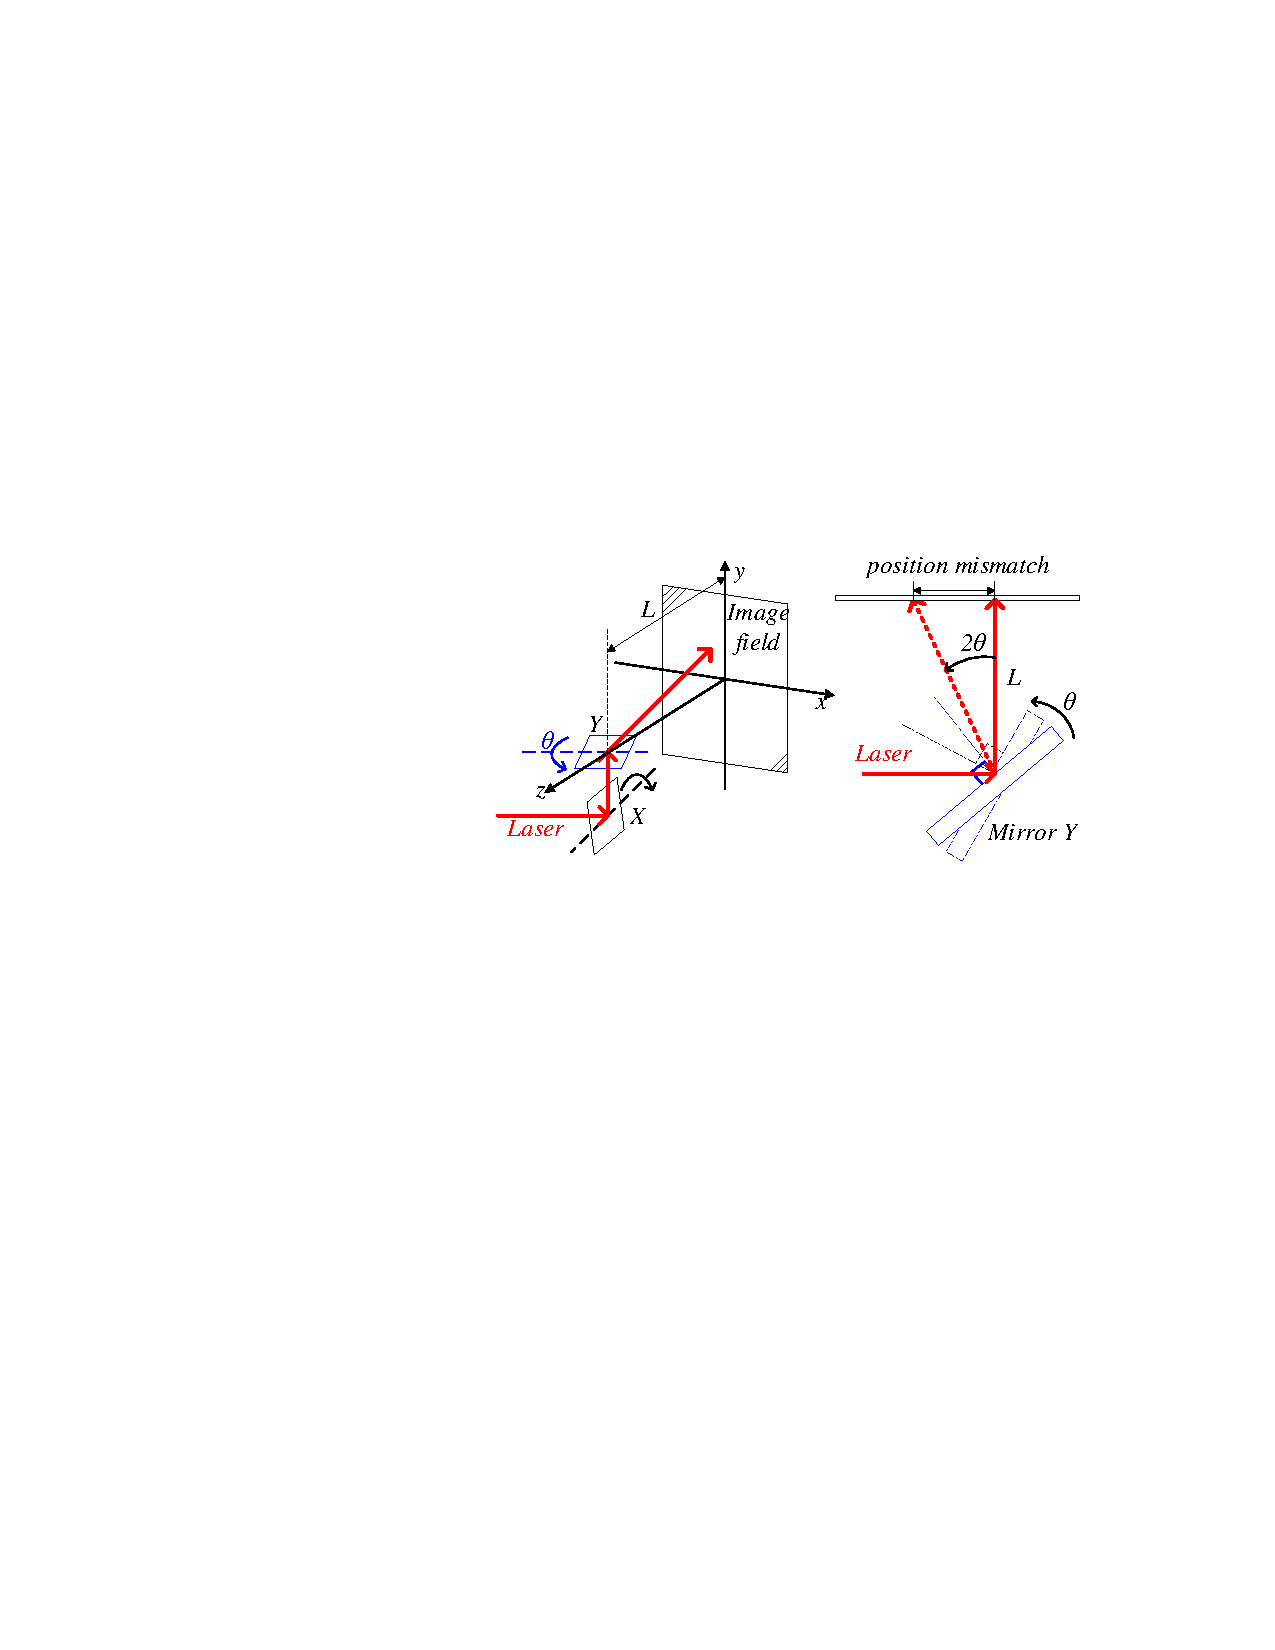
\includegraphics[width=10cm]{Fractional-order-RC/laser scanning mirror rotation}
\par\end{centering}
\caption{\label{fig:Schematic-diagram-of}Schematic diagram of galvo scanner
and position mismatch.}
\end{figure}
The dotted line in Fig. \ref{fig:Yd(t)_wideband-multirate} presents
the output of the baseline feedback loop in the time domain. Since
the PID controller is generic and not tailored to the repetitive disturbance,
the baseline controller barely attenuates the frequency spike at $1200\,\text{Hz}$
and provides limited attenuation to the other four spikes (the top
plot of Fig. \ref{fig:FFT}).
\begin{figure}[!ht]
\begin{centering}
\includegraphics[width=12cm]{Fractional-order-RC/wideband_baseline_multirate_time}
\par\end{centering}
\caption{\label{fig:Yd(t)_wideband-multirate}Plant outputs under baseline
control, and the proposed wide-band RC and multirate RC.}
\end{figure}
The wide-band and quasi RC algorithms are both implemented at the
sampling time of $T_{s}=1/16\,\text{ms}$, i.e. $f_{s}=16\,\text{kHz}$.
The relative degree of $P(z)$ in (\ref{eq:P_z-1}) is 1, that is,
$m=1$. In the wide-band RC, $N=\text{round}(f_{s}/f_{0})=\text{round}(16000/1200)=13$.
Under this configuration, the frequency spikes the plug-in compensator
targets are at $f_{s}/N=1230.77\,\text{Hz}$ and its integer multiples.
A wider attenuation width is needed in $1-z^{-m}Q(z)$ to cover the
adjacent harmonics at $1200\,\text{Hz}$, $2400\,\text{Hz}$, $3600\,\text{Hz}$,
etc. To achieve this goal, $\alpha$ is set as 0.8, as shown in Fig.
\ref{fig:Q_wideband}.
\begin{figure}[!ht]
\begin{centering}
\includegraphics[width=11cm]{Fractional-order-RC/Spectrum_all}
\par\end{centering}
\caption{\label{fig:FFT}FFT of plant output sampled at $T_{s}$.}
\end{figure}
In the quasi RC, the fictitious fundamental frequency is configured
at $400\,\text{Hz}$ such that $N=16000/400=40$. Thus, the plug-in
compensator generates high gains at $400\,\text{Hz}$ and its integer
multiples, covering the target frequencies $\{1200i\,\text{Hz}\}\,(i\in\mathbb{Z}^{+})$.
$\alpha$ is designed to be $0.999$ to achieve good steady-state
performance. The time-domain result of the quasi RC is similar to
the wide-band RC result shown in the dash-dotted line in Fig. \ref{fig:Yd(t)_wideband-multirate}
and is omitted here. The time-domain outputs show that the wide-band
and quasi RCs work better than the baseline control. The frequency-domain
analysis in Fig. \ref{fig:FFT} further shows the first two frequency
spikes are remarkably reduced compared with the baseline control.
Due to the decreased control effort, the high-frequency spikes at
$3600\,\text{Hz}$, $4800\,\text{Hz}$, and $6000\,\text{Hz}$ remain
largely unchanged. 

In the multirate RC, the plug-in compensator is designed at $T_{s}^{'}=1/48\,\text{ms}$
($f_{s}^{'}=48\,\text{kHz}$) with $F=T_{s}/T_{s}^{'}=3$. The relative
degree of $P^{'}(z)$ in (\ref{eq:P_z}) is 3 ($m=3$). $\alpha$
is chosen to be 0.999 to reduce the waterbed effect. In this case,
$N=f_{s}^{'}/f_{0}=48000/1200=40$. In Fig. \ref{fig:Q_multirate},
small gains of $1-z^{-m}Q(z)$ are generated exactly at $1200\,\text{Hz}$
and its integer multiples. The increased control efforts at high frequencies
yield a further-attenuated output in the time domain (the solid line
in Fig. \ref{fig:Yd(t)_wideband-multirate}) and in the frequency
domain (the bottom plot of Fig. \ref{fig:FFT}). Besides the attenuated
low-frequency spikes, the peaks at $3600\,\text{Hz}$, $4800\,\text{Hz}$,
and $6000\,\text{Hz}$ are also largely reduced.

The numerical results of the four control systems are compared in
Table \ref{tab:Experimental-results-of}. As a performance metric,
for each control system, the $3\sigma$ value of the time-domain result
is provided, where $\sigma$ denotes the standard deviation. Compared
with the baseline control, the application of the multirate, wide-band,
and quasi RC algorithms decreases the $3\sigma$ values, thereby achieving
the desired disturbance-attenuation effect. In more details, the wide-band
and quasi RCs have similar performance, and the performance gains
are $35\%$ and $34\%$, respectively. The multirate RC outperforms
the other two by reaching a $64\%$ decrease of the $3\sigma$ value
and reducing the laser point mismatch by one order of magnitude to
$0.21\times(1-64\%)\approx0.075\,\text{mm}$. In the case of a 1 mm
track, the sintering error reduces from 21\% to 7\%.
\begin{table}[!ht]
\caption{\label{tab:Experimental-results-of}Numerical and experimental results
of the baseline control and the three proposed RC schemes. (N/A denotes
``not applicable.'')}
\begin{centering}
% \resizebox{\linewidth}{!}{%
\begin{tabular}{@{} cccccc @{}} 
\toprule
& & Baseline & Multirate & Wide-band & Quasi\\

\midrule
\multirow{2}{*}{Simulation} & 3$\sigma$ & 0.0147 & 0.0053 & 0.0096 & 0.0097 \\
& Decreasing & N/A & 64\% & 35\% & 34\% \\

\midrule
\multirow{2}{*}{Experiment} & 3$\sigma$ & 0.0132 & 0.0045 & 0.0074 & 0.0071 \\
& Decreasing & N/A & 66\% & 44\% & 46\% \\

\bottomrule
\end{tabular}
% }
\par\end{centering}
\end{table}

\subsection{Experimental Verification} \label{subsec:Experimental-Verification-Galvo-Scanner}

The control schemes are implemented on a dSPACE DS1104 processor board.
Without loss of generality, the Y channel is run with a simple harmonic
signal $A\sin(2\pi f_{0}t+\phi)$ with $A=8\,\text{V}$, $f_{0}=600\,\text{Hz}$,
and $\phi=0$. The periodic disturbance emerges on the output of the
X channel, with frequency spikes at $1200\,\text{Hz}$, $2400\,\text{Hz}$,
$3600\,\text{Hz}$, etc (the top plot in Fig. \ref{fig:FFT-exp}),
as stated in Section \ref{subsec:Collaborative-control-galvo-scanner}.
The baseline PID-type controller is unable to reduce the crosstalk
between the X and Y channels (the dotted line in Fig. \ref{fig:Yd(t)_wideband-exp}).
\begin{figure}[!ht]
\begin{centering}
\includegraphics[width=12cm]{Fractional-order-RC/Spectrum_all_exp}
\par\end{centering}
\caption{\label{fig:FFT-exp}FFT of plant output sampled at $T_{s}$.}
\end{figure}
\begin{figure}[!ht]
\begin{centering}
\includegraphics[width=12cm]{Fractional-order-RC/Wideband_multi_time_exp}
\par\end{centering}
\caption{\label{fig:Yd(t)_wideband-exp}Plant output of baseline control, and
the proposed wide-band RC and multirate RC.}
\end{figure}
The experimental and numerical results match well with each other.
The output signals $y_{d}(t)$ in Fig. \ref{fig:Yd(t)_wideband-exp}
show the clear performance difference of multirate RC$>$wide-band
RC($\approx$quasi RC)$>$baseline control. Indeed, frequency-domain
analysis reveals that the wide-band and quasi methods can reduce the
first two but not other high-frequency spikes above $3600\,\text{Hz}$.
The multi-rate RC algorithm, on the other hand, can effectively attenuate
the periodic frequency spikes appearing at $2nf_{0}$ ($n\in\mathbb{Z}^{+}$)
by generating frequency notches in $1-z^{-m}Q(z)$ and enhanced control
efforts exactly at those frequencies.

The slight differences between the simulated and experimental results
in Table \ref{tab:Experimental-results-of} are caused by the different
disturbance sources in the two cases. In simulations, the same amplitude
is selected for the five introduced frequency spikes. In experiments,
the disturbances induced by the crosstalk are different in amplitudes.
For each spike, as the frequency increases, the amplitude decreases
(Fig. \ref{fig:FFT-of-the}).

\section{Summary} \label{sec:Model-inverse-Summary}

In this chapter, three repetitive control (RC) algorithms are proposed
to overcome the intrinsic limitation of the RC internal model $1/(1-z^{-N})$
under fractional-order situations that arise in selective laser sintering
additive manufacturing. To apply repetitive error rejection when the
fundamental disturbance frequency does not divide the sampling frequency,
the wide-band RC scheme widens the attenuation widths to include the
desired frequencies of the periodic disturbance. The quasi RC method,
on the other hand, creates an integer $N$ by selecting the greatest
common divisor of the sampling and fundamental disturbance frequencies
as the fictitious fundamental frequency. The multirate RC applies
a new fast sampling frequency that allows for exact attenuation at
the desired repetitive frequencies. Numerical and experimental results
verify the effectiveness of all three algorithms, and the multirate
RC algorithm outperforms the wide-band and quasi ones by providing
more systematic, precise servo enhancement, particularly at high frequencies.

% ========== Chapter 8

\chapter{$H_\infty$-based Model Inversion} \label{chap:Model-Inversion}

\section{Introduction} \label{sec: Model-inversion-Introduction}

Given a linear time-invariant system model $G$, the inversion of
$G$ has numerous practical implementations including iterative learning
control (ILC) \cite{Bristow2006,shen2018iterative,de2019data}, repetitive
control \cite{wang2018multirate,zhu2017observer}, two-degree-of-freedom
servo in feedforward control \cite{Tomizuka1999,wang2016robust},
as well as Youla parameterization and disturbance observer in feedback
control \cite{jiang2019local,Ohnishi1993,chen2011minimum,apte2019disturbance,wang2017tutorial}.
Here, $G$ can be an open-loop plant model or a closed-loop control
system. For a minimum-phase system, $G^{-1}$ is stable and ready
to be implemented. However, for a system with nonminimum-phase (NMP
or unstable) zeros, $G^{-1}$ is unstable and cannot be implemented
directly. To find a stable, rational, and causal replacement $\hat{G}^{-1}$
such that $G\hat{G}^{-1}$ approximates 1 is thus a fundamental challenge
in inversion-based control designs. Such a challenge is more pronounced
in discrete-time systems since 1) integrator-type plant dynamics\footnote{When actuators take forces or torques as the input and linear/angular
position as the output, integrator-type plant dynamics with a relative
degree not less than two show up.}, common in motion control, generate NMP zeros in their zero-order-hold
(ZOH) equivalents when the sampling time is sufficiently small; 2)
fractional-order delays induce unstable zeros after discretization
\cite{Astrom1984_zerosOfSampledSys}.

Considering the importance and the challenge of model inversion,
numerous strategies have been established in modern literature. Based
on system representations and scopes of application, we can classify
these strategies into two categories: frequency- and time-domain model
inversions. The frequency-domain strategies focus on expressing the
transfer functions of the stable inverses and hence can be used in
both feedback and feedforward controls. Examples in this category
include the approximate (e.g., NPZ-ignore, ZPETC, and ZMETC) \cite{Tomizuka1987,dai2019quantitative,butterworth_analysis_2012,Butterworth2008},
the ILC-based \cite{devasia2017iterative,kim_modelingfree_2013,chen2016data},
and the $H_{\infty}$-based \cite{zheng2018systematic,francis_h_1984,zheng2017design}
model inversions. On the other hand, the time-domain strategies \cite{de2019finite,dewey1998experimental,Ramani:2017hx,van2018inversion}
aim at identifying the optimal control signal that minimizes the error
between a given reference and the output. These time-domain algorithms
are mainly used as feedforward techniques since a preview of the reference
is generally not available in feedback design.

This chapter studies the analysis and design of model inversion strategies
in the frequency domain. Current strategies in this category aim at
achieving effective model matching between $\hat{G}$ and $G$. Compared
with the approximate and the ILC-based model inversions, the $H_{\infty}$-based
model inversion can automatically identify the inverse model without
knowing the exact NMP zeros, which particularly benefits systems with
complicated pole-zero distributions. However, when the inverses are
to be implemented in feedback systems, additional considerations are
needed for assuring closed-loop stability and robustness. In pursuit
of bridging the gap between accurate model approximations and robust
feedback performances, this chapter builds a new $H_{\infty}$-based
optimal inversion algorithm that advances the field by 1) mitigating
control efforts at customized frequencies and thereby enhancing system
robustness; 2) reaching high efficiency for complex high-order systems
and unstable systems.

Before presenting the main algorithm, we first provide a pole-zero-map-based
NMP-zero modulation by replacing high-frequency NMP zeros with stable
ones in motion control applications. We verify the feasibility and
limit of this intuitive modulation in achieving a stable inverse model
and meanwhile capturing the low-frequency system dynamics for high-performance
motion control. Then we extend this intuitive modulation to an optimal
design of model inversion. There, replacing the manual adjustment
with an automatic and optimal search, we develop a new $H_{\infty}$-based
algorithm that can attain model accuracy at the frequency regions
of interest while constraining noise amplification elsewhere to guarantee
system robustness. The design goals are achieved by a multi-objective
formulation and an all-pass factorization that consider model matching,
gain constraints, causality of transfer functions, and factorization
of unstable system modes in a unified scheme. The proposed algorithm
is validated on motion control systems and complex high-order systems.
Moreover, along the path, we unveil previously ignored features of
existing inversion strategies by developing a general frequency-domain
analysis method, which also gives new insights into comparing the
performances of different strategies.

The main contributions of this chapter are:
\begin{enumerate}
\item conducting an up-to-date review of model inversion strategies and
proposing a new frequency-domain analysis method;
\item analyzing the effect of an intuitive NMP-zero modulation and developing
a new $H_{\infty}$-based inversion algorithm;
\item validating the proposed algorithm by presenting detailed case studies
with high-fidelity experimental data.
\end{enumerate}
The remainder of this chapter is structured as follows. Section \ref{sec:Review-of-Relevant}
conducts an in-depth review of literature and proposes the new frequency-domain
analysis method. Section \ref{sec:NMP-zero-Modulation} elucidates
the effect of modulating NMP zeros. The proposed optimal inversion
is presented and verified in Section \ref{sec:-based-Optimal-Design}.

\section{Review and comparison of frequency-domain inversion algorithms} \label{sec:Review-of-Relevant}

The frequency-domain inversion algorithms aim at expressing the stable
inverse models $F=\hat{G}^{-1}$ in the $s$- or $z$-domain. $\hat{G}$ is the minimum-phase system model that approximates
$G$ and has a stable inverse. An optimal inverse model is desired
for $G\hat{G}^{-1}$ to approximate 1. In this section, we review
and compare three typical types of frequency-domain inversion algorithms.
In addition, we unveil new features of existing algorithms by developing
a general frequency-domain analysis method.

\subsection{$H_{\infty}$-based Model Inversion} \label{subsec:-based-model-inversion}

\noindent \emph{1) Algorithm}

The model inversion problem for NMP systems has been solved using
the $H_{\infty}$ formulation \cite{francis_h_1984,zheng2017design,zheng2018systematic}.
For a continuous-time NMP system $G(s)=(b-s)/(b+s)$ with $b>0$,
under a cost function $J=||W(s)(1-G(s)\hat{G}^{-1}(s))||_{\infty}$,
where the weighting $W(s)=(k+\xi s)/(k+s)$ is a low-pass filter with
$k>0$ and $0\leq\xi<1$, the optimal inverse of $G(s)$ that minimizes
$J$ is a lead filter \cite{francis_h_1984}:
\begin{equation}
\hat{G}^{-1}(s)=\frac{k(1-\xi)(b+s)}{(k+b)(k+\xi s)}\label{eq:output_stable-1}
\end{equation}
that has high gains at high frequencies. The frequency response of
the optimal $G(s)\hat{G}^{-1}(s)$ is

\begin{equation}
G(j\Omega)\hat{G}^{-1}(j\Omega)=\frac{k(1-\xi)(b-j\Omega)}{(k+b)(k+j\xi\Omega)},\label{eq:GGhatinv}
\end{equation}

\noindent where $\Omega$ is in rad/s.

\

\noindent \emph{2) Frequency-domain Analysis}

To quickly capture the essence of $G\hat{G}^{-1}$, we examine the
frequency response of $G\hat{G}^{-1}$ at the two frequency endpoints
(0 and $\infty$ for a continuous-time system or 0 and $\pi$ in rad
for a discrete-time system) and evaluate the characteristics of model
matching.

Considering $b=2$, $\xi=0.3$, and different $k$'s, we depict in
Fig. \ref{fig:Nominal-model-inversion-2} the frequency responses
of (\ref{eq:GGhatinv}). 
\begin{figure}[!ht]
\begin{centering}
\includegraphics[width=10cm]{Model-inversion/Hinf}
\par\end{centering}
\caption{\label{fig:Nominal-model-inversion-2}Frequency responses of $G(j\Omega)\hat{G}^{-1}(j\Omega)$
with $b=2$, $\xi=0.3$, and different values of $k$}
\end{figure}
As $\Omega$ increases from 0 to $\infty$, the phase of $G(j\Omega)\hat{G}^{-1}(j\Omega)$
always goes from $0$ to $-180^{\circ}$ (the bottom plot of Fig.
\ref{fig:Nominal-model-inversion-2}), and its magnitude goes from
$b\left(\frac{1-\xi}{k+b}\right)$(<0 dB) to $\frac{k}{\xi}\left(\frac{1-\xi}{k+b}\right)$,
monotonically. Therefore, depending on the values of $k$ and $\xi$,
$G(s)\hat{G}^{-1}(s)$ is a high-pass filter when $\frac{k}{\xi}\left(\frac{1-\xi}{k+b}\right)>b\left(\frac{1-\xi}{k+b}\right)$,
i.e., $k>\xi b$ (0.6 in this example), a low-pass filter when $k<\xi b$,
and has a constant magnitude when $k=\xi b$ (the top plot of Fig.
\ref{fig:Nominal-model-inversion-2}).

\subsection{\label{subsec:Approximate-model-inversions}Approximate Model Inversions}

\noindent \emph{1) Algorithms}

For discrete-time NMP systems, to obtain the basic structure of the
inverse model, approximate model inversions \cite{butterworth_analysis_2012,dai2019quantitative,Butterworth2008,Tomizuka1987}
first factor out the unstable zeros of the system as
\begin{equation}
G(z)=\frac{N(z)}{D(z)}=\frac{N_{s}(z)N_{u}(z)}{D(z)},\label{eq:P_N_D}
\end{equation}
where $N(z)$ and $D(z)$ are coprime polynomials of $z$, and $N_{s}(z)$
and $N_{u}(z)$ contain, respectively, the stable and the unstable
zeros. Here, we define $N_{u}(z)$ as
\begin{align}
N_{u}(z) & =(z-z_{1})(z-z_{2})\cdots(z-z_{n}),\label{eq:N_zeros}
\end{align}
where $z_{1},\,z_{2},\,\cdots,\,z_{n}$ are outside the unit circle.
Note that
\begin{align*}
N_{u}(z^{-1}) & =(z^{-1}-z_{1})(z^{-1}-z_{2})\cdots(z^{-1}-z_{n})
\end{align*}
has stable zeros. In addition, $N_{u}(z)N_{u}(z^{-1})$ is zero-phase.

In the general case, the approximate inverse model of $G(z)$ in (\ref{eq:P_N_D})
has a structure of

\begin{equation}
\hat{G}^{-1}(z)=\frac{D(z)}{N_{s}(z)\tilde{N_{u}}(z)},\label{eq:G_hat_inv}
\end{equation}

\noindent where $\tilde{N_{u}}(z)$ is a design parameter.

Table \ref{tab:-in-approximate} summarizes three approximate model
inversions with different designs of $\tilde{N_{u}}(z)$. 
\begin{table*}
\caption{\label{tab:-in-approximate}$\tilde{N_{u}}(z)$, $G(z)\hat{G}^{-1}(z)$,
and $\frac{Y(z)}{R(z)}$ in approximate model inversions. $Y(z)$
and $R(z)$ are transfer functions of the output and reference signals
shown in Fig. \ref{fig:Block-diagram-for-1}.}

\centering{}{\setlength{\extrarowheight}{4pt}%
\begin{tabular*}{12cm}{@{\extracolsep{\fill}}c|ccc}
\hline 
Methods & NPZ-ignore & ZPETC & ZMETC\tabularnewline
\hline 
$\tilde{N_{u}}(z)$ & $N_{u}(1)$ & $\frac{[N_{u}(1)]^{2}}{N_{u}(z^{-1})}$ & $N_{u}(z^{-1})$\tabularnewline
$G(z)\hat{G}^{-1}(z)$ & $\frac{N_{u}(z)}{N_{u}(1)}$ & $\frac{N_{u}(z)N_{u}(z^{-1})}{[N_{u}(1)]^{2}}$ & $\frac{N_{u}(z)}{N_{u}(z^{-1})}$\tabularnewline
$\frac{Y(z)}{R(z)}$ & $z^{-m}\frac{N_{u}(z)}{N_{u}(1)}$ & $z^{-m}\frac{N_{u}(z)N_{u}(z^{-1})}{[N_{u}(1)]^{2}}$ & $z^{-m}\frac{N_{u}(z)}{N_{u}(z^{-1})}$\tabularnewline
$\frac{Y(\text{e}^{j\omega})}{R(\text{e}^{j\omega})}$ & $\text{e}^{-jm\omega}\frac{N_{u}(\text{e}^{j\omega})}{N_{u}(1)}$ & $\text{e}^{-jm\omega}\frac{N_{u}(\text{e}^{j\omega})N_{u}(\text{e}^{-j\omega})}{[N_{u}(1)]^{2}}$ & $\text{e}^{-jm\omega}\frac{N_{u}(\text{e}^{j\omega})}{N_{u}(\text{e}^{-j\omega})}$\tabularnewline
$\left|\frac{Y(\text{e}^{j\pi})}{R(\text{e}^{j\pi})}\right|$ & $\left|\frac{N_{u}(-1)}{N_{u}(1)}\right|$ & $\left[\frac{N_{u}(-1)}{N_{u}(1)}\right]^{2}$ & 1\tabularnewline
\hline 
\end{tabular*}}
\end{table*}
The NMP zeros ignore method (NPZ-ignore) \cite{butterworth_analysis_2012,Butterworth2008}
replaces $N_{u}(z)$ with $\tilde{N_{u}}(z)=N_{u}(1)$ at the cost
of magnitude and phase mismatch in $G(z)\hat{G}^{-1}(z)$. The zero-phase-error-tracking
control (ZPETC) \cite{Tomizuka1987} assigns instead $\tilde{N_{u}}(z)=[N_{u}(1)]^{2}/N_{u}(z^{-1})$
and achieves zero-phase error dynamics since $G(z)\hat{G}^{-1}(z)=N_{u}(z)N_{u}(z^{-1})/[N_{u}(1)]^{2}$
is zero-phase. The zero-magnitude-error-tracking control (ZMETC) \cite{butterworth_analysis_2012},
on the other hand, eliminates all magnitude errors by converting the
unstable zeros to their stable reciprocals, namely, $\tilde{N_{u}}(z)=N_{u}(z^{-1})$.
Note that $N_{u}(1)$ in NPZ-ignore and $[N_{u}(1)]^{2}$ in ZPETC
are added to create a unity DC gain of $G(z)\hat{G}^{-1}(z)$.

Furthermore, to make the approximate inverse model $\hat{G}^{-1}(z)$
in (\ref{eq:G_hat_inv}) realizable and ready to be implemented as
a block during feedback/feedforward implementation, a causal inverse
model is obtained by multiplying $\hat{G}^{-1}(z)$ with $z^{-m}$:

\begin{equation}
F(z)=z^{-m}\hat{G}^{-1}(z)=z^{-m}\frac{D(z)}{N_{s}(z)\tilde{N_{u}}(z)},\label{eq:P_hat_inv}
\end{equation}
\begin{equation}
m=Order[Denominator\;of\;\hat{G}(z)]-Order[Numerator\;of\;\hat{G}(z)]\label{eq:relative_degree}
\end{equation}
is the relative degree of $\hat{G}(z)$ and the $Order$ function
calculates the highest exponent in a transfer function. Next we will
prove that $m$ is always larger than 0 in the NPZ-ignore, ZPETC,
and ZMETC.
\begin{proof}
We can tell from Table \ref{tab:-in-approximate} that the relative
degree of $\tilde{N_{u}}(z)$ is 0 in each of the three designs. Thus,
from (\ref{eq:G_hat_inv}), the expression of $m$ in (\ref{eq:relative_degree})
can be reduced to

\begin{equation}
m=Order[D(z)]-Order[N_{s}(z)].\label{eq:relative_deg_sim}
\end{equation}
Also, we have $Order[D(z)]\geq Order[N_{s}(z)]+Order[N_{u}(z)]$ from
(\ref{eq:P_N_D}) and $Order[N_{u}(z)]>0$ for NMP systems, yielding
$Order[D(z)]>Order[N_{s}(z)]$, that is, $m>0$ in (\ref{eq:relative_deg_sim}). 
\end{proof}
Here, the result $m>0$ means the delay $z^{-m}$ should always be
accounted for to make the inverse model realizable in the feedback/feedforward
applications of approximate model inversions. In feedforward applications
where a preview of the desire output $y_{d}(k)$ is available, the
delay $z^{-m}$ can be canceled out by letting $r(k)=y_{d}(k+m)$.

\

\noindent \emph{2) Frequency-domain Analysis}

Fig. \ref{fig:Block-diagram-for-1} shows a block diagram to illustrate
the goal of the model inversion design, where $r$, $u$, and $y$
represent the reference, the input, and the output signals, respectively.
Note that subsequently $F$ can be implemented as a block in the feedback/feedforward
controller designs, such as the examples in Section \ref{subsec:Feedback-applications-of}.
\begin{figure}[!ht]
\begin{centering}
% \resizebox{8.4cm}{!}{%
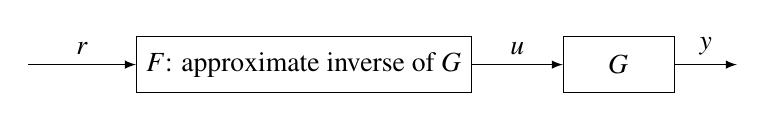
\begin{tikzpicture}[auto, node distance=4cm, >=latex] 

\node [input, name=input] {}; 
\node [block, right of=input, node distance=3.5cm] (controller) {$F$: approximate inverse of $G$};
\node [block, right of=controller] (plant) {$G$};
\node [output, right of=plant, node distance=1.5cm] (output) {};

\draw [->] (input) -- node {$r$} (controller);
\draw [->] (controller) -- node [above] {$u$}(plant);
\draw [->] (plant) -- node (y) {$y$}(output);
\end{tikzpicture}
% }
\par\end{centering}
\caption{\label{fig:Block-diagram-for-1}Block diagram to illustrate the goal
of the model inversion design. Note that $F$ can be implemented as
a feedback/feedforward controller. }
\end{figure}
 In Fig. \ref{fig:Block-diagram-for-1}, the overall transfer function
from the reference signal $r(k)$ to the output signal $y(k)$ is
$\frac{Y(z)}{R(z)}=F(z)G(z)=z^{-m}G(z)\hat{G}^{-1}(z)$, which reflects
the accuracy of the causal inverse $F(z)$. Table \ref{tab:-in-approximate}
lists the transfer functions of $\frac{Y(z)}{R(z)}$ in the three
approximate model inversions. We take the hard disk drive (HDD) system
in Section \ref{sec:NMP-zero-Modulation} as an illustrative example.
The transfer function of the system with a sampling frequency (1/$T_{s}$)
of 26.4 kHz is
\begin{equation}
G(z)=z^{-3}\frac{1.447663(z+0.050852)(z+2.494311)}{z^{2}-1.978354z+0.978808}.\label{eq:Pd}
\end{equation}

\noindent Here, $G(z)$ has one NMP zero at around $-2.5$, $N_{u}(z)=z+2.494311$,
and $m$ in (\ref{eq:relative_deg_sim}) is 4. $\frac{Y(z)}{R(z)}$
are $\frac{z^{-4}(z+2.494311)}{3.494311}$ for NPZ-ignore, $\frac{z^{-4}(z+2.494311)(z^{-1}+2.494311)}{3.494311^{2}}$
for ZPETC, and $\frac{z^{-4}(z+2.494311)}{z^{-1}+2.494311}$ for ZMETC.
Fig. \ref{fig:Nominal-model-inversion-1} plots the frequency responses
of $\frac{Y(z)}{R(z)}$ of the three approximate designs. At low
frequencies close to 0, i.e., $z=\text{e}^{j\omega}\rightarrow1$,
we get the desired result $\frac{Y(z)}{R(z)}\rightarrow1$ for all
three methods, and thereby the magnitude and phase responses of $\frac{Y(z)}{R(z)}$
largely overlap with each other (Fig. \ref{fig:Nominal-model-inversion-1}).
\begin{figure}[!ht]
\begin{centering}
\includegraphics[width=13cm]{Model-inversion/approximatemethods}
\par\end{centering}
\caption{\label{fig:Nominal-model-inversion-1}Frequency responses of $Y(z)/R(z)(=z^{-m}G(z)\hat{G}^{-1}(z))$
(indicating tracking performances) for different approximate model
inversions used in the example of the HDD system in (\ref{eq:Pd})}
\end{figure}
 At the Nyquist frequency $\pi$ rad (i.e., 13.2 kHz), where $z=\text{e}^{j\pi}$,
$\left|\frac{Y(\text{e}^{j\pi})}{R(\text{e}^{j\pi})}\right|$ equals
$\left|\frac{N_{u}(-1)}{N_{u}(1)}\right|$ for NPZ-ignore and equals
$\left[\frac{N_{u}(-1)}{N_{u}(1)}\right]^{2}$ for ZPETC; that is
to say, in \emph{log} scale, $\frac{Y(\text{e}^{j\pi})}{R(\text{e}^{j\pi})}$
in ZPETC ($-14.72\,\text{dB}$) has twice the magnitude of $\frac{Y(\text{e}^{j\pi})}{R(\text{e}^{j\pi})}$
in NPZ-ignore ($-7.36\,\text{dB}$) (the top plot of Fig. \ref{fig:Nominal-model-inversion-1}).
Moreover, in this HDD example, since the NMP zero is a real one at
around $-2.5$ and $m=4$, all three $\frac{Y(\text{e}^{j\pi})}{R(\text{e}^{j\pi})}$
have zero phase at the Nyquist frequency (the bottom plot of Fig.
\ref{fig:Nominal-model-inversion-1}).

\subsection{ILC-based Model Inversion}

\noindent \emph{1) Algorithm}

\begin{figure}[!ht]
\begin{centering}
\includegraphics[width=13cm]{Model-inversion/ILC_oneminusGGinvi}
\par\end{centering}
\caption{\label{fig:Frequency-responses-of}Frequency responses of $(1-L(z)G(z))^{i}$
for the example of the HDD system in (\ref{eq:Pd}), where $L(z)$
is the learning filter built from ZPETC}
\end{figure}
ILC, originally developed for output tracking in repetitive tasks,
can be extended to the field of model inversion \cite{kim_modelingfree_2013,chen2016data,devasia2017iterative}.
Here, the inverse model $F(z)$ is constructed by designing its impulse
response $f(k)$ as the feedforward signal in the following ILC:
\begin{align}
F(z) & =\sum_{k=-N/2}^{N/2}f(k)z^{-k},\nonumber \\
f(k) & \triangleq\lim_{i\rightarrow\infty}u_{i}(k),\label{eq:fk}
\end{align}
where $u_{i}(k)$ is the learned input at the $i$-th iteration:
\begin{align}
u_{i}(k) & =u_{i-1}(k)+L(z)\left[r(k)-G(z)u_{i-1}(k)\right]\nonumber \\
 & =\left[I-(I-L(z)G(z))^{i}\right]G^{-1}(z)r(k).\label{eq:uik}
\end{align}
Here, the training reference $r(k)$ is designed as the delta impulse
$\delta(k)$. The ILC learning filter $L(z)$ is built from the approximate
model inversions (Section \ref{subsec:Approximate-model-inversions})
such that the stability condition $\left\Vert 1-L(z)G(z)\right\Vert _{\infty}<1$
is satisfied. With $i\rightarrow\infty$, from (\ref{eq:fk}) and
(\ref{eq:uik}), $f(k)\rightarrow u_{\infty}(k)\rightarrow G^{-1}(z)\delta(k)$,
that is, $f(k)$ approximates the impulse response of the unstable
$G^{-1}(z)$. Recall that $f(k)$ is the impulse response of $F(z)$.
Thus, we obtain $F(z)\approx G^{-1}(z)$.

\

\noindent \emph{2) Frequency-domain Analysis}

In the ILC-based model inversion, the transfer function $1-L(z)G(z)$
determines not only the stability condition but also the convergence
rate. Fig. \ref{fig:Frequency-responses-of} shows the frequency responses
of $(1-L(z)G(z))^{i}$, taking again the HDD system in (\ref{eq:Pd})
for example. Here, $L(z)$ is built from ZPETC. With increasing iteration
number $i$, the magnitudes of $(1-L(z)G(z))^{i}$ at low frequencies
start to converge to zero. Moreover, a larger $i$ yields a wider
low-frequency region with zero magnitude. 

Therefore, under finite implementation of $i$, $F(z)$ represents
a low-pass approximation of $G^{-1}(z)$ with a tunable bandwidth.
One drawback, however, is that system hardware (or a very accurate
model $G$) is needed for iterative experiments to run.
\begin{table}
\caption{\label{tab:Overview-of-inversion}Overview of frequency-domain inversion
strategies: approximate, ILC-based, and $H_{\infty}$-based methods.
DT and CT are short for discrete time and continuous time, respectively.}

\centering{}{\setlength{\extrarowheight}{4pt}%
\begin{tabular}{ccc}
\hline 
Method & DT or CT & Basic structure or design goal\tabularnewline
\hline 
Approximate & DT & $F(z)=z^{-m}\frac{D(z)}{N_{s}(z)\tilde{N_{u}}(z)}$\tabularnewline
ILC-based & DT & $F(z)=\sum_{k=-N/2}^{N/2}f(k)z^{-k},\:f(k)\triangleq\lim_{i\rightarrow\infty}u_{i}(k)$\tabularnewline
$H_{\infty}$-based & CT/DT & $\min||W(s)(1-G(s)\hat{G}^{-1}(s))||_{\infty}$\tabularnewline
Proposed $H_{\infty}$-based & DT & $\underset{F(z)\in\mathcal{S}}{\min}\left\Vert \left[\begin{array}{c}
W_{1}(z)(F(z)G(z)-z^{-m})\\
W_{2}(z)F(z)G(z)
\end{array}\right]\right\Vert _{\infty}$ with $F(z)=z^{-m}\hat{G}^{-1}(z)$\tabularnewline
\hline 
\end{tabular}}
\end{table}

\subsection{Summary of Literature Review and Motivations of This Chapter}

Table \ref{tab:Overview-of-inversion} summarizes the three model
inversion strategies. It is noteworthy that these frequency-domain
strategies can be implemented in both feedback and feedforward controls.
Application of each method certainly depends on the specific problem
at hand. Compared with the other two methods, the $H_{\infty}$-based model
inversion can automatically identify the inverse model without knowing
the exact NMP zeros, which particularly benefits unstable systems
and high-order systems with complicated pole-zero distributions.

For inverse-based \emph{feedback} control, all the surveyed algorithms
have considered accurate model inversion but not \emph{robustness
against model mismatch} that is also crucial for closed-loop performance.
In contrast, the algorithm to be proposed in Section \ref{sec:-based-Optimal-Design}
enhances the system robustness by limiting the magnitude of the inverse
model at frequency regions where large model mismatches exist. Before
discussing the main algorithm, we provide in Section \ref{sec:NMP-zero-Modulation}
some preparatory work on the effect of the NMP zeros.

\section{Frequency-domain implications of modulating NMP zeros} \label{sec:NMP-zero-Modulation}

This section studies the influence of modulating the NMP zeros (i.e.,
shifting the locations of the NMP zeros) on the frequency response
of a system. For concreteness, we take the HDD system in \cite{chen2011minimum}
as an example, where model inversion underpins servo designs that
control precisely the position of the read/write head to provide reliable
storage.
\begin{figure}[!ht]
\begin{centering}
\includegraphics[width=13cm]{Model-inversion/bode_hdd_notchedP_Pn_3P_4}
\par\end{centering}
\caption{\label{fig:Nominal-model-inversion}Frequency responses of actual
system dynamics from experiments and nominal system models in the
HDD system}
\end{figure}

The solid line in Fig. \ref{fig:Nominal-model-inversion} shows the
frequency response of an experimentally measured HDD system. The
nominal model of the motors and actuators in the system is \cite{chen2011minimum}:
\begin{equation}
G_{c}(s)=e^{-10^{-5}s}\frac{3.74488\times10^{9}}{s^{2}+565.487s+3.19775\times10^{5}}.\label{eq:Ps}
\end{equation}
The ZOH equivalent of $G_{c}(s)$ sampled at 26.4 kHz, namely $G(z)$,
is expressed in (\ref{eq:Pd}) and has one unstable zero at around
$-2.5$. As plotted in Fig. \ref{fig:Nominal-model-inversion}, the frequency
response of the NMP $G(z)$ matches well with the actual system dynamics
(solid line).

We investigate next the frequency-domain implications of the NMP-zero
locations by analyzing $N_{u}(\text{e}^{j\omega})=\text{e}^{j\omega}+2.494311$
in (\ref{eq:Pd}). Consider the rule of thumb that the closed-loop
bandwidth $B_{p}$ is around 10\% of the Nyquist frequency ($\frac{1}{2T_{s}}$
Hz) or $\omega_{p}=2\pi B_{p}T_{s}\approx2\pi\frac{0.1}{2T_{s}}T_{s}=18{}^{\circ}$;
in this example, $B_{p}=1300$ Hz, and $\omega_{p}=2\pi\times1300/26400=17.72^{\circ}$.
In other words, $\omega$ sweeps only a small arc on the unit circle
from 0 to $17.72^{\circ}$ in the main performance region, yielding
mild changes to the vector $\text{e}^{j\omega}+2.494311$, as shown
in Fig. \ref{fig:Pole-zero-plots-of}. 
\begin{figure}[!ht]
\begin{centering}
\includegraphics[width=10cm]{Model-inversion/NMPzeromodulation}
\par\end{centering}
\caption{\label{fig:Pole-zero-plots-of}Illustration of modulating the experimentally
identified NMP zero in the HDD system }
\end{figure}
Therefore, when shifting the NMP zero to a stable one, e.g., at $-0.8$
(Fig. \ref{fig:Pole-zero-plots-of}), we can get a minimum-phase
nominal model $\hat{G}_{0}(z)$ that has a stable inverse and largely
maintains frequency response of the system in desired low-frequency
regions:
\[
\hat{G}_{0}(z)=z^{-3}\frac{1.447663(z+0.050852)(z+0.8)}{z^{2}-1.978354z+0.978808}.
\]

Normalizing $\hat{G}_{0}(z)$ to retain the DC gain of $G(z)$ in
(\ref{eq:Pd}), we get
\begin{equation}
\hat{G}(z)=z^{-3}\frac{(z+0.050852)(z+0.8)}{0.355831z^{2}-0.703959z+0.348290}.\label{eq:G_hat_hdd}
\end{equation}

\noindent As shown in Fig. \ref{fig:Nominal-model-inversion}, $\hat{G}(\text{e}^{j\omega})$
(dashed line) matches well with the NMP $G(\text{e}^{j\omega})$ (dotted
line) and the actual system dynamics (solid line) below $3000$ Hz.
This frequency is large enough for most servo-enhancement schemes
in single-stage HDDs.

In summary, a stable inverse is readily achievable through modulating
the NMP zeros as long as the NMP zeros do not occur in the desired
low-frequency regions. This result justifies the basic idea of the
$H_{\infty}$-based optimal inversion, where the manual modulation
is upgraded to an automatic and optimal search, as shall be proposed
next.

\section{\label{sec:-based-Optimal-Design}Proposed $H_{\infty}$-based optimal
inversion}

Based on the frequency-domain analysis in Section \ref{sec:NMP-zero-Modulation},
this section develops an $H_{\infty}$-based optimal inversion. The
design principle is to automatically search for the optimal inverse
model to selectively fit different frequency regions. At frequencies
where no NMP zeros exist and no large model uncertainties occur, we
impose an accurate model matching between the minimum-phase model
$\hat{G}(z)$ and the original NMP model; at other frequencies,
we limit the magnitude response of the inverse model to increase the
system robustness. We explore the design procedures, case studies,
and frequency-domain analyses of the proposed algorithm, first for
NMP systems and then for unstable systems. 

\subsection{\label{subsec:-based-optimal-inversion}$H_{\infty}$-based Optimal
Inversion for NMP Systems}

\noindent \emph{1) Algorithm}

We search among $\mathcal{S}$ (i.e., the set of stable, proper, and rational transfer functions) to
find the optimal inverse model $F(z)=z^{-m}\hat{G}^{-1}(z)$ that
satisfies:
\begin{enumerate}
\item $F(z)$ is realizable/proper. This relates to the $z^{-m}$ term in
$F(z)$. To minimize the delays, $m$ can be tuned and usually equals
the relative degree of $G(z)$.
\item \emph{model matching}: $\min||W_{1}(z)(F(z)G(z)-z^{-m})||_{\infty}$.
Namely, we minimize the maximfum magnitude of the model mismatch $F(z)G(z)-z^{-m}$
weighted by $W_{1}(z)$. The weighting $W_{1}(z)$ determines the
frequency regions for accurate model matching. If $G^{-1}(z)$ is
stable, the direct solution is $F(z)=z^{-m}G^{-1}(z)$. 
\item \emph{gain constraint}: $\min||W_{2}(z)F(z)G(z)||_{\infty}$. Here,
the magnitude of $F(z)G(z)$ is scaled by the weighting $W_{2}(z)$.
For instance, $W_{2}(z)$ can be a high-pass filter to constrain noise
amplification at high frequencies. The solution for this condition
alone is $F(z)=0$, that is, $F(z)$ does not amplify any input signals. 
\end{enumerate}
Integrating the above three goals yields the multi-objective optimization
principle:
\begin{equation}
\min_{F(z)\in\mathcal{S}}\left\Vert \left[\begin{array}{c}
W_{1}(z)(F(z)G(z)-z^{-m})\\
W_{2}(z)F(z)G(z)
\end{array}\right]\right\Vert _{\infty}.\label{eq:hinf-2}
\end{equation}

\noindent The optimal inverse model $F(z)$ given by (\ref{eq:hinf-2})
preserves accurate model information in the frequency regions specified
by $W_{1}(z)$ and, on the other hand, penalizes excessive high gains
of $F(z)$ at frequencies determined by $W_{2}(z)$. Typically, $W_{1}(z)$
is a low-pass filter, and $W_{2}(z)$ is a high-pass one, as shown
in the example of Fig. \ref{fig:Frequency-responseW1W2}. 
\begin{figure}
\begin{centering}
\includegraphics[width=10cm]{Model-inversion/W1W2}
\par\end{centering}
\caption{\label{fig:Frequency-responseW1W2}Frequency responses of the weightings
$W_{1}$ and $W_{2}$ in the active suspension system}
\end{figure}
For one system model, the weightings can be flexibly designed, yielding
different inverse models $F(z)$.

The optimization principle in (\ref{eq:hinf-2}) can be solved within
the framework of $H_{\infty}$ controls. 
\begin{figure}
\begin{centering}
% \resizebox{8.4cm}{!}{%
\begin{tikzpicture}[auto, node distance=3cm, >=latex] 

\node [input, name=input, xshift = 0.2cm] {}; 
\node [block, right of=input] (inverse) {$F$};
\node [block, right of=inverse] (plant) {$G$};
\node [sum, right of=plant] (sum1) {};
\node [block, right of=sum1] (weight1) {$W_1$};
\node [output, right of=weight1] (error1) {};

\node [block, above of=plant, node distance=1.5cm, xshift = -0.5cm] (delay) {$z^{-m}$};
\node [block, below of=weight1, node distance=1.5cm] (weight2) {$W_2$};
\node [output, right of=weight2] (error2) {};
\node [coordinate, left of=inverse, xshift = 1.5cm] (wG) {};

\draw [->] (input) -- node {$r$} (inverse);
\draw [->] (inverse) -- node [above] {$u$}(plant);
\draw [->] (plant) -- node (y) {$y$} node [below, pos=0.99] {\tiny $+$} (sum1);
\draw [->] (sum1) -- (weight1);
\draw [->] (weight1) -- node {$e_{1}$} (error1);
\draw [->] (weight2) -- node {$e_{2}$} (error2);
\draw [->] (delay) -| node[right, pos=0.99] {\tiny $-$}(sum1);
\draw [->] (wG) |- (delay);
\draw [->] (y) |- (weight2);

\end{tikzpicture}
% }
\par\end{centering}
\caption{\label{fig:Block-diagram-for}Block diagram for the $H_{\infty}$-based
optimal inverse design}
\end{figure}
$F(z)$ can be solved by the \emph{hinfsyn} function in the robust
control toolbox of MATLAB and tuned for the target performance by
changing the input arguments\emph{ gamTry} and \emph{gamRange} of
the function. Fig. \ref{fig:Block-diagram-for} shows the block diagram
realization of (\ref{eq:hinf-2}). Here, the \emph{hinfsyn} function
minimizes the two error signals $e_{1}$ and $e_{2}$. The solution
of $F(z)$ exists as long as $G(z)$, $W_{1}(z)$, and $W_{2}(z)$
are stable. After (\ref{eq:hinf-2}) is solved, a lower-order $F(z)$
can be reached by applying standard model-reduction techniques, if
needed.

\textbf{Remark: }When the system model is subjected to perturbations,
we can use a multiplicative uncertainty model to lump the various
dynamic uncertainties:

\begin{equation}
G_{p}(z)=G(z)(1+W_{I}(z)\Delta_{I}(z)),\label{eq:uncertainty}
\end{equation}

\noindent where $\left\Vert \Delta_{I}\right\Vert _{\infty}\leq1$
\cite{skogestad2007multivariable}. Fig. \ref{fig:Block-diagram-for-uncertainty}
shows the block diagram of the proposed $H_{\infty}$-based optimal
inverse with uncertainties taken into consideration. The problem now
is to find a stabilizing inverse model $F(z)$ such that the $H_{\infty}$
norm of the transfer function between $r$ and $[e_{1},\:e_{2}]^{T}$is
less than 1 for all $\Delta_{I}$, that is,
\begin{equation}
\min_{F(z)\in\mathcal{S}}\left\Vert \left[\begin{array}{c}
W_{1}(z)(F(z)G_{p}(z)-z^{-m})\\
W_{2}(z)F(z)G_{p}(z)
\end{array}\right]\right\Vert _{\infty},\label{eq:hinf-2-1}
\end{equation}

\noindent which is no longer a standard $H_{\infty}$ optimization
but a robust performance problem. The $\mu$-synthesis and $DK$-iteration
procedures can be utilized to solve the problem \cite{skogestad2007multivariable,zheng2017design}.
\begin{figure}
\begin{centering}
% \resizebox{8.4cm}{!}{%
\begin{tikzpicture}[auto, node distance=3cm, >=latex] 

\node [input, name=input, xshift = 0.2cm] {}; 
\node [block, right of=input, node distance=2cm] (inverse) {$F$};
\node [sum, right of=inverse, node distance=5.5cm] (sum2) {};
\node [block, right of=sum2, node distance=1.5cm] (plant) {$G$};
\node [sum, right of=plant, node distance=1.5cm] (sum1) {};
\node [block, right of=sum1, node distance=1.5cm] (weight1) {$W_1$};
\node [output, right of=weight1, node distance=1.5cm] (error1) {};

\node [block, above of=inverse, node distance=1cm, xshift = 2.5cm] (Wi) {$W_{I}$};
\node [block, right of=Wi, node distance=2cm] (Delta) {$\Delta_{I}$};
\node [block, above of=plant, node distance=2cm, xshift = -3cm] (delay) {$z^{-m}$};
\node [block, below of=weight1, node distance=1.5cm] (weight2) {$W_2$};
\node [output, right of=weight2, node distance=1.5cm] (error2) {};
\node [coordinate, left of=inverse, xshift = 2cm] (wG) {};
\node [coordinate, right of=inverse, xshift = -2cm] (Fic1) {};

\draw [->] (input) -- node {$r$} (inverse);
\draw [->] (sum2) -- (plant);
\draw [->] (plant) -- node (y) {$y$} node [below, pos=0.99] {\tiny $+$} (sum1);
\draw [->] (sum1) -- (weight1);
\draw [->] (weight1) -- node {$e_{1}$} (error1);
\draw [->] (weight2) -- node {$e_{2}$} (error2);
\draw [->] (delay) -| node[right, pos=0.99] {\tiny $-$}(sum1);
\draw [->] (inverse) -- node [above] {$u$} node[below, pos=0.99] {\tiny $+$}(sum2);
\draw [->] (wG) |- (delay);
\draw [->] (Fic1) |- (Wi);
\draw [->] (Wi) -- (Delta);
\draw [->] (Delta) -| node[right, pos=0.99] {\tiny $-$}(sum2);

\draw [->] (y) |- (weight2);

\end{tikzpicture}
% }
\par\end{centering}
\caption{\label{fig:Block-diagram-for-uncertainty}Block diagram for the $H_{\infty}$-based
optimal inverse design considering uncertainty}
\end{figure}

\

\noindent \emph{2) Case Study with Frequency-domain Analysis}

This case study shows efficiency of the proposed algorithm for high-order
NMP systems with complicated pole-zero distributions. We take for
example the active suspension system in \cite{landau2013active} that
serves as a benchmark on adaptive regulation. The control goal there
is to attenuate the vibrations transmitted to the base frame, and
model inversion is critical for the best results achieved in the benchmark
\cite{chen_selective_2013-1}. 
\begin{figure}
\begin{centering}
\includegraphics[width=10cm]{Model-inversion/pzplot_G_M}
\par\end{centering}
\caption{\label{fig:Frequency-response-of_Hinf-1}Pole-zero plot of the experimentally
identified system model and its minimum-phase approximation of the
active suspension system}
\end{figure}
Although the system is open-loop stable, the existence of the NMP
zeros challenges model inversion in general feedback and feedforward
control.

Via standard system identification methods, the system model $G(z)$
is experimentally identified with a sampling rate of 800 Hz and has
an order of 22. As shown in the pole-zero plot in Fig. \ref{fig:Frequency-response-of_Hinf-1},
four NMP zeros show up in $G(z)$. Furthermore, with the two weighting
functions designed as in Fig. \ref{fig:Frequency-responseW1W2}, we
solve the optimization principle in (\ref{eq:hinf-2}) and obtain
the optimal inverse $F(z)$. After that, we reduce the order of $F(z)$
to 23 by applying the model-reduction function \emph{reduce }in MATLAB.
The pole-zero plot of the 23$^{\text{rd}}$-order $F(z)$ is also
shown in Fig. \ref{fig:Frequency-response-of_Hinf-1}. Then the minimum-phase
system model is secured by $\hat{G}(z)=z^{-m}F^{-1}(z)$ ($m=2$).

As shown in Fig. \ref{fig:Frequency-response-of_Hinf}, $\hat{G}(z)$
obtained from the proposed $H_{\infty}$-based optimal inversion (red
dashed line) matches well with the identified NMP $G(z)$ (blue solid
line).
\begin{figure}[!ht]
\begin{centering}
\includegraphics[width=13cm]{Model-inversion/suspension_all}
\par\end{centering}
\caption{\label{fig:Frequency-response-of_Hinf}Frequency responses of the
experimentally identified system model $G(z)$ and its minimum-phase
approximations of the active suspension system. Models obtained from
ZMETC and ZPETC, respectively, have the same magnitude and phase responses
as the system model. Proposed $H_{\infty}$-based optimal inversion:
red dashed line. Previous $H_{\infty}$-based method without gain
constraint: magenta solid line.}
\end{figure}
 Moreover, at high frequencies near the Nyquist frequency, $\hat{G}(z)$
from the proposed method (red dashed line) has higher magnitudes than
that from the existing $H_{\infty}$-based method without the gain-constraint
condition (magenta solid line). That is to say, the second weighting
$W_{2}$ has served to limit the magnitudes of the inverse model $F(z)$,
as it was designed to. Fig. \ref{fig:Frequency-response-of_Hinf}
also brings the approximate methods (Section \ref{subsec:Approximate-model-inversions})
into comparison. The minimum-phase model $\hat{G}(z)$ from ZMETC
has the same magnitude response as the system model $G(z)$ but has
large phase errors, whereas ZPETC yields a $\hat{G}(z)$ with no phase
error but large magnitude mismatch. $\hat{G}(z)$ obtained from NPZ-ignore
has large errors in both magnitude and phase. The proposed $H_{\infty}$-based
optimal inversion outperforms the other methods by not only striking
a balance between magnitude and phase matches but also mitigating
control efforts (i.e., magnitudes of $F(z)$) at high frequencies
for system robustness.

\subsection{\label{subsec:-based-optimal-design}$H_{\infty}$-based Optimal
Inversion for Unstable Systems}

\noindent \emph{1) Algorithm}

For unstable $G(z)$, Fig. \ref{fig:Block-diagram-for} and (\ref{eq:hinf-2})
are ill conditioned, and the MATLAB function \emph{hinfsyn} returns
an empty solution of $F(z)$. The first intuition for applying the
$H_{\infty}$-based optimal inversion is perhaps to ignore the unstable
poles of $G(z)$ and take the remaining part as a fictitious system
model. However, ignoring the unstable poles alters the relative degree
of the system and may generate a non-causal system. Furthermore, numerical
issues may arise after changing the magnitudes of the system. To overcome
these difficulties, this section introduces an approach by using an
all-pass factorization.

We first factor out the unstable poles of $G(z)$:
\begin{equation}
G(z)=z^{-m}G_{0}(z)\prod_{i}\frac{1}{z+p_{i}},\label{eq:Lgen}
\end{equation}
where $|p_{i}|>1$ and $G_{0}(z)$ contains all the zeros and stable
poles of $G(z)$.

Performing the all-pass factorization gives
\begin{align}
G(z) & =G_{s}(z)\prod_{i}\frac{\bar{p}_{i}z+1}{z+p_{i}},\label{eq:Lpart}\\
G_{s}(z) & =z^{-m}G_{0}(z)\prod_{i}\frac{1}{\bar{p}_{i}z+1},\label{eq:G_tilde}
\end{align}
where $\bar{p}_{i}$ is the complex conjugate of $p_{i}$. Here, the
unstable poles in $G(z)$ are replaced by their reciprocals in $G_{s}(z)$.
The product term $\prod_{i}(\bar{p}_{i}z+1)/(z+p_{i})$ in (\ref{eq:Lpart})
has unity magnitude, that is, the stable $G_{s}(z)$ has the same
magnitude response as the unstable $G(z)$. Then we can substitute
$G(z)$ with $G_{s}(z)$ when implementing the procedure proposed
in Section \ref{subsec:-based-optimal-inversion}.

For unstable systems, the design steps of the $H_{\infty}$-based
optimal model inversion are modified as:
\begin{enumerate}
\item Write the pole-zero representation of $G(z)$, determine the relative
degree $m$ of $G(z)$, and then factor out the unstable poles as
in (\ref{eq:Lgen});
\item Perform the all-pass factorization by transforming $G(z)$ in (\ref{eq:Lgen})
to $G_{s}(z)$ in (\ref{eq:G_tilde});
\item Substitute $G_{s}(z)$ into (\ref{eq:hinf-2}), and solve (\ref{eq:hinf-2})
to find $F_{s}(z)=z^{-m}\hat{G_{s}}^{-1}(z)$;
\item Take into account the effect of the unstable poles in (\ref{eq:Lpart})
by $F(z)=F_{s}(z)\prod_{i}(z+p_{i})/(\bar{p}_{i}z+1)$. The minimum-phase
system model is then $\hat{G}(z)=z^{-m}F^{-1}(z)$.
\end{enumerate}
\

\noindent \emph{2) Case Study with Frequency-domain Analysis}

In this case study, we show how to implement the $H_{\infty}$-based
optimal inversion in unstable systems.

Consider a discrete-time transfer function
\begin{equation}
G(z)=\frac{z^{-1}(z+1.5)}{z-1.2}\label{eq:Gz_unstable}
\end{equation}
with a relative degree of $m=1$ and a sampling rate of 26.4 kHz.
$G(z)$ contains an unstable pole 1.2 at low frequency and an unstable
zero -1.5 at high frequency. Following the aforementioned design steps
for unstable systems, we first get
\begin{equation}
G_{s}(z)=\frac{z^{-1}(z+1.5)}{(1-1.2z)}.\label{eq:Gz_tilde_unstable}
\end{equation}

Substituting the stable $G_{s}(z)$ into the \emph{hinfsyn }function
yields a nonempty solution of $F_{s}(z)$ that satisfies the optimization
principle in (\ref{eq:hinf-2}): $F_{s}(z)=z^{-m}\hat{G_{s}}^{-1}(z)$.
Here, we design the weighting functions as

\begin{align*}
W_{1}(z) & =\frac{0.5138z+0.5137}{z+0.0264},\quad W_{2}(z)=\frac{z-0.6423}{z-0.2846},
\end{align*}
using the MATLAB function \emph{makeweight}. The obtained $F_{s}(z)$
is further normalized to have the same magnitude as the unstable $G_{s}^{-1}(z)$
at 800 Hz. The inverse filter is thus given by $F(z)=F_{s}(z)(z-1.2)/(1-1.2z).$
Using \emph{minreal} in MATLAB, we reduce the order of the inverse
filter $F(z)$ from 6 to 3 and obtain
\begin{align*}
F(z) & =\frac{0.7439z^{3}-1.086z^{2}+0.227z+0.006236}{z^{3}+0.5056z^{2}-0.1335z-0.003618}.
\end{align*}

The minimum-phase system model is thereby $\hat{G}(z)=z^{-1}F^{-1}(z)$.
As shown in Fig. \ref{fig:Optimal-inverse-design}, $\hat{G}(z)$
(dashed line) matches well with $G(z)$ (solid line) particularly
at frequencies below 5000 Hz, which is large enough for general feedback
designs. Besides, compared with the existing $H_{\infty}$-based
method (dotted line), near the Nyquist frequency, the high gain of
$\hat{G}(z)$ from the proposed method (dashed line) indicates a small
magnitude of $F(z)$, which matches with the gain-constraint design
criterion in Section \ref{subsec:-based-optimal-inversion}.
\begin{figure}[!ht]
\begin{centering}
\includegraphics[width=13cm]{Model-inversion/unstable_plant}
\par\end{centering}
\caption{\label{fig:Optimal-inverse-design}Frequency responses of the system
model $G(z)=z^{-1}(z+1.5)/(z-1.2)$ and its minimum-phase approximations.
Proposed $H_{\infty}$-based approach: red dashed line. Previous $H_{\infty}$-based
method without gain constraint: magenta dotted line. }
\end{figure}

\subsection{\label{subsec:Feedback-applications-of}Feedback Applications of
the Proposed Algorithms}

Model inversion is fundamental to subsequent servo designs, such as
Youla-Kucera parameterization and adaptive disturbance observers \cite{jiang2019local,Ohnishi1993,chen2011minimum,apte2019disturbance,wang2017tutorial}.
This section provides application examples that experimentally verify
the preliminary NMP-zero modulation (Section \ref{sec:NMP-zero-Modulation})
and the $H_{\infty}$-based optimal inversion (Section \ref{sec:-based-Optimal-Design}).

\

\noindent \emph{1) Galvo Scanner System}

Section \ref{sec:A-Case-Study-on-a-Galvo-Scanner-System} first identifies experimentally
the NMP system model for the galvo scannner. After that, the minimum-phase model is obtained
by moving the unstable zero from -4.419 to -0.6. Based on the minimum-phase
model, an outer-loop inverse-based
Youla-Kucera parameterization scheme is built to reject single-frequency narrow-band
disturbances. 

\

\noindent \emph{2) Single-stage HDD System}

\cite{chen2011minimum} studies the track-following problem in a single-stage
HDD system. The system model in (\ref{eq:Pd}) has one NMP zero, which
is shifted inside the unit circle to make the inverse model strictly
stable, as shown in Fig. \ref{fig:Pole-zero-plots-of}. Then with
the stable inverse model, \cite{chen2011minimum} designs an adaptive
disturbance observer based on the internal model principle to reject
multiple narrow-band disturbances.

\

\noindent \emph{3) Active Suspension Benchmark}

In the active suspension benchmark discussed in \cite{chen_selective_2013-1},
the minimum-phase model (red dashed line in Fig. \ref{fig:Frequency-response-of_Hinf})
is obtained by applying the proposed $H_{\infty}$-based optimal inversion.
The model is then used to build an adaptive disturbance observer with
an infinite impulse response structure to reject unknown or time-varying
narrow-band vibrations.

\section{Summary}

In this chapter, we discussed new frequency-domain analysis and design
approaches to invert a nonminimum-phase (NMP) linear time-invariant
system, with a focus on robustness and needed design constraints in
feedback implementations. We reveal that among existing model inversion
techniques, the $H_{\infty}$-based method stands out by automatically
identifying the inverse model without knowing the exact NMP zeros.
Furthermore, we illustrated that modulating the location of the NMP
zero only changes the system response at selective frequency regions.
Leveraging this fact, for general NMP systems, we propose a discrete-time
$H_{\infty}$-based optimal inversion to automatically design the
inverse model for selective frequency regions defined by two weighting
functions. Verification in complex high-order systems and unstable
systems shows the strengths of the proposed algorithm.


% ========== Chapter 9

\chapter{Multirate Spectral Analysis near Nyquist Frequency} \label{chap:Spectral-Analysis}

\section{Introduction}

Many modern manufacturing systems are increasingly
subjected to the challenge of limited sensing in the design of control
systems. For instance, in hard disk drive systems, the sampling speed
of the closed loop is limited by the amount of physical servo sectors
\cite{6387309,1461412}. In selective laser sintering additive manufacturing,
infrared thermography cameras are expected to feedback more than 100,000
frames of data every second, which is currently unattainable in a
real-time control framework \cite{Berumen:2010hq,frazier2014metal}.
Similar scenarios also appear in many other systems, such as vision-guided
high-speed controls \cite{6605587,6926836} and chemical processes.
This chapter studies performance of the control system in this important
problem space.

The focused feedback system here is a sampled-data one with its fast
continuous dynamics controlled by a slow-sampled data feedback. To
better motivate the research, we briefly review the existing metrics
of sampled-data performance. Let a plant $P_{c}(s)$ be controlled
by a digital controller $C(z)$ under a sampling time $T_{s}$ (in
seconds). It is a standard result from digital control theory that
single-rate high-gain control (\emph{$|C(\e^{j\Omega_{o}T_{s}})|=\infty$})
can asymptotically reject disturbances at frequency $\Omega_{o}$
in the \emph{sampled} output. However, for the actual continuous-time
output, the situation is more involved. Based on sampled-data control
\cite{Yamamoto1996,Araki1996483,Hagiwara20011363,Yamamoto19941319,Goodwin19941263},
periodic sampling at $T_{s}$ partitions the continuous-time frequency
into infinite regions of $[2k\pi/T_{s},2(k+1)\pi/T_{s})$ where $k=0,\pm1,\pm2,\dots$,
and a continuous-time disturbance yields a fundamental mode plus an
infinite number of shifted replicas in the partitioned regions. Due
to the sampled-data architecture, the conventional concept of frequency
responses does not apply to evaluate the full system performance here
\cite{Yamamoto1996,Araki1996483,Hagiwara20011363,Yamamoto19941319,doi:10.1080/00207179508921961,Goodwin19941263}.
Three variations are introduced: (i) the fundamental transfer function
(FTF) \cite{Goodwin19941263}, (ii) the performance frequency gain
(PFG) \cite{lindgarde1997performance,Cantoni:ki}, and (iii) the robust
frequency gain (RFG) \cite{Yamamoto1996}. FTF reveals partial information
of the full intersample behavior because it focuses only on the fundamental
mode. PFG studies the overall sampled-data behavior within certain
frequency regions by employing an input-to-output power gain function\cite{oomen2007design}.
RFG forms a metric for robustness by maximizing the input-to-output
power ratio over all possible combinations of the magnitudes and phases
of the input\cite{lindgarde1999frequency}.

Although a sizable literature has studied the generalized frequency
responses in sampled-data control, analyses and evaluations for the
case with beyond-Nyquist disturbances have not been sufficiently developed.
For instance, under a beyond-Nyquist disturbance, PFG and RFG only
provide a scalar value as an indicator of the regulation performance.
The distribution and closed-loop impact of each sampling-induced
alias mode remain not well understood. This can be problematic for
control practitioners since it is hard to distinguish whether a spectral
peak in the observed output comes from below- or beyond-Nyquist disturbance
sources. As will be shown, the spectral effects of high-gain control
on beyond-Nyquist disturbances differ greatly from those below $\pi/T_{s}$.
This research uncovers the spectral details and, by doing so, reveals
the infeasibility of sub-Nyquist high-gain servo design to reject
beyond-Nyquist disturbances in mechatronic systems that have low-pass
type of dynamics. In particular, we present and validate the existence
of an upper frequency bound for rejecting disturbances even \emph{below}
the Nyquist frequency. This bound implies a fundamental limitation
for high-gain feedback control of sampled-data systems. We provide
tools to analyze the limitation and guidance to implement the tools
in practical problems. Theoretical analyses in this chapter are verified
by both simulation and experimentation on a laser scanning platform
in additive manufacturing.

The main contributions of the chapter are:
\begin{itemize}
\item building a full spectral analysis method to evaluate the intersample
behavior for beyond-Nyquist disturbances in sampled-data control;
\item applying the proposed method to analyze single-rate high-gain control
and discovering the existence of a principal sampled-data bandwidth
$B_{p}$ below the Nyquist frequency;
\item verifying numerically and experimentally the theoretical results in
additive manufacturing.
\end{itemize}
A preliminary version of the findings was presented in \cite{wang2016spectral}.
In this chapter, we substantially expand the research with new theoretical
results and experimental verifications. In the remainder of the chapter,
Section \ref{sec:Problem-Formulation} reviews several basics of sampled-data
control; the main spectral analysis method is provided in Section
\ref{sec:Main-results}; Sections \ref{sec:Numerical-Verification}
and \ref{sec:Experimental-Verification} provide the numerical and
experimental verifications of the algorithm, respectively, after which
Section concludes the chapter. 

\emph{Notations}: \label{sec:We-use-the}$x\left[n\right]$ and $x_{c}\left(t\right)$
denote, respectively, a discrete sequence and a continuous-time signal.
$X(\e^{j\omega})$ denotes the discrete-time Fourier transform (DTFT)
of $x\left[n\right]$. $X_{c}(j\Omega)$ is the Fourier transform
of $x_{c}\left(t\right)$. $\omega=\Omega T_{s}$, and $\Omega$ is
in rad/s. 

$\Re(c)$ denotes the real part of a complex number $c\in\mathbb{C}$.
For a sampled-data system with measurements collected every $T_{s}$
sec, single-rate control refers to digital control implemented at
the same sampling time of $T_{s}$.

\section{Preliminaries} \label{sec:Problem-Formulation}

Consider the sampled-data control system in Fig. \ref{fig:Block-diagram-of},
where the solid and the dashed lines represent, respectively, continuous-
and discrete-time signal flows. The main elements in the block diagram
include the continuous-time plant $P_{c}\left(s\right)$, the analog-to-digital
converter (ADC) that samples the continuous output at $T_{s}$, the
discrete-time controller $C\left(z\right)$, and the signal holder
$\mathscr{H}$. In this chapter, we focus on the case where $\mathscr{H}$
is a zero-order hold (ZOH). The developed tools and analytic framework
can be applied to generalized sample hold functions.
\begin{figure}[!ht]
\begin{centering}
\includegraphics[width=10cm]{Spectral-analysis/FIG1.pdf}
\par\end{centering}
\caption{\label{fig:Block-diagram-of}Block diagram of a sampled-data control
system.}
\end{figure}

Some basic properties and assumptions of sampled-data control are
reviewed first for setting up the problem.

It is assumed that 1) $P_{c}(s)=P_{0}(s)\e^{-s\tau}$ where $\tau\geq0$;
$P_{0}(s)$ and $C(z)$ both are LTI, proper, and rational; 2) the
coefficients of all transfer functions are real; 3) the closed loop
satisfies the\emph{ non-pathological sampling condition} \cite{kalman_contributions_1963}.

Under assumption 3), the closed-loop sampled-data system is stable
if and only if the discrete-time closed loop, consisting of $C(z)$
and the ZOH equivalent of $P_{c}(s)$, is stable \cite{Francis1988,Middleton1995315}.

\begin{lemma}\cite{hayes2009statistical_DSP} \label{If--exists,}If
$X_{c}(j\Omega)$ exists, the sampling process converting $x_{c}(t)$
to $x[n]=x_{c}(nT_{s})$ gives
\begin{equation}
X\left(\e^{j\omega}\right)=\frac{1}{T_{s}}\sum_{k=-\infty}^{\infty}X_{c}(j(\frac{\omega}{T_{s}}-\frac{2\pi}{T_{s}}k)).\label{eq:c2dFT}
\end{equation}

\end{lemma}Following conventions, we refer to $X_{c}(j\omega/T_{s})$
$(k=0)$ as the fundamental mode and the other terms $(k\neq0)$ in
the right side of (\ref{eq:c2dFT}) as the shifted replicas.

Because of (1), after $d_{c}$ passes the ADC and enters the feedback
loop, $y_{c}(t)$ contains a fundamental mode plus an infinite number
of aliases:

\begin{lemma} \cite{astrom_computer-controlled_1996} If $d_{c}\left(t\right)=\e^{j\Omega_{o}t}$
and the sampling time is $T_{s}$ in Fig. \ref{fig:Block-diagram-of},
then the Fourier transform of the continuous-time plant output $y_{c}(t)$
is{\scriptsize{}
\begin{multline}
Y_{c}\left(j\Omega\right)=2\pi\left[1-\frac{1}{T_{s}}P_{c}\left(j\Omega\right)H\left(j\Omega\right)S_{d}(\e^{j\Omega T_{s}})C(\e^{j\Omega T_{s}})\right]\delta(\Omega-\Omega_{o})\\
-\frac{2\pi}{T_{s}}P_{c}(j\Omega)H(j\Omega)S_{d}(\e^{j\Omega T_{s}})C(\e^{j\Omega T_{s}})\sum_{\begin{array}{c}
k=-\infty,\ k\neq0\end{array}}^{\infty}\delta(\Omega-\Omega_{o}-\frac{2\pi}{T_{s}}k),\label{eq:distAtt}
\end{multline}
}where $\delta\left(\Omega-\Omega_{o}\right)$ denotes a shifted Dirac
delta impulse, $H(j\Omega)=(1-\e^{-j\Omega T_{s}})/(j\Omega)$ is
the Fourier transform of the ZOH, and $S_{d}(\e^{j\Omega_{o}T_{s}})$
is the frequency response of the discrete-time sensitivity function
$S_{d}(z)=1/(1+P_{d}(z)C(z))$, where $P_{d}(z)$, the ZOH equivalent
of $P_{c}(s)$, has the DTFT
\begin{equation}
P_{d}(\e^{j\Omega_{o}T_{s}})=\frac{1}{T_{s}}\sum_{k=-\infty}^{\infty}P_{c}(j(\Omega_{o}+\frac{2\pi}{T_{s}}k))H(j(\Omega_{o}+\frac{2\pi}{T_{s}}k)).\label{eq:Gamma-1}
\end{equation}
\end{lemma}

In practice, the pure analog output $y_{c}(t)$ is infeasible to collect
and store on digital computers. As an alternative, a fast signal sampled
at $T_{s}^{'}$ is used to approximate the continuous-time output
with $T_{s}^{'}=T_{s}/F$ ($F>1$ and $F\in\mathbb{Z}$). The problem
then reduces to a multirate (MR) sampled-data control one, as shown
in Fig. \ref{fig:Block-diagramPCH-with}, where the dotted and dashed
lines represent the fast and slow signals sampled by $T_{s}^{'}$
and $T_{s}$, respectively.

To reveal the performance of the fast-sampled output $y_{dh}$, we
adopt the PFG metric \cite{lindgarde1997performance}, which considers
the power ratio between the input disturbance $d[k]=d(kT_{s}^{'})$
and the output $y_{dh}[k]=y_{dh}(kT_{s}^{'})$:

\noindent \begin{definition}\label{-Let-} Let $d[k]\in\left\{ d[k]:d[k]=c\e^{j\Omega kT_{s}^{'}},\left\Vert c\right\Vert _{2}<\infty\right\} $
be applied to an MR system in Fig. \ref{fig:Block-diagramPCH-with}.
The PFG $\mathcal{P}(e^{j\Omega T_{s}^{'}})$ is defined as
\begin{equation}
\mathcal{P}(e^{j\Omega T_{s}^{'}})\triangleq\sup_{d\neq0}\frac{\left\Vert y_{dh}[k]\right\Vert _{p}}{\left\Vert d[k]\right\Vert _{p}},\label{eq:Performance_freq_gain}
\end{equation}

\noindent where $\left\Vert \cdot\right\Vert _{p}$ represents the
discrete-time signal power
\begin{equation}
\left\Vert d[k]\right\Vert _{p}\triangleq\sqrt{\lim_{N\rightarrow\infty}\frac{1}{2N+1}\sum_{k=-N}^{N}\left\Vert d[k]\right\Vert ^{2}},\label{eq:Power}
\end{equation}
and $\left\Vert \cdot\right\Vert $ denotes the Euclidean vector norm.\end{definition}
\begin{figure}[!ht]
\begin{centering}
\includegraphics[width=10cm]{Spectral-analysis/FIG2.pdf}
\par\end{centering}
\caption{\label{fig:Block-diagramPCH-with}Block diagram of multirate sampled-data
analysis.}
\end{figure}

\section{\label{sec:Main-results}Spectral Analysis of Beyond-Nyquist Regulation
Problems}

To better motivate the analysis, consider two fast-sampled outputs
$y_{dh}$ in Figs. \ref{fig:FFT-(sampling-time-1} and \ref{fig:FFT-(sampling-time-2}
collected from experimentation on the mirror galvanometer system in
Section \ref{sec:Experimental-Verification}. The outputs are fast
sampled at $T_{s}^{'}=T_{s}/F$ with $F=4$. The Nyquist frequency
is $\Omega_{N}=5\,\text{kHz}$. The disturbance frequencies are below
$\Omega_{N}$ at $3\,\text{kHz}$ and beyond $\Omega_{N}$ at $7\,\text{kHz}$,
respectively. Under a classic PID control design, the two single-harmonic
excitations generate aliased modes at multiple frequencies (bottom
plots of Figs. \ref{fig:FFT-(sampling-time-1} and \ref{fig:FFT-(sampling-time-2}).
When classic single-rate high-gain control \cite{XuChen_TCST2012}
is applied to the feedback system, distinct differences show in the
output spectra (top plots of Figs. \ref{fig:FFT-(sampling-time-1}
and \ref{fig:FFT-(sampling-time-2}). Furthermore, all the spectral
spikes are not fully attenuated despite the zero steady-state $T_{s}$-sampled
output (Figs. \ref{fig:-sampled-at-1} and \ref{fig:-sampled-at-2}).
How do the results happen? What is the governing mechanics of the
beyond-Nyquist compensation? How would the spectral distribution change
with respect to the excitation frequency?
\begin{figure}[!ht]
\begin{centering}
\includegraphics[width=13cm]{Spectral-analysis/FIG3.pdf}
\par\end{centering}
\caption{\label{fig:FFT-(sampling-time-1}FFT of $y_{dh}(t)$
with input disturbance frequency at $1.4\Omega_{N}$.}
\end{figure}
\begin{figure}[!ht]
\begin{centering}
\includegraphics[width=13cm]{Spectral-analysis/FIG4.pdf}
\par\end{centering}
\caption{\label{fig:FFT-(sampling-time-2}FFT of $y_{dh}(t)$
with input disturbance frequency at $0.6\Omega_{N}$.}
\end{figure}

To decipher the characteristics of the individual frequency spikes,
we propose a spectral analysis method integrating the principles of
loop shaping, the limiting conditions of high-gain control, and the
PFG. For a generalized sampled-data control system in Fig. \ref{fig:Block-diagram-of},
to determine the magnitudes of the individual spectral spikes, we
define the \emph{characteristic feedback loop gain}
\begin{equation}
\Gamma_{k}(\Omega_{o})\triangleq\frac{P_{c}(j(\Omega_{o}+\frac{2\pi}{T_{s}}k))H(j(\Omega_{o}+\frac{2\pi}{T_{s}}k))}{T_{s}P_{d}(\e^{j\Omega_{o}T_{s}})}T_{d}(\e^{j\Omega_{o}T_{s}}),\label{eq:Gammak_analysisFrom}
\end{equation}

\noindent
\begin{equation}
T_{d}(\e^{j\Omega_{o}T_{s}})\triangleq\frac{P_{d}(\e^{j\Omega_{o}T_{s}})C(\e^{j\Omega_{o}T_{s}})}{1+P_{d}(\e^{j\Omega_{o}T_{s}})C(\e^{j\Omega_{o}T_{s}})}=P_{d}(\e^{j\Omega_{o}T_{s}})C(\e^{j\Omega_{o}T_{s}})S_{d}(\e^{j\Omega_{o}T_{s}}).\label{eq:Td}
\end{equation}
After substituting (\ref{eq:Gammak_analysisFrom}) into (\ref{eq:distAtt})
and recalling that $\mathcal{F}\left\{ \e^{j\Omega_{0}t}\right\} =2\pi\delta\left(\Omega-\Omega_{0}\right)$,
the steady-state continuous-time output is simplified to
\begin{equation}
y_{c}\left(t\right)=[1-\Gamma_{0}(\Omega_{0})]\e^{j\Omega_{0}t}-\sum_{\begin{array}{c}
k=-\infty,\ k\neq0\end{array}}^{\infty}\Gamma_{k}(\Omega_{0})\e^{j\left(\Omega_{0}+\frac{2\pi}{T_{s}}k\right)t}.\label{eq:ssYc_complexSin}
\end{equation}

\begin{fact}\label{fact_1}Based on (\ref{eq:Gamma-1}) and (\ref{eq:Gammak_analysisFrom}),
it is immediate that
\begin{equation}
\sum_{k=-\infty}^{\infty}\Gamma_{k}(\Omega_{o})=T_{d}(\e^{j\Omega_{o}T_{s}}).\label{eq:summation_of_gammark}
\end{equation}
\end{fact}

For the case of real-valued disturbances in practice, let $d_{c}(t)=\cos(\Omega_{o}t+\phi)$.
Recall $\cos(\Omega_{0}t+\phi)=\Re(\e^{j(\Omega_{0}t+\phi)})$, $\mathcal{F}\{\Re(x(t))\}=[\overline{X(-j\Omega)}+X(j\Omega)]/2$,
and $\delta(-\Omega-\Omega_{o})=\delta(\Omega+\Omega_{o})$. Laplace
transform to the real part of (\ref{eq:ssYc_complexSin}) gives
\begin{multline}
Y_{c}(j\Omega)=\pi\e^{j\phi}(1-\Gamma_{0}(\Omega_{o}))\delta(\Omega-\Omega_{o})\\
+\pi\e^{-j\phi}(1-\Gamma_{0}(-\Omega_{o}))\delta(\Omega+\Omega_{o})\\
-\pi\e^{j\phi}\sum_{k=-\infty,\ k\neq0}^{\infty}\Gamma_{k}(\Omega_{0})\delta(\Omega-\Omega_{o}-\frac{2\pi}{T_{s}}k)\\
-\pi\e^{-j\phi}\sum_{k=-\infty,\ k\neq0}^{\infty}\Gamma_{-k}(-\Omega_{0})\delta(\Omega+\Omega_{o}+\frac{2\pi}{T_{s}}k).\label{eq:Ycind_realSin}
\end{multline}

By the definition in (\ref{eq:Gammak_analysisFrom}), $\Gamma_{k}(\Omega_{o})$
is conjugate symmetric, namely, $\Gamma_{-k}(-\Omega_{0})=\overline{\Gamma_{k}(\Omega_{0})}$.
Thus in (\ref{eq:Ycind_realSin}), the gains for two fundamental modes,
$\left|1-\Gamma_{0}(\Omega_{0})\right|$ and $\left|1-\Gamma_{0}(-\Omega_{0})\right|\left(=\left|\overline{1-\Gamma_{0}(\Omega_{0})}\right|\right)$,
are equal, and the gains for their related aliased harmonics, $\left|\Gamma_{k}(\Omega_{0})\right|$
and $\left|\Gamma_{-k}(-\Omega_{0})\right|$, are also equal. The
collective effect of these modes governs the dynamics of the output.

It is noteworthy that simultaneously rejecting all modes of $Y_{c}(j\Omega)$
in (\ref{eq:Ycind_realSin}) is unattainable. Similar to the feedback
limitation on simultaneously rejecting disturbances and sensor noises,
the gains for the fundamental modes and the aliases cannot be reduced
at the same time. For example, letting $C(\e^{j\Omega_{o}T_{s}})=0$
in (\ref{eq:Td}) yields $\Gamma_{k}(\Omega_{o})=0$ for any $k$,
namely, a zero gain for each harmonic $\left|\Gamma_{k}(\Omega_{0})\right|$
and a unit gain for the fundamental mode $\left|1-\Gamma_{0}(\Omega_{0})\right|$
in (\ref{eq:Ycind_realSin}). Thus, perfect ``rejection'' of the
aliased harmonics yields no attenuation of the fundamental disturbance.

To understand the differences in the top plots of Figs. \ref{fig:FFT-(sampling-time-1}
and \ref{fig:FFT-(sampling-time-2}, we explore the shape of the mode
gain $\Gamma_{k}(\Omega_{o})$ under high-gain control.

\begin{definition}Under ideal single-rate high-gain control, the
new characteristic feedback loop gain is

\begin{align}
\Gamma_{k}^{*}(\Omega_{o}) & \triangleq\lim_{|C(\e^{j\Omega_{o}T_{s}})|\to\infty}\Gamma_{k}(\Omega_{o})=\frac{P_{c}(j(\Omega_{o}+\frac{2\pi}{T_{s}}k))H(j(\Omega_{o}+\frac{2\pi}{T_{s}}k))}{T_{s}P_{d}(\e^{j\Omega_{o}T_{s}})}.\label{eq:GammaStar-1}
\end{align}
\end{definition}

\noindent \begin{fact}From the definition of $P_{d}(\e^{j\Omega_{o}T_{s}})$
in (\ref{eq:Gamma-1}), it is immediate that the summation of $\Gamma_{k}^{*}(\Omega_{o})$
over $k$ is

\begin{equation}
\sum_{k=-\infty}^{\infty}\Gamma_{k}^{*}(\Omega_{0})=1,\ \forall\Omega_{0}.\label{eq:GammS-1-1}
\end{equation}
\end{fact}

(\ref{eq:GammS-1-1}) will be revisited in Section \ref{subsec:Typical-spectrum-of}.
Similar to $\Gamma_{k}(\Omega_{o})$, $\Gamma_{k}^{*}(\Omega_{o})$
is also conjugate symmetric: $\left|1-\Gamma_{0}^{*}(\Omega_{o})\right|=\left|1-\Gamma_{0}^{*}(-\Omega_{o})\right|$;
$\left|\Gamma_{k}^{*}(\Omega_{o})\right|=\left|\Gamma_{-k}^{*}(-\Omega_{0})\right|$.

\subsection{\label{subsec:Characteristic-feedback-loop}Characteristic Feedback
Loop Gains $\Gamma_{k}(\Omega_{o})$ and $\Gamma_{k}^{*}(\Omega_{o})$}

In this subsection, the properties of the characteristic feedback
loop gains are discussed. From (\ref{eq:Gammak_analysisFrom}) and
(\ref{eq:GammaStar-1}), we obtain that $\Gamma_{k}(\Omega_{o})=\Gamma_{k}^{*}(\Omega_{o})T_{d}(\e^{j\Omega_{o}T_{s}})$.
Since $T_{d}(z)$ is typically a low-pass filter whose bandwidth $B_{T}$
is commonly 10\%-20\% of the Nyquist frequency \cite{astrom_computer-controlled_1996},
we have $|\Gamma_{k}^{*}(\Omega_{o})|>|\Gamma_{k}(\Omega_{o})|$ for
most frequencies. Furthermore, we can obtain the following characteristics:
\begin{enumerate}
\item If \uline{\mbox{$\Omega_{o}+2k\pi/T_{s}\in[0,\,B_{T})$}}, then
the low-pass $H(j(\Omega_{o}+2k\pi/T_{s}))/T_{s}\approx1$ in (\ref{eq:GammaStar-1}).
For mechatronic systems where the plant usually has high gains at
low frequencies, $P_{c}(j(\Omega_{o}+2k\pi/T_{s}))H(j(\Omega_{o}+2k\pi/T_{s}))/T_{s}\approx P_{d}(\e^{j(\Omega_{o}+2k\pi/T_{s})T_{s}})=P_{d}(\e^{j\Omega_{o}T_{s}})$,
and $|T_{d}(\e^{j\Omega_{o}T_{s}})|\thickapprox1$, yielding both
$\Gamma_{k}(\Omega_{o})$ and $\Gamma_{k}^{*}(\Omega_{o})$ to be
approximately 1. Thus, $|1-\Gamma_{k}(\Omega_{o})|$ and $|1-\Gamma_{k}^{*}(\Omega_{o})|$
are both small. In particular, since $P_{d}(1)=P_{c}(0)$ \cite{Astrom1984_zerosOfSampledSys}
and $H(0)/T_{s}=1$, we have $1-\Gamma_{0}^{*}(0)=0$.
\item If \uline{\mbox{$\Omega_{o}+2k\pi/T_{s}\in[B_{T},\,\pi/T_{s})$}},
then $|T_{d}(\e^{j\Omega_{o}T_{s}})|<1$, and thus $|\Gamma_{k}^{*}(\Omega_{o})|>|\Gamma_{k}(\Omega_{o})|$.
For most frequencies in this region, $|\Gamma_{k}^{*}(\Omega_{o})|\approx1$,
and $|1-\Gamma_{k}^{*}(\Omega_{o})|\ll1$. 
\item If \uline{\mbox{$\Omega_{o}+2k\pi/T_{s}\in[\pi/T_{s},\,2\pi/T_{s})$}},
the low-pass ZOH $|H(j(\Omega+2k\pi/T_{s}))|$ reduces quickly outside
its approximate bandwidth $\pi/T_{s}$. Although high-gain control
still makes $|\Gamma_{k}^{*}(\Omega_{o})|>|\Gamma_{k}(\Omega_{o})|$,
the overall magnitudes $|\Gamma_{k}^{*}(\Omega_{o})|$ and $\left|\Gamma_{k}(\Omega_{o})\right|$
are very small. Thereby, $\left|1-\Gamma_{k}^{*}(\Omega_{o})\right|$
and $\left|1-\Gamma_{k}(\Omega_{o})\right|$ both approximate $1$. 
\end{enumerate}
%
Interestingly, $\Gamma_{k}^{*}(\Omega_{o})$ has high gains at the
Nyquist frequency and its odd multiplications. To see this point,
we analyze the property of $|P_{d}(\e^{j\frac{\pi}{T_{s}}T_{s}})|=|P_{d}(-1)|$
in (\ref{eq:GammaStar-1}). It is well known that all continuous-time
systems with relative degree larger than or equal to two have limiting
nonminimum-phase zeros in their ZOH equivalent \cite{Astrom1984_zerosOfSampledSys}.
In particular, real unstable zeros appear in $P_{d}$ at high frequencies
for small values of $T_{s}$. As a result, $\left|P_{d}(-1)\right|$
in (\ref{eq:GammaStar-1}) is small or even zero, yielding a large
$\left|\Gamma_{k}^{*}(\frac{\pi}{T_{s}})\right|$. More specifically,
we have the following result:

\begin{lemma}\label{If--and}If $P_{c}(s)=1/s^{n}$ and $n$ is a
positive even integer, then $\Gamma_{k}^{*}(\frac{\pi}{T_{s}})=\infty$.\end{lemma}
\begin{proof}
See the Appendix.
\end{proof}
Lemma \ref{If--and} illustrates a danger of designing single-rate
high-gain controllers near the Nyquist frequency. With the limiting
case of $\Gamma_{k}^{*}(\frac{\pi}{T_{s}})$ and $1-\Gamma_{k}^{*}(\frac{\pi}{T_{s}})$
both being infinity, a continuity analysis gives that $\Gamma_{k}^{*}(\Omega)$
and $1-\Gamma_{k}^{*}(\Omega)$ have very high gains near the Nyquist
frequency. Correspondingly, from (\ref{eq:Ycind_realSin}), the continuous-time
output is significantly amplified. It is also worth pointing out that
the special case of $P_{c}(s)=1/s^{2}$ is common in precision motion
control (e.g., in hard disk drives \cite{AlMamun2007} and in wafer
scanners used in semiconductor manufacturing).

Fig. \ref{fig:the-first-three} illustrates the magnitudes of $\Gamma_{k}^{(*)}$
and $1-\Gamma_{k}^{(*)}$ in a motion-control example in Section \ref{sec:Numerical-Verification}.
The Nyquist frequency is indicated by the vertical line at $\pi/T_{s}$.
The shapes of the curves match well with the above analysis. As an
analysis tool, Fig. \ref{fig:the-first-three} reveals several fundamental
performance limitations of single-rate high-gain control:
\begin{itemize}
\item \emph{First}, based on the top plot in Fig. \ref{fig:the-first-three},
unless at very low frequencies (below $B_{T}$) where $\Gamma_{k}(\Omega)\approx\Gamma_{k}^{*}(\Omega)$,
the aliased harmonics are all amplified by single-rate high-gain control.
\item \textit{Second}\textit{\emph{, }}high-gain control in $C(z)$ only
provides enhanced rejection of the \emph{fundamental} disturbance
mode below the intersection frequency of $|1-\Gamma_{0}^{*}(\Omega)|$
and $|1-\Gamma_{0}(\Omega)|$ ($B_{c}$ in Fig. \ref{fig:the-first-three}).
In addition, the achievable maximum attenuation\textemdash indicated
by the magnitude $|1-\Gamma_{0}^{*}(\Omega)|$\textemdash decreases
with increasing frequency. \textit{\emph{For common servo design with
low-pass type of complementary sensitivity functions $T_{d}$, the
first two points }}suggest that single-rate high-gain control\emph{
cannot reject continuous-time disturbances near and above Nyquist
frequency}.
\item \emph{Third}, for $\Omega_{o}\in(\pi/T_{s},2\pi/T_{s})$, $|\Gamma_{k}^{*}(\Omega_{o})|>|\Gamma_{k}(\Omega_{o})|$,
and $|1-\Gamma_{0}^{*}(\Omega_{o})|\gtrsim|1-\Gamma_{0}(\Omega_{o})|\approx1$.
In this interval, under single-rate high-gain control, $\Omega_{o}$
being closer to $\pi/T_{s}$ causes larger servo degradation, which
is different from classic servo control where disturbances at lower
frequencies are commonly easier to be attenuated.
\begin{figure}[!ht]
\begin{centering}
\includegraphics[width=13cm]{Spectral-analysis/FIG5.pdf}
\par\end{centering}
\caption{\label{fig:the-first-three}Magnitude responses of $\Gamma_{k}(\Omega)$,
$\Gamma_{k}^{*}(\Omega)$, $1-\Gamma_{k}(\Omega)$ and $1-\Gamma_{k}^{*}(\Omega)$
as a function of $\Omega+2\pi k/T_{s}$, where $\Gamma_{k}^{*}(\Omega_{o})$
and $\Gamma_{k}(\Omega_{o})$ denote the characteristic feedback loop
gain with and without high-gain control respectively. The first three
vertical lines indicate, respectively, the Nyquist frequency, the
sampling frequency and $\nicefrac{3}{2T_{s}}$.}
\end{figure}
\end{itemize}
\begin{remark}For implementation, it is noteworthy that with the
low-pass dynamics in ZOH, the first few frequency modes in (\ref{eq:Ycind_realSin})
are usually dominant in magnitude. In Fig. \ref{fig:the-first-three},
after $3\cdot\frac{2\pi}{T_{s}}$, the magnitudes of $\Gamma_{k}(\Omega)$
and $\Gamma_{k}^{*}(\Omega)$ are relatively insignificant, and $\left|1-\Gamma_{k}^{(*)}(\Omega)\right|$
is practically equal to 1.\end{remark}

\subsection{\label{subsec:Typical-spectrum-of}Typical Spectrum of $y_{c}(t)$
in Sampled-data Control}

In this subsection, we extend the analysis and study the full beyond-Nyquist
spectra of the output signals.

Let $\Omega_{o}\in(\pi/T_{s},\,2\pi/T_{s})$ and $\Omega'_{o}=2\pi/T_{s}-\Omega_{o}\in(0,\,\pi/T_{s})$.
Consider two different disturbances $d_{c}(t)\triangleq\cos(\Omega_{o}t)$
and $\tilde{d}_{c}(t)\triangleq\cos(\Omega'_{o}t)$, respectively,
at above and below the Nyquist frequency. The Fourier transforms of
the continuous-time disturbances are
\begin{align*}
D_{c}(j\Omega) & =\pi\delta(\Omega-\Omega_{o})+\pi\delta(\Omega+\Omega_{o}),\\
\tilde{D_{c}}(j\Omega) & =\pi\delta(\Omega-\Omega_{o}-\frac{2\pi}{T_{s}})+\pi\delta(\Omega+\Omega_{o}-\frac{2\pi}{T_{s}}).
\end{align*}
From (\ref{eq:c2dFT}), the sampled disturbance spectra and hence
$y_{d}[k]$ are the same. However, the spectra of $y_{c}(t)$ are
fundamentally different for the two types of disturbances, as illustrated
in Figs. \ref{fig:Illustration-of-the}a and \ref{fig:Illustration-of-the}c.
One important difference is the location of the fundamental mode ($\Omega_{o}$
for $d_{c}$ and $2\pi-\Omega_{o}$ for $d_{c}^{'}$). For $\Omega_{o}$
being above Nyquist frequency, the magnitude of the fundamental mode
$\left|1-\Gamma_{0}(\Omega_{o})\right|$ is close to 1 (cf. Fig. \ref{fig:the-first-three})%
\begin{comment}
 and the aliased harmonic (corresponding to $\Gamma_{1}(-\Omega_{o})$)
at $2\pi/T_{s}-\Omega_{o}$ below Nyquist frequency has a relative
high gain compared to $\Gamma_{0}(\Omega_{o})$
\end{comment}
. The dominant aliased mode $\Gamma_{1}(-\Omega_{o})$ occurs at $2\pi/T_{s}-\Omega_{o}$
below the Nyquist frequency (see Fig. \ref{fig:}). With single-rate
high-gain control at $\Omega_{o}$, the magnitude of $\Gamma_{k}(\Omega_{o})$
increases towards the limiting case $\Gamma_{k}^{*}(\Omega_{o})$.
In particular, $\Gamma_{1}(-\Omega_{o})$ increases towards $\Gamma_{1}^{*}(-\Omega_{o})\thickapprox1$
(Fig. \ref{fig:;-with-enhanced}). Meanwhile, $|1-\Gamma_{k}(\Omega_{o})|$
stays close to 1 or is even increased. Collectively, $d_{c}(t)$ is
amplified by single-rate high-gain control.

On the other hand, for $\Omega'_{o}$ below the Nyquist frequency,
the fundamental mode $1-\Gamma_{0}(\Omega_{o}^{'})$ can be effectively
reduced (from the dashed line to the solid line in the bottom plot
of Fig. \ref{fig:the-first-three}). The aliased modes $\Gamma_{k}(\Omega'_{o})$
still increase to $\Gamma_{k}^{*}(\Omega'_{o})$. However, $|\Gamma_{k}^{*}(\Omega_{o}^{'})|$
remains small in the top plot of Fig. \ref{fig:the-first-three} since
the lowest frequency of the alias is already beyond the Nyquist frequency
(at $2\pi/T_{s}-\Omega_{o}^{'}$). Thus, $\tilde{d_{c}}(t)$ can be
reduced by single-rate high-gain control.

\begin{comment}
Overall, $\tilde{d}_{c}(t)$ is significantly attenuated in Fig. \ref{fig:Illustration-of-the}d;
yet $d_{c}(t)$ is actually amplified in Fig. \ref{fig:Illustration-of-the}b
under classic high-gain control. In more details: 
\end{comment}
The graphical tool is justified by the experimental results in Figs.
\ref{fig:FFT-(sampling-time-1} and \ref{fig:FFT-(sampling-time-2}.
In Fig. \ref{fig:FFT-(sampling-time-1}, the fundamental mode occurs
at $7000$ Hz, and the amplified mode at $3000$ Hz corresponds to
the alias mode below the Nyquist frequency. In Fig. \ref{fig:FFT-(sampling-time-2},
the frequencies of the two modes are switched. We can now distinguish
that Fig. \ref{fig:FFT-(sampling-time-1} describes the trend of the
case in Figs. \ref{fig:} and \ref{fig:;-with-enhanced} while Fig.
\ref{fig:FFT-(sampling-time-2} matches the results in Figs. \ref{fig:-1}
and \ref{fig:;-with-enhanced-1}. 
\begin{figure}[!ht]
\begin{centering}
\subfloat[\label{fig:}$d_{c}(t)=\cos(\Omega_{o}t)$ with the baseline control]{\begin{centering}
\includegraphics[clip,width=10cm]{Spectral-analysis/FIG6a}
\par\end{centering}
}
\par\end{centering}
\begin{centering}
\subfloat[\label{fig:;-with-enhanced}$d_{c}(t)=\cos(\Omega_{o}t)$ with enhanced
discrete-time high-gain control at $\Omega_{o}$ ]{\begin{centering}
\includegraphics[clip,width=10cm]{Spectral-analysis/FIG6b}
\par\end{centering}
}
\par\end{centering}
\begin{centering}
\subfloat[\label{fig:-1}$\tilde{d}_{c}(t)=\cos(\Omega'_{o}t)=\cos((2\pi/T_{s}-\Omega_{o})t)$
with the baseline control]{\begin{centering}
\includegraphics[clip,width=10cm]{Spectral-analysis/FIG6c}
\par\end{centering}
}
\par\end{centering}
\begin{centering}
\subfloat[\label{fig:;-with-enhanced-1}$\tilde{d}_{c}(t)=\cos(\Omega'_{o}t)$
with enhanced discrete-time high-gain control at $\Omega_{o}$ ]{\begin{centering}
\includegraphics[clip,width=10cm]{Spectral-analysis/FIG6d}
\par\end{centering}
}
\par\end{centering}
\caption{\label{fig:Illustration-of-the}Illustration of the spectrum of $y_{c}(t)$
in sampled-data control when $\pi/T_{s}<\Omega_{o}<2\pi/T_{s}$. Dashed
spikes: $\delta(\Omega+\Omega_{0})$ and its aliases; solid spikes:
$\delta(\Omega-\Omega_{0})$ and its aliases.}
\end{figure}
 

Next we show how to \emph{connect the frequency-domain results with
the time-domain observations}. With sub-Nyquist high-gain control,
the $T_{s}$-sampled disturbances $d_{c}(t)$ and $\tilde{d}_{c}(t)$
can be perfectly rejected from the sampled output, as shown in the
corresponding time-domain responses of Figs. \ref{fig:-sampled-at-1}
and \ref{fig:-sampled-at-2}. The disturbance rejection may conventionally
suggest null gains in the spectrum below the Nyquist frequency, which
is, however, neither the case for $d_{c}(t)$ or $\tilde{d}_{c}(t)$.
In fact, Fig. \ref{fig:;-with-enhanced} contains significant components
at $2\pi/T_{s}-\Omega_{o}$. And Fig. \ref{fig:Output} shows the
hidden amplification of the disturbances. To connect the spectral
distribution with the zero steady-state $T_{s}$-sampled output, an
important piece is the effect of the sampling operation in the frequency
domain. Take the case of $d_{c}(t)$ as example. After $y_{c}(t)$
is sampled at $T_{s}$, each solid spike in Fig. \ref{fig:;-with-enhanced}
creates an alias at $\Omega_{o}$ (cf. Lemma \ref{If--exists,}).
Based on (\ref{eq:Ycind_realSin}), the magnitude of the discrete-time
spectral peak at $\Omega_{0}$ is a normalized version of $[1-\Gamma_{o}^{*}(\Omega_{o})]-\Gamma_{-1}^{*}(\Omega_{o})-\Gamma_{1}^{*}(\Omega_{o})-\Gamma_{-2}^{*}(\Omega_{o})-\Gamma_{2}^{*}(\Omega_{o})-\dots$,
which equals 0 from (\ref{eq:GammS-1-1}). For the case where the
disturbance is beyond Nyquist frequency in Fig. \ref{fig:;-with-enhanced},
because there is little control over $1-\Gamma_{0}(\Omega_{o})$,
and $\Gamma_{\pm k}(\Omega_{o})$ ($k\neq0$) is amplified, the aliasing
effect cancels the fundamental component after sampling. Fig. \ref{fig:;-with-enhanced-1},
on the other hand, achieves zero $T_{s}$-sampled output by reducing
the magnitude of $1-\Gamma_{0}(\Omega'_{o})$.
\begin{figure}[!ht]
\begin{centering}
\subfloat[\label{fig:-sampled-at-1}$y_{d}(t)$ with the sampling time of $T_{s}$.]{\begin{centering}
\includegraphics[width=13cm]{Spectral-analysis/FIG7a}
\par\end{centering}
}
\par\end{centering}
\begin{centering}
\subfloat[\label{fig:Output}$y_{dh}(t)$ with the sampling time of $T_{s}^{'}$.]{\begin{centering}
\includegraphics[width=13cm]{Spectral-analysis/FIG7b.pdf}
\par\end{centering}
}
\par\end{centering}
\caption{\label{fig:Plant-output-for-3}Plant output with the input disturbance
at $1.4\Omega_{N}$ (\emph{The solid and dashed lines represent the
cases with single-rate high-gain control on and off, respectively}.)}
\end{figure}
\begin{figure}[!ht]
\begin{centering}
\subfloat[\label{fig:-sampled-at-2}$y_{d}(t)$ with the sampling time of $T_{s}$.]{\begin{centering}
\includegraphics[width=13cm]{Spectral-analysis/FIG8a.pdf}
\par\end{centering}
}
\par\end{centering}
\begin{centering}
\subfloat[\label{fig:Output-1}$y_{dh}(t)$ with the sampling time of $T_{s}^{'}$.]{\begin{centering}
\includegraphics[width=13cm]{Spectral-analysis/FIG8b.pdf}
\par\end{centering}
}
\par\end{centering}
\caption{\label{fig:Plant-output-for-4}Plant output with the input disturbance
at $0.6\Omega_{N}$ (\emph{The solid and dashed lines represent the
cases with single-rate high-gain control on and off, respectively}.)}
\end{figure}

\subsection{Performance Frequency Gain and the Fundamental Mode}

With the understanding of individual mode shapes, we can better relate
the spectral responses to the time-domain data in sampled-data control
and explain the beyond-Nyquist disturbance rejection. This section
connects the analysis of the individual modes with the PFG metric.
An important observation is that under single-rate high-gain control,
PFG also has a high gain near the Nyquist frequency.

Recall the transformation of a sampled-data system into an MR one
by fast sampling in Fig. \ref{fig:Block-diagramPCH-with}. The fast
and slow signals are sampled by $T_{s}^{'}$ and $T_{s}=FT_{s}^{'}$,
respectively. Let $D(\text{\ensuremath{\e}}^{j\Omega T_{s}^{'}})$
denote the DTFT of $d[k]$. Analogous to the derivation of (\ref{eq:distAtt}),
the DTFT of the fast-sampled output $y_{dh}[k]$ \cite{oomen2007design}
is \emph{\scriptsize{}
\begin{multline}
Y_{dh}(\text{\ensuremath{\e}}^{j\Omega T_{s}^{'}})=\left[1-\frac{1}{F}P_{dh}(\text{\ensuremath{\e}}^{j\Omega T_{s}^{'}})H(\text{\ensuremath{\e}}^{j\Omega T_{s}^{'}})T_{d}(\e^{j\Omega T_{s}})/P_{d}(\e^{j\Omega T_{s}})\right]D(\e^{j\Omega T_{s}^{'}})\\
+\frac{1}{F}P_{dh}(\text{\ensuremath{\e}}^{j\Omega T_{s}^{'}})H(\text{\ensuremath{\e}}^{j\Omega T_{s}^{'}})T_{d}(\e^{j\Omega T_{s}})/P_{d}(\e^{j\Omega T_{s}})\sum_{k=1}^{F-1}D(\e^{j(\Omega T_{s}^{'}-\frac{2\pi k}{F})}),\label{eq:multirate_ydh}
\end{multline}
}where $P_{d}$ and $P_{dh}$ represent the ZOH plant models under
the sampling time of $T_{s}$ and $T_{s}^{'}$, respectively, and
the transfer function of the ZOH interpolator is\emph{
\begin{equation}
H(z)=\sum_{k=0}^{F-1}z^{-k}=\begin{cases}
F & \quad z=1\\
\frac{1-z^{-F}}{1-z^{-1}} & \quad z\neq1
\end{cases}.\label{ZOH}
\end{equation}
}

Based on (\ref{eq:multirate_ydh}), the MR characteristic feedback
loop gain is defined as

\begin{equation}
\Gamma_{k}(\Omega_{o})=\frac{P_{dh}(\e^{j(\Omega_{o}T_{s}^{'}+\frac{2\pi k}{F})})H(\e^{j(\Omega_{o}T_{s}^{'}+\frac{2\pi k}{F})})T_{d}(\e^{j\Omega_{0}T_{s}})}{FP_{d}(\e^{j\Omega_{0}T_{s}})},\label{eq:Gammk_multirate-1}
\end{equation}

\noindent and the limiting case with single-rate high-gain control
is

\begin{equation}
\Gamma_{k}^{*}(\Omega_{o})=\frac{P_{dh}(\e^{j(\Omega_{o}T_{s}^{'}+\frac{2\pi k}{F})})H(\e^{j(\Omega_{o}T_{s}^{'}+\frac{2\pi k}{F})})}{FP_{d}(\e^{j\Omega_{0}T_{s}})}.\label{eq:Gammk_multirate}
\end{equation}
\begin{lemma}\label{For-the-MR}For the MR system in Fig. \ref{fig:Block-diagramPCH-with},
the modified PFG under single-rate high-gain control at $\Omega_{0}$
is

\begin{equation}
\mathcal{P}_{h}(\e^{j\Omega_{0}T_{s}^{'}})=\sqrt{\left\Vert 1-\Gamma_{0}^{*}(\Omega_{o})\right\Vert ^{2}+\sum_{k=1}^{F-1}\left\Vert \Gamma_{k}^{*}(\Omega_{o})\right\Vert ^{2}}.\label{eq:PFR DOB}
\end{equation}
\end{lemma}

The derivation is similar to the one introduced in \cite{oomen2007design}
and is omitted here. Lemma \ref{For-the-MR} connects the input-output
power ratio with the gains of the individual signal modes. PFG evaluates
the overall effect of the intersample behavior and how a sampled-data
control system attenuates or amplifies input disturbances in certain
frequencies, whereas the characteristic feedback loop gains look into
each individual mode in the spectra of the continuous-time (and fast-sampled)
outputs. 

Note that independent of the baseline controller, the modified PFG
is a property of the plant itself since $\Gamma_{k}^{*}(\Omega_{o})$
depends on $P_{dh}$, $H$, $F$, and $P_{d}$ alone. In addition,
the modified PFG is a pointwise quantity that focuses on the limiting
case where ideal high-gain control is applied at one value of $\Omega_{0}$,
that is, $T_{d}(\e^{j\Omega_{o}T_{s}})=1$. This pointwise high-gain
control can be achieved with tools such as special Youla-Kucera parameterizations,
disturbance observers, and peak filters \cite{XuChen_TCST2012,Landau_EJC2013_Benchmark_Summary,sievers1992comparison}.
To introduce $T_{d}(\e^{j\Omega_{o}T_{s}})=1$ at different values
of $\Omega_{0}$, the high-gain controller would need to be retuned
or be adaptive. When the customized high-gain control is turned off,
the high-gain controller is replaced by a regular servo algorithm
(e.g. PID and lead-lag compensation), and therefore $\Gamma_{0}^{*}(\Omega_{o})$
and $\Gamma_{k}^{*}(\Omega_{o})$ are replaced by $\Gamma_{0}(\Omega_{o})$
and $\Gamma_{k}(\Omega_{o})$ in (\ref{eq:Gammk_multirate-1}). The
modified PFG then describes the performance of a baseline LTI controller.

For a typical plant dynamic in Section \ref{sec:Experimental-Verification},
$\mathcal{P}_{h}(\e^{j\Omega T_{s}^{'}})$ is calculated and plotted
in Fig. \ref{fig:Performace-frequency-gain}. 
\begin{figure}[!ht]
\begin{centering}
\includegraphics[width=13cm]{Spectral-analysis/FIG9.pdf}
\par\end{centering}
\caption{\label{fig:Performace-frequency-gain}Performance frequency gain under
high-gain control.}
\end{figure}

\begin{definition}\label{enu:The-first-intersection}The intersection
frequency between the curve expressed by (\ref{eq:PFR DOB}) and the
line of $\mathcal{P}_{h}(\e^{j\Omega T_{s}^{'}})=\text{0 dB}$ is
called the \emph{principal sampled-data bandwidth} $B_{p}$. \end{definition} 

\begin{lemma}\label{For-general-mechatronic}For general mechatronic
systems, $B_{p}$ is smaller than the Nyquist frequency.\end{lemma} 
\begin{proof}
See the Appendix.
\end{proof}
\emph{Implications}: Similar to the analyses of the discrete-time
sensitivity function in digital control, the proposed PFG analysis
gives an important threshold frequency $B_{p}$ in sampled-data control.
For disturbance frequencies below $B_{p}$, the power of the fast-sampled
output signal is smaller than that of the input disturbance. In other
words, sub-Nyquist high-gain control is efficient for rejecting disturbances
with frequencies below $B_{p}$. However, for beyond-$B_{p}$ disturbances
with $\mathcal{P}_{h}>0\,\text{dB}$, single-rate high-gain control
exacerbates the servo performance. 

\begin{remark}\label{In-practice,-disturbances}In practice, disturbances
can also enter from the input of the plant in Fig. \ref{fig:Block-diagramPCH-with}.
In this case, the input disturbance $d_{i}$ is related to $d$ in
Fig. \ref{fig:Block-diagramPCH-with} by $D(\e^{j\Omega T_{s}^{'}})=D_{i}(\e^{j\Omega T_{s}^{'}})P_{dh}(\e^{j\Omega T_{s}^{'}})$.
We can analogously define and compute the modified input PFGs
\begin{align}
\mathcal{P}_{b}^{'}(\e^{j\Omega_{0}T_{s}^{'}}) & =\sup_{d_{i}\neq0}\frac{\left\Vert y_{dh}\right\Vert _{p}}{\left\Vert d_{i}\right\Vert _{p}}=\left|P_{dh}(\e^{j\Omega_{0}T_{s}^{'}})\right|\sqrt{\left\Vert 1-\Gamma_{0}(\Omega_{o})\right\Vert ^{2}+\sum_{k=1}^{F-1}\left\Vert \Gamma_{k}(\Omega_{o})\right\Vert ^{2}},\label{eq:inputPFG}
\end{align}
and
\begin{align}
\mathcal{P}_{h}^{'}(\e^{j\Omega_{0}T_{s}^{'}})=\lim_{T_{d}(\e^{j\Omega_{0}T_{s}^{'}})\rightarrow1}\mathcal{P}_{b}^{'}(\e^{j\Omega_{0}T_{s}^{'}})=\left|P_{dh}\right|\sqrt{\left\Vert 1-\Gamma_{0}^{*}(\Omega_{o})\right\Vert ^{2}+\sum_{k=1}^{F-1}\left\Vert \Gamma_{k}^{*}(\Omega_{o})\right\Vert ^{2}}.\label{eq:PFR DOB-1-1}
\end{align}

The modified input PFG can be verified by the time-domain definition
in (\ref{eq:inputPFG}), that is, dividing output signal power by
input signal power. Dividing the modified input PFG $\mathcal{P}_{h}^{'}(\e^{j\Omega_{0}T_{s}^{'}})$
by $\left|P_{dh}(\e^{j\Omega_{0}T_{s}^{'}})\right|$, we can then
generate the modified PFG $\mathcal{P}_{h}(\e^{j\Omega_{0}T_{s}^{'}})$.
\end{remark}

Before presenting the numerical and experimental results, we briefly
summarize the application steps of the proposed spectral analysis
method:
\begin{enumerate}
\item Determine $\Gamma_{k}(\Omega_{o})$, the characteristic feedback loop
gains, by (\ref{eq:Gammak_analysisFrom}) and (\ref{eq:Gammk_multirate-1}).
In addition, determine $\Gamma_{k}^{*}(\Omega_{o})$, the limiting
cases with single-rate high-gain control, by (\ref{eq:GammaStar-1})
and (\ref{eq:Gammk_multirate}).
\item Plot the magnitude responses of $\Gamma_{k}(\Omega)$, $\Gamma_{k}^{*}(\Omega)$,
$1-\Gamma_{k}(\Omega)$, and $1-\Gamma_{k}^{*}(\Omega)$ to look into
individual spectral spikes. Note that these are hybrid functions of
continuous- and discrete-time frequency responses.
\item Calculate and plot the modified PFG based on (\ref{eq:PFR DOB}).
\item Identify the principal sampled-data bandwidth $B_{p}$, as shown in
Fig. \ref{fig:Performace-frequency-gain}.
\item Run simulation and experimentation to get the time- and frequency-domain
results with below- and beyond-$B_{p}$ disturbance input. Numerically
compute the modified PFG from the input-to-output power ratio in Definition
\ref{-Let-}. The results should verify the location of $B_{p}$ and
the trend of the individual spectral spikes.
\end{enumerate}

section{Numerical Verification\label{sec:Numerical-Verification}}

Consider a plant $P_{c}(s)=3.74488\times10^{9}/(s^{2}+565.5s+319775.2)$
with an input delay of $10\,$$\muup$s. Let the sampling time
be $T_{s}=1/2640$ sec. The baseline controller is a PID controller
$C(z)=k_{p}+k_{i}/(z-1)+k_{d}(z-1)/z$ with $k_{p}=7.51\times10^{-5}$,
$k_{i}=3.00\times10^{-5}$, and $k_{d}=3.60\times10^{-4}$. Such a
design provides a bandwidth at 92 Hz that complies with the rule-of-thumb
of around 10\% of the Nyquist frequency. $y_{c}(t)$ is fast-sampled
at $T_{s}^{'}=T_{s}/20$ to approximate the continuous-time output
in Fig. \ref{fig:Block-diagram-of}. Single-frequency vibrations below
and above the Nyquist frequency are introduced to the plant. The narrow-band
disturbance observer (DOB) \cite{XuChen_TCST2012} is applied on top
of the PID controller. Such a design provides perfect compensation
of above- and below-Nyquist sinusoidal signals in the \emph{sampled}
output $y_{d}[k]$. 

Figs. \ref{fig:Plant-output-for} and \ref{fig:disturbance-at-1.8}
present the time- and frequency-domain computation results, which
verify the limitation of single-rate high-gain control for beyond-Nyquist
disturbance rejection. The results match with the prediction in Fig.
\ref{fig:Illustration-of-the} that single-rate high-gain control
amplifies beyond-Nyquist disturbances. When the disturbance occurs
at 2376 Hz ($1.8\Omega_{N}$), the intersample signal is significantly
amplified in Fig. \ref{fig:Continuous-time-output-1}, although high-gain
control yields zero sampled-output at steady state (Fig. \ref{fig:Output-sampled-at}).
The amplification is also evident in the frequency domain (Fig. \ref{fig:disturbance-at-1.8}).
Single-rate high-gain control barely changes the fundamental component
at 2376 Hz but greatly amplifies the aliased component at 264 Hz.
\begin{figure}[!ht]
\begin{centering}
\subfloat[\label{fig:Output-sampled-at}$y_{c}(t)$ sampled at $T_{s}$.]{\begin{centering}
\includegraphics[width=13cm]{Spectral-analysis/FIG10a.pdf}
\par\end{centering}
}
\par\end{centering}
\begin{centering}
\subfloat[\label{fig:Continuous-time-output-1}$y_{c}(t)$ sampled at $T_{s}/20$.]{\begin{centering}
\includegraphics[width=13cm]{Spectral-analysis/FIG10b.pdf}
\par\end{centering}
}
\par\end{centering}
\caption{\label{fig:Plant-output-for}Plant output with the input disturbance
at $1.8\Omega_{N}$ (\emph{The solid and dashed lines represent the
cases with single-rate high-gain control on and off, respectively}.)}
\end{figure}
\begin{figure}[!ht]
\begin{centering}
\includegraphics[width=13cm]{Spectral-analysis/FIG11.pdf}
\par\end{centering}
\caption{\label{fig:disturbance-at-1.8}FFT of $y_{c}(t)$
sampled at $T_{s}/20$.}
\end{figure}

Fig. \ref{fig:Plant-output-for-1} verifies the case with regular
below-Nyquist disturbances. The $T_{s}$-sampled output also reaches
zero at steady state and is omitted here. With the fundamental mode
at 924 Hz (below the Nyquist frequency), single-rate high-gain control
can attenuate this spectral spike. As theoretically predicted by Fig.
\ref{fig:Illustration-of-the}d, the aliased harmonics are, however,
all amplified. Therefore, the actual continuous-time output contains
intersample ripples.
\begin{figure}[!ht]
\begin{centering}
\subfloat[\label{fig:Continuous-time-output-3}$y_{c}(t)$ sampled at $T_{s}/20$.
(\emph{The solid and dashed lines represent the cases with single-rate
high-gain control on and off, respectively}.)]{\begin{centering}
\includegraphics[width=13cm]{Spectral-analysis/FIG12a.pdf}
\par\end{centering}
}
\par\end{centering}
\begin{centering}
\subfloat[\label{fig:FFT-of-}FFT of $y_{c}(t)$ sampled
at $T_{s}/20$.]{\begin{centering}
\includegraphics[width=13cm]{Spectral-analysis/FIG12b.pdf}
\par\end{centering}
}
\par\end{centering}
\caption{\label{fig:Plant-output-for-1}Plant output with the input disturbance
at $0.7\Omega_{N}$}
\end{figure}

\section{Experimental Verification\label{sec:Experimental-Verification}}

Experiments are conducted on the galvo scanner platform (Fig. \ref{fig:Schematic-of-hardware-LS}),
a key component in laser-based additive manufacturing. Typically,
a galvo scanner is composed of mirrors, galvanometers, and control
systems. The mirrors are actuated to reflect the input laser beam
to generate a scanning trajectory at high speed with high precision.
The angular rotation of the mirrors are measured by encoders. 

\begin{figure}[!ht]
\begin{centering}
\includegraphics[width=13cm]{Spectral-analysis/FIG15.pdf}
\par\end{centering}
\caption{\label{fig:Block-diagram-with}Block diagram with a disturbance observer
(DOB).}
\end{figure}
 

To form a baseline servo system, a built-in PID-type controller $C_{0}(z)$
is embedded in the motor driver. $C_{0}(z)$ and the actual plant
$P_{0}(z)$ are treated as the new plant $P_{dh}(z)$ in this study.
Fig. \ref{fig:Magnitude-response-of-1} shows the frequency response of the measured
and identified $P_{dh}(z)$ (aka identified $\hat{L}(z)$). The DOB \cite{XuChen_TCST2012} with
$C(z)=1$ in Fig. \ref{fig:Block-diagram-with} is implemented on
a dSPACE DS1104 processor board to enable high-gain control at selective
frequencies. Transfer functions inside the DOB block are all implemented
at a sampling time of $T_{s}=0.1\,\text{ms}$. Thus the Nyquist frequency
$\Omega_{N}$ equals $5\text{ kHz}$. The fundamental sampling time
used to measure $y_{dh}$ is $T_{s}^{'}=0.025\,\text{ms}$. That is,
the fast sampling is conducted at $T_{s}^{'}=T/F$ with $F=4$ for
diagnosis of the beyond-Nyquist performance. A single-harmonic disturbance
with magnitude 0.1V and frequency $\omega_{o}=2\pi\Omega_{o}T_{s}^{'}$
($\Omega_{o}$ in Hz) is introduced to the system. In addition, the
system is subjected to broadband random disturbances at a magnitude
of about 20 mV.
\begin{figure}[!ht]
\begin{centering}
\includegraphics[width=13cm]{Spectral-analysis/FIG16.pdf}
\par\end{centering}
\caption{\label{fig:Performace-frequency-gain-1}Input performance frequency
gains (PFGs) with high-gain control on and off.}
\end{figure}

Fig. \ref{fig:Performace-frequency-gain-1} illustrates the theoretically
computed input PFGs using (\ref{eq:inputPFG}) for the baseline controller
and (\ref{eq:PFR DOB-1-1}) for the customized high-gain controller.
Experimental data of $\mathcal{P}_{h}^{'}(\e^{j\Omega_{0}T_{s}^{'}})$
is obtained by following the time-domain definition in (\ref{eq:inputPFG})
for each value of $\Omega_{o}$. From Fig. \ref{fig:Performace-frequency-gain-1},
the three experimental PFGs of $\mathcal{P}_{h}^{'}(\e^{j\Omega_{0}T_{s}^{'}})$
at 3 kHz ($0.6\Omega_{N}$), 4 kHz ($0.8\Omega$), and 7 kHz ($1.4\Omega_{N}$)
match the theoretical computations very well.

As stated in Remark \ref{In-practice,-disturbances}, $\mathcal{P}_{h}(\e^{j\Omega_{0}T_{s}^{'}})$
is obtained by means of dividing $\mathcal{P}_{h}^{'}(\e^{j\Omega_{0}T_{s}^{'}})$
by $\left|P_{dh}(\e^{j\Omega_{0}T_{s}^{'}})\right|$. Three groups
of validations for $\mathcal{P}_{h}(\e^{j\Omega_{0}T_{s}^{'}})$ are
shown in Table \ref{tab:Experimental-results-of-10} and Fig. \ref{fig:Theoretical-and-experimental}.
The results show that the mismatch between the experimental and theoretical
values is very small, and thus the modified PFG is an efficient tool
for evaluating the intersample behavior. One principal reason for
the mismatch is that in Definition \ref{-Let-}, PFG is evaluated
according to $N\rightarrow\infty$, while only a finite duration of
the signal can be reached in experiments.
\begin{table}[!ht]
\caption{\label{tab:Experimental-results-of-10}Experimental results of the modified
PFG.}
\begin{centering}
\begin{tabular}{@{} ccccc @{}} 
\toprule
Disturbance & \multirow{2}{*}{Group} & Experimental & \multirow{2}{*}{Average} & Theoretical \\
frequency & & PFGs (dB) & & PFGs\\
\midrule
\multirow{3}{*}{3 kHz} & G1 & -1.189 & \multirow{3}{*}{-1.033 dB} & \multirow{3}{*}{-2.847 dB} \\
& G2 & -0.961 &  & \\
& G3 & -0.949 &  & \\
\midrule
\multirow{3}{*}{4 kHz} & G1 & 5.481 & \multirow{3}{*}{5.913 dB} & \multirow{3}{*}{4.135 dB} \\
& G2 & 5.999 &  & \\
& G3 & 6.258 &  & \\
\midrule
\multirow{3}{*}{7 kHz} & G1 & 6.023 & \multirow{3}{*}{6.242 dB} & \multirow{3}{*}{6.374 dB} \\
& G2 & 6.357 &  & \\
& G3 & 6.345 &  & \\
\bottomrule
\end{tabular}
\par\end{centering}
\end{table}
\begin{figure}[!ht]
\begin{centering}
\includegraphics[width=13cm]{Spectral-analysis/FIG17.pdf}
\par\end{centering}
\caption{\label{fig:Theoretical-and-experimental}Theoretical and experimental
PFGs.}
\end{figure}

We have already seen the different cases of time-domain responses
in Figs. \ref{fig:Plant-output-for-3} and \ref{fig:Plant-output-for-4}.
Additionally, Fig. \ref{fig:Plant-output-for-5} verifies the performance
limitation for disturbances even below the Nyquist frequency. From
the slow-sampled data in Figs. \ref{fig:-sampled-at-1}, \ref{fig:-sampled-at-2},
and \ref{fig:-sampled-at-3}, the single-rate DOB is successful in
``compensating'' the sampled output. However, similar as the case
in the previous numerical study, the hidden performance loss for the
case with beyond- and \emph{near}-Nyquist disturbances is obvious
from Figs. \ref{fig:Output} and \ref{fig:Output-2}.

Fortunately, these performance differences can be predicted by the
modified PFG in Fig. \ref{fig:Theoretical-and-experimental} and the
characteristic feedback loop gains in Fig. \ref{fig:Magnitude-responses-of-10}.
The PFG plots predict that high-gain control results in decreased
output power for the disturbance at $3\,\text{kHz}$ and increased
output energy for the disturbances at $4\,\text{kHz}$ and 7 kHz.
Fig. \ref{fig:Magnitude-responses-of-10} additionally reveals that both
the fundamental and aliased mode gains are increased when disturbances
occur at $4\,\text{kHz}$ and 7 kHz.

The experimental result in Fig. \ref{fig:FFT-(sampling-time-1} verifies
that for the input disturbance with $\Omega_{o}=1.4\Omega_{N}=7\textnormal{ kHz}$,
the fundamental component at 7 kHz and the aliased harmonic at 3 kHz
are amplified when customized single-rate high-gain control is turned
on. For the case with $\Omega_{o}=0.8\Omega_{N}=4\textnormal{ kHz}$,
the magnitude of the fundamental mode at $4\textnormal{ kHz}$ barely
changes, but the aliased harmonic at 6 kHz is amplified by sub-Nyquist
high-gain control, resulting in the overall amplification. For $\Omega_{o}=0.6\Omega_{N}=3\textnormal{ kHz}$,
$\left|1-\Gamma_{0}^{*}(\Omega_{o})\right|<\left|1-\Gamma_{0}(\Omega_{o})\right|$,
and $\left|\Gamma_{1}^{*}(-\Omega_{o})\right|>\left|\Gamma_{1}(-\Omega_{o})\right|$;
although the aliased mode at 7 kHz is slightly amplified, the attenuation
of the fundamental mode at 3 kHz is significant (Fig. \ref{fig:FFT-(sampling-time-2}),
resulting in the overall attenuation.
\begin{figure}[!ht]
\begin{centering}
\includegraphics[width=13cm]{Spectral-analysis/FIG18.pdf}
\par\end{centering}
\caption{\label{fig:Magnitude-responses-of-10}Magnitude responses of $\Gamma_{k}(\Omega)$,
$\Gamma_{k}^{*}(\Omega)$, $1-\Gamma_{k}(\Omega)$ and $1-\Gamma_{k}^{*}(\Omega)$
as a function of $\Omega+2\pi k/T_{s}$. The first three vertical
lines indicate, respectively, the Nyquist frequency (5 kHz), the sampling
frequency and $\nicefrac{3}{2T_{s}}$.}
\end{figure}
\begin{figure}[!ht]
\begin{centering}
\subfloat[\label{fig:-sampled-at-3}$y_{d}(t)$ with the sampling time of $T_{s}$.]{\begin{centering}
\includegraphics[width=10cm]{Spectral-analysis/FIG19a.pdf}
\par\end{centering}
}
\par\end{centering}
\begin{centering}
\subfloat[\label{fig:Output-2}$y_{dh}(t)$ with the sampling time of $T_{s}^{'}$.]{\begin{centering}
\includegraphics[width=10cm]{Spectral-analysis/FIG19b.pdf}
\par\end{centering}
}
\par\end{centering}
\begin{centering}
\subfloat[\label{fig:FFT-(sampling-time-3}FFT of $y_{dh}(t)$.]{\begin{centering}
\includegraphics[width=10cm]{Spectral-analysis/FIG19c.pdf}
\par\end{centering}
}
\par\end{centering}
\caption{\label{fig:Plant-output-for-5}Plant output with the input disturbance
at $0.8\Omega_{N}$ (\emph{For (a) and (b), the solid and dashed lines
represent the cases with single-rate high-gain control on and off,
respectively}.)}
\end{figure}

In summary, we experimentally verified that the characteristic feedback
loop gains, along with the modified PFG, are reliable tools for analyzing
servo performance in sampled-data control. Single-rate high-gain control
is observed to amplify all beyond-Nyquist and even some below-Nyquist
disturbances. 

\section{Summary}

In this chapter, the problem of sampled-data regulation control against
structured disturbances around and beyond the Nyquist frequency is
analyzed. It is shown that the conventional sub-Nyquist single-rate
high-gain control is infeasible to attenuate disturbances near and
beyond the Nyquist frequency. We discover an intersection frequency
defined as the principal sampled-data bandwidth $B_{p}$. Only for
below-$B_{p}$ disturbances can single-rate high-gain control be effective
in disturbance rejection. A spectral analysis is further proposed
to look into individual spectral modes. The proposed characteristic
feedback loop gains are combined with the performance frequency gain
to evaluate the overall sampled-data performance. The results imply
that the rejection of beyond-Nyquist vibration disturbances must rely
on tools that can facilitate the intersample attenuation, such as
customized multirate control \cite{XuChen_beyondNyquist15}, sampled-data
internal model principle \cite{Fujioka:2011dy}, sampled-data LQG
\cite{Chen:1991cp}, sampled-data all-stabilizing control \cite{Ravi:1990eo},
and sampled-data $H_{\infty}$ theory (see \cite{Lall:2001cm} and
the references therein). For potential future work, the proposed study
may have synergy with the analysis and design of nonlinear systems
in the frequency domain (e.g., \cite{jing2015frequency,lang2007output,xiao2016frequency}).

% ========== Chapter 10

\chapter{Case Study: Repetitive Control in Closed-loop Simulation} \label{chap:RC-Closed-loop-Simulation}

Under the infrastructure of the closed-loop simulation, we evaluate
the performance of RC in attenuating the periodic in-layer variations
of the melt pool width.

First, we identify the plant model of the FEM in Section xxxx
from the laser power to the melt pool width as $P(s)=0.001671/(s+1055)$.
The input signals used for system identification include a pseudorandom
binary sequence (PRBS) signal and multiple sinusoidal signals (10$\sim$300
Hz), with magnitudes of 20 W and add-on DC components of 60 W. The
frequency responses of the measured and identified systems match well
with each other, as shown in Fig. \ref{fig:Magnitude-responses-of-3}.

\begin{figure}[!ht]
\begin{centering}
\includegraphics[clip,width=13cm]{Closed-loop-simulation/Sensitivity_func_baseline_rc}
\par\end{centering}
\centering{}\caption{\label{fig:Magnitude-responses-of-3}Magnitude responses of sensitivity
functions $S(z)$ in baseline control and $S_{0}(z)$ in RC.}
\end{figure}
After that, we design a PI controller as $C(s)=K_{p}+K_{i}/s$ with
$K_{p}=9.38\times10^{5}$ and $K_{i}=1.66\times10^{9}$. Under the
sampling time $t_{s}$ of $0.5\,\text{ms}$ (i.e., $f_{s}=2\,\text{kHz}$),
the zero-order-hold equivalents of the plant and controller models
respectively are $P(z)=6.493\times10^{-7}/(z-0.5901)$ and $C(z)=(9.38z-1.08)\times10^{5}/(z-1)$.
The dashed line in Fig. \ref{fig:Magnitude-responses-of-3} shows the
magnitude response of the sensitivity function $S(z)$ in the baseline
feedback loop that comprises $P(z)$ and $C(z)$. Such a design provides
a bandwidth at $197\,\text{Hz}$, which approximates the limit of
20\% of the Nyquist frequency ($1000\,\text{Hz}$) and indicates that
the PI controller is well tuned. The closed-loop simulations are designed
according to Chapter \ref{chap:FEM} integrating
FEM with baseline control and RC, respectively. In this disturbance-rejection
example, $r(k)=0$ in Fig. \ref{fig:Block-diagram-RC}, and $d(k)$
comes from the in-layer melt-pool-width variations (Section \ref{subsec:In-layer-Effects}).
From Fig. \ref{fig:FFT-of-melt-pool-width-1}, we can tell that the
baseline PI control can attenuate the frequency spikes below the closed-loop
bandwidth but not the other high-frequency spikes. Compared to the
case without control, the baseline feedback loop decreases the $3\sigma$
value of the melt-pool-width changes ($y(k)$ in Fig. \ref{fig:Block-diagram-RC}
with mean removed) by 21.57\%, where $\sigma$ denotes the standard
deviation.

\begin{figure}[ht]
\begin{centering}
\subfloat[\label{fig:Evolution-of-melt-1}Evolution of melt pool width (time-domain)]{\begin{centering}
\includegraphics[clip,width=10cm]{Closed-loop-simulation/mpw_time_sig_2}
\par\end{centering}
}
\par\end{centering}
\begin{centering}
\subfloat[\label{fig:FFT-of-melt-pool-width-1}FFT of melt-pool-width evolution
(frequency-domain)]{\begin{centering}
\includegraphics[clip,width=10cm]{Closed-loop-simulation/mpw_straight_cnstq_baseline_rc_freq_onefig_2}
\par\end{centering}
}
\par\end{centering}
\begin{centering}
\subfloat[\label{fig:Laser-power-(control}Laser power (control signals $u(k)$
in Fig. \ref{fig:Block-diagram-RC})]{\begin{centering}
\includegraphics[clip,width=10cm]{Closed-loop-simulation/mpw_control_sig}
\par\end{centering}
}
\par\end{centering}
\centering{}\caption{\label{fig:In-layer-melt-pool}In-layer thermal disturbance. The three
plots share the same legend. The $3\sigma$-values of the melt pool
width respectively are $15.219\,$$\muup$m for constant laser power,
$11.937\,$$\muup$m (21.6\% decrease) for baseline PI control, and
$9.744\,$$\muup$m (35.97\% decrease) for RC. $\sigma$ denotes the
standard deviation. The earlier results in Fig. \ref{fig:In-layer-melt-pool-1}
are superimposed in Figs. \ref{fig:Evolution-of-melt-1} and \ref{fig:FFT-of-melt-pool-width-1}
for clarity.}
\end{figure}
To enhance the disturbance-attenuation performance, we bring the plug-in
RC compensator in Section \ref{sec:Repetitve-Control}
into the closed-loop high-fidelity simulation. In the $Q$-filter
design in (xxxxx), the relative degree $m$ of $\hat{P}(z)$
is 1 with $\hat{P}(z)$ being equal to $P(z)$ in this simulation
example; the disturbance period $N=f_{s}/f_{0}=2000/20=100$; we choose
$\alpha=0.99$. Also, we attach a low-pass filter with $n_{0}=1$
to $Q(z)$ as in (xxxx). As shown in the solid line of Fig.
\ref{fig:Magnitude-responses-of}, the plug-in RC with the $Q$-filter
generates high-gain control efforts exactly at $20\,\text{Hz}$ and
its harmonics. Fig. \ref{fig:Laser-power-(control} illustrates the
control signals $u(k)$ of the baseline control, the RC, and the case
without control. As shown in Fig. \ref{fig:FFT-of-melt-pool-width-1},
compared with the baseline control, RC further lowers the periodic
frequency spikes, especially at high frequencies beyond the closed-loop
bandwidth, and decreases the $3\sigma$ value by 35.97\%. Similarly,
in the time domain, the increased control efforts of RC at the harmonic
frequencies yield a further-attenuated output $y(k)$, as shown in
Fig. \ref{fig:Evolution-of-melt-1}.

\emph{Remark 1:} Practical feedback design has an effective servo
bandwidth, above which the control efforts are required to be small
for robustness. The baseline PI control and the $Q$-filter with $q_{0}(z^{-1})q_{0}(z)$
are designed to account for this constraint. As shown in Fig. \ref{fig:Magnitude-responses-of},
above approximately 650 Hz, the magnitudes of the sensitivity functions
of baseline PI control and RC are close to zero, leaving the corresponding
frequency components unchanged.

\emph{Remark 2: }To compute the closed-loop simulation with the FEM
in Chapter \ref{chap:FEM}, it takes approximately
19 seconds for one time step of $0.5\,\text{ms}$, 32 minutes for
a track of length 5 mm, and 4.5 hours for ten tracks of length 5 mm
using two Intel Xeon Gold 6146 CPUs at 3.20 GHz with 24 cores in total.


In this chapter, we develop a first-instance closed-loop high-fidelity
simulation architecture by integrating finite element model (FEM)
with feedback controls to reduce the in-process variations and advance
the part quality in powder bed fusion (PBF) additive manufacturing.
We build an FEM to simulate the temperature response in LPBF and then
validate the FEM by comparing its results with the experimental and
analytical solutions. Employing the FEM, we justify the existence
of the periodic disturbances in the evolution of the melt pool width.
From there, implementing the proposed closed-loop simulation, we validate
that the repetitive control algorithm attenuates the periodic disturbances
more substantially by 35.97\% than the PI control.

One avenue for future work is to expand the proposed closed-loop simulation
to be used in multi-layer printing when macroscopic features begin
to form. The proposed architecture enables simulating in the FEM the
development of the macroscopic temperature history and the melt pool
geometries under the influence of feedback controls. To relieve the
computation burden incurred by the high-fidelity simulation of multiple
layers, we can start with a thin-wall build with small numbers of
tracks (say one or two) within one layer.


% ========== Chapter 11
 
\chapter{Conclusions and Future Work} \label{chap:Conclusions}

%
% ==========   Bibliography
%
% \nocite{*}   % include everything in the uwthesis.bib file
\bibliographystyle{ieeetr}
\bibliography{dissertationDW}
%
% ==========   Appendices
%
\appendix
\raggedbottom\sloppy
 
% ========== Appendix A
 
\chapter{}

\section{Main MATLAB Commands in the Proposed Closed-loop Simulation} \label{chapA:MATLAB-commands-closed-loop-simulation}

\begin{center}
\includegraphics[width=13cm]{Closed-loop-simulation/pseudocode_simplified}
\par\end{center}

%==========

\section{Multirate Signal Processing} \label{secA:Multirate-Signal-Processing}

The downsampling operation in Fig. \ref{fig:Block-diagramPCH-with-1}
gives
\begin{equation}
U_{d}(\text{e}^{j\Omega T_{s}})=\frac{1}{F}\sum_{k=0}^{F-1}U_{dh}(\text{e}^{j(\Omega T_{s}^{'}-\frac{2\pi k}{F})}).\label{eq:Ud}
\end{equation}

From the upsampling operation, the Fourier transforms of $y_{d}$
and $y_{dh}$ are related by
\begin{equation}
Y_{d}(\text{e}^{j\Omega T_{s}})=Y_{dh}(\text{e}^{j\Omega T_{s}^{'}}).\label{eq:Yd-Ydh}
\end{equation}

Note that
\begin{equation}
C(\text{e}^{j\Omega T_{s}})=\frac{U_{d}(\text{e}^{j\Omega T_{s}})}{Y_{d}(\text{e}^{j\Omega T_{s}})},\;C_{dh}(\text{e}^{j\Omega T_{s}^{'}})=\frac{U_{dh}(\text{e}^{j\Omega T_{s}^{'}})}{Y_{dh}(\text{e}^{j\Omega T_{s}^{'}})},\label{eq:C_Cdh}
\end{equation}

\noindent and thus
\begin{equation}
\sum_{k=0}^{F-1}C_{dh}(\text{e}^{j(\Omega T_{s}^{'}-\frac{2\pi k}{F})})=\sum_{k=0}^{F-1}\frac{U_{dh}(\text{e}^{j(\Omega T_{s}^{'}-\frac{2\pi k}{F})})}{Y_{dh}(\text{e}^{j(\Omega T_{s}^{'}-\frac{2\pi k}{F})})}.\label{eq:Cdh}
\end{equation}

The denominators of the terms on the right side of (\ref{eq:Cdh})
satisfy
\begin{eqnarray}
Y_{dh}(\text{e}^{j(\Omega T_{s}^{'}-\frac{2\pi k}{F})}) & = & Y_{dh}(\text{e}^{j(\Omega-\frac{2\pi k}{T_{s}})T_{s}^{'}})\nonumber \\
=Y_{d}(\text{e}^{j(\Omega-\frac{2\pi k}{T_{s}})T_{s}}) & = & Y_{d}(\text{e}^{j\Omega T_{s}}),\label{eq:Ydh_Ydh_Yd_Yd}
\end{eqnarray}

\noindent where the second equal sign is due to the upsampling of
(\ref{eq:Yd-Ydh}). Substituting (\ref{eq:Ydh_Ydh_Yd_Yd}) and (\ref{eq:Ud})
into (\ref{eq:Cdh}) gives
\begin{eqnarray}
\sum_{k=0}^{F-1}C_{dh}(\text{e}^{j(\Omega T_{s}^{'}-\frac{2\pi k}{F})}) & = & \frac{\sum_{k=0}^{F-1}U_{dh}(\text{e}^{j(\Omega T_{s}^{'}-\frac{2\pi k}{F})})}{Y_{d}(\text{e}^{j\Omega T_{s}})}\nonumber \\
 & = & \frac{FU_{d}(\text{e}^{j\Omega T_{s}})}{Y_{d}(\text{e}^{j\Omega T_{s}})}.\label{eq:Cdh-sum}
\end{eqnarray}

\noindent Hence, according to (\ref{eq:C_Cdh}),
\begin{equation}
\sum_{k=0}^{F-1}C_{dh}(\text{e}^{j(\Omega T_{s}^{'}-\frac{2\pi k}{F})})=FC(\text{e}^{j\Omega T_{s}}),\label{eq:Cdh-sum-C}
\end{equation}

\noindent which is equivalent to (\ref{eq:C}).

%==========
\section{Proof of Lemma \mbox{\ref{If--and}}} \label{chapA:Proof-of-Lemma-3}

\begin{proof}
Recall $\mathcal{L}^{-1}\left\{ P_{c}(s)/s\right\} =t^{n}/(n!)$ by
the inverse Laplace transform. Thus, the ZOH equivalent of $P_{c}(s)$
is
\begin{equation}
P_{d}(z)=(1-z^{-1})\mathcal{Z}\left\{ \frac{(kT_{s})^{n}}{n!}\right\} =\frac{T_{s}^{n}(1-z^{-1})}{n!}\sum_{k=0}^{\infty}k^{n}z^{-k}.\label{eq:Pdz}
\end{equation}
We adopt two fundamental functions in number theory to evaluate $P_{d}(z)$
at $z=-1$. Notice that $\sum_{k=0}^{\infty}k^{n}(-1)^{-k}=-\eta(-n)=-(1-2^{1+n})\zeta(-n)$,
where $\eta(n)$ is the Dirichlet Eta Function and $\zeta(n)$ is
the Riemann Zeta Function \cite{23} defined by
\[
\zeta(n)\triangleq\begin{cases}
\sum_{k=1}^{\infty}\frac{1}{k^{n}}, & \Re\left\{ n\right\} >1\\
(1-2^{1-n})^{-1}\sum_{k=1}^{\infty}\frac{(-1)^{k-1}}{k^{n}}, & \Re\left\{ n\right\} >0
\end{cases}.
\]
$\zeta(n)$ is furthermore extended to the whole complex plane by
analytic continuation and satisfies the functional equation \cite[Chapter 2]{titchmarsh1986theory,edwards1974riemanns}
\begin{equation}
\zeta(-n)=2^{-n}\pi^{-n-1}\sin\left(-\frac{\pi n}{2}\right)\overline{\Gamma}(1+n)\zeta(1+n),\label{eq:RFE-1}
\end{equation}
where $\overline{\Gamma}(n)$ is the Gamma function and $n\in\mathbb{C}$.
From the factor $\sin\left(-\frac{\pi n}{2}\right)$, $\zeta(-n)$
has zeros at all positive even integers of $n$ (called the "trivial
zeros"). Hence after substitution into (\ref{eq:Pdz}),
$P_{d}(-1)=0$ when $n$ is a positive even integer. By definition,
\[
P_{c}(j(\Omega_{o}+\frac{2\pi}{T_{s}}k))H(j(\Omega_{o}+\frac{2\pi}{T_{s}}k))=\frac{1-\e^{-j(\Omega_{o}+\frac{2\pi}{T_{s}}k)T_{s}}}{j^{n+1}(\Omega_{o}+\frac{2\pi}{T_{s}}k)^{n+1}},
\]
which is finite when $\Omega_{o}=\pi/T_{s}$. Hence Lemma \ref{If--and}
holds.
\end{proof}
\begin{remark}A numerical evaluation of the zeta function is available
at \cite{wolframZeta}. The ZOH equivalents of $1/s^{n}$ for $n$
up to 8 are numerically evaluated in \cite{Astrom1984_zerosOfSampledSys}.
There, a zero at $-1$ is evident for $n=2,4,6,8$. \end{remark}

%==========
\section{Proof of Lemma \mbox{\ref{For-general-mechatronic}}} \label{chapA:Proof-of-Lemma-5}
\begin{proof}
Take an inertia system $P_{c}(s)=1/s^{2}$ in motion control as example.\footnote{Without loss of generality, the gain of $P_{c}(s)$ is normalized
to unity. Non-unity gains are canceled in the computation of $\Gamma_{k}(\Omega_{o})$
and $\Gamma_{k}^{*}(\Omega_{o})$ in (\ref{eq:Gammk_multirate}).} We show that $\mathcal{P}_{h}(\e^{j\cdot0\cdot T_{s}^{'}})<1$ and
$\mathcal{P}_{h}(\e^{j\Omega_{N}T_{s}^{'}})>1$. If PFG is a continuous
function of $\Omega_{o}$ for $\Omega_{o}\in(0,\Omega_{N})$, $\mathcal{P}_{h}(\e^{j\Omega_{0}T_{s}^{'}})$
then must cross over the $0\,\text{dB}$ line at least once below
the Nyquist frequency $\Omega_{N}$. In other words, under the metric
of PFG, it is inevitable that some band-limited disturbances below
the Nyquist frequency are amplified by single-rate high-gain control.

With $P_{c}(s)=1/s^{2}$, we have $P_{d}(z)=T_{s}^{2}(z+1)/\left[2(z-1)^{2}\right]$
and $P_{dh}(z)=T_{s}^{'2}(z+1)/\left[2(z-1)^{2}\right]$. When $\Omega_{0}=0$,
(\ref{eq:PFR DOB}) yields $\mathcal{P}_{h}(\e^{j\cdot0\cdot T_{s}^{'}})=\sqrt{\left\Vert 1-\Gamma_{0}^{*}(0)\right\Vert ^{2}+\sum_{k=1}^{F-1}\left\Vert \Gamma_{k}^{*}(0)\right\Vert ^{2}}$.
Based on the definition in (\ref{eq:Gammk_multirate}) as well as
the expressions of $P_{d}(z)$ and $P_{dh}(z)$, we get $\Gamma_{k}^{*}(0)=1$
when $k=0$ (by applying L\textquoteright Hospital\textquoteright s
Rule twice), and $\Gamma_{k}^{*}(0)=0$ when $k\neq0$. Therefore,
$\mathcal{P}_{h}(\e^{j\cdot0\cdot T_{s}^{'}})=0(<1)$. 

Next consider the case of $\Omega_{o}=\Omega_{N}=\pi/T_{s}$. Evaluating
the frequency responses of $P_{d}(z)$, $P_{dh}(z)$, and $H(z)$
in (\ref{ZOH}) yields
\begin{equation}
\Gamma_{0}^{*}(\Omega_{N})=\frac{8\e^{j\pi/F}(\e^{j\pi/F}+1)}{F^{3}[\e^{j\pi/F}-1]^{3}(\e^{j\pi}+1)}.\label{eq:gammak_omegaN}
\end{equation}

For $F\geqslant2$, $\Gamma_{0}^{*}(\Omega_{N})\rightarrow\infty$
since $\e^{j\pi}+1=0$. Hence, in (\ref{eq:PFR DOB}), $\mathcal{P}_{h}(\e^{j\Omega_{N}T_{s}^{'}})\rightarrow\infty>1$.

With $\mathcal{P}_{h}(\e^{j\cdot0\cdot T_{s}^{'}})<1$ and $\mathcal{P}_{h}(\e^{j\Omega_{N}T_{s}^{'}})>1$,
we thus have $B_{p}<\Omega_{N}$ based on a continuity analysis. %
\begin{comment}
Recall Lemma \ref{If--and} and follow the same derivation process.
One can obtain that for the case with $P_{c}(s)=1/s^{n}$, $B_{p}$
is still smaller than $\Omega_{N}$.
\end{comment}
\end{proof}

\end{document}
